\documentclass[	12pt,%
%				draft,%
%				oneside,%
				twoside,%
				letterpaper]{uiothesis}

\author{Andrew M. Schultz}
\graphicspath{{../graphics/}}	




\begin{document}

\input glyphtounicode
\pdfgentounicode=1

\chapterstyle{uio}
\pagestyle{uio}
\maxsecnumdepth{subsection}


\frontmatter

	\pagenumbering{alph}
	
	\maketitle
	\cleardoublepage

	\pagenumbering{roman}
	
	\chapter{Acknowledgements}

%\lipsum[1-3]

I would first and foremost like to thank my advisors, Greg Rohrer and Paul Salvador, for their support, guidance, and the example they have set during course of my Ph.D. work at Carnegie Mellon. I would also like to thank the members of my committee, Jay Whitacre, Lisa Porter, and Stefan Bernhard for their time and efforts in guiding the work presented in this document. The funding of the National Science Foundation through grant \abbr{DMR}\#0804770 is also gratefully acknowledged.

Throughout my time pursuing my Ph.D., I have benefitted from the support, advice, and friendship of numerous other students in the Department of Materials Science and Engineering. In particular, I'd like to acknowledge the members of my research group, Li Li and Yiling Zhang. Along with Li and Yiling, I'd like to thank the other members of my cohort, Ben Anglin, Patrick Callahan, Clay Stein, and Reeju Pokharel. Thanks also to Stephanie Bojarski, June Bott, Begum Gulsoy, Ayesha Hashambhoy, Ranga Kamaladasa, Ammon Lu, Clare Mahoney, Noey Munprom, Carolyn Norwood, Sutatch Ratanaphan, Ellen Reifler, Erica Sampson, Fatma Uyar, Lu Yan, and all the other members of the department who have made the past four years an enjoyable experience. June Bott deserves particular credit for giving me a place to live in the last few months of my time in Pittsburgh. The staff of the Materials Science and Engineering Department were hugely helpful in my successes. In particular, thanks to Jason Wolf for all his time and guidance, both technical and otherwise. Also thank you to Adam Wise and Tom Nuhfer. Thanks also to Marygrace Antkowski,  Anita Connelly, Angela Pusateri, and Suzy Smith. Lastly, Jeanna Pekarcik deserves infinite thanks for all of her help and conversation throughout the years.

My time with the Graduate Student Assembly has provided some of the most rewarding experiences I've had and best friends I've made while at Carnegie Mellon. Particular thanks to my fellow \abbr{GSA} executive committee members, Dave Bergman, Will Boney, Grace Heckmann, and Jason Imbrogno. Thanks and good luck to my successors on \abbr{GSA} exec, Carolyn Norwood (again) and Ashlie Henery. Lastly, thanks to all the other people I've met through \abbr{GSA}, Emily Carson, Carolyn Denomme, Patrick Foley, Jon Kowalski, Amelia Kriss, Jessica Lyman, Zach Moir, and Ruth Poproski, each of whom contributed to an enjoyable experience at Carnegie Mellon, and probably at least one too many nights at \abbr{PHI}. My joining the Graduate Student Assembly was largely due to the friendship of Patrick Kelley, my first and best friend at Carnegie Mellon. 

Carnegie Mellon University is a uniquely stimulating place to attend graduate school. That it remains so is due to the hard work of numerous members of the university administration. I have had the pleasure of working with many of these people during my time with \abbr{GSA}, and am continually impressed by their devotion to improving the graduate student experience. In particular, Suzie Laurich-McIntire and the Office of Graduate Education deserves the thanks of every graduate student. I would also like to thank Amy Burkert, Gina Casalegno, Jared Cohon, Holly Hippensteel, Lisa Krieg, Michael Murphy, Kaycee Palko, and Gloriana St. Clair for their service to the university and its graduate students.

Lastly, and most importantly, thank you to my family, including my parents, Mike Schultz and Amy Thomas for their support and encouragement, not least of which being the financial support of my education. Also a sincere thank you to my sister and friend, Laura Schultz. I was raised in an environment conducive to learning, and I am continually thankful for the opportunities they have given me. Those opportunities are largely responsible for the person I am today.


{\raggedleft{\scshape Andy Schultz} \\ Pittsburgh, PA \\ September 2012\par}

	\cleardoublepage
	
	\chapter{Abstract}

For photochemical hydrogen production to reach acceptable efficiencies, semiconductor photolysis systems that make use of visible light must be developed. This work presents results for the photochemical activity of iron-based materials and structures. Hematite, or \textalpha-\ce{Fe2O3}, and \ce{BiFeO3} absorb light in the visible range. 

The photochemical reactivity of bulk \ce{Fe2O3} and thin \ce{Fe2O3} films on single crystal and polycrystalline substrates is reported. Bulk \ce{Fe2O3} crystallites show strong anisotropic photochemical activity. Crystallites with a surface orientation near the hexagonal (1\={2}10) plane are significantly more reactive than other orientations. Thin \ce{Fe2O3} films supported on \ce{SrTiO3} (111) substrates are significantly more reactive than similar films on \ce{Al2O3} substrates and bulk polycrystalline hematite. Films on polycrystalline substrates showed similar orientation dependent reactivity as for bulk \ce{Fe2O3} crystallites, with overall higher reactivity than the bulk material. Overall, films supported on \ce{SrTiO3} substrates were more reactive than the bulk material and films on \ce{Al2O3} substrates.

Details on the growth via pulsed laser deposition of \ce{Fe2O3} films on perovskite \ce{SrTiO3} substrates are also reported. Orientation relationships between films and single crystal or polycrystalline substrates were determined using electron backscatter diffraction. Epitaxial (0001)-oriented films were grown on \ce{SrTiO3} (111) substrates. Films on \ce{SrTiO3} (001) substrates were polycrystalline, but showed preferred orientations based on alignment of close-packed (eutactic) networks. Films on polycrystalline \ce{SrTiO3} substrates also showed alignment of eutactic networks between substrate and film. The heteroepitaxial growth of polycrystalline films on polycrystalline substrates presents a much wider range of orientation conditions than available for growth on single crystals. Combinatorial substrate epitaxy, the growth and analysis using electron backscatter diffraction of films on polycrystalline substrates, opens many opportunities for wide-ranging epitaxy analyses.

The photochemical behavior of \ce{BiFiO3} surfaces is reported. BiFeO3 surfaces exhibit spatially selective visible-light photochemical activity. Silver ions in solution were photochemically reduced by the BiFeO3, depositing solid silver on the surface in patterns corresponding to positive ferroelectric domains. This is suggested to arise from upward band bending in the negative domains prevents electrons from reaching the surface and these locations do not reduce silver. Electric fields arising from ferroelectric domains at the surface overwhelm anisotropy in the photochemical activity that might arise from grain orientation alone.
	\cleardoublepage
	
	\tableofcontents
	\cleardoublepage
	
	\listoffigures
	\cleardoublepage

	\listoftables
	\cleardoublepage

	

\chapter*{Publications}
\addcontentsline{toc}{chapter}{Publications}

Some ideas and figures have appeared previously in the following publications:



\begin{items}

\item Yiling Zhang, Andrew M. Schultz, Li Li, Harry Chien, Paul A. Salvador, and Gregory
S. Rohrer, ``Combinatorial Substrate Epitaxy: A high throughput method for determining
phase and orientation relationships and its application to \ce{BiFeO3}/\ce{TiO2}
heterostructures,'' \emph{Acta Materialia}, accepted for publication, 2012.

\item Li Li, Yiling Zhang, Andrew M. Schultz, Xuan Liu, Paul A. Salvador and Gregory S.
Rohrer, ``Visible Light Photochemical Activity of Heterostructured \ce{PbTiO3}/\ce{TiO2}
Core-Shell Particles.'' \emph{Catalysis Science and Technology} 2012, 2, 1945-1952.

\item Andrew M. Schultz, Paul A. Salvador, and Gregory S. Rohrer ``Enhanced photochemical
activity of \textalpha-\ce{Fe2O3} films supported on \ce{SrTiO3} substrates under visible
light illumination.'' \emph{Chemical Communications}, 2012, 48, 2012-2014.

\item Andrew M. Schultz, Yiling Zhang, Paul A. Salvador, and Gregory S. Rohrer. ``Effect
of Crystal and Domain Orientation on the Visible-Light Photochemical Reduction of Ag on
\ce{BiFeO3}.'' \emph{ACS Applied Materials and Interfaces}, 2011, 3, (5), 1562-1567.


\item Yiling Zhang, Andrew M. Schultz, Paul A. Salvador, and Gregory S. Rohrer.
``Spatially selective visible-light photocatalytic activity of \ce{TiO2}/\ce{BiFeO3}
heterostructures.'' \emph{Journal of Materials Chemistry}, 2011, 21, 4168-4174.

\end{items}


	\cleardoublepage


\mainmatter

	\part{Introduction \oldand Background}
		\chapter{Introduction}
\label{ch:introduction}


\section{Motivation}
\label{sec:intro.motivation}


Recent energy crises, along with increased worries about long-term fossil 
fuel supplies and the negative environmental effects associated with fossil 
fuel energy have driven research into alternative methods of energy 
production. One possible alternative, especially for mobile energy 
applications like powering automobiles, is hydrogen as a fuel source. For 
hydrogen to become a viable energy source, a new method of sustainable 
hydrogen production must be developed. The dominant method of industrial 
hydrogen production utilizes steam reformation of natural gas.
\cite{Report:2004wb} This process releases greenhouse gases into the 
atmosphere, offsetting the environmental benefits of hydrogen combustion. 
A promising clean method of hydrogen production is the photolysis of water. 
This process uses the energy of solar photons to split water into hydrogen 
and oxygen gas. Fujishima and Honda\cite{Fujishima:1972hc} showed in 1972 
that, under UV illumination, \ce{TiO2} can catalyze water splitting when 
used as an electrode in an photoelectrochemical cell. Since that discovery, 
many researchers have worked to develop systems to split water using 
\ce{TiO2}.\cite{User:2001tg,Frank:1987hd,Karakitsou:1993fq,%
Linsebigler:1995gi,Schrauzer:1977ex} Major improvements in the performance 
of photolysis systems are needed before they can compete with steam 
reformation. The efficiency of current systems is low, owing to charge 
carrier recombination within the photolysis catalyst and back reaction of 
intermediate species on the surface. Additionally, many photolysis 
catalysts are only able to absorb ultraviolet light, which makes up only a 
small portion of the solar spectrum. This combination of criteria, the need 
to engineer ways to improve efficiency of photolysis catalysts while also 
making use of a wider portion of the solar spectrum inspired the research 
presented in this document.


\section{Research Narrative}
\label{sec:intro.objectives}


This work was guided by the aim of developing further understanding of the 
effects of polar surfaces and interfaces on photochemical activity. Polar 
surfaces give rise to electric fields at material surfaces and at interfaces 
of heterostructures. These electric fields are believed to increase the 
photochemical activity of the structures by decreasing the rate of charge 
carrier recombination and increasing charge carrier drift to the surface. 
The experiments presented in this document test the effects of buried polar 
surface terminations on the photochemical activity of supported films. This 
document also represents a drive toward the utilization of visible light 
for photochemical reactions. Experiments were carried out testing the 
following questions:

\begin{items}

	\item Do ferroelectric domains in a substrate affect the photochemical 
	activity of supported films, even if the substrate material does not 
	generate charge carriers?

	\item Does spatial selectivity corresponding to ferroelectric domains 
	occur on p-type \ce{BiFeO3} under visible light?

\end{items}

In the process of studying these questions, pulsed laser deposition of 
hematite \ce{Fe2O3} films was also examined. By growing films on 
polycrystalline substrates, a much larger array of orientation 
relationships between the substrate and film were examined. Initial 
photochemical experiments on hematite films suggested strong substrate 
effects on film photochemical activity. These observations led to 
experiments addressing the following questions related to the effect of 
polar surface terminations, hematite photochemistry, and hematite thin film 
growth:

\begin{items}

	\item How do hematite films grow on perovskite substrates?

	\item Is it possible to stabilize and characterize epitaxial films on 
	surfaces located far away from low index orientations?
	
	\item Do polar substrate surface terminations lead to increased 
	reactivity 	on the surface of supported films?
	
\end{items}

\section{Hypotheses}\label{sec:intro.hypotheses}
In the context of the stated questions driving this research, the following 
hypotheses are proposed:

\begin{items}

	\item Charged interfaces increase the photochemical activity of 
	heterostructured systems.
	
	\item Iron-based ferroelectrics and their heterostructures will show
	spatially selective reactivity under visible light.
	
	\item \ce{Fe2O3} films on  single crystal and polycrystalline 
	perovskite substrates will demonstrate a consistent orientation 
	relationship between substrate and film
	
\end{items}


\section{Approach}
\label{sec:intro.approach}


Hematite phase \ce{Fe2O3} was selected as a visible light, photochemically 
active catalyst to study the effect of charged surface terminations and 
ferroelectric domains on the photochemical properties of visible light 
active films. \ce{Fe2O3} film growth on \ce{SrTiO3} single crystals and 
randomly oriented polycrystalline \ce{SrTiO3} substrates was characterized 
via electron backscatter diffraction. Orientation relationships between the 
substrate and film were examined. Experiments testing the ferroelectric 
domain selectivity of reactivity of visible light active, p-type 
\ce{BiFeO3} was motivated by the previously observed spatial selectivity on 
\ce{BaTiO3}, which is n-type and only reactive under ultraviolet 
illumination. The photochemical marker reaction of the reduction of aqueous 
silver ions to neutral silver was used to measure photochemical activity.


\section{Organization}
\label{sec:intro.organization}


This document is organized in five parts. Part I provides an introduction 
and background to the document, relevant scientific material, and 
experimental procedures. Part II contains results for experiments testing 
the photochemical activity of various hematite structures. The bulk 
reactivity of hematite, and its anisotropic photochemical activity, is 
reported in \chapterref{fe2o3orientation}. The photochemical activity of 
hematite films on single crystal and polycrystalline substrates is reported 
in Chapters \ref{ch:single.crystal.reactivity} and 
\ref{ch:polycrystalline.reactivity}, respectively. Part III includes 
results for film growth experiments. \chapterref{single.crystal.growth} 
presents results for single crystal substrates and  
\chapterref{polycrystalline.growth} for polycrystalline substrates. Part IV 
presents the results from early work on \ce{BiFeO3} that inspired the 
experiments comprising the bulk of this document. Finally, 
\chapterref{conclusions} summarizes the information in this document, and 
provides some context for future paths resulting from this work.


		% !TEX root = base.tex 

\chapter{Background}
\label{ch:background}

\chintro{This chapter provides background information for the research presented in this document. The basics of semiconductor photochemistry are presented, as well as background on the effect of p-n junctions, ferroelectric polarization, and polar surfaces on photochemistry. The crystallography and relevant properties of the materials utilized in this document are also included.}

\section{Photochemistry on Semiconductor Surfaces}
\label{sec:background.semiconductorphotochem}

When a semiconductor is illuminated by a photon with energy larger than the semiconductor's band gap, the photon can be absorbed by the semiconductor.\cite{Morrison:1980va} In this process, an electron is excited to the conduction band, leaving behind a hole in the valence band. If the electron-hole pair is generated near the surface, or is driven to the surface by an electric field, it can participate in surface chemical reactions. The process is illustrated schematically in \figureref{photochemsteps}.

\begin{figure}
	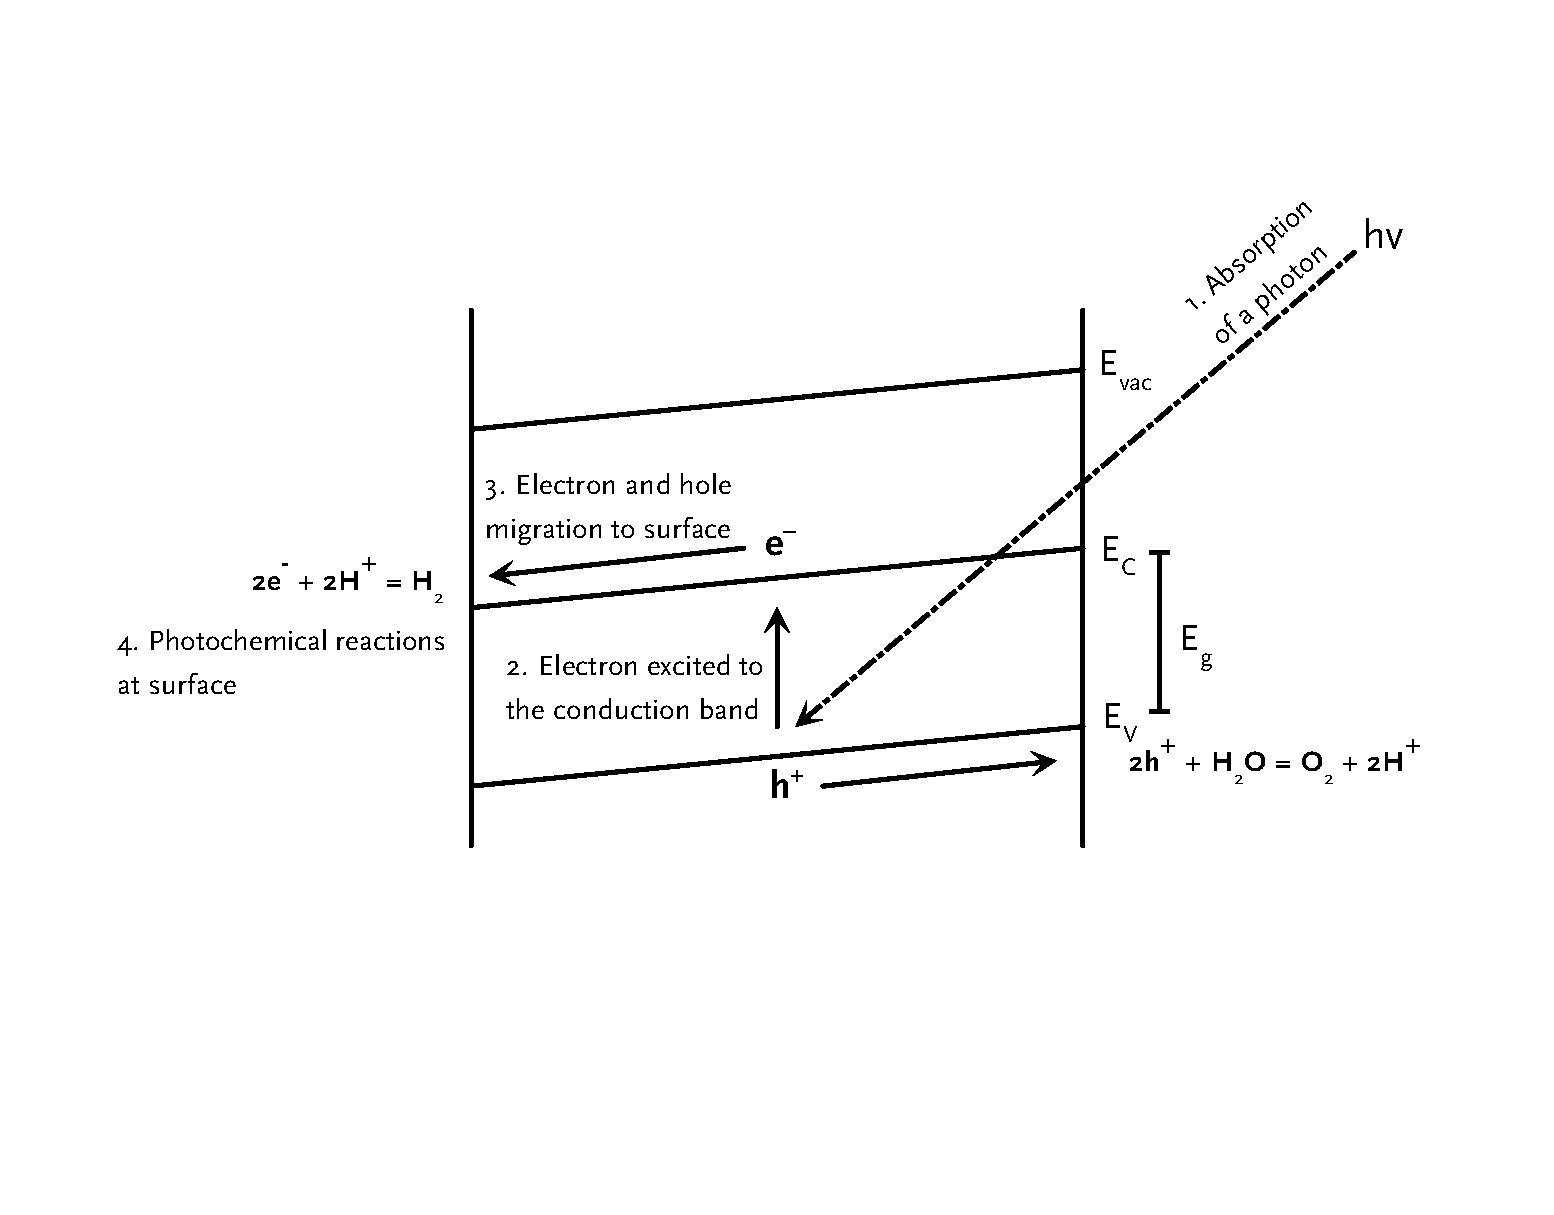
\includegraphics[width=\textwidth]{photochemsteps.pdf}
	\caption[Simplified schematic of the water photolysis process]{%
		Simplified schematic of the water photolysis process. A photon 
		with an energy larger than the band gap is absorbed, exciting 
		an electron from the conduction band to the valence band. The 
		electron and hole are driven to the opposite surfaces by an electric field, 
		represented here by sloped bands. At the surface, the charge 
		carriers take part in photochemical reactions.}
	\label{fig:photochemsteps}
\end{figure}

For water splitting (water photolysis),\cite{memming2001semiconductor} the electrons and holes are used to drive the following reactions:
\begin{gather}
	\ce{2H+ + 2e^{-} -> H2_{(g)}} \hspace{1.5em} \text{(Reduction)}\\
	\ce{H2O + 2h+ -> 1/2O2_{(g)} + 2H+} \hspace{1.5em} \text{(Oxidation).}
\end{gather}
Only electrons and holes with appropriate electrochemical potentials can promote these reactions. The conduction band edge of the semiconductor must lie above the potential of the reduction reaction and the valence band edge must be below the potential for oxidation. An effective photocatalyst has a band gap that is both large enough to promote both reactions and is properly located in relation to the potential of each reaction. For water splitting, the hydrogen and oxygen half reactions are located at 0~V and 1.23~V respectively,\cite{noauthororeditor2007handbook} on the hydrogen scale. This requirement on the band gap and energy levels of potential photolysis catalysts is non-trivial. \figureref{morrisonarray} shows an array of the valence and conduction band energies of potential materials for water photolysis.\cite{Morrison:1980va} Only materials with electron and valence band energies in the white area of the array satisfy both requirements on the position of the energy levels of the semiconductor. Significant research efforts\cite{Osterloh:2008fp} are invested in the discovery and synthesis of new materials that satisfy the necessary energy requirements for water photolysis. 

\begin{figure}
	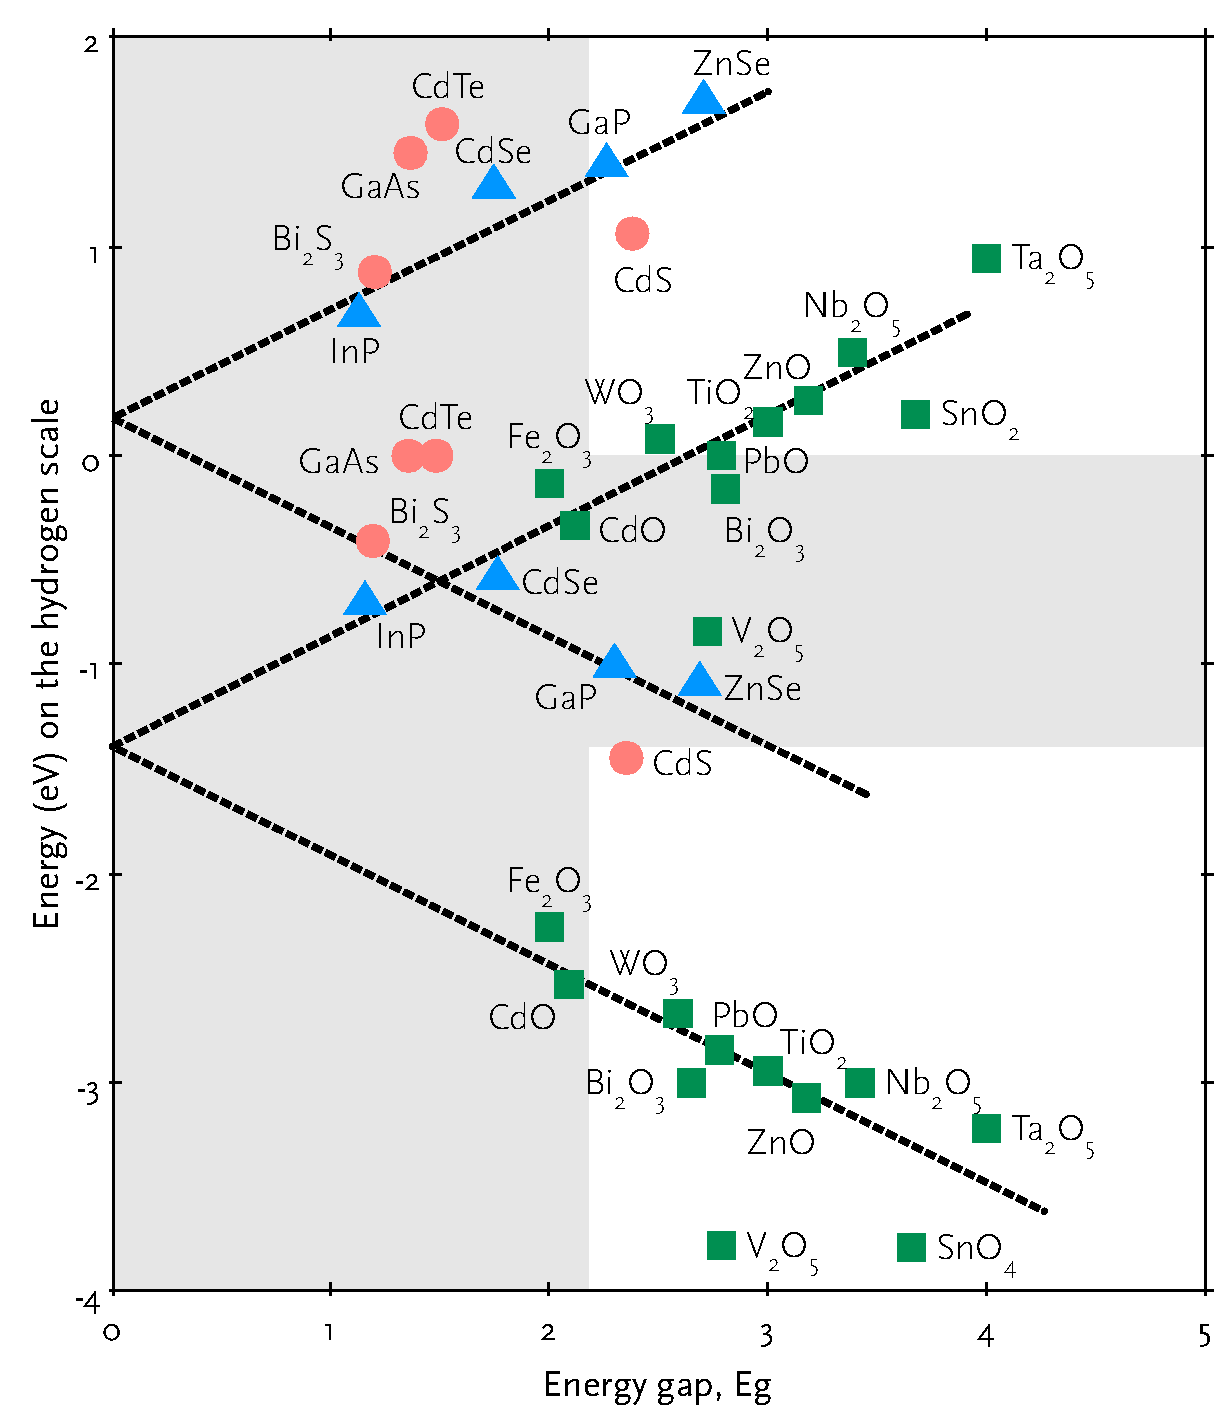
\includegraphics[width=0.95\textwidth]{morrisonarray.pdf}
	\caption[Array of band positions for semiconductors]{%
		Array of band positions for traditional and oxide semiconductors. 
		The area shaded in blue less than \texttildelow2.1~eV represents 
		materials unsuitable for water splitting, as the band gap is not 
		large enough to drive water splitting when overpotentials are 
		considered. The shaded blue area between -1.23~eV and 0 eV on the 
		hydrogen scale represents the position on the energy scale that 
		must be straddled by the band positions. The valence band must be 
		below -1.23 eV and the conduction band must lie above 0~eV.\cite{Morrison:1980va}}
	\label{fig:morrisonarray}
\end{figure}


\subsection{Photolysis and the Solar Spectrum}
\label{subsec:background.solarspectrum}


Before water photolysis can serve as a viable method of hydrogen production, systems must be made less expensive and more efficient. Major limitations on the efficiency of water photolysis are the separation of photogenerated charge carriers in the material and the utilization of a wider portion of the solar spectrum. After a photon is absorbed in a semiconductor and an electron is excited to the valence band, the electron or hole must reach the surface before recombining. Recombination is the process by which a photogenerated charge carrier combines with an oppositely charged carrier. Recombined electron-hole pairs represent lost efficiency, as the recombined electron no longer contains the necessary energy to drive photochemical reactions. 



\begin{figure}
	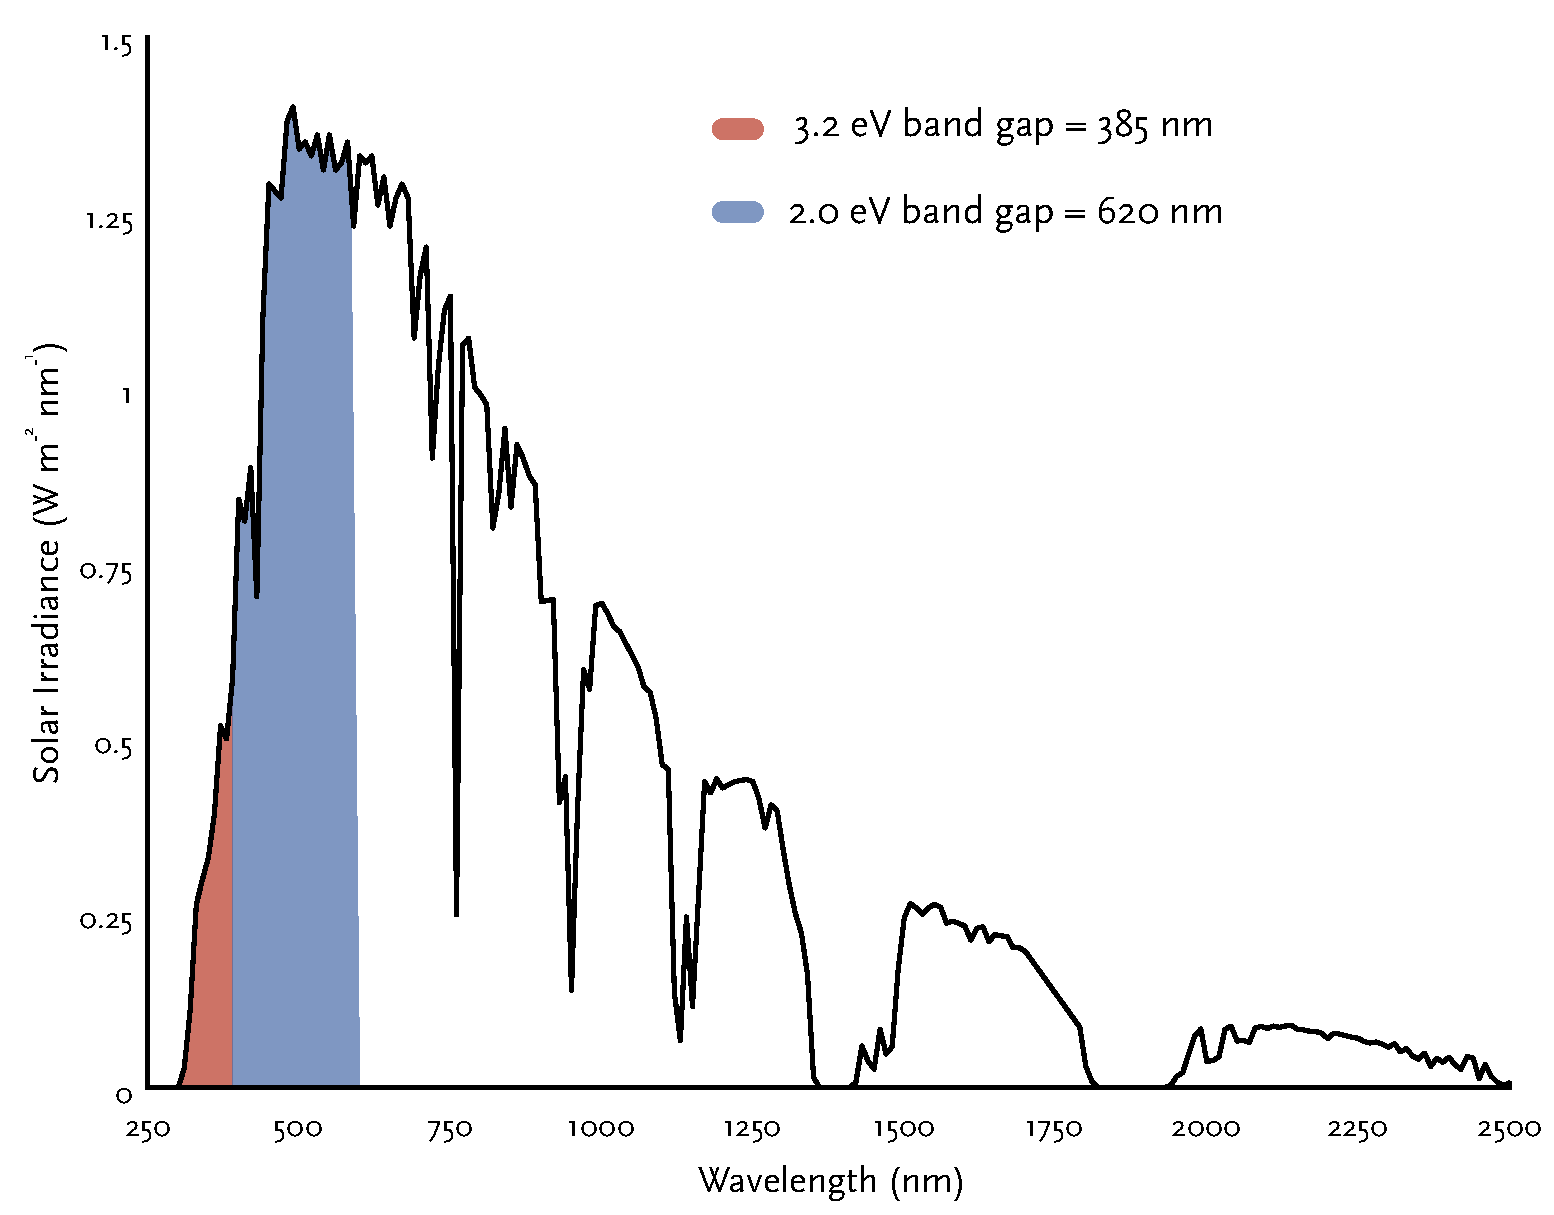
\includegraphics[width=\textwidth]{solarspectrum.pdf}
	\caption[Solar irradiance at the earth 's surface]{%
		Solar irradiance at the earth 's surface as a function of 
		wavelength. The shaded regions represent the portion of the 
		solar spectrum that can be utilized by a semiconductor with a 
		3.2~eV band gap (red) and a 2.0 eV band gap (blue).\cite{Anonymous:jk}}
	\label{fig:solarspectrum}
\end{figure}

The solar spectrum is shown in \figureref{solarspectrum}. The majority of the light reaching the earth's surface lies in the visible range of the electromagnetic spectrum, corresponding to photon energies of 1.6~eV to 3~eV. Titanium dioxide, \ce{TiO2}, one of the most studied photocatalysts, has a band gap of 3.2~eV. This value is well in to the ultraviolet portion of the solar spectrum. Only 2\% of the light reaching the earth's surface is of sufficient energy to excite an electron in \ce{TiO2}. This means that for \ce{TiO2}, 98\% of solar radiation is unavailable for use in water splitting. Moving to materials with a smaller band gap that can utilize light in the visual portion of the spectrum greatly increases the percent utilization of the solar spectrum. A shift to a material with a band gap of 2.0~eV, corresponding to orange light, represents an increased maximum absorption efficiency of using 34\% of the solar spectrum. It should be noted that the absorption efficiency is always greater than the overall efficiency. Each absorbed photon is used to perform 1.23~eV of work, regardless of the energy of the photon. Any excess energy of the photon over the minimum for water splitting represents lost efficiency of the overall system. This goal of shifting to materials with smaller band gaps adds additional complexity to the selection of photolysis catalysts when viewed in connection with \figureref{morrisonarray}. Smaller band gaps are desirable to make use of a wider portion of the solar spectrum, but the band edges must be located correctly in relation to the levels for the reactions of water splitting.

\subsection{Photolysis Systems}
\label{subsec:background.systems}

Currently, research has concentrated on two systems for photolytic hydrogen evolution. The photoelectrochemical cell has shown promising efficiencies,\cite{Fujishima:1972hc,User:2001tg} however it is too expensive for large scale hydrogen production. Particulate photocatalysts have the potential to be much less expensive than photoelectrochemical cells, however their efficiencies are much lower. \cite{Kaneko:2002vh} Because the electrodes in the particle catalysts are not physically separated as in the photoelectrochemical cell, charge carrier recombination limits the efficiency of the catalyst. Much of the work on particulate photocatalysts centers on creating physical separation of the anode (oxidation sites) and cathode (reduction sites).\cite{Kitano:2008io,Kudo:2008fk} Schematics of the photoelectrochemical cell and particulate photocatalyst are depicted in \figureref{pecparticle}.

\begin{figure}
	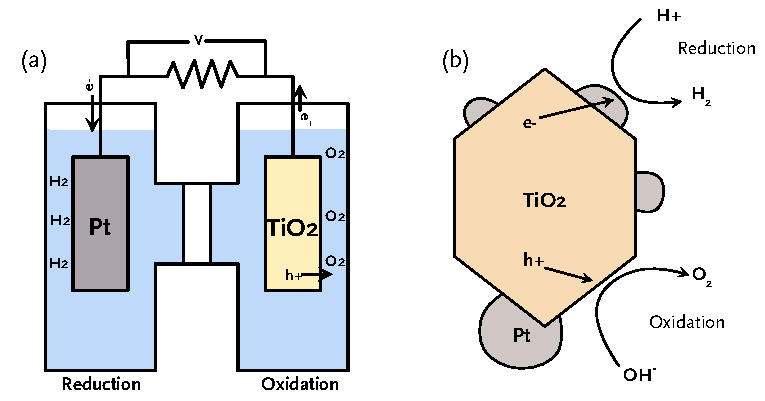
\includegraphics[width=\textwidth]{pecparticle.pdf}
	\caption[Photoelectrochemical and particulate cells]{%
		(a) Photoelectrochemical cell. When light shines on the TiO2 
		electrode, an electron-hole pair is generated. The electron 
		travels through an external `circuit to the platinum electrode, 
		where it generates hydrogen. The hole generates oxygen at the 
		surface of the \ce{TiO2} electrode. (b) A particulate cell. 
		In this case, oxidation and reduction occur on the same particle.}
	\label{fig:pecparticle}
\end{figure}

In the photoelectrochemical cell depicted in \figureref{pecparticle}(a), the \ce{TiO2} electrode is illuminated, generating electrons and holes. The holes participate in oxidation at the \ce{TiO2} electrode, generating oxygen. The electrons travel through an external circuit to a platinum electrode separated by a salt bridge. At the platinum electrode, the electrons reduce hydrogen ions to form hydrogen gas. The particulate catalyst in \figureref{pecparticle}(b) represents a short-circuited version of the photoelectrochemical cell. Electrons and holes are generated in the \ce{TiO2} under illumination. Holes oxidize water at the surface of the \ce{TiO2} surface, while electrons travel to hydrogen particles on the surface, where they participate in reduction.


\subsection{Length Scales in Photochemistry}
\label{subsec:background.lengthscales} %% In response to overview feedback point 7b

\begin{figure}
\begin{center}
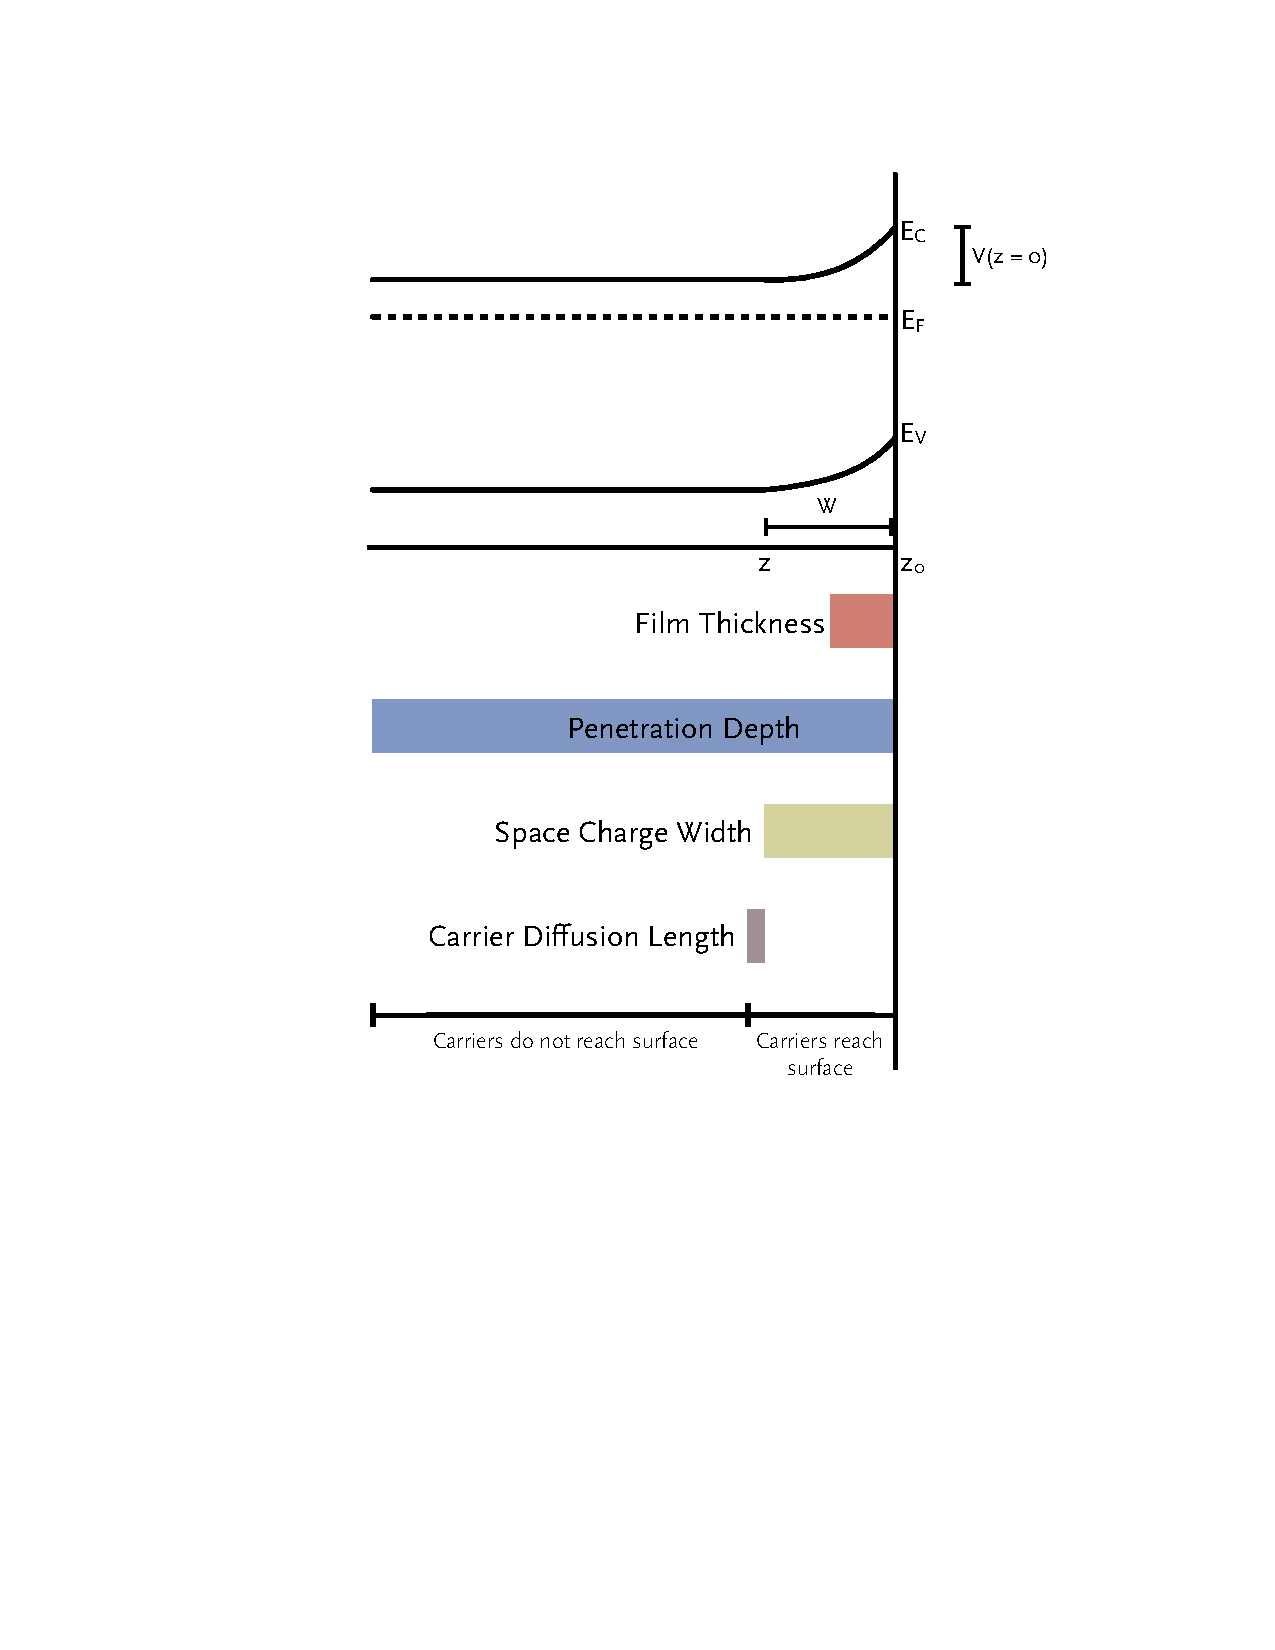
\includegraphics[width=0.6\textwidth]{lengthscales.pdf}
\caption[Band bending at semiconductor surface]{%
	Schematic energy level diagram showing band bending at a semiconductor 
	surface, along with a depiction of typical length scales relevant to 
	semiconductor photochemistry.}
\label{fig:lengthscales}
\end{center}
\end{figure}
%\sidefigure[Band bending at semiconductor surface]{%
%	Schematic energy level diagram showing band bending at a semiconductor 
%	surface, along with a depiction of typical length scales relevant to 
%	semiconductor photochemistry.
%	\label{fig:lengthscales}
%	}{%
%	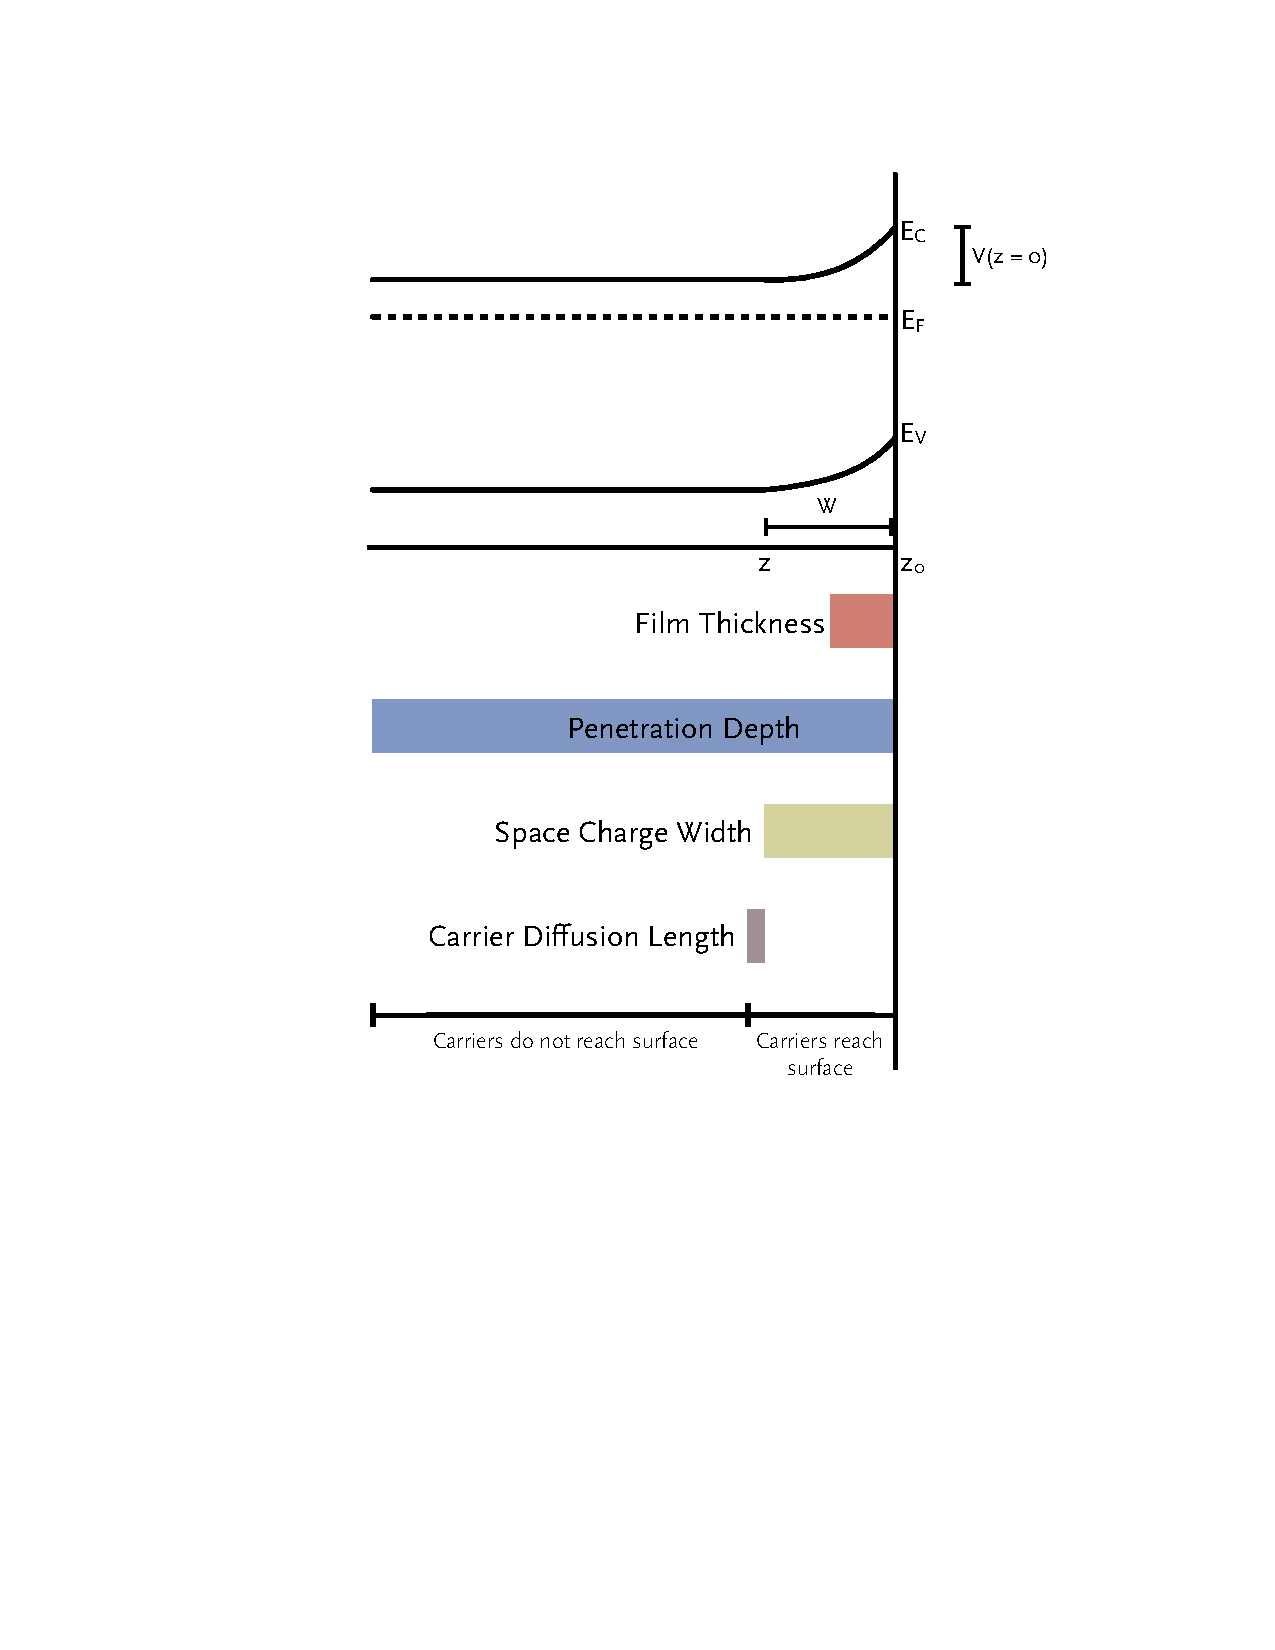
\includegraphics[width=\marginparwidth]{lengthscales.pdf}
%}{0}

A number of competing characteristic length scales play an important role in semiconductor photochemistry. The ideal photolysis catalyst must optimize these characteristic lengths to achieve high efficiencies. The relevant lengths are labelled and compared in \figureref{lengthscales}. Each is discussed in the following section, including its importance to semiconductor photochemistry, relative magnitude, and relation to other relevant parameters.

The penetration depth of light into the semiconductor is the first important length to consider. Not all light is absorbed directly at the surface of the semiconductor. Instead, light penetrates into the semiconductor, its intensity decreasing as it travels further into the crystal and photons are absorbed. The penetration into the crystal is a function of the material's absorption coefficient, which itself is a function of light wavelength. The Beer-Lambert law (Eq. \ref{eq:beerlambert}) describes how the intensity of incident light decays within a material, where $z$ is the depth within the material and $\alpha$ is the absorption coefficient. The penetration depth is defined as the depth within the material where the ratio of intensity to incident intensity is reduced to  $\frac{1}{e}$ (Eq. \ref{eq:definepenetrationdepth}). This point occurs at $\frac{1}{\alpha}$ (Eq. \ref{eq:oneoveralpha}).

\begin{gather}
	\label{eq:beerlambert}
	I(z)=I_{0}e^{-\alpha z},\\
	\label{eq:definepenetrationdepth}
	\delta_{p} \equiv \frac{I(z)}{I_{0}}=\frac{1}{e},\\
	\label{eq:oneoveralpha}
	\delta_{p} = \frac{1}{\alpha}.
\end{gather}

For hematite under illumination by a \SI{470}{\nano\meter} blue LED (the material and light source used in the majority of experiments presented in this document), the penetration depth is \texttildelow\SI{450}{\nano\meter}.\cite{Marusak:1980gc} The majority light absorption occurs within this length, and consequently the majority of electron-hole pairs are generated within this length.

Once an electron-hole pair is generated through the absorption of a photon, it must reach the surface to participate in a chemical reaction. If the electron-hole pair is generated within an electric field,  that field will cause the electron and hole to move in opposite directions, causing one of the carriers to reach the surface. In the heterostructures used for experiments in this document, electric fields arise from built in sources. Details of these sources are presented in \S\ref{sec:background.charged}. In all of the presented cases, the presence of an electric field gives rise to a space charge region. On simple energy level diagrams such as the one in \figureref{lengthscales} and others presented throughout this document, these electric fields are represented by bands bent at an angle relative to the horizontal axis. The width of this space charge region is an important value affecting the photochemical performance of the semiconductor. Only electrons and holes that are generated within or near the space charge region are separated and driven to the semiconductor surface. In the example depicted in \figureref{lengthscales}, a space charge region is shown at the surface of the semiconductor, arising from the presence of surface states. The width of space charge region is governed by the one dimensional Poisson equation in 
\begin{equation}
	\label{eq:poisson}
	\frac{\partial^{2}V}{{\partial}z^{2}}=-\frac{e^{2}N_{D}}{\varepsilon \varepsilon_{0}},
\end{equation}
where $z=0$ is defined as the surface of the material and $N_{D}$ is the dopant density. After integrating twice, the solution takes the form
\begin{equation}
	\label{eq:poissonsolved}
	V(z)=-\frac{e^{2}N_{D}}{2\varepsilon \varepsilon_{0}}(z-z_{0})^{2},
\end{equation}
and if $z$ is defined as 0 at the surface, and $z_{0}$ is the width of the space-charge region (the point where $V=0$), the width $W$ of the space-charge region near the surface is
\begin{equation}
	\label{eq:spacechargewidth}
	-(z-z_{0})=W=\sqrt{\frac{2V_{z=0}\varepsilon}{e^{2}N_{D}}}\text{.}
\end{equation}

A typical value for the width of the space charge region is \SI{100}{\nano\meter}. This means that for \ce{Fe2O3}, a significant portion of light absorption occurs beyond the width of the space charge region at the surface. Electron-hole pairs generated by this light are unlikely to reach the surface of the semiconductor to drive chemical reactions, and thus represent lost energy. Using Equation \ref{eq:definepenetrationdepth}, the total percentage of light absorbed in the first \SI{100}{\nano\meter} for hematite is only \texttildelow20\%. 80\% of the incident light is absorbed beyond the space charge region, and resulting photogenerated charge carriers are unlikely to reach the surface.

As stated in the last paragraph, electrons and holes must be generated within or near the space charge region to be separated and driven to the surface. While charge carriers generated within the space charge region are accelerated by the electric field towards or away from the surface, carriers generated near the space charge region must diffuse to it before they can be driven to the surface.  The carrier diffusion length ($L_{n}$ for electrons and $L_{p}$ for holes) quantifies what specifically is meant by ``near'' the space charge region. The diffusion length is given by

\begin{equation}
	\label{fig:diffusionlength}
	L_{p,n}=\sqrt{D\tau},
\end{equation}
where $D$ is the diffusion coefficient for the charge carrier and $\tau$ is the lifetime of the carrier. Only carriers generated within one diffusion length are likely to reach this region. Any charge carriers generated beyond the space charge width plus one diffusion length will not reach the surface, and represent lost energy. 

In many of the experiments presented in this document, the light absorbing \ce{Fe2O3} material is present in the form of a thin film supported on a wider band gap substrate, \ce{SrTiO3}. In the case of visible light illumination, only the film is capable of absorbing the light. The thickness of the film then plays a major role in determining how much light is absorbed by the heterostructure. If the film is significantly thinner than the penetration depth of the light, a large portion of the incident light passes through the film without being absorbed, reducing the efficiency of the heterostructure. However, if the film is too thick, the band bending effects arising from the substrate-film interface described in \sectionref{sec:background.charged} will be completely screened by charge carriers in the film. The film thickness must selected to ensure that a sufficient amount of light is absorbed (favoring a thicker film) while interface effects are not completely screened (favoring a thinner film).


\subsection{Surface Activity Considerations}
\label{subsec:background.surfaceactivity}


Surface roughness can significantly affect the photochemical properties of a semiconductor surface. Given two otherwise identical semiconductors, one with a rough surface and the other smooth, the sample with the rougher surface has a higher surface area exposed and, therefore, is expected to be more photochemically active. Photogenerated electron and holes must interact with species in solution to participate in chemical reactions. With a higher surface area, more reaction sites are available for the charge carriers and reaction species to interact, the reaction rate increases. This is one of the drivers of research into high surface area nanoparticles and films for photochemical applications.\cite{Kudo:2008fk} For this reason, photochemical activity is often normalized by the active material's surface area. Where relevant, the affect of surface roughness on the interpretation of results is included in the results sections of this document.

%\subsection{Electrochemical Considerations}
%\label{subsec:background.electrochem} Move this material into relevant experimental sections or results sections
%
%
%Significant overlap exists between the fields of electrochemistry and semiconductor photochemistry. In particular, when considering the complete system of the semiconductor, the solution, and their interface, certain electrochemical concepts such as pH, mass transfer, and energy level alignments should not be ignored. These topics are discussed briefly, along with their relevance to the results presented in this document, in the following subsections. \textcolor{red}{Does this section belong here, or should it go by the introduction of marker reaction, or by the first time we get results from the marker reaction? I'm not sure it's important enough to merit its own section in the background, since I end up just discounting these effects.}
%
%
%\subsubsection{pH Effects}
%\label{subsubsec:background.ph}
%
%
%\subsubsection{Mass Transfer}
%\label{subsubsec:background.masstransfer}




\section{Charged Interfaces and Surfaces}
\label{sec:background.charged}

\begin{figure}
\begin{center}
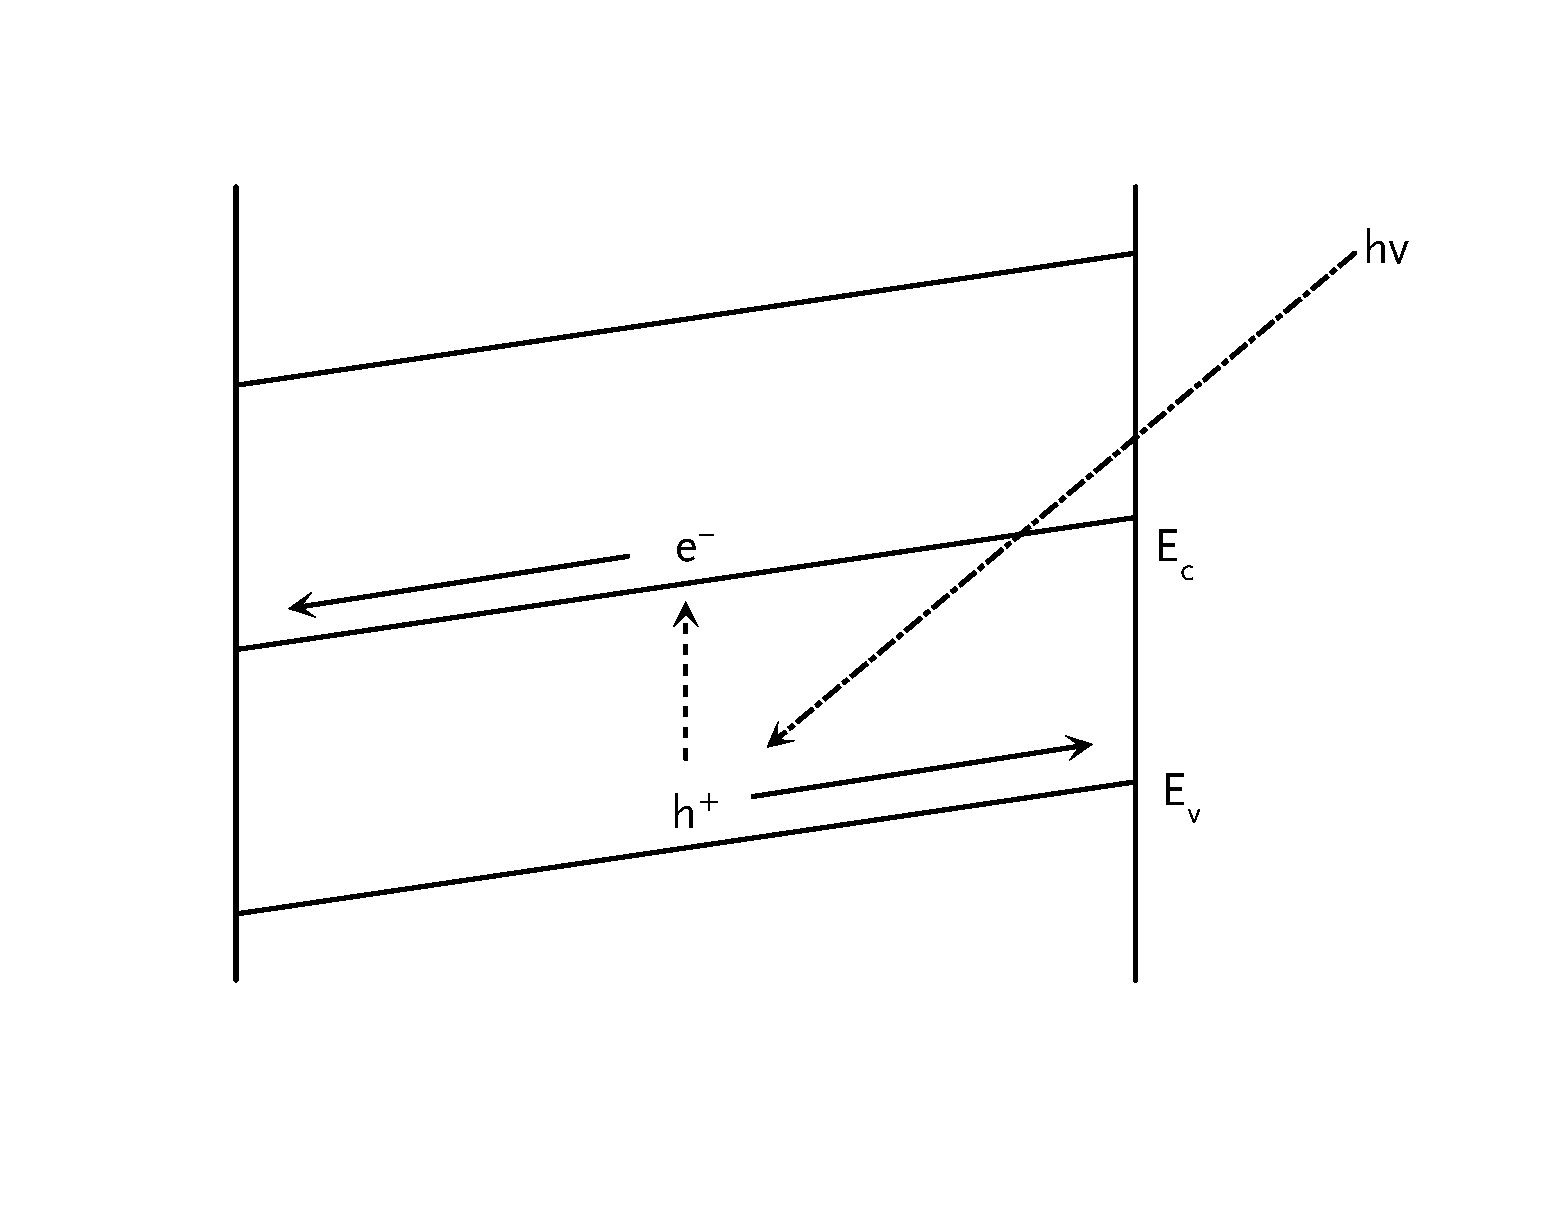
\includegraphics[width=0.8\textwidth]{electronholemovement.pdf}
\caption[Movement of photogenerated charge carriers]{%
	Simplified energy level diagram showing the movement of photogenerated charge carriers in an electric field. The electric field is represented by the sloped bands. Electrons move down on the band to lower energy states, while holes move up.}
\label{fig:electronholemovement}
\end{center}
\end{figure}
%\sidefigure[Movement of photogenerated charge carriers]{%
%	Simplified energy level diagram showing the movement of photogenerated charge carriers in an electric field. The electric field is represented by the sloped bands. Electrons move down on the band to lower energy states, while holes move up.
%	\label{fig:electronholemovement}
%	}{%
%	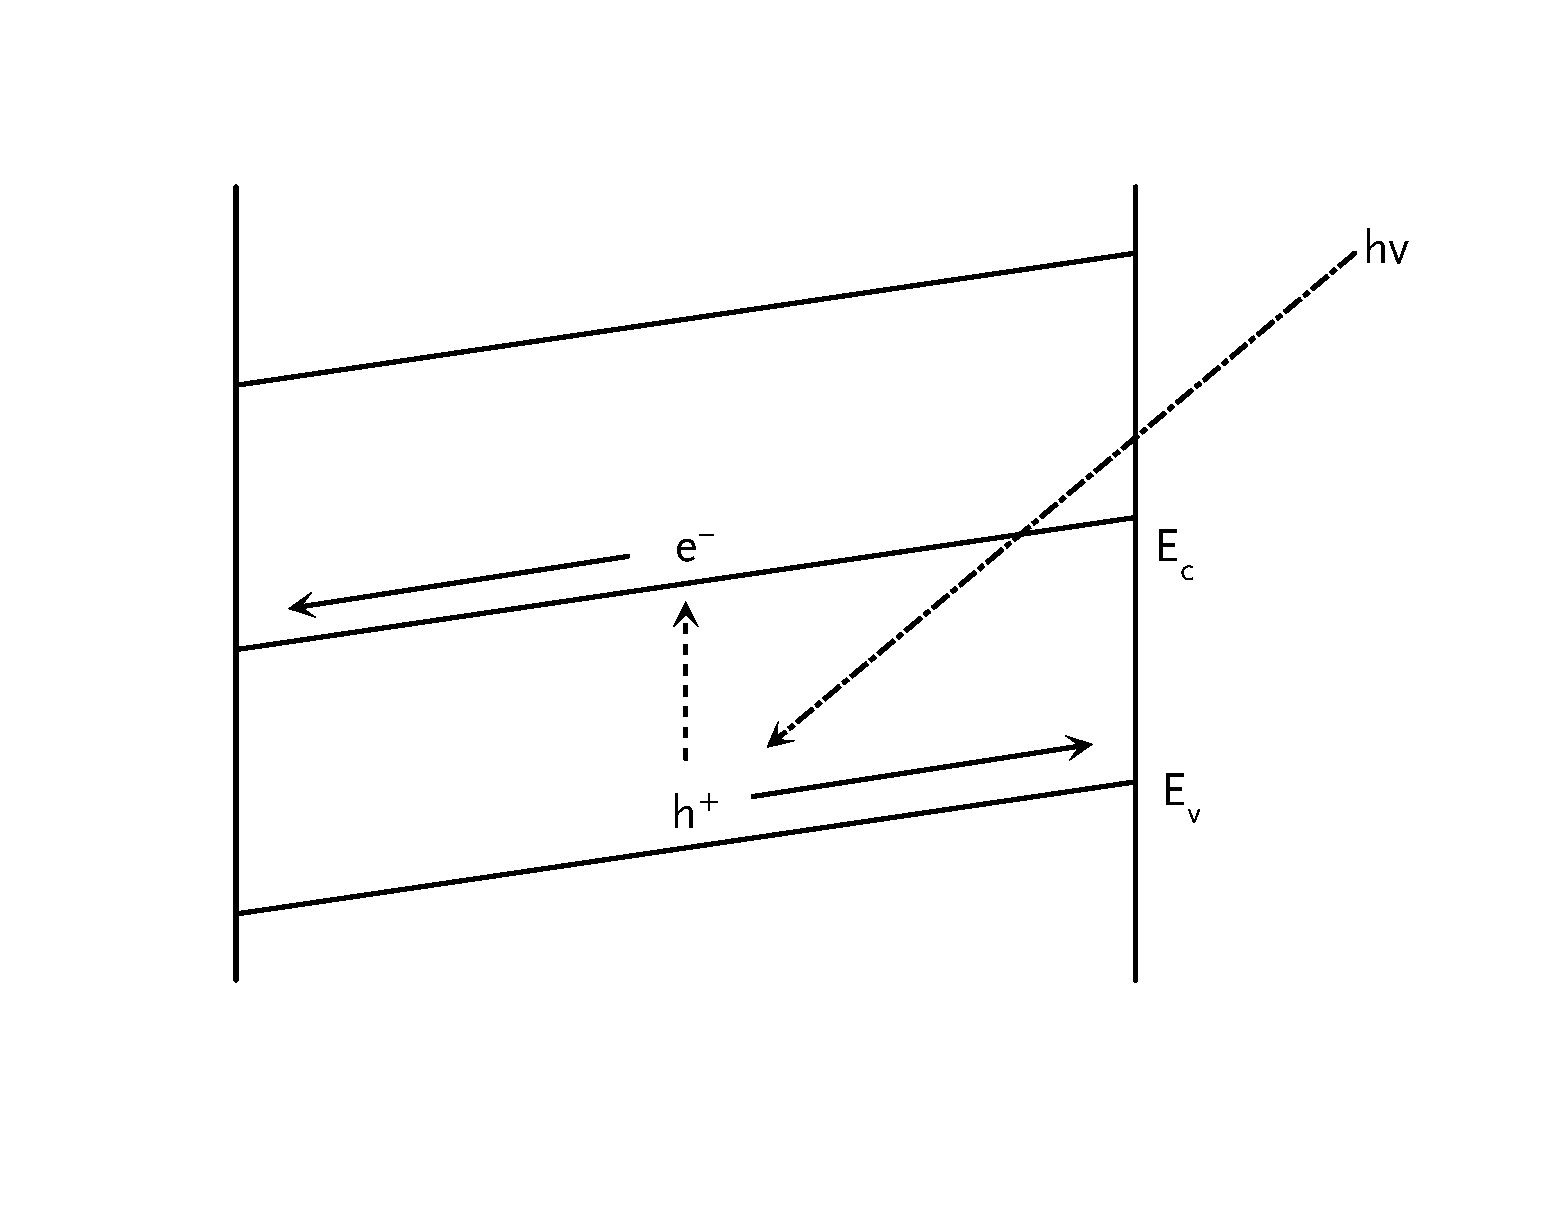
\includegraphics[width=\marginparwidth]{electronholemovement.pdf}
%}{0}


Under the presence of an electric field, electrons and holes are physically separated in a material. The electric field drives electrons and holes in the opposite direction. This is shown schematically in \figureref{electronholemovement}. In simple energy level diagrams such as the one depicted in \figureref{electronholemovement}, electric fields are represented by bands that are angled with respect to the horizontal axis. Electrons are accelerated towards a lower energy state by electric fields, corresponding to traveling ``downhill'' on the band diagram. The reverse is true of holes. Holes are driven ``uphill'' to higher energy states. The presence of electric fields is desirable in the case of photochemistry, as the fields can be engineered to drive electrons or holes to the sample surface, where they can participate in chemical reactions. Electrons and holes that do not reach the surface of the material are eventually lost to recombination, reducing the photochemical efficiency. Heterostructure interfaces are an an established method of generating electric fields within a material. Three possible sources of electric fields in heterostructured interfaces are discussed in this section, including p-n junctions, ferroelectrics, and polar surface terminations. Each of these cases is depicted schematically in \figureref{chargedinterfaces}. 

\begin{figure}

	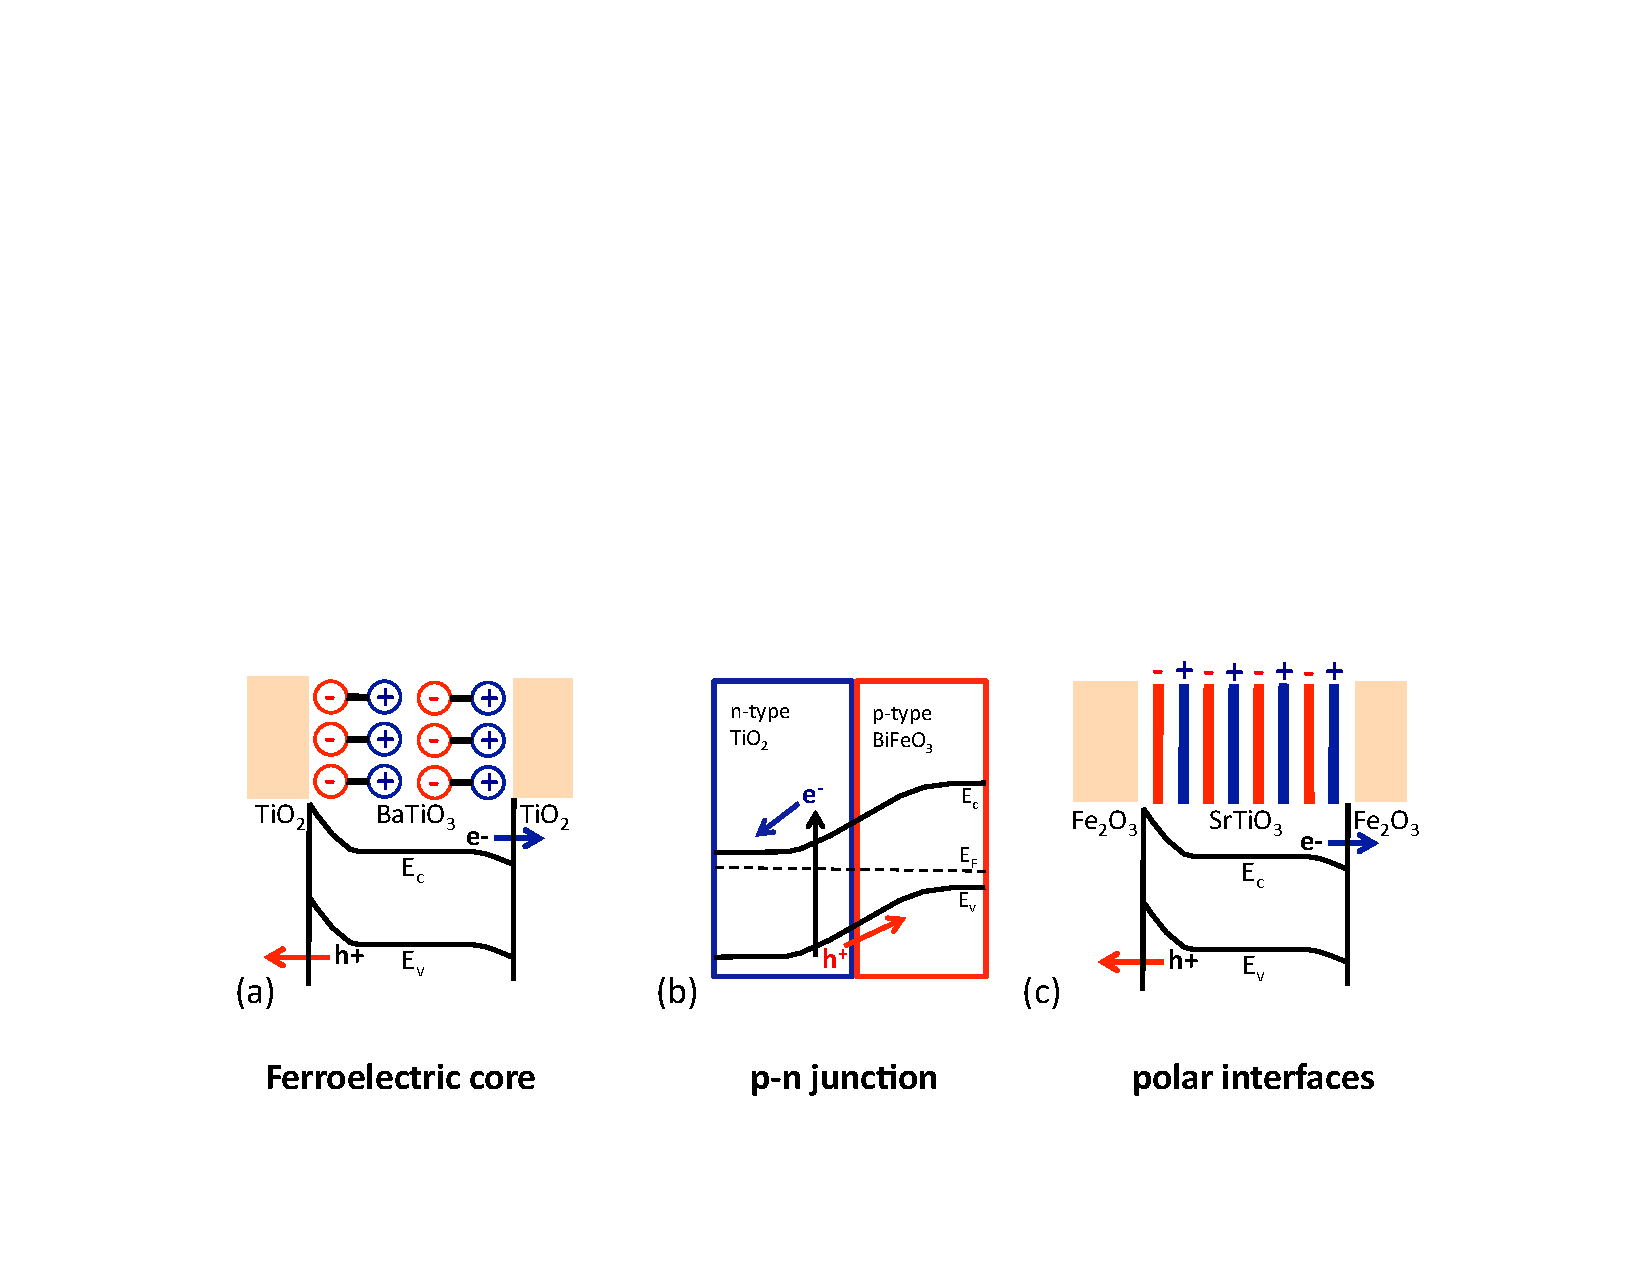
\includegraphics[width=\textwidth]{chargedinterfaces.pdf}
		\caption[Three sources of charged interfaces]{%
			Three sources of charged interfaces. (a) Polarization from a 
			ferroelectric \ce{BaTiO3} core causes electric fields at the 
			surface of a \ce{TiO2} shell. (b) A p-n junction. At the 
			interface, electrons and holes are driven in opposite directions 
			by an electric field as a result of the p-n junction formed by 
			n-type \ce{TiO2} and p-type \ce{BiFeO3}. (c) Uncompensated 
			charge at the interface between a core and film causes electric 
			fields. The charge arises from incompletely compensated polar 
			surface terminations at the interface between \ce{SrTiO3} and 
			\ce{TiO2}.}
	\label{fig:chargedinterfaces}

\end{figure}


\subsection{p-n Junction}
\label{subsec:background.pnjunction}


The presence of a p-n junction has long been known to separate photogenerated charge carriers. A p-n junction arises when a semiconductor with an excess of negative charge carriers (n-type) is placed in contact with a semiconductor with an excess of positive charge carriers (p-type). Excess charge carriers arise in semiconductors as a result of intentional doping with impurity atoms, or as a result of the processing conditions of the material. An intrinsic semiconductor, as in the case of pure silicon, has an equal concentration of electrons and holes. By including a small amount of an impurity element with more or fewer electrons in its valance shell than silicon, the semiconductor can be made p-type or n-type. For example, the inclusion of arsenic in a silicon semiconductor will make the silicon n-type. Arsenic has a five valence electrons, one more than silicon's four, contributing one excess electron for every arsenic atom. If boron, with three valence electrons, is added to pure silicon, the net result is one fewer electron in the material for each boron atom. This ``missing'' electron is termed a hole, and has a positive charge equal in magnitude to the charge on an electron. When studying semiconductors, it is useful to describe the hole as a particle, even through it actually represents the absence of an electron. 

In oxide semiconductors, including all the materials discussed in this document, the bulk oxide often shows p-type or n-type conductivity even in the absence of intentional doping. This arises as a result of the processing conditions. The presence of oxygen vacancies gives rise to n-type oxides, while the presence of metal vacancies gives rise to p-type oxides. The defect reactions corresponding to the formation of oxygen or metal vacancies are:
\begin{align}
	\ce{MO}&\ce{-> M_M + V_O^{\bullet\bullet} + 2e- + 1/2O2_{(g)} \hspace{1em} \text{(Oxygen~vacancy)}} \\
	\ce{MO}&\ce{-> O_O + V_M^{$\prime\prime$} + 2h+ + M_{(g/l/s)} \hspace{1em} \text{(Metal~vacancy)}}
\end{align}
Oxygen vacancies arise through equilibrium with the atmosphere during material fabrication. Increased oxygen partial pressure in during sintering leads to a decrease in oxygen vacancy concentration, and as a result, excess electron concentration. Volatile metal metal elements often lead to metal vacancies during high temperature sintering. For example, bismuth is easily lost to the atmosphere during the sintering of \ce{BiFeO3}, the photochemical properties of which are discussed in this document. The loss of bismuth during sintering leads to its p-type conductivity. Additionally, aliovalent substitution leads to increased charge carriers. For example, the presence of an ion in the $4^{+}$ oxidation state on a $3^{+}$ site leads to on extra free electron.

When n-type and p-type materials are joined, electrons near the junction in the n-type material diffuse into the p-type material, leading to charged regions. The missing electrons in the n-type region leave a region of net positive charge. The excess electrons that have diffused into the p-type material lead to a region of  negative charge. These charged regions, collectively termed the space charge regions, give rise to an electric field. The field drives electrons and holes in opposite directions. If electrons-hole pairs are generated in the region of the electric field, the electrons are driven toward the n-type material, while holes are driven to the p-type material. The formation of the p-n junction and the resulting effect on photogenerated electron hole pairs are shown in \figureref{pnjunction}.

\begin{figure}
	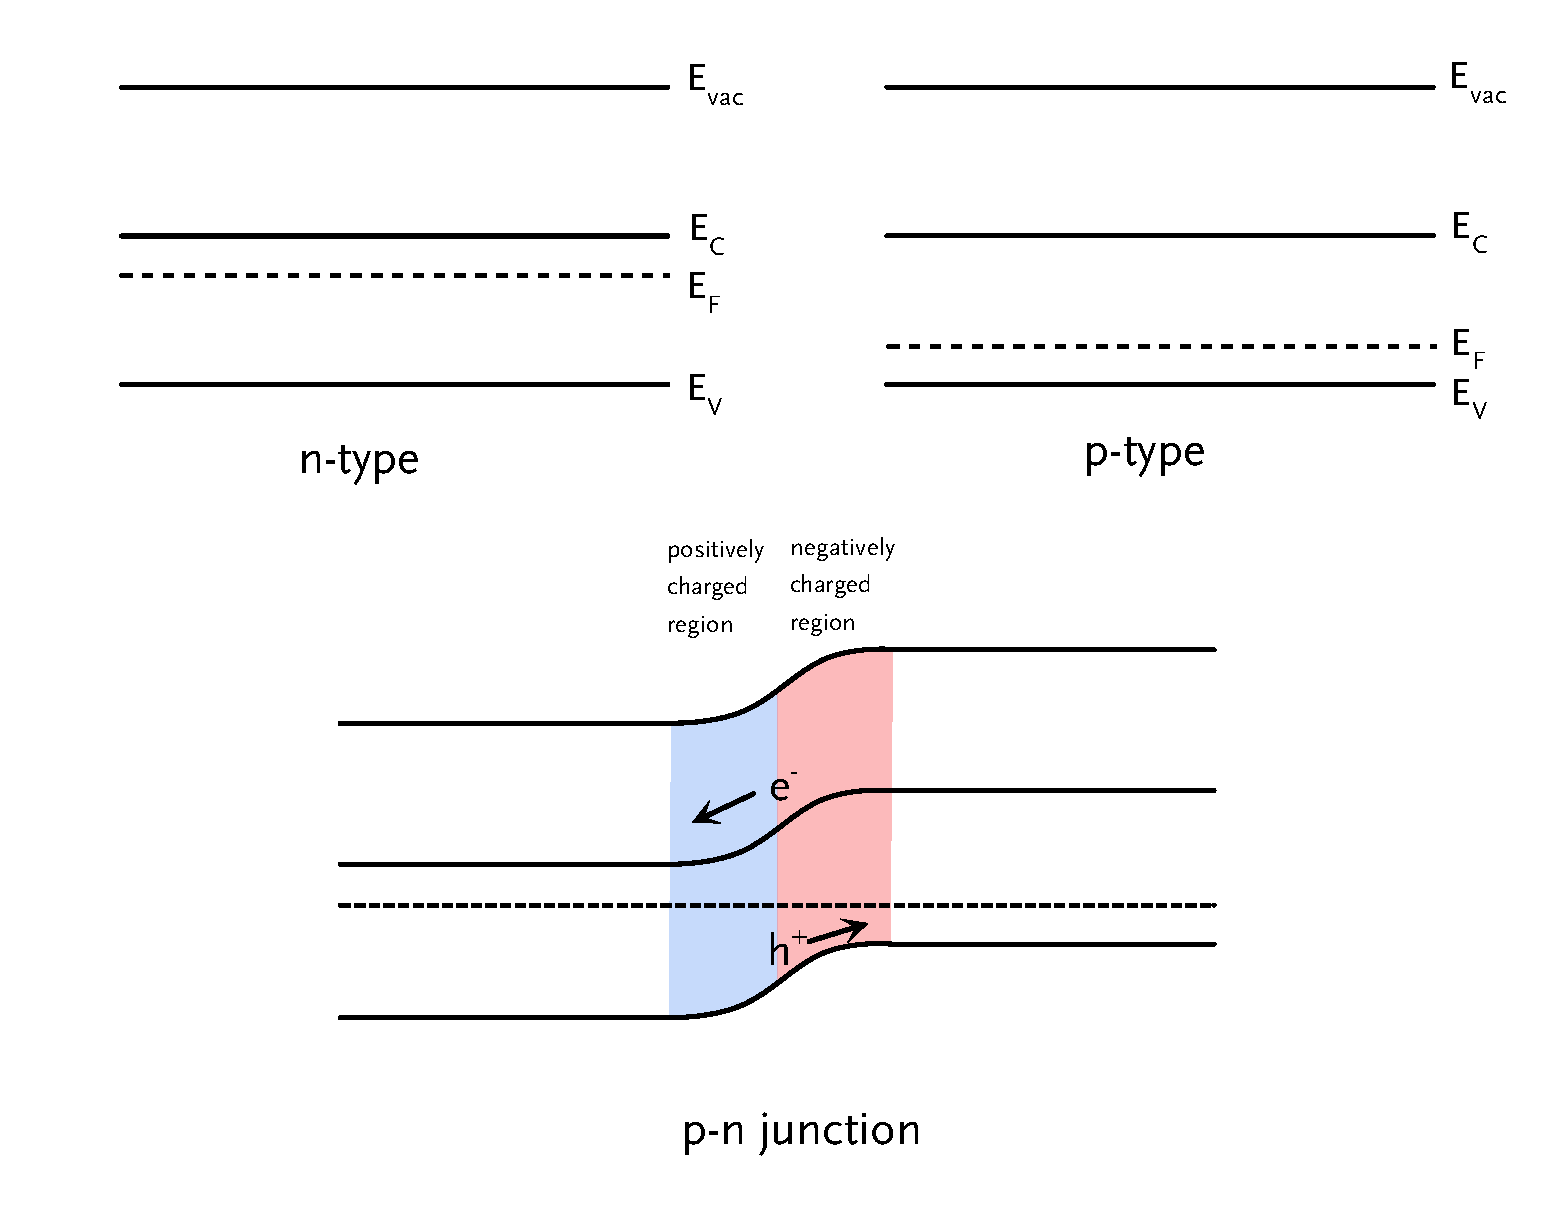
\includegraphics[width=\textwidth]{pnjunction.pdf}
		\caption[The formation of a p-n junction]{%
			The formation of a p-n junction. When an n-type and p-type 
			semiconductor are brought in contact, their Fermi levels 
			align as electrons move from the n-type material into the 
			p-type material. An electric field is created at the 
			interface that drives photogenerated charge carriers in 
			opposite directions.}
	\label{fig:pnjunction}
\end{figure}

The p-n junction is the foundation for conventional solar photovoltaic technology. The photogenerated charges separated by the p-n junction are collected at either end of the device, resulting in a direct current. The same phenomenon also has potential use in photochemical devices, increasing the likelihood of photogenerated charge carriers reaching the surface of the semiconductor, where they can participate the chemical reactions. 


\subsection{Ferroelectric Polarization}
\label{subsec:background.ferroelectric}


Ferroelectrics are a subclass of a group of materials called piezoelectrics. Piezoelectrics are materials that exhibit an electrical polarity under an applied mechanical stress. The reverse is also true; piezoelectric materials deform under an applied electric field. \cite{Lines:1977ug} All piezoelectrics belong to one of the non-centric crystal classes. When a stress is applied to a centrosymmetric crystal, any movement of charge is symmetric, resulting in no net polarization. Charge movement is not symmetric when stress is applied to most non-centrosymmetric crystals, resulting in a net polarization across the crystal. \cite{Lines:1977ug}

Ferroelectric materials exhibit spontaneous polarization below a specific temperature, called the Curie temperature \ce{T_c}, in the absence of an electric field. \cite{Lines:1977ug} Multiple orientational configurations of the polarization vector exist, and an applied electric field can switch the orientation of the polarization vector from one state to another.\cite{Lines:1977ug,Anonymous:7uC1r_sG} As the temperature of a ferroelectric material is lowered below the Curie temperature, different regions of the crystal polarize in each of the different directions. These regions of uniform polarization are called domains.\cite{Lines:1977ug,Anonymous:7uC1r_sG,ForsberghJr:1949vl}

At the surface of the crystal, the termination of the ferroelectric polarization gives rise to a depolarization field. Charge carriers within the crystal can move to the surface to counteract this field. If the field is perfectly compensated by charge carriers, then the energy associated with the depolarization field is zero. However, if the conductivity of the material is low, this compensation could take a very long time, resulting in high energies associated with the depolarization field. However, the formation of domains acts to minimize the energy associated with depolarization fields. The boundaries between domains, across which the polarization vector changes, are called domain walls. Domain walls are usually classified by the angle between the polarization vector on each side of the boundary. As the domain walls stray from the ideal crystal lattice arrangement, a nonzero energy is associated with their formation. The overall domain configuration of the crystal is determined in general by the balancing of the energy gained by reducing the depolarization fields and the energy cost of forming domain walls.

It has been shown that, for ferroelectric materials such as \ce{BaTiO3}, the domain structure effectively promotes photochemical oxidation and reduction on spatially distinct areas of the surface. \cite{Giocondi:2001gz,Burbure:2010go,Giocondi:2003ub,Giocondi:2001bi} Domains with a positive polarization at the surface promote photochemical reduction, while domains with a negative surface polarization promote oxidation. The ferroelectric polarization acts to bend the bands at the surface. The positive polarization bends the bands downward, driving electrons to the surface. The negative polarization bends the bands upward, driving holes to the surface. This effect is shown schematically in \figureref{ferroelectric}. Similar effects have also been observed in ferroelectric \ce{Pb(Zr_{x}T_{1-x})O3} (\abbr{PZT}) and \ce{LiNbO3}.\cite{Hanson:2006bq,Kalinin:2002iw,Tiwari:2009jv}

\begin{figure}
	\centerline{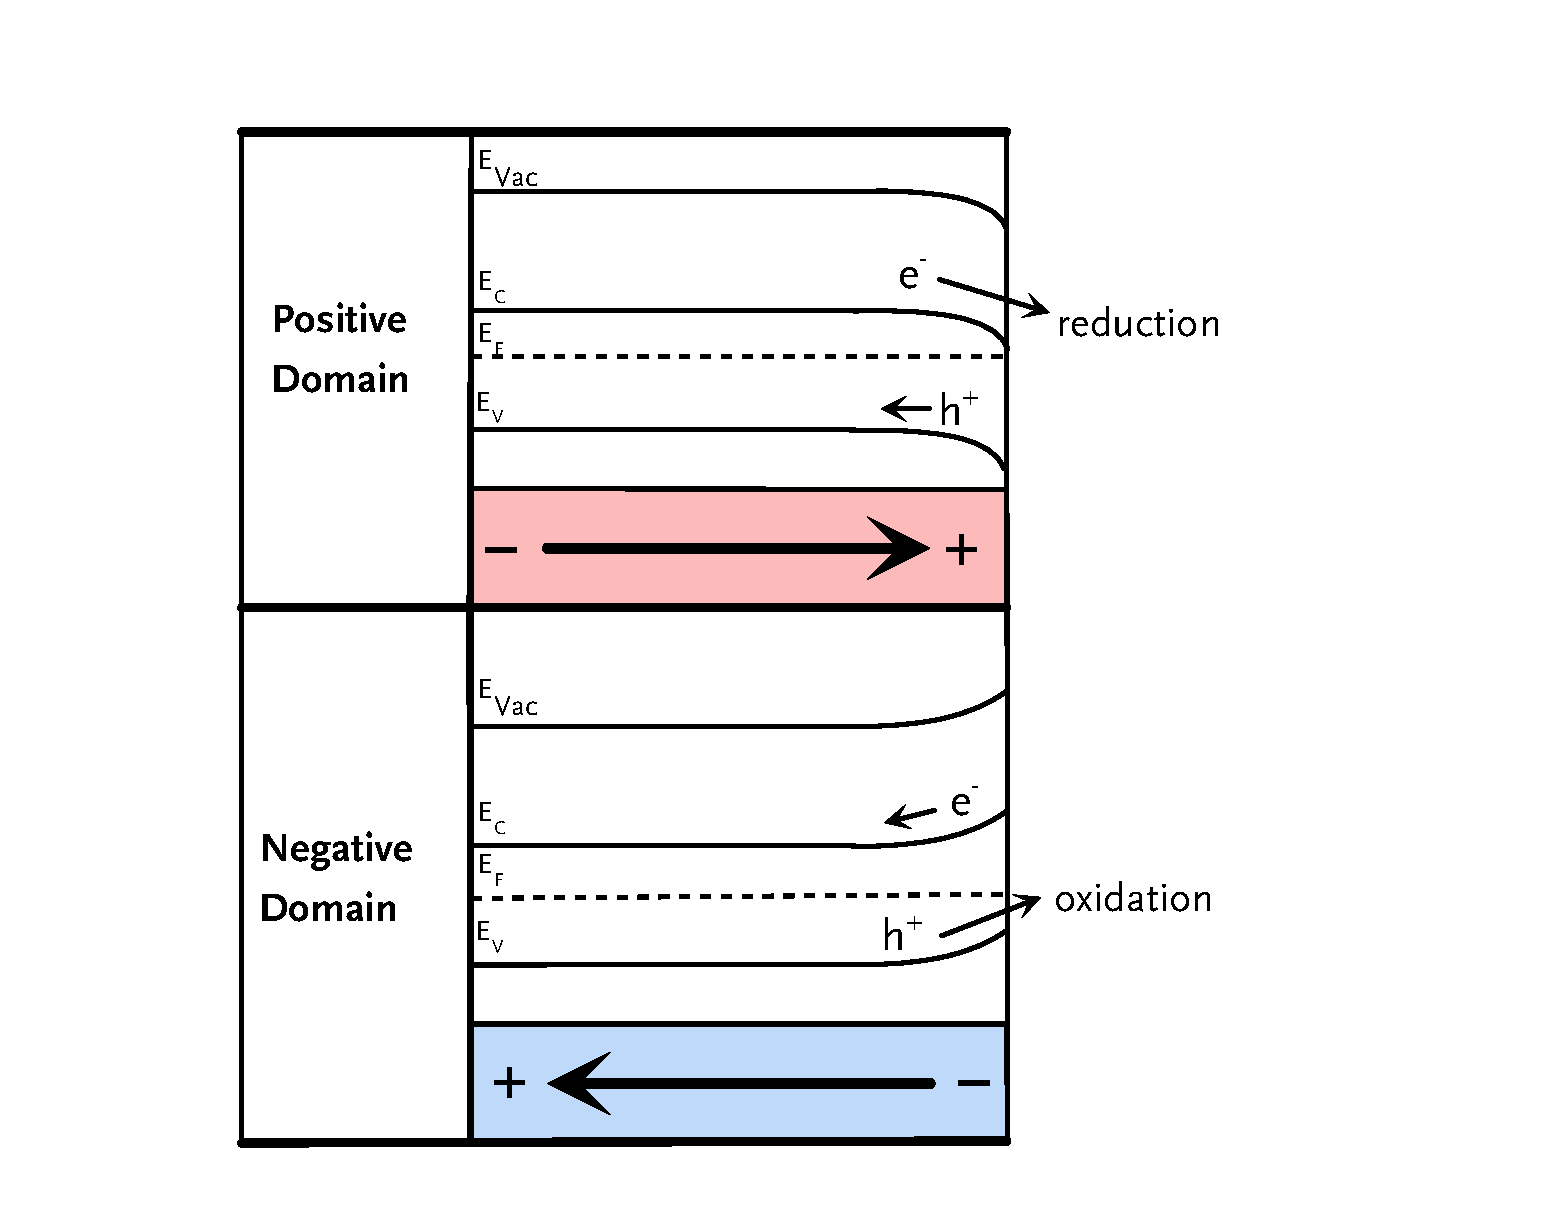
\includegraphics[width=0.8\textwidth]{ferroelectric.pdf}}
	\caption[Band bending at the surface of ferroelectric domains]{%
		Band bending at the surface of ferroelectric domains. A positive 
		domain has the bands bent downward at the surface, favoring 
		reduction. A negative domain has the band bend upwards, favoring 
		oxidation.}
	\label{fig:ferroelectric}
\end{figure}

By driving charge carriers in opposite directions, the ferroelectric fields reduce the recombination rates of electron-hole pairs generated in the space charge region near the surface of the ferroelectric. Additionally, because oxidation and reduction are occurring on distinct areas of the sample surface, the ferroelectric fields are hypothesized to reduce the rate of back reaction of intermediate products in the water splitting process. Burbure\cite{Burbure:2010go,Burbure:2006cq,Burbure:2010ti} demonstrated that the spatial separation of oxidation and reduction from ferroelectric domains persists, even when a thin film of \ce{TiO2} was deposited on \ce{BaTiO3}. This phenomenon suggest the possibility of increased photochemical efficiency through the inclusion of ferroelectric interfaces.


\subsection{Polar Terminations}
\label{subsec:background.polarterms}


\begin{figure}
\begin{center}
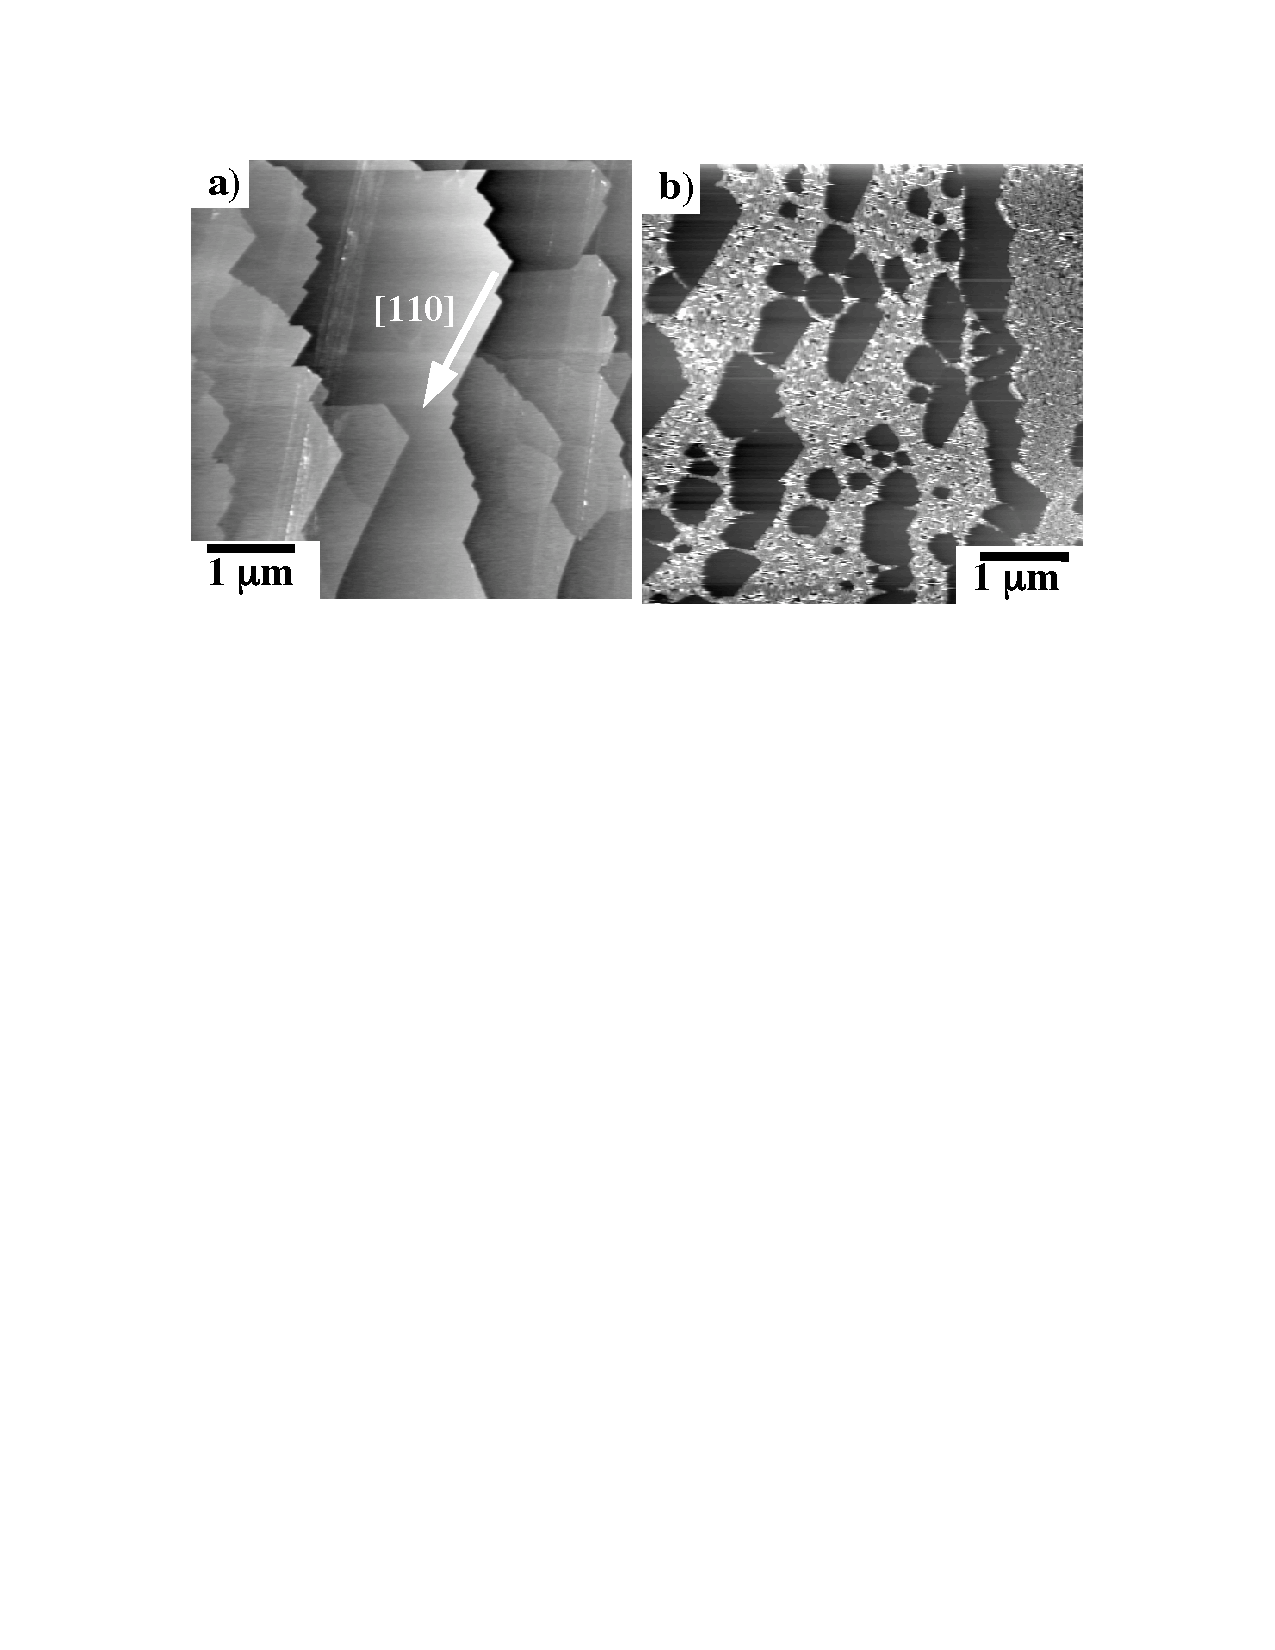
\includegraphics[width=0.8\textwidth]{giocondi.pdf}
\caption[Surface of an annealed \ce{SrTiO3} (111) single crystal]{%
	The surface of an annealed \ce{SrTiO3} (111) single crystal before 
	(a) and after (b) reaction with \ce{AgNO3}. The silver is preferentially 
	deposited on certain faces, corresponding to surfaces of different 
	polar terminations.\cite{Giocondi:2003wc}}
\label{fig:giocondi}
\end{center}
\end{figure}
%\sidefigure[Surface of an annealed \ce{SrTiO3} (111) single crystal]{%
%	The surface of an annealed \ce{SrTiO3} (111) single crystal before 
%	(a) and after (b) reaction with \ce{AgNO3}. The silver is preferentially 
%	deposited on certain faces, corresponding to surfaces of different 
%	polar terminations.\cite{Giocondi:2003wc}
%	\label{fig:giocondi}
%	}{%
%	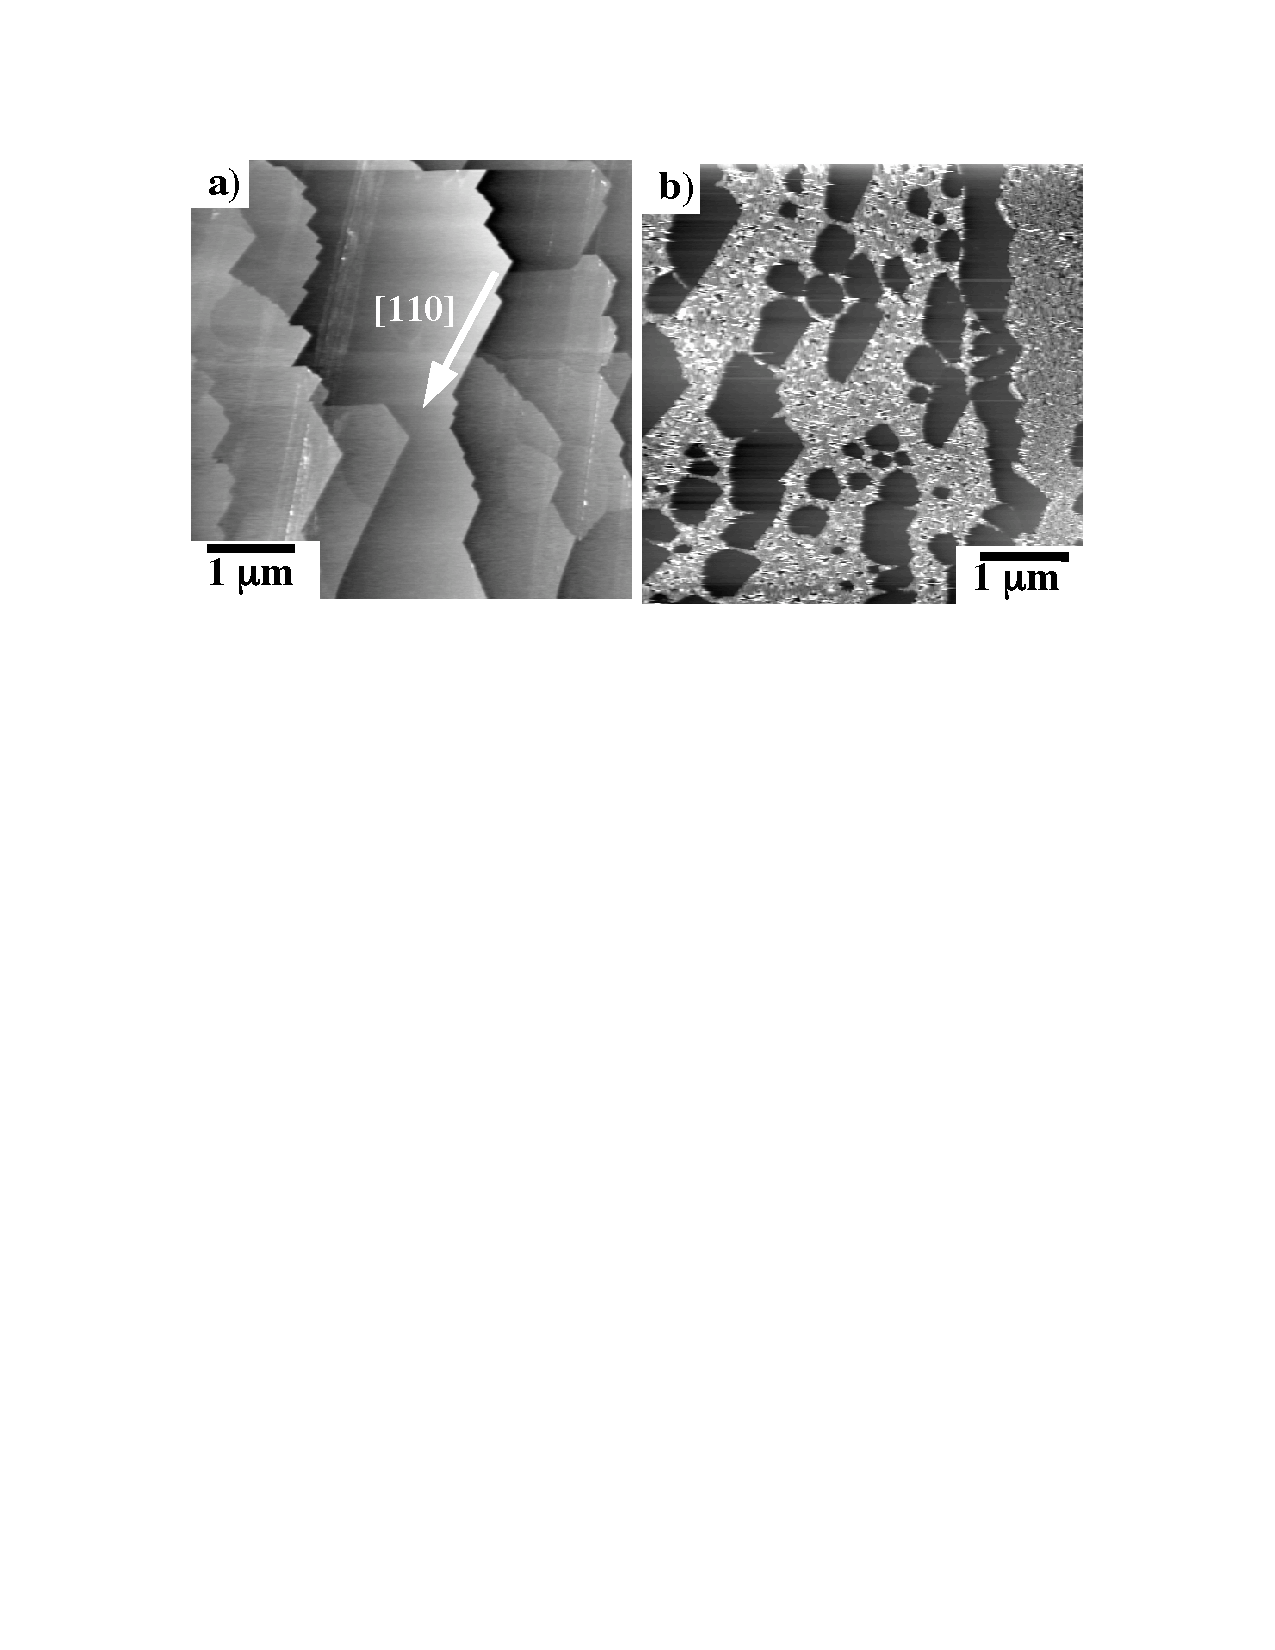
\includegraphics[width=\marginparwidth]{giocondi.pdf}
%}{-2}
Giocondi\cite{Giocondi:2003wc} discovered that polar surface terminations can also result in spatially selective photochemical reactivity on the surface of \ce{SrTiO3}. \figureref{giocondi} shows the surface of a (111) \ce{SrTiO3} single crystal before and after photochemical reaction with aqueous silver nitrate. The bright areas on the surface after reaction correspond to the reduced solid silver reaction product. The silver does not cover the entire surface. Instead, it appears as regions of total coverage and regions of no coverage. The shapes of these regions appear similar to the shapes of the terraces before reaction. Giocondi attributed this spatially selective reaction to the two possible surface terminations of the (111) \ce{SrTiO3} surface. As discussed in more detail in \sectionref{subsubsec:background.sto} on \ce{SrTiO3} crystallography, (111) \ce{SrTiO3} surfaces are terminated by either \ce{SrO3^{4-}} or \ce{Ti^{4+}} layers. After measuring the step heights between the terraces on the clean surface, it was determined that regions of similar reactivity correspond to terraces separated by an even multiple of the spacing between lattice planes. Areas of differing reactivity were separated by an odd multiple. From this information, it was concluded that the areas of high reactivity shared the same termination, and all nonreactive areas shared the other termination.

It was hypothesized that the charge at these surfaces could lead to the presence of a space charge region at the surface, similar to that for ferroelectric polarization. Terraces with a \ce{SrO3^{4-}} termination have a negative surface charge, associated with a upward band bending at the surface. \ce{Ti^{4+}} terminated surfaces have a positive surface charge, leading to negative band bending. This hypothesis is illustrated schematically in \figureref{polarterminations}. Up to this point, the effect of polar surface terminations on the photochemical reactivity of supported films has not been tested. The effect of the polar surface terminations of (111) \ce{SrTiO3} on the reactivity of hematite films is reported in this document.
\begin{figure}
	\centerline{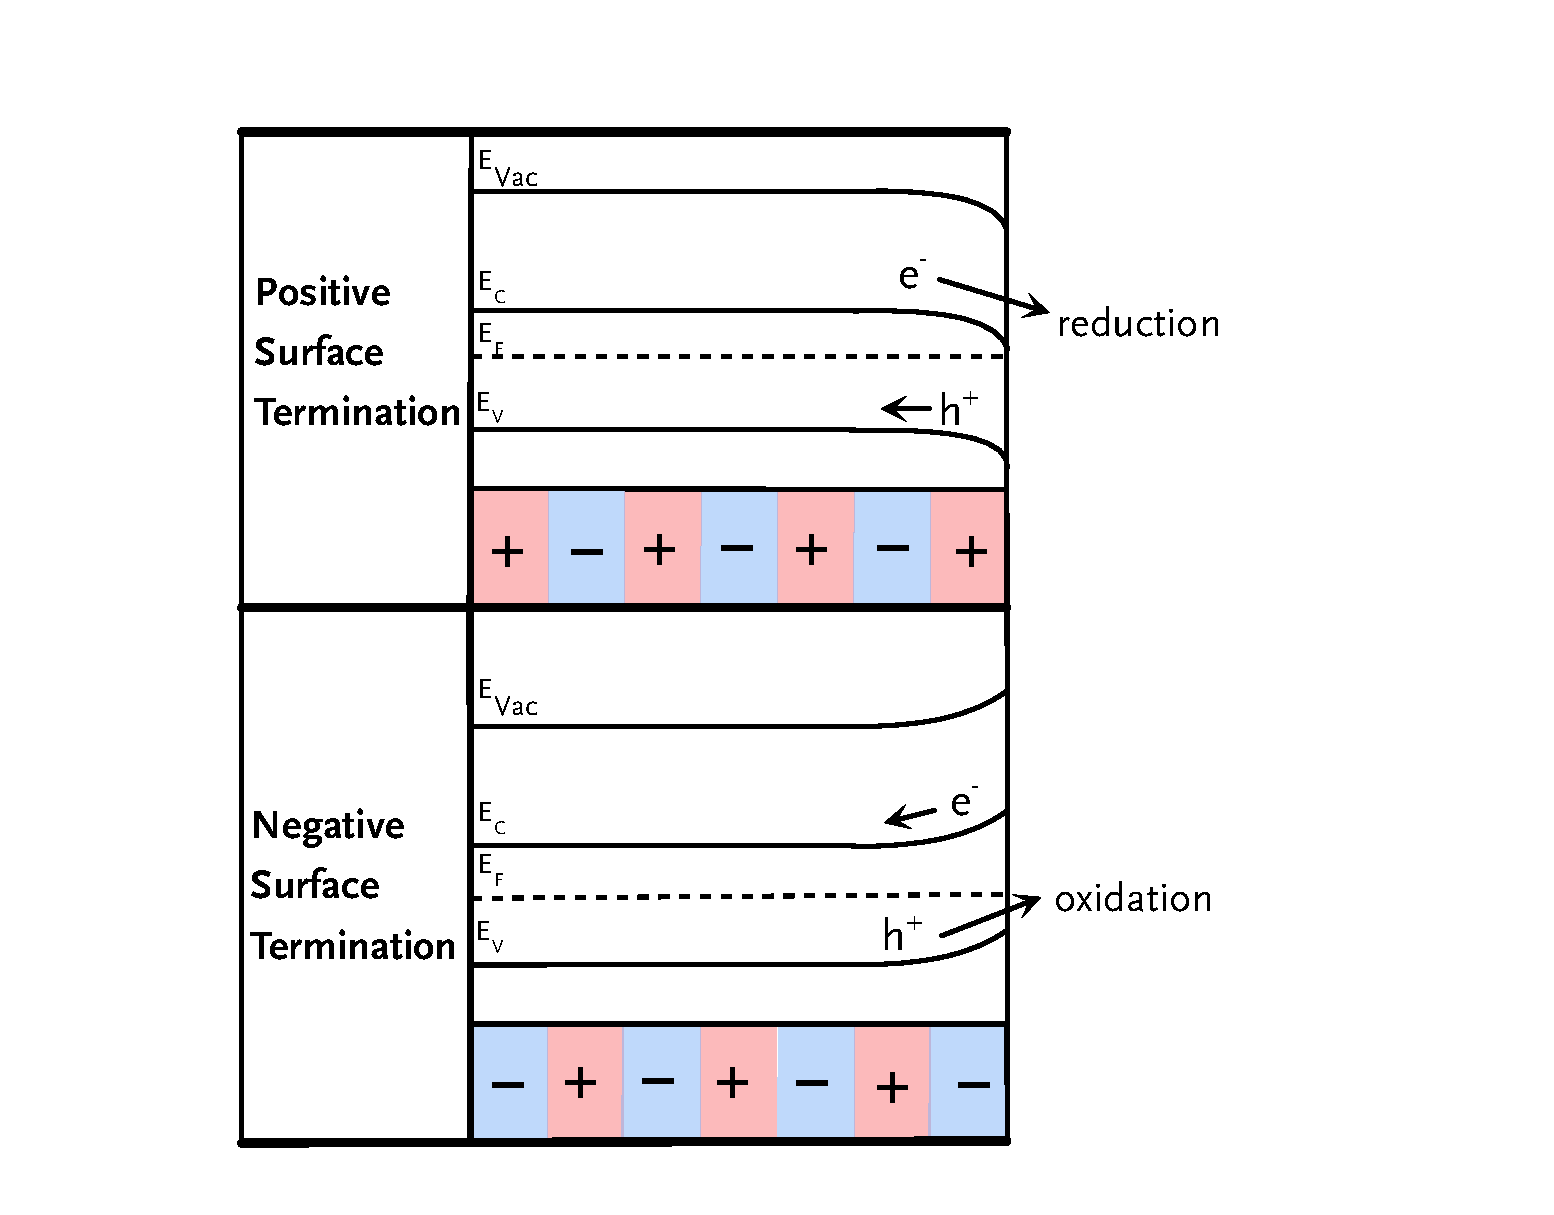
\includegraphics[width=0.8\textwidth]{polarterminations.pdf}}
	\caption[Band bending arising from polar surface terminations]{%
		Band bending at the surface of an orientation with polar surface 
		terminations. A positive surface termination bends the bands 
		downward, favoring reduction. A negative surface charge bends the 
		bands upward, favoring oxidation.}
	\label{fig:polarterminations}
\end{figure}


\section{Epitaxy}
\label{sec:background.epitaxy}


Epitaxy refers the ordered growth of new solid film phase on an existing solid material.\cite{Opel:2012ge,Herman:2004to,Hooks:2001vy} During epitaxial growth, the  film phase and orientation can be controlled through proper choice of substrate and processing conditions. The periodic lattice of the substrate drives the film to adopt a lattice with similar lattice parameters. Epitaxial film growth is an important aspect of electronic and optical technologies.

\begin{figure}
\begin{center}
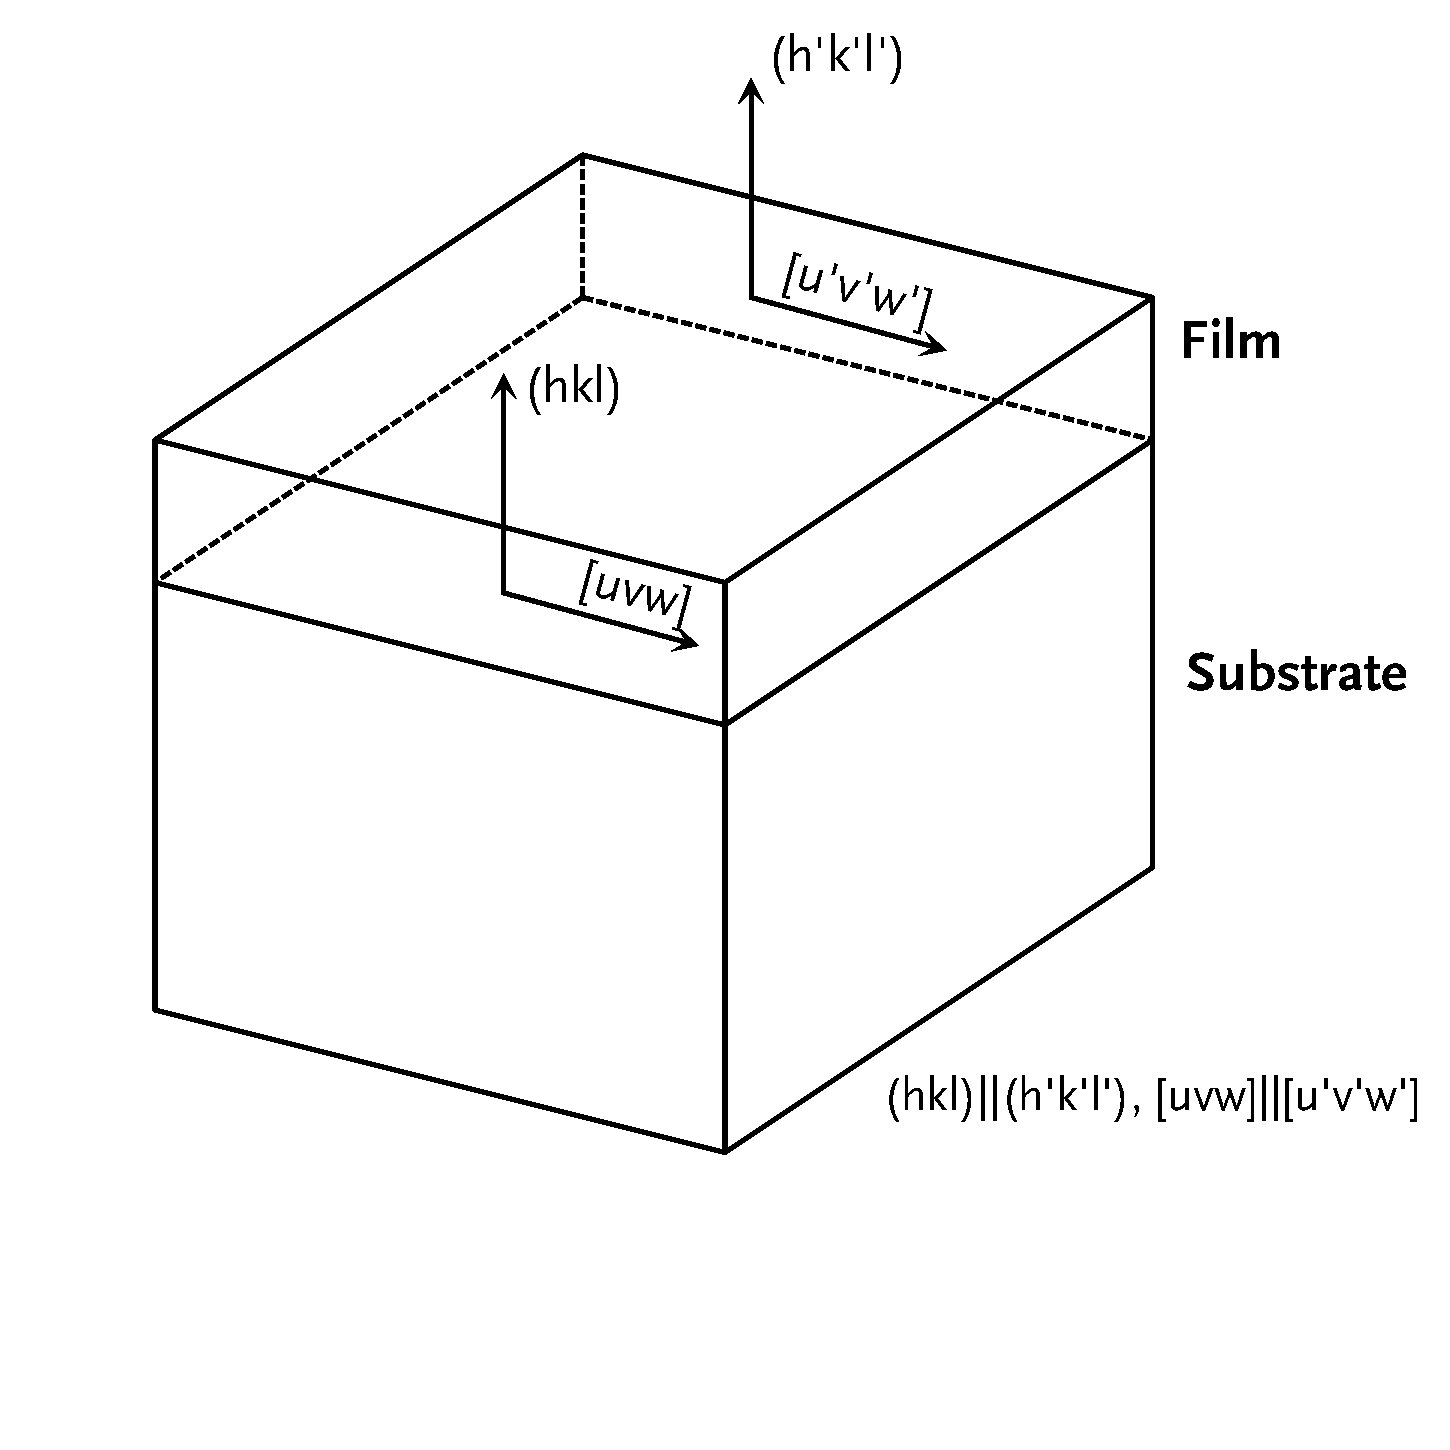
\includegraphics[width=0.7\textwidth]{epitaxy.pdf}
\caption[Orientation relationships in epitaxy]{%
	Diagram showing the sets of parallel directions that describe epitaxial 
	growth. The planes of the film and substrate parallel to the sample surface
	make up one pair. A direction within that plane makes up the second pair. }
\label{fig:epitaxy}
\end{center}
\end{figure}
%\sidefigure[Orientation relationships in epitaxy]{%
%	Diagram showing the sets of parallel directions that describe epitaxial 
%	growth. The planes of the film and substrate parallel to the sample surface
%	make up one pair. A direction within that plane makes up the second pair. 
%	\label{fig:epitaxy}
%	}{%
%	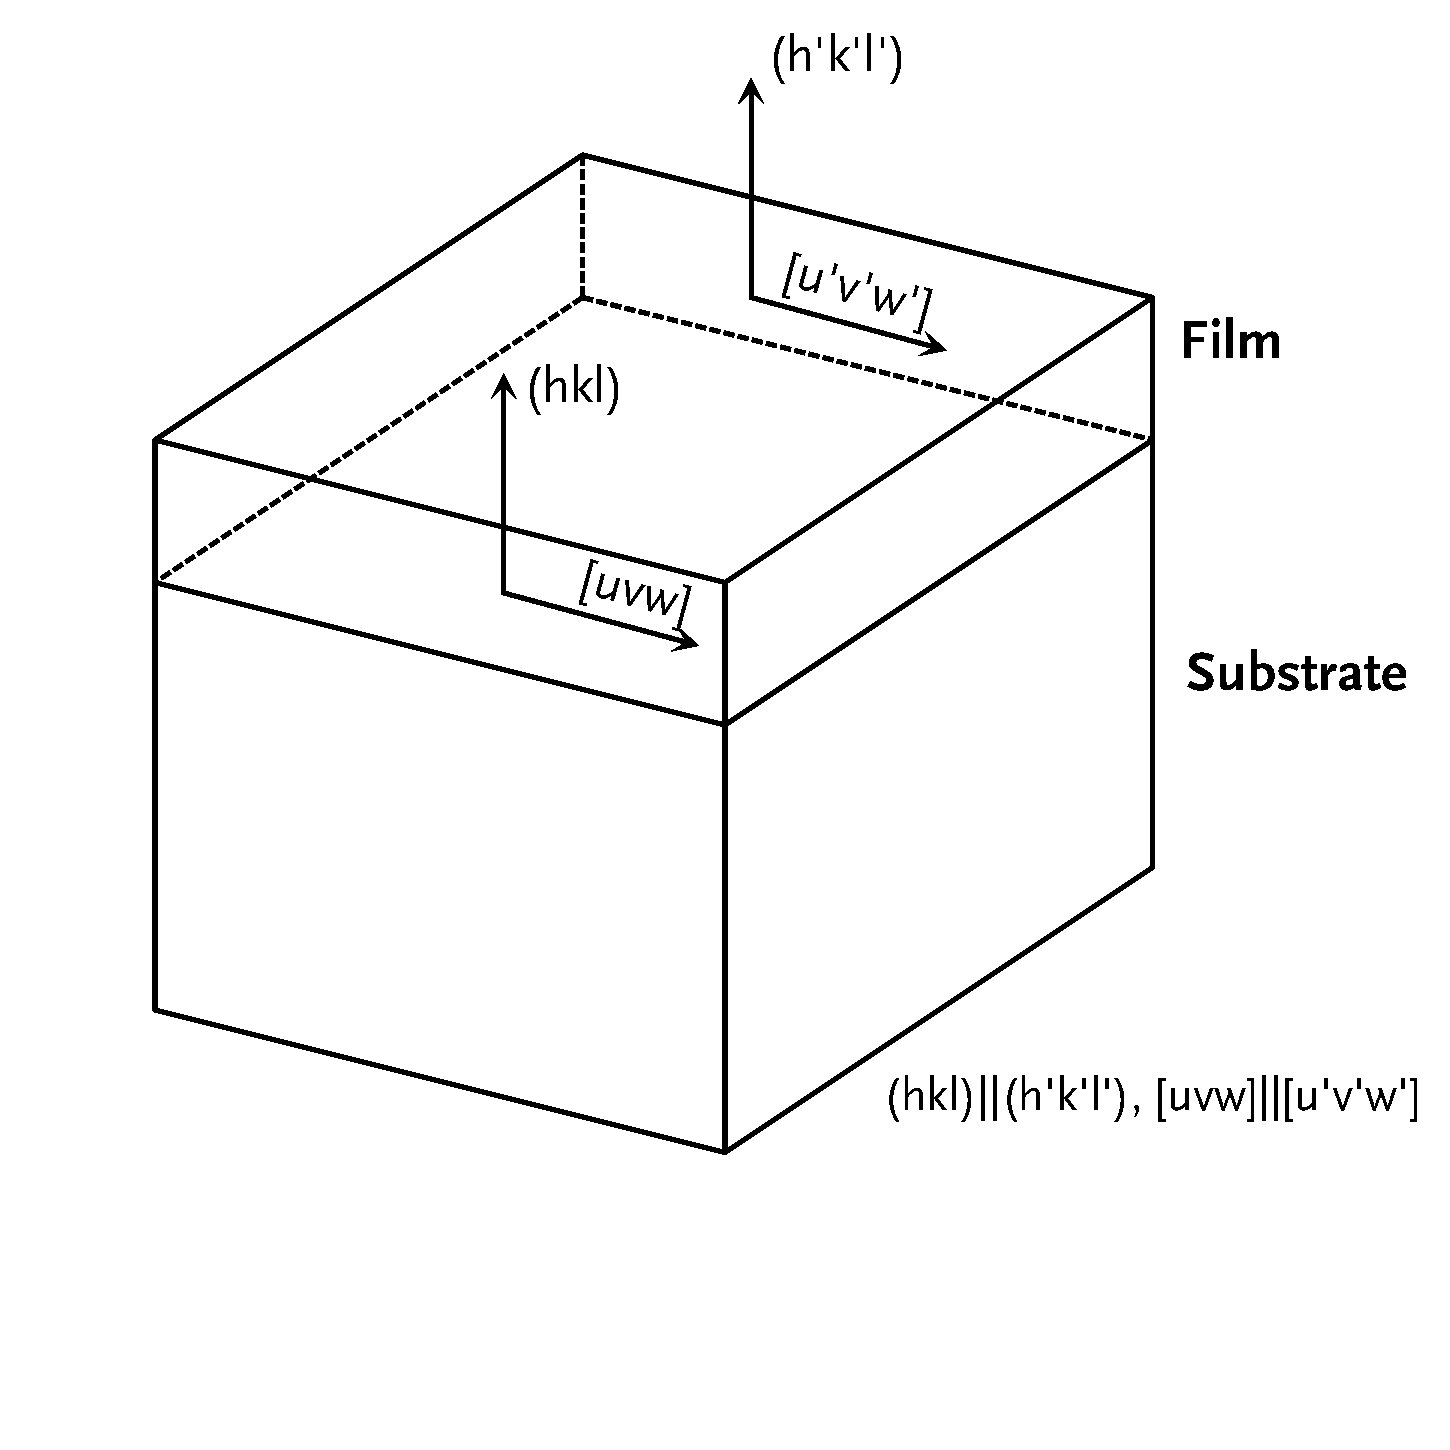
\includegraphics[width=\marginparwidth]{epitaxy.pdf}
%}{-15} % Last argument is number of lines to move up or down
Depending on the nature of the materials involved in film growth, the type of epitaxy can be termed homoepitaxy or heteroepitaxy. Homoepitaxy refers to growth of the same material as the substrate. When the film material is different from the substrate material, the process is called heteroepitaxy. For example, this document reports on heteroepitaxial hematite films grown on perovskite substrates. Epitaxial growth is characterized by a consistent orientation relationship between the film and the substrate. This relationship is described by two orthogonal pairs of parallel directions. Generally, the first pair is the set of normals to the planes parallel to the sample surface in both the film and the substrate. The second pair is two parallel directions within that plane (one in the substrate, one in the film). 

Predictions of epitaxial growth and the resulting orientation relationships typically look at a 2\textsc{D} analysis of the surface lattice parameters. If possible, the film material is energetically stabilized by forming a face and orientation that closely matches the substrate lattice parameter. The difference between the film and substrate lattice parameter is called the lattice misfit, and is given by 
\begin{equation}
f=\frac{a_{f}-a_{s}}{a_{s}},
\end{equation}
where $a_{f}$ is the film lattice parameter and $a_{s}$ is the substrate lattice parameter.\cite{Opel:2012ge} When the lattice mismatch $f$ is zero, the film lattice parameter is equal to the substrate lattice parameter and the film is unstrained. When $f$ is less than zero, the film lattice parameter is smaller than the substrate lattice parameter and an epitaxial film will exhibit tensile in plane strain and compressive out of plane strain. When the reverse is true and $f$ is greater than zero, the film experiences compressive in plane strain and tensile out of plane strain. As the film grows thicker, misfit dislocations can be introduced to the lattice, reducing the strain of the film. Above a certain thickness d$_{c}$ specific to the film-substrate system, the film is relaxed, and additional layers are generally unstrained, excepting sources of local strain such as misfit and threading dislocations. Each of these cases is illustrated schematically in \figureref{filmgrowth}.
\begin{figure}
	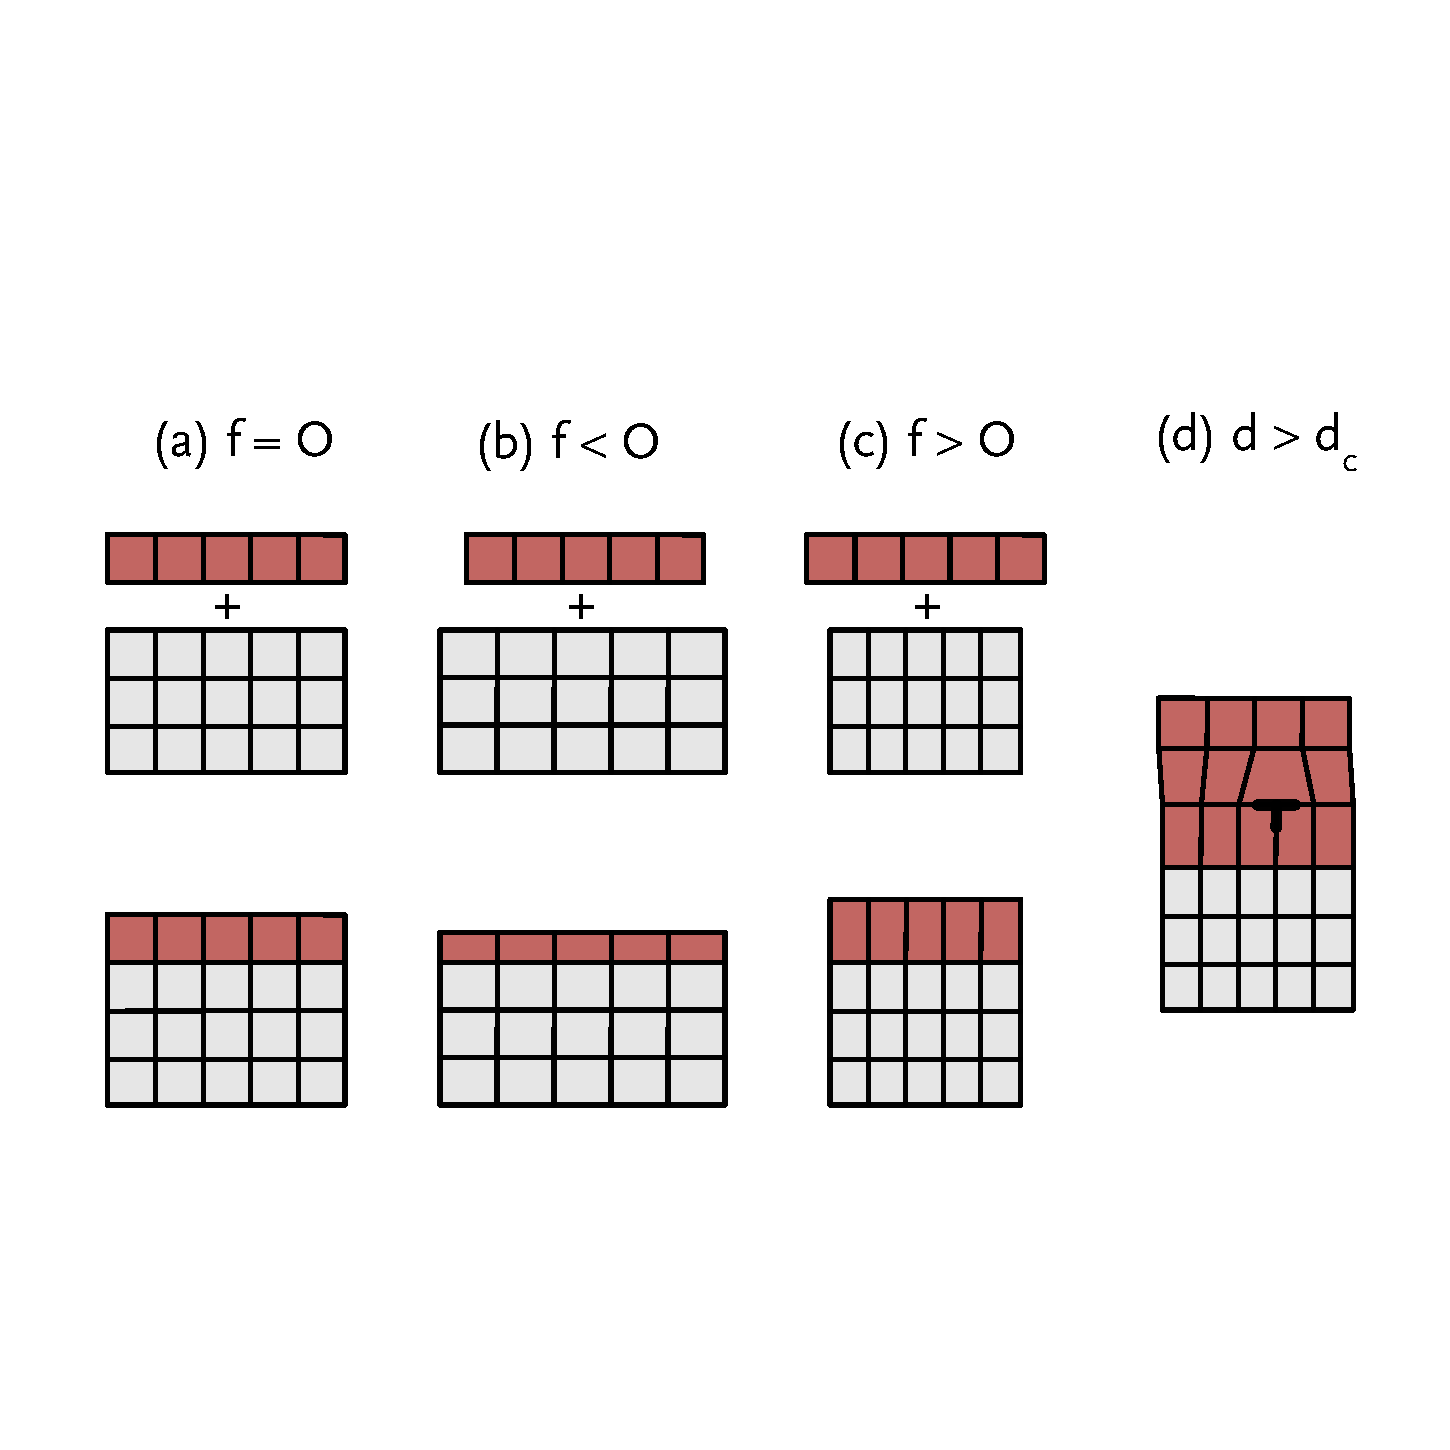
\includegraphics[width=\textwidth]{filmgrowth.pdf}
		\caption[Strain in thin film growth]{%
			(adapted from Opel\citep{Opel:2012ge}) Effect of lattice mismatch 
			on epitaxial growth and strain.
			When the film lattice parameter equals the substrate, as in (a),
			the film is unstrained. A smaller film lattice parameter (b) or
			larger film lattice parameter (c) than the substrate results in
			a strained film. (d) As the film grows thicker, dislocations appear
			in the lattice, reducing the strain state of the film.}
	\label{fig:filmgrowth}
\end{figure}

In this document, the nature of epitaxy for hematite film growth on various oxide substrates is explored. Initially, epitaxial growth was obtained on favorable substrates such as \ce{Al2O3} or (111)-oriented \ce{SrTiO3} which are isostructural or have an isostructural surface lattice respectively. Then film growth, epitaxy and orientation relationships were observed for more unconventional substrates, including (001)-oriented \ce{SrTiO3}, which has a different surface structure than \ce{Fe2O3} or polycrystalline substrates, which expose complex high index surface planes. Film growth on these high index planes, and the resulting orientation relationships are reported in this document.

\section{Crystallography}
\label{sec:background.crystallography}


Crystal structure plays an important role in the photochemical reactivity and epitaxy of oxide materials. The following sections give a brief overview of the crystallographic properties of the materials mentioned in this document.

\subsection{Hematite}
\label{subsec:background.hematite}

\begin{figure}
\centering
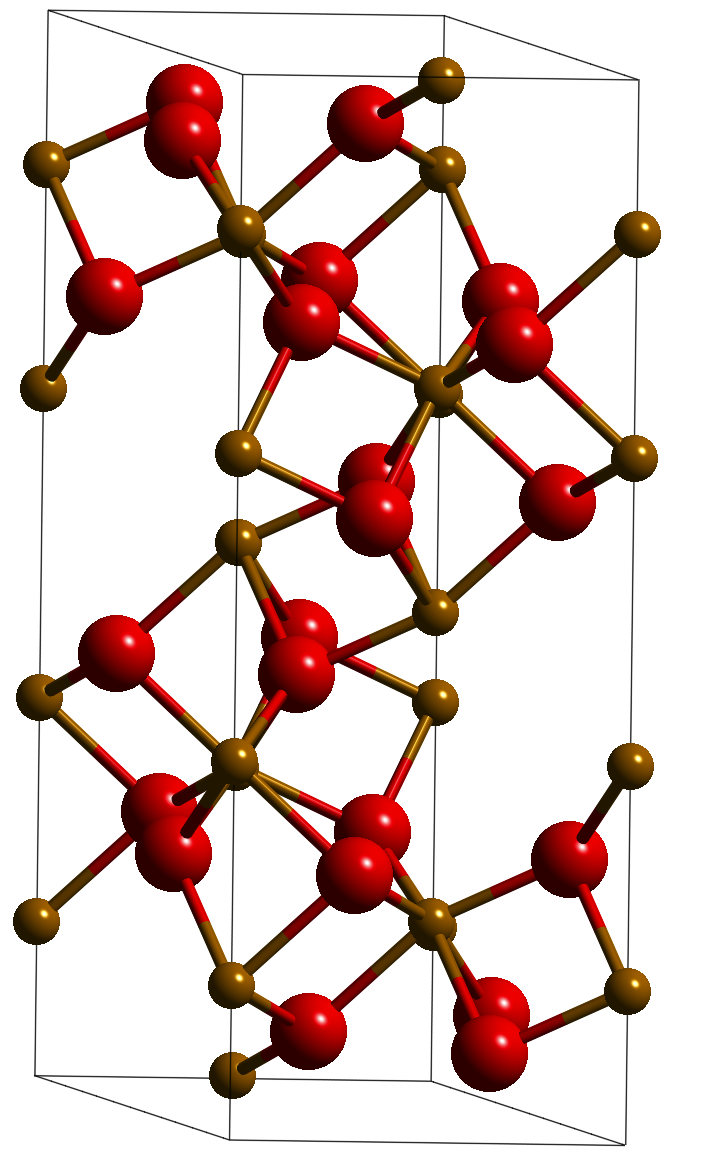
\includegraphics[width=0.4\textwidth]{hematitecell.png}
\caption[Hexagonal hematite unit cell]{%
	The hematite hexagonal unit cell. Red atoms represent oxygen, and brown atoms represent iron.  The structure is formed by hexagonal close packed oxide ions stacked along [0001] with ferric ions in two thirds of the octahedral interstices.}
\label{fig:hematitecell}

\end{figure}
%\sidefigure[Hematite hexagonal unit cell]{%
%	The hematite hexagonal unit cell. Red atoms represent oxygen, and brown atoms represent iron.  The structure is formed by hexagonal close packed oxide ions stacked along [0001] with ferric ions in two thirds of the octahedral interstices.
%	\label{fig:hematitecell}
%	}{%
%	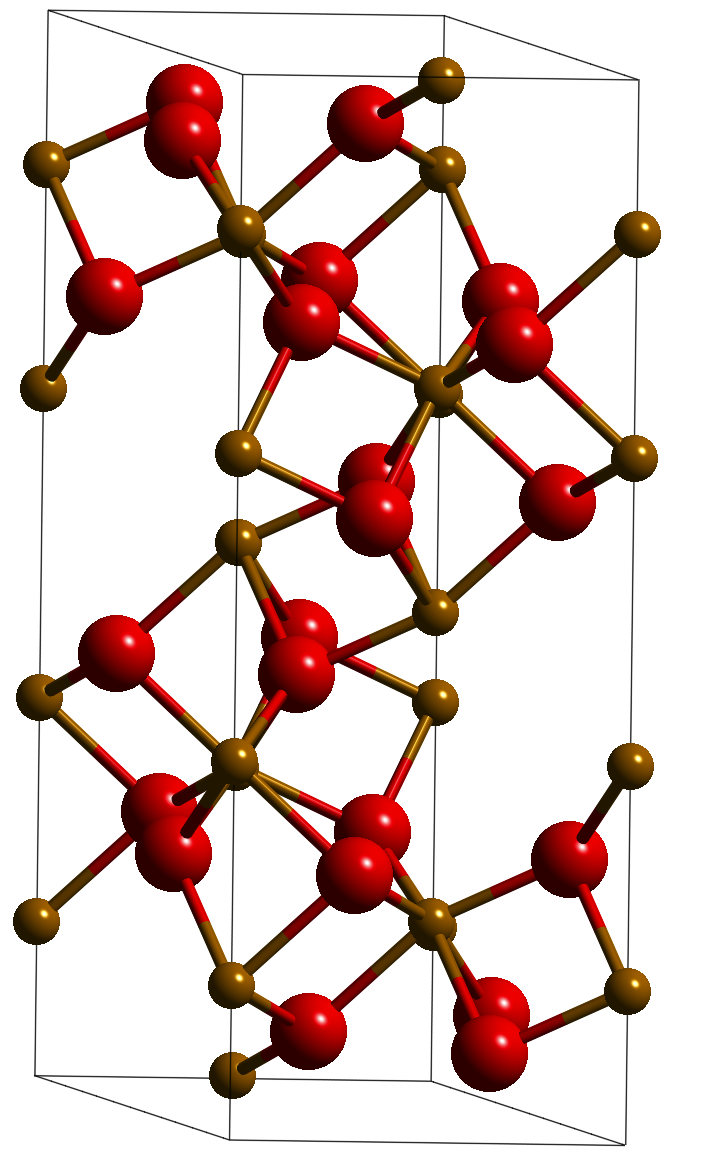
\includegraphics[width=\marginparwidth]{hematitecell.png}
%}{-18}

Hematite, \textalpha-\ce{Fe2O3}, is a promising material for use as a photolysis catalyst because it has a band gap of about 2.2~eV, which lies well into the visible spectrum.\cite{Lin:2011kw} This band gap is also larger than the minimum required to split water, 1.23~eV. Additionally, \ce{Fe2O3} is inexpensive, readily available, chemically stable in aqueous environments, and doesn't contain environmentally hazardous elements. Hematite has been widely studied for photochemical purposes,\cite{Sivula:2011cc} including as powders,\cite{GONDAL:2004df} thin films,\cite{Cao:2010dm} and as a heterojunction component.\cite{Luo:2006kg,Wang:2007fp} However, the efficiency of \ce{Fe2O3} as a photocatalyst is thought to be limited by low hole mobility and short carrier lifetimes.\cite{Sivula:2011cc} Incorporating semiconductors in heterostructures to improve photochemical activity is widely reported.\cite{Maruska:1979tr} 

In this document, the photochemical behavior of \ce{Fe2O3} films on single crystal and polycrystalline substrates is discussed. Details of \ce{Fe2O3} film growth on these substrates are also reported, including the orientation relationships between \ce{Fe2O3} films and perovskite substrates. The corundum type structure of the hematite unit cell is shown in \figureref{hematitecell}. The structure is formed by layers of hexagonal-close-packed oxygen ions stacked along the [0001] direction, with iron(III) ions in two-thirds of the octahedral interstices. This arrangement is of importance when considering the heteroepitaxy of \ce{Fe2O3} films on perovskite substrates, presented in this document. 

\subsection{Perovskites}\label{subsec:background.perovskites}

The perovskite structure is formed by many materials with the formula \ce{ABO3}, where A and B are metal cations, and the A cation is significantly larger than the B cation.\cite{Bhalla:2000ku} The cell takes the form of a cubic cell with the larger A cation sitting on the cubic P lattice sites. The smaller B cation occupies the body centered position of the cubic cell, while the O anions occupy the face centers of the unit cell. This configuration can be described as \ce{AO3} forming a cubic close packed network with B cations in one quarter of the octahedral interstices.

In addition to the prototypical cubic structures, perovskites are also found in a variety of distorted cubic lattices. Common perovskite distortions give rise to tetragonal, orthorhombic, and rhombohedral unit cells. The distortion of the unit cell gives rise to materials with many interesting properties, including ferroelectricity and ferromagnetism. Perovskite materials are widely studied\cite{Bhalla:2000ku} for applications in electronic devices,\cite{Kingon:2000wa} fuel cells,\cite{Zhu:2003jz,Jiang:2008fb} gas sensors,\cite{Fergus:2007tm} superconductivity,\cite{Murphy:1987wc} and catalysis.\cite{Lombardo:1998uv}

\subsubsection{Strontium Titanate}\label{subsubsec:background.sto}

\begin{figure}
\begin{center}
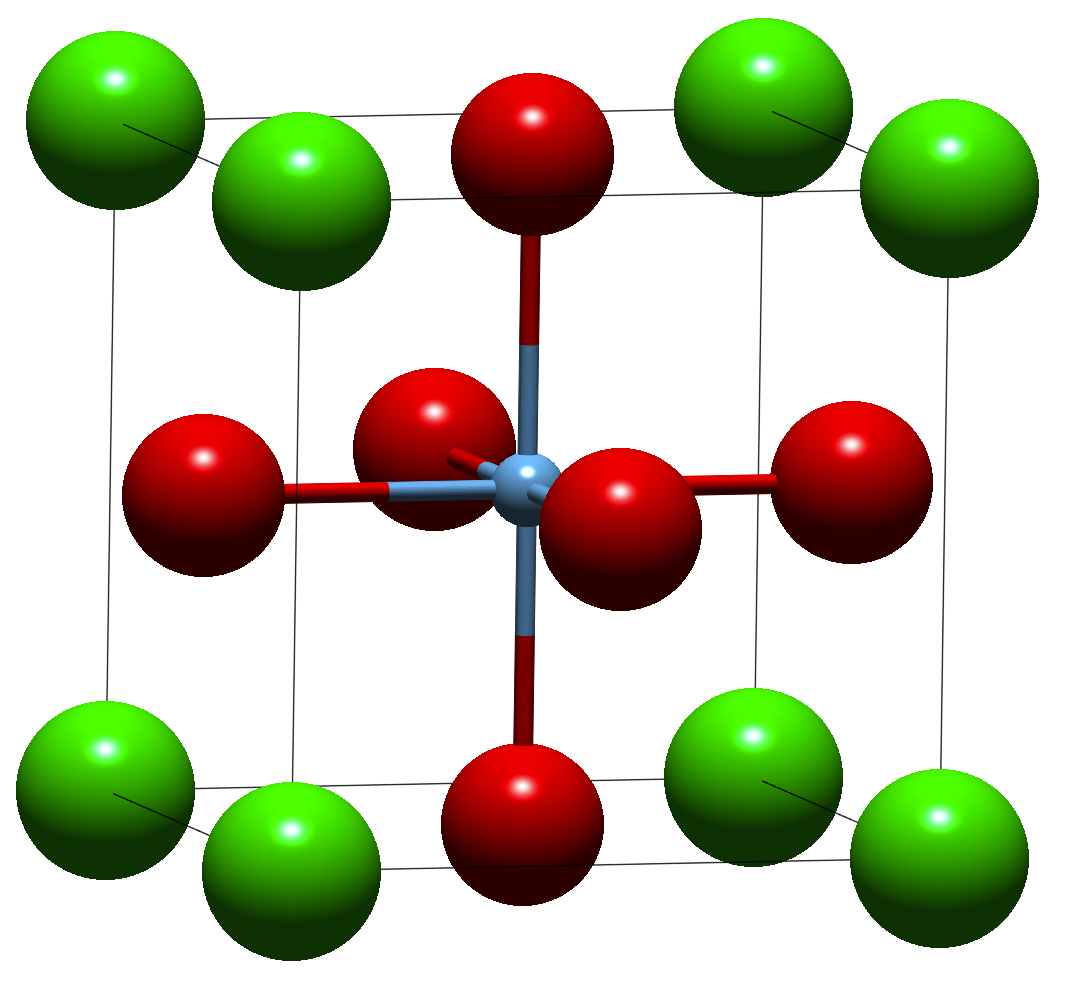
\includegraphics[width=0.4\textwidth]{stocell.png}
\caption[Cubic \ce{SrTiO3} unit cell]{%
	The cubic \ce{SrTiO3} unit cell. The cell takes the form of a 
	cubic cell with the larger Sr cation (green) sitting on the 
	cubic P lattice sites. The smaller Ti cation (blue) occupies 
	the body centered position of the cubic cell, while the O anions 
	(red) occupy the face centers of the unit cell.}
\label{fig:stocell}
\end{center}
\end{figure}
%\sidefigure[Cubic \ce{SrTiO3} unit cell]{%
%	The cubic \ce{SrTiO3} unit cell. The cell takes the form of a 
%	cubic cell with the larger Sr cation (green) sitting on the 
%	cubic P lattice sites. The smaller Ti cation (blue) occupies 
%	the body centered position of the cubic cell, while the O anions 
%	(red) occupy the face centers of the unit cell.
%	\label{fig:stocell}
%	}{%
%	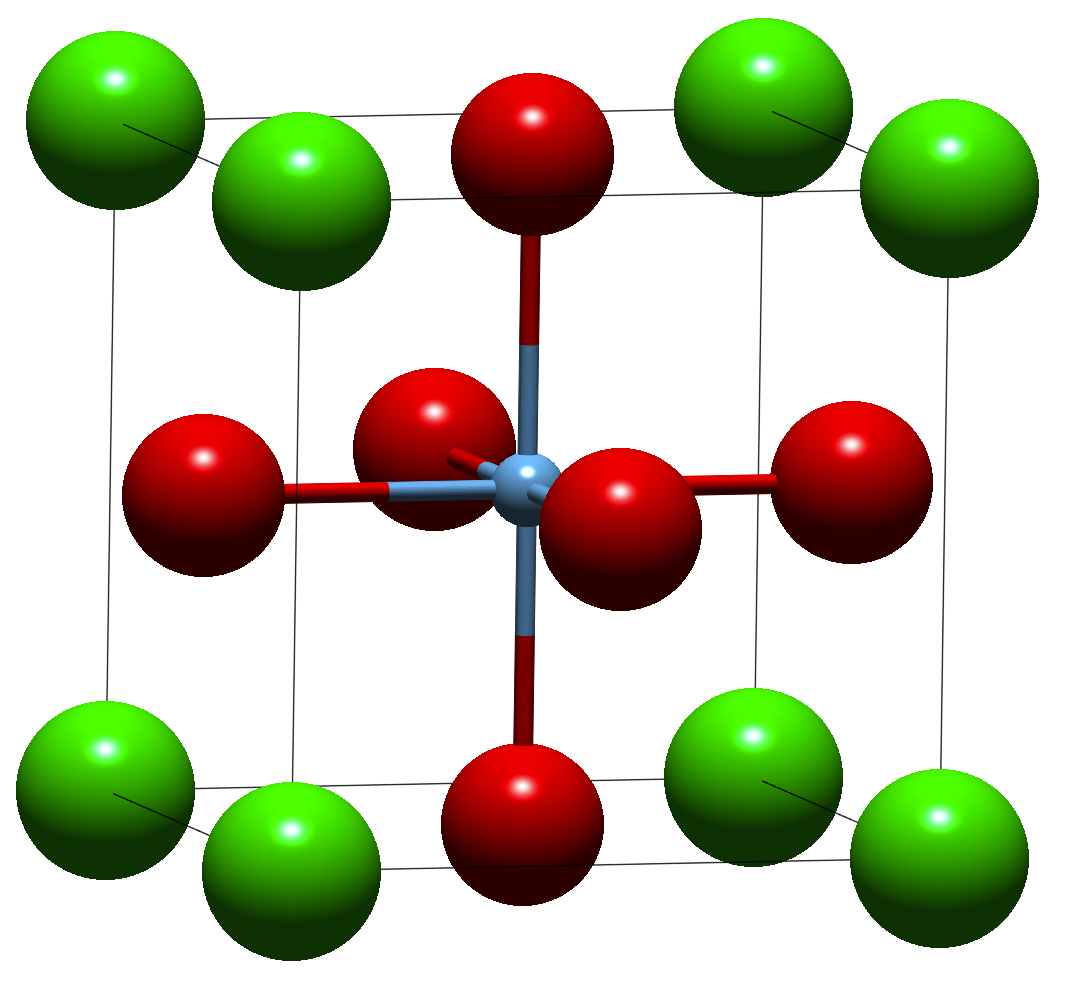
\includegraphics[width=\marginparwidth]{stocell.png}
%}{-5}

Strontium titanate, \ce{SrTiO3}, is a cubic perovskite at room temperature. It has a lattice parameter 3.905 \si{\angstrom}. The unit cell of \ce{SrTiO3} is depicted in \figureref{stocell}. At room temperature, \ce{SrTiO3} takes the form of the prototype cubic perovskite described in \sectionref{subsec:background.perovskites}, with Sr atoms on the primitive lattice sites, Ti atoms at the body center, and O atoms on the face centers of the cubic cell. The band gap of strontium titanate is 3.2~eV,\cite{Cardona:1965vw} corresponding to the ultraviolet range of the electromagnetic spectrum. In this work, \ce{SrTiO3} was selected as a material for \ce{Fe2O3} film growth on single crystal substrates. 
 
Depending on orientation, ideal \ce{SrTiO3} surfaces can be polar or nonpolar. The (001) face of strontium titanate is nonpolar, existing as neutral planes of either SrO or \ce{TiO2}. The (110) and (111) surface are polar. In the case of (110) oriented planes, possible surface terminations are \ce{SrTiO^{4+}} and \ce{O2^{4-}}. For (111) oriented surface, surface terminations are \ce{SrO3^{4-}} and \ce{Ti^{4+}}. Projections of the (001), (110), and (111) surfaces are shown in \figureref{stoterms}. The effect of substrate surface polarity on photochemical behavior of supported films is discussed later in this document.

\begin{figure}
%	\begin{whole}
	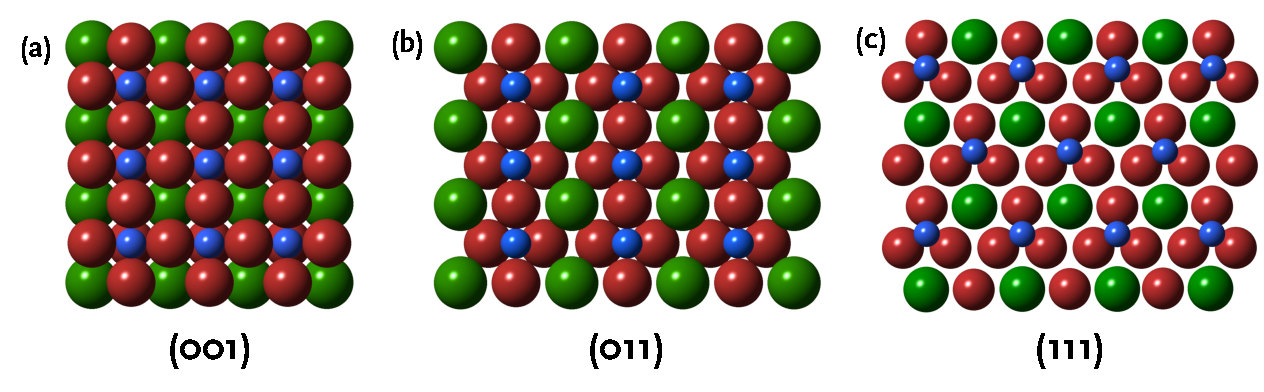
\includegraphics[width=\textwidth]{stoterms.pdf}
		\caption[Low-index \ce{SrTiO3} surface terminations]{%
			Models of the \ce{SrTiO3} (001), (011), and (111) surface. 
			Red, green, and blue represent oxygen, strontium, and oxygen 
			atoms respectively. The (001) surface is terminated by neutral 
			\ce{TiO2} and \ce{SrO} terminations. The (011) and (111) 
			terminations are polar. The (011) surface is either \ce{SrTiO} 
			or \ce{O2} terminated and the (111) surface is terminated by 
			either Ti or \ce{SrO3} layers.}
	\label{fig:stoterms}
%	\end{whole}
\end{figure}

%\subsubsection{Barium Titanate}
%\label{subsubsec:background.bto}
%
%\sidefigure[AFM micrograph of a \ce{BaTiO3} surface]{%
%	AFM micrograph of a \ce{BaTiO3} surface showing 180\si{\degree} 
%	and 90\si{\degree} domain boundaries.
%	\label{fig:btosurface}
%	}{%
%	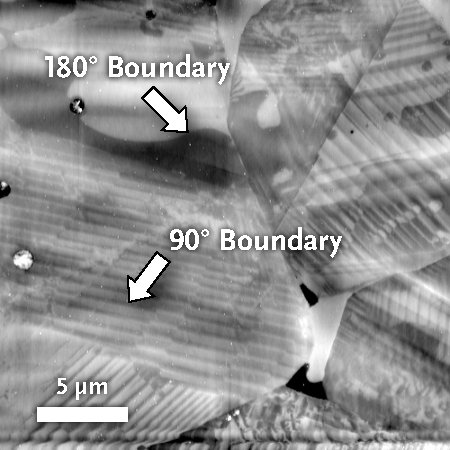
\includegraphics[width=\marginparwidth]{btosurface.pdf}
%}{-1}
%
%\ce{BaTiO3} is a tetragonally distorted perovskite with a band gap of 3.2~eV. \ce{BaTiO3} is typically an n-type semiconductor, owing to presence of oxygen vacancies. When cooled below its Curie temperature of 120 \si{\degreeCelsius}, the unit cell shifts from cubic to tetragonal symmetry, slightly elongating along the [001] direction. The tetragonal unit cell has lattice parameters of a = 3.98 \si{\angstrom} and c = 4.03 \si{\angstrom} at room temperature.\cite{ForsberghJr:1949vl,Heywang:1971uv} This transition is paraelectric-to-ferroelectric, giving rise to ferroelectric polarization along the c-axis. The spontaneous polarization Ps at room temperature is 26 \si{\micro\coulomb\per\cm\squared}, and exists along the elongated [001] direction. This phase transition and resultant unit cell is shown in \figureref{btocell}. The figure shows how the ferroelectric polarization arises from the distortion of the Ti--O octahedra. 
%
%\begin{figure}
%	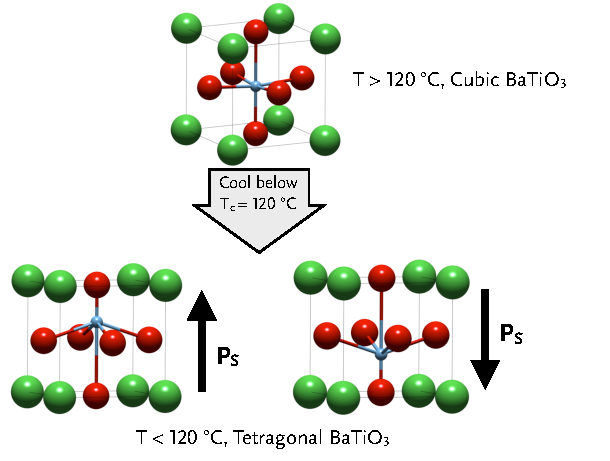
\includegraphics[width=\textwidth]{btocell.pdf}
%	\caption[\ce{BaTiO3} ferroelectric phase transition]{%
%		The cubic \ce{BaTiO3} unit cell transitioning to the 
%		ferroelectric tetragonal phase. The distortion of the 
%		Ti--O octahedra is exaggerated in this diagram.}
%	\label{fig:btocell}
%\end{figure}
%
%In this work, \ce{BaTiO3} is used as a polycrystalline substrate for \ce{Fe2O3} film growth. As discussed earlier in the section on ferroelectricity, bulk specimens of \ce{BaTiO3} contain numerous ferroelectric domains. The elongated [001] direction of the unit cell is defined to be the direction of positive ferroelectric polarization. This crystal direction can exist in the $\pm$x, $\pm$y, or $\pm$z direction.\cite{ForsberghJr:1949vl} This constraint on the direction of ferroelectric polarization gives rise to two types of domain boundaries, 90\si{\degree} and 180\si{\degree} boundaries.\cite{Anonymous:7uC1r_sG} The angle refers to the change in direction of polarization when crossing the boundary. 90\si{\degree} boundaries are confined to (110) planes and intersect the surface at straight lines. 180\si{\degree} planes are not confined to a single crystal habit, and so appear as curved lines. \figureref{btosurface} shows an AFM micrograph of a polished \ce{BaTiO3} surface, with 90\si{\degree} and 180\si{\degree} domains identified. The domains of \ce{BaTiO3} have a strong effect on the photochemical activity of \ce{TiO2} films supported on \ce{BaTiO3} substrates. The effect of these domains on the photochemical activity of \ce{Fe2O3} is reported in this document. 


\subsubsection{Bismuth Ferrite}
\label{subsubsec:background.bfo}

\begin{figure}
\begin{center}
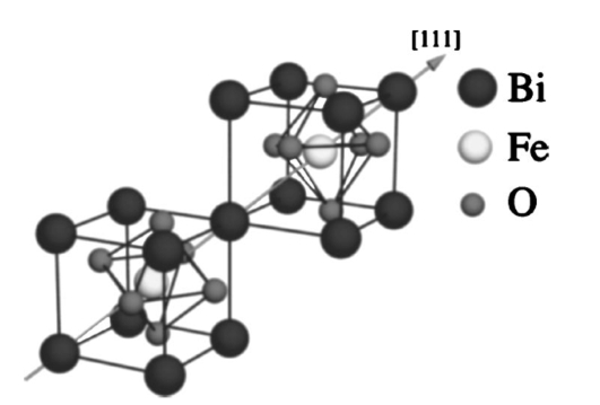
\includegraphics[width=0.6\textwidth]{bfocell.pdf}
\caption[Pseudo-cubic \ce{BiFeO3} unit cell]{%
	Pseudo-cubic \ce{BiFeO3} unit cell, showing rhombohedral [111] 
	distortion and resulting ferroelectric polarization.\cite{Catalan:2009ca}}
\label{fig:bfocell}
\end{center}
\end{figure}
%\sidefigure[Pseudo-cubic \ce{BiFeO3} unit cell]{%
%	Pseudo-cubic \ce{BiFeO3} unit cell, showing rhombohedral [111] 
%	distortion and resulting ferroelectric polarization.\cite{Catalan:2009ca}
%	\label{fig:bfocell}
%	}{%
%	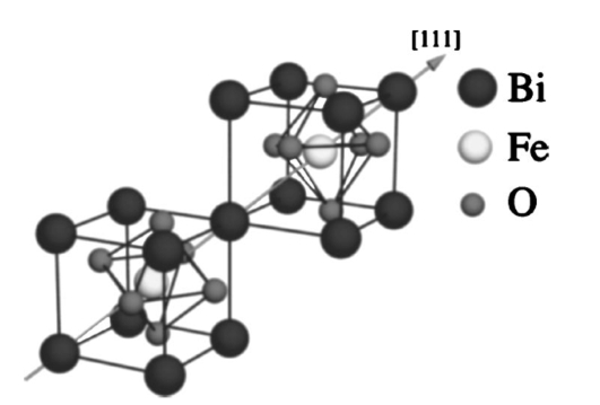
\includegraphics[width=\marginparwidth]{bfocell.pdf}
%}{-11}

Bismuth ferrite, \ce{BiFeO3}, is ferroelectric, rhombohedrally distorted perovskite with a Curie temperature of \texttildelow830-850 \si{\degreeCelsius}.\cite{Kornev:2007jr,Catalan:2009ca,Anonymous:htMDB4Eh,Miao:2008fz} The perovskite unit cell has the lattice constants $\text{a}_{\text{Rh}}$~=~3.965~\si{\angstrom} and $\text{\textalpha}_{\text{Rh}}$~=~89.4\si{\degree}.\cite{Kubel:1990kd} Because the rhombohedral distortion is so small ($\text{\textalpha}_{\text{Rh}}$~=~89.4\si{\degree} versus 90\si{\degree} for a cubic cell), crystal directions and planes are typically referenced using the pseudocubic perovskite cell rather than the more complex rhombohedral or hexagonal systems.  The pseudocubic unit cell is depicted in \figureref{bfocell}. Bulk \ce{BiFeO3} is a p-type oxide semiconductor with reported band gaps of 2.3~eV to 2.8~eV.\cite{Ihlefeld:2008hl,Clark:2007bt,Kumar:2008fr} The p-type conductivity arises from the loss of volatile bismuth during synthesis, resulting in cationic vacancies in the crystal lattice. 

The ferroelectric polarization vector is observed along the pseudocubic <111> family of directions.\cite{Catalan:2009ca} This gives rise to three possible types of domain walls: 180\si{\degree}, 109\si{\degree}, and 71\si{\degree}. 180\si{\degree} walls separate domains with antiparallel polarization vectors, for example, [111] and [\={1}\={1}\={1}]. If two of the components of the polarization vector are reversed across the boundary, it is a 109\si{\degree} wall, and if only one component is reversed, the boundary is a 71\si{\degree} wall. Equilibrium domain walls are constrained to certain orientations. 71\si{\degree} walls exist parallel to {110} planes, 109\si{\degree} walls parallel to \{100\} planes, and 180\si{\degree} walls on any plane containing the polarization vectors separated by the boundary.\cite{Streiffer:1998vt}

In contrast to \ce{BaTiO3}, for which spatially selective reactivity has been observed and characterized, \ce{BiFeO3} has a band gap in the visible spectrum, is a p-type semiconductor, and has <111> type ferroelectricity. The spatially-selective photochemical properties of \ce{BiFeO3}, taking into account these differences, were studied and are reported in this document.


		% !TEX root = base.tex 


\chapter{Experimental Overview}
\label{ch:experimental}


\chintro{The purpose of this section is to provide an overview of the fabrication and
characterization methods presented in this document. The main methods of sample
fabrication covered in this chapter are solid state synthesis of polycrystalline ceramics
and pulsed laser deposition of thin films. Characterization methods include microscopy,
thin film phase and orientation characterization, and characterization of photochemical
activity.}


\section{Fabrication Methods}
\label{sec:exp.fabrication}


\subsection{Solid State Synthesis}
\label{subsec:exp.solidstate}


Ceramic pellets were fabricated for use as polycrystalline substrates for film deposition.
By using polycrystalline substrates, photochemical properties and film growth could be
examined as a function of substrate orientation. In many cases, film growth occurs
epitaxially across the entirety of a single substrate grain. The random texture of the
substrate allows for measurement of properties across all possible orientations. As
compared to growth on single crystals, where only low index orientations are typically
available, this provides a much more diverse set of orientation conditions for
examination. 

All polycrystalline substrates and deposition targets were fabricated using a conventional
solid state synthesis route. Starting powers of metal oxides or carbonates were measured
in the correct stoichiometric proportions for the desired ceramic phase. Specific powders
and purities are listed in the sintering recipes contained in Table
\ref{tab:sinteringrecipe}.
 
\begin{table} 

	\begin{center}
	\footnotesize
	\begin{tabular}{llrrrrrrrrr}


		\multicolumn{1}{c}{Material}&
		\multicolumn{2}{c}{Starting Powder} &  
		\multicolumn{2}{c}{Reaction Step} &  
		\multicolumn{2}{c}{Burnoff} &  
		\multicolumn{2}{c}{Densification} &  
		\multicolumn{2}{c}{Grain Growth}  \\	

		\cmidrule(lr){1-1}
		\cmidrule(lr){2-3}
		\cmidrule(lr){4-5}
		\cmidrule(lr){6-7}
		\cmidrule(lr){8-9}
		\cmidrule(lr){10-11}
		
   		\ce{Fe2O3} &
		\ce{Fe2O3} &
	 	99.945\% &
		\multicolumn{2}{c}{---} &
		\SI{600}{\degreeCelsius} &
		\SI{12}{\hour}  &
		\SI{1200}{\degreeCelsius} &
		\SI{12}{\hour}  &
		\multicolumn{2}{c}{---} \\[9pt]

   		\ce{SrTiO3} &
		\ce{SrTiO3} &
	 	99.97\% &
		\multicolumn{2}{c}{---} &
		\SI{900}{\degreeCelsius} &
		\SI{10}{\hour}  &
		\SI{1360}{\degreeCelsius} &
		\SI{10}{\hour}  &
		\SI{1470}{\degreeCelsius} &
		\SI{3}{\hour}\\[9pt]
				
%   		\ce{BaTiO3} &
%		\ce{BaTiO3} &
%	 	99.97\% &
%		\multicolumn{2}{c}{---} &
%		\SI{900}{\degreeCelsius} &
%		\SI{10}{\hour}  &
%		\SI{1230}{\degreeCelsius} &
%		\SI{10}{\hour}  &
%		\SI{1360}{\degreeCelsius} &
%		\SI{3}{\hour}\\[9pt]

   		\ce{BiFeO3} &
		\ce{Bi2O3} &
	 	99.99\% &
		\SI{650}{\degreeCelsius} &
		\SI{6}{\hour}  &
		\SI{600}{\degreeCelsius} &
		\SI{12}{\hour}  &
		\SI{750}{\degreeCelsius} &
		\SI{12}{\hour}  &
		\SI{850}{\degreeCelsius} &
		\SI{3}{\hour}\\
		
		&
		\ce{Fe2O3}&
		99.945\%&
		&
		&
		&
		&
		&
		&
		&
		\\
		
	\end{tabular}
	\end{center}
   	\caption[Sintering recipes for polycrystalline pellets]{%
   		Sintering recipes for polycrystalline pellets used in this work. All starting
powders were purchased from Alfa Aesar (Ward Hill, MA).}
   	\label{tab:sinteringrecipe}

\end{table}
These powders were ball milled in ethanol using yttria-stabilized zirconia (\abbr{YSZ})
grinding media (Inframet Advanced Materials, Manchester, \abbr{CT}). The powders were
typically ball milled overnight to ensure complete mixing of the starting powders. The
slurry was placed in a drying oven to drive off ethanol. The dry powders were placed in an
alumina crucible and calcined to promote reaction of the starting powders into the desired
final phase. After this reaction step, the powders were ball milled overnight in ethanol
again. Before ball milling, a small amount (typically 1-2~wt\%) of polyethylene glycol
(\abbr{PEG}, \abbr{MW}8000, ) was added to act as a binder.  After ball milling, the
powders were dried as before. % Add the company to PEG

Pellets were formed of the dried powders under uniaxial loads in a stainless steel die.
The diameter of the die was approximately \SI{1}{\centi\meter} for polycrystalline
substrates and \SI{2.5}{\centi\meter} for film growth targets. The sides of the die were
coated with a saturated solution of stearic acid in ethanol to act as a lubricant. A small
amount of powder was added to the die. The die was placed on a manual hydraulic press  and
subjected to a load of 5000~pounds. The applied load was immediately released, and the
pellet was ejected from the die. Pellets were placed in an alumina crucible, with a small
amount of excess powder forming a barrier between the crucible and the pellets. Additional
pellets were stacked, until the crucible was full or the desired number of pellets was
reached. Any excess powder was loosely poured on top of the pellets to reduce loss of
volatile elements to the atmosphere during sintering.

The crucible was placed in the furnace, and heated in air according to the desired
sintering program. The same furnace was used to fabricate all specimens in this work. The
furnace allows a programmable series of sintering steps. Typically, the furnace was held
first at a low temperature to burn off organic materials in the pellet. Next, the
temperature was increased to a point where densification and sintering occur. Finally, the
temperature was increased to promote grain growth. Depending on the material, one or more
of these steps may be omitted from the synthesis procedure.

After the samples were cooled to room temperature, they were removed from the crucible.
Substrates were lapped flat and polished to provide a high quality surface for film
growth, electron backscatter diffraction analysis, and photochemical reaction. All
polishing was done using an autopolisher (Logitech, \abbr{UK} Scotland). Samples were
affixed to glass substrates using melted wax (Logitech), which were held to a polishing
jig with a vacuum. Lapping was performed using a steel plate and \SI{9}{\micro\meter}
alumina slurry (Buehler, Lake Bluff, \abbr{IL}). Both sides of each sample were lapped
flat, ensuring that the sides were parallel and had a uniform flat surface. Deionized
water was used to remove lapping residue. After both sides were flat, one side was
polished. For final polishing,{ }\SI{0.01}{\micro\meter} colloidal silica (MasterMet 2,
Buehler) was used with a polyurethane plate. The slightly basic nature of the colloidal
silica results in a chemomechanical polishing process, ensuring a smooth, flat surface.
Polishing times varied for each material, but were on the order of \texttildelow30~minutes
for each sample. Each sample was examined using optical microscopy to verify the removal
of surface scratches and roughness. After polishing, the pellets were annealed a final
time to heal surface damage from polishing and thermally etch the grain boundaries. 


\subsection{Pulsed Laser Deposition}
\label{subsec:exp.pld}


Pulsed laser deposition (\abbr{PLD}) was used to fabricate the thin films discussed in
this document. Benefits of \abbr{PLD} benefits include the ability to deposit
stoichiometric oxides, rapid and simple changeout of target materials, precise control of
film thickness, and easy control of deposition conditions.\cite{Chrisey:1994ta} A pulsed
laser deposition system consists of a high power pulsed ultraviolet laser, a focusing
optic system, and a vacuum chamber including an optical window for the laser, a target
holder, and a substrate holder and heater. A schematic of the system used in this work is
presented in Figure \ref{fig:pldsetup}.
\begin{figure}[b]
	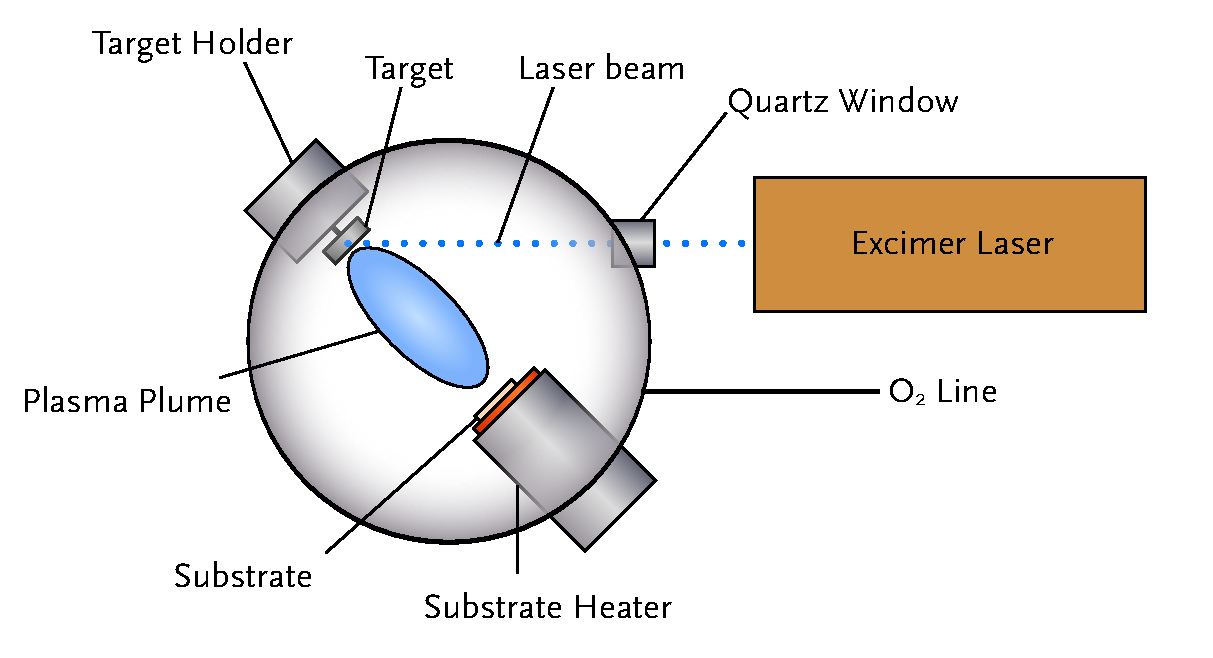
\includegraphics[width=\textwidth]{pldsetup.pdf}
	\caption[Schematic of pulsed laser deposition apparatus]{%
		Schematic of the pulsed laser deposition apparatus used in 
		this work, showing the location of the substrate and target, 
		and their relation to the pulsed laser beam.}
	\label{fig:pldsetup}
\end{figure}
The laser  beam enters the vacuum chamber through the quartz optical window. The beam is
aligned at a \SI{45}{\degree} angle from the target surface. The focused beam rapidly
heats the target material in a process called ablation. The high incident flux and energy
of the laser causes the formation of a plasma plume. The plume forms in a direction normal
to the surface of the target. The plume expands in the chamber, its shape and size
dependent on the energy of the laser pulse and the pressure of the process gas inside the
chamber. The substrate is affixed to a heater located parallel to the target material. As
the plume reaches the substrate, film nucleation and growth occurs. Each laser pulse
delivers a relatively consistent amount of film material to the substrate, and resulting
in typical growth rates on the order of \SI{0.01}{\nano\meter\per\pulse}. By determining
the growth rate via measurements of film thicknesses for films deposited with known
numbers of pulses, accurate values of film thicknesses can be obtained.

The key parameters controlled during pulsed laser deposition are the substrate
temperature, the pressure and composition of the process gas in the chamber, the
target-substrate distance, the laser energy, and the laser repetition rate. The substrate
temperature can strongly affect the crystallinity and phase of the resultant film. Higher
substrate temperature increases the crystallinity of the film, and increases the
likelihood of epitaxial growth.\cite{Francis:2004cf} The laser energy and repetition rate
combine to affect the rate of arrival of material to the substrate. At higher laser
energies, a greater amount of material is ablated from the target. If the laser repetition
rate is increased, the time between pulses is reduced, and the rate of ablated material
reaching the substrate is increased. By increasing or decreasing these values, kinetically
or thermodynamically stabilized film phases can be deposited. The substrate-target
distance affects the growth rate of the material. If the substrate is placed closer to the
target, a larger portion of the plasma plume is directed at the substrate, increasing the
growth rate. 

The process gas in the chamber during deposition and cooling affects film phase,
composition, and growth rate. A dynamic oxygen atmosphere is commonly used during
deposition to ensure the formation of oxide films. By varying the pressure of the oxygen
during deposition, various stoichiometric oxide compositions can be created from a single
metal or metal oxide target. Under high oxygen partial pressures, the formation of the
more highly oxidized material is favorable. The reverse is true under vacuum or low oxygen
pressures. In the scope of this work, a higher oxygen pressure during deposition creates
favorable conditions for the formation of the desired \ce{Fe2O3} phase rather than
\ce{FeO} or \ce{Fe3O4}. The atmosphere during post deposition annealing and cooling also
can affect the phase of the resulting film.

A commercially available pulsed laser deposition system from Neocera (Beltsville,
\abbr{MD}) was used for all film growth presented in this document. A KrF excimer laser
(Coherent, Santa Clara, \abbr{CA}) with a wavelength of \SI{248}{\nano\meter} was used for
ablation. Unless otherwise noted, substrates were cleaned ultrasonically in acetone and
then methanol. Substrates were affixed to the substrate heater with silver paint. The
substrate-target distance was fixed at \SI{6}{\centi\meter} for all depositions. The
chamber was evacuated to a base pressure of $10^{-5}$~\si{\torr} before substrate heating
began. Substrate heating and cooling rates were in the range of
20-30~\si{\degreeCelsius\per\minute}, as regulated by a programmable temperature
controller. While the substrate was heating, the target surface was cleaned by ablating it
with the laser. During target cleaning, a shield was kept in between the target and the
substrate to block the plume from reaching the substrate. Once deposition temperature was
reached, a dynamic oxygen atmosphere was established by flowing oxygen through the chamber
with the vacuum pump in operation. The shield between the target and substrate was
removed, and the target was hit with a predetermined number of laser pulses to deposit the
film. Immediately after deposition was completed, the chamber was sealed, and a static
oxygen atmosphere was introduced into the chamber while the substrate cooled. Growth
rates, laser energy, repetition rate, substrate temperature, and oxygen pressures were
controlled across all film depositions in this document. Table \ref{tab:pldparameters}
lists the values used. 
\begin{table} \small
\begin{center}
	\begin{tabular}{ll}

		Parameter &  
		Typical Value   \\
		
		\cmidrule(lr){1-1}
		\cmidrule(lr){2-2}
		
   		Substrate Temperature & 
		800~\si{\degreeCelsius} \\
		
  		Laser Energy & 
		160~\si{\milli\joule\per\pulse}  \\
		
		&
		(2~\si{\joule\per\centi\meter\squared}) \\
		
		Laser Rep Rate & 
		10~\si{\hertz} \\
		
		Deposition Gas Pressure & 
		200~\si{\milli\torr} \\
		
		Annealing Gas Pressure & 
		200~\si{\torr} \\
		
		Target Composition & 
		\textalpha-\ce{Fe2O3} \\
		
		Growth Rate & 
		0.01~\si{\nano\meter\per\second} \\

	\end{tabular}
	\end{center}
  	\caption[Experimental parameters for \ce{Fe2O3} film deposition]{%
		Experimental parameters for the deposition of \ce{Fe2O3} films. 
		These parameters were consistant across all depositions in this 
		document.}
	\label{tab:pldparameters}
\end{table}

The values used reflect conditions that produced the desired film results. Initial values
were selected based on typical values for users of this \abbr{PLD} chamber. Once films of
the desired phase were obtained, growth parameters were not further optimized. The only
variable altered from film to film was the numbers of pulses, which was varied to control
the resulting thickness of the deposited film.


\section{Characterization Methods}
\label{sec:exp.characterization}


\subsection{Marker Reactions}
\label{subsec:exp.markerreactions}

\begin{figure}
\begin{center}
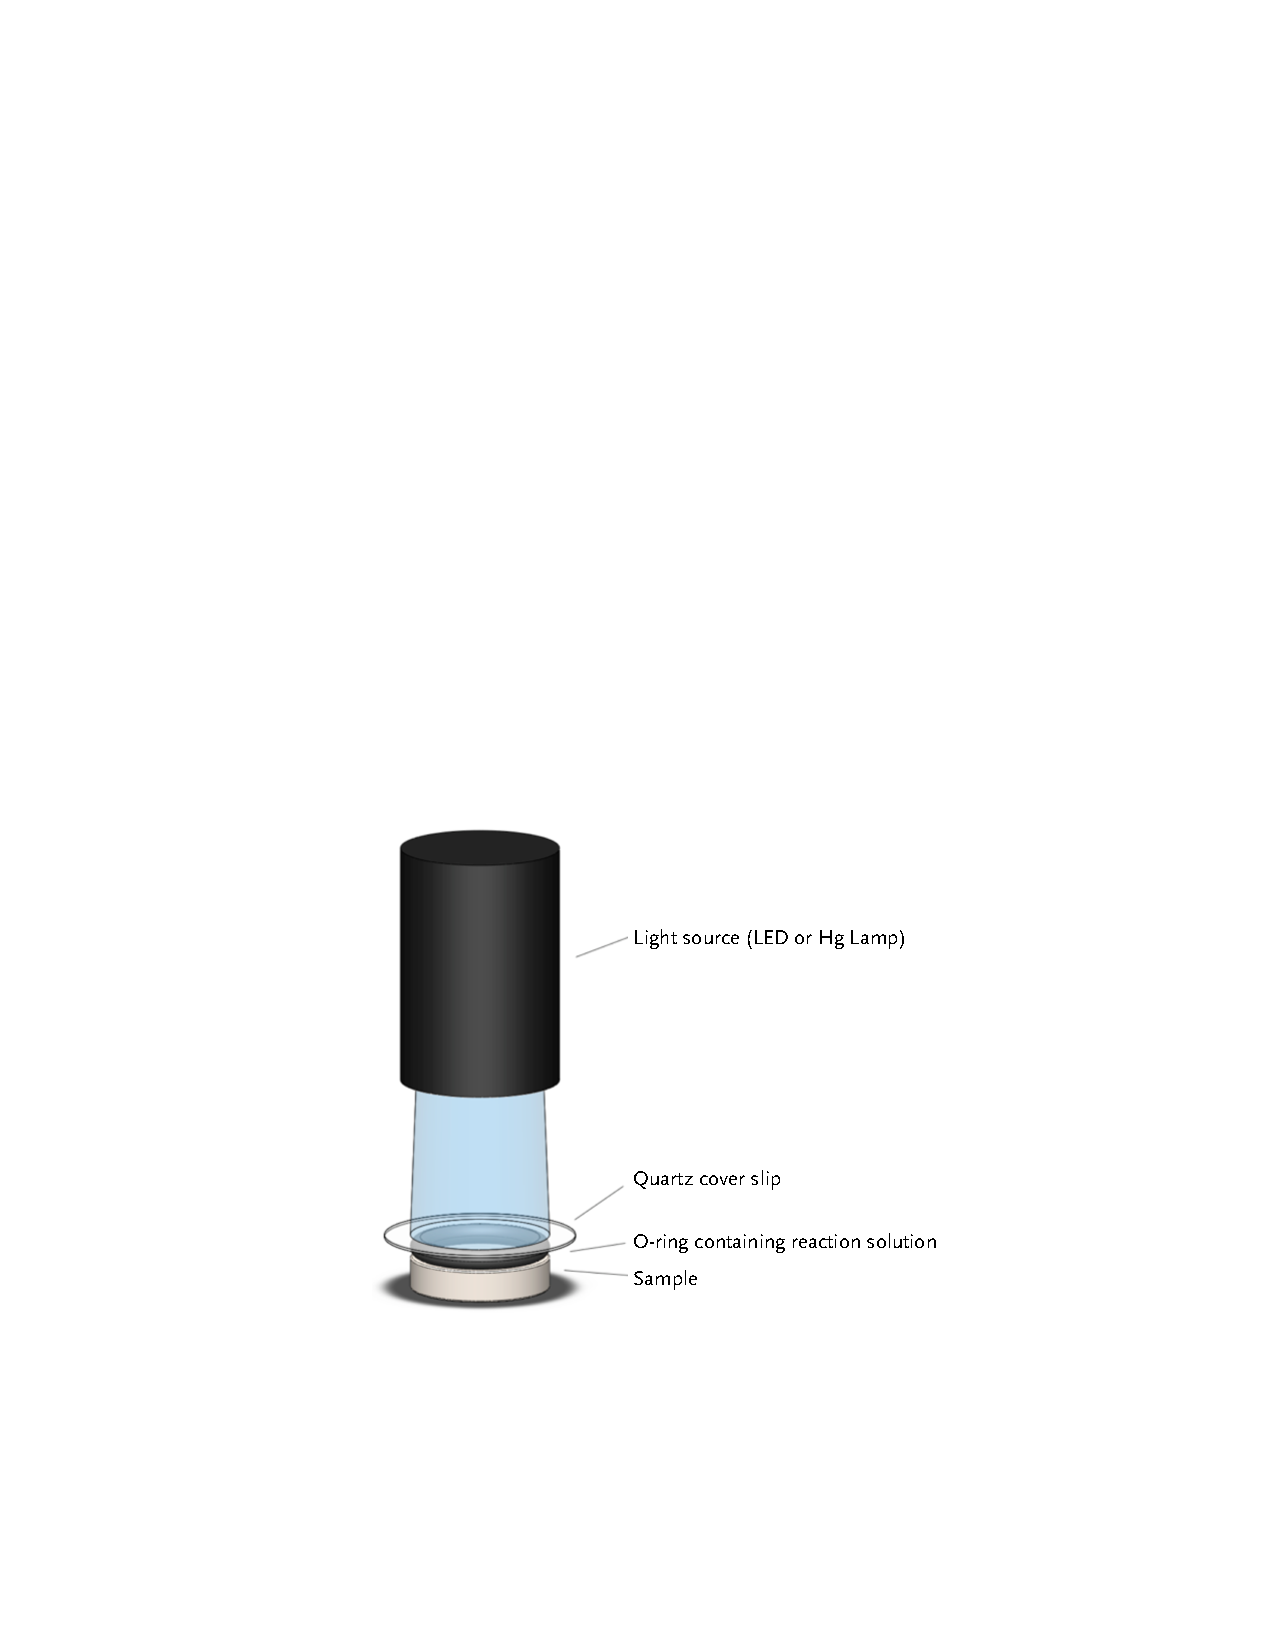
\includegraphics[width=0.8\textwidth]{rxnsetup.pdf}
\caption[Experimental setup for marker reactions]{%
	Experimental setup for performing photochemical marker 
	reactions. \ce{AgNO3} reaction solution is held in an 
	O-ring under a quartz cover slip and the light source 
	is positioned directly above the assembly.}
\label{fig:rxnsetup}
\end{center}
\end{figure}
%\sidefigure[Experimental setup for marker reactions]{%
%	Experimental setup for performing photochemical marker 
%	reactions. \ce{AgNO3} reaction solution is held in an 
%	O-ring under a quartz cover slip and the light source 
%	is positioned directly above the assembly.
%	\label{fig:rxnsetup}
%	}{%
%	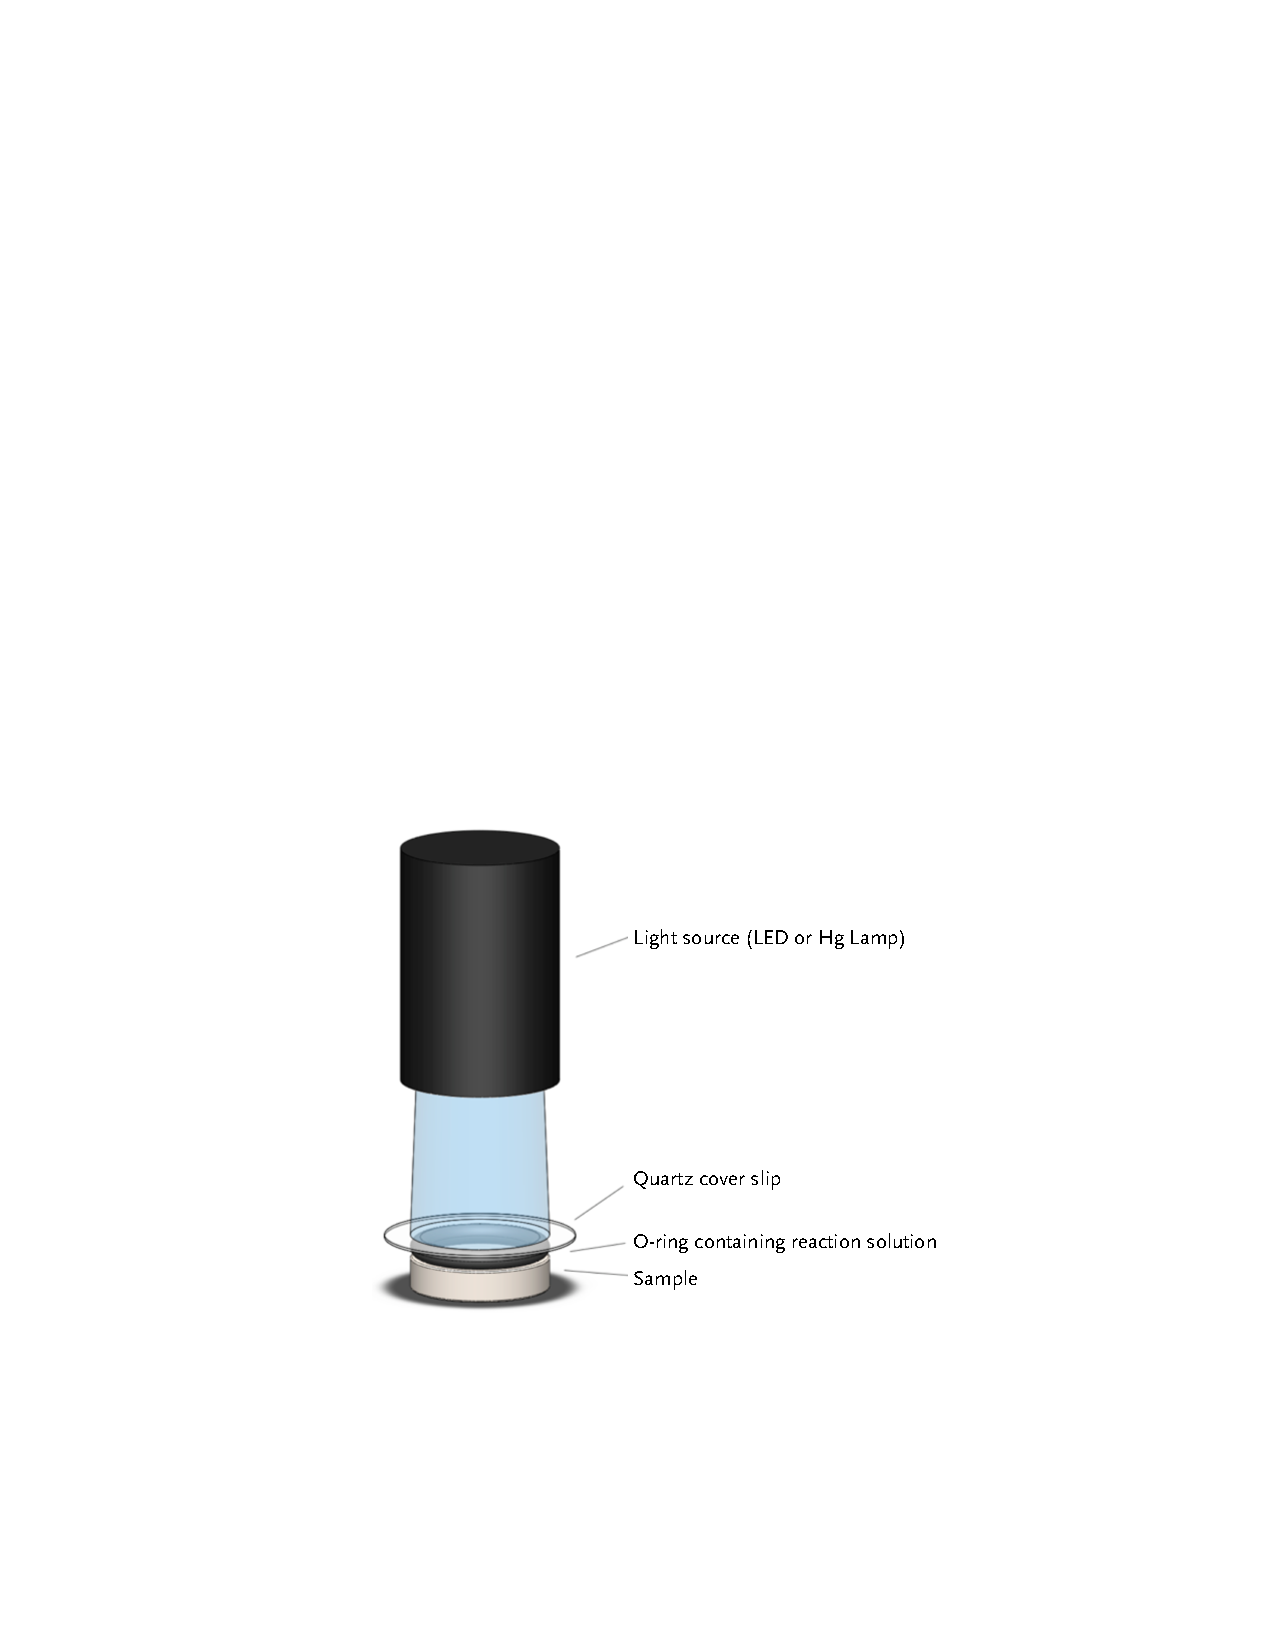
\includegraphics[width=\marginparwidth]{rxnsetup.pdf}
%}{0}
The established photochemical marker reaction of the reduction of silver ions in solution
to solid silver on the sample surface was used to study the photochemical reactivity of
the samples in this document.
\begin{equation}
\ce{Ag+ + e- -> Ag_{(s)}}
\end{equation}
This reaction deposits insoluble silver on the surface, marking the locations where
oxidation or reduction
occurred.\cite{Giocondi:2001gz,Burbure:2010go,Giocondi:2001bi,Burbure:2010ti,Bhardwaj:2010eh,%
Giocondi:2008ja,Lowekamp:1998ks,MorrisHotsenpiller:1998jq} The reaction product can
subsequently be observed using conventional atomic force microscopy methods.

For all marker reactions performed in this document, aqueous solutions of 0.115~\Molar
\ce{AgNO3} (Fisher Scientific, 99.96\%) were prepared. This specific concentration was
established by earlier
researchers,\cite{Giocondi:2001gz,Burbure:2010go,Giocondi:2001bi,Burbure:2010ti,Bhardwaj:2010eh,%
Giocondi:2008ja,Lowekamp:1998ks,MorrisHotsenpiller:1998jq} and results in an easily
observable reaction product on the surface after short illumination times.  Figure
\ref{fig:rxnsetup} schematically illustrates the setup for performing photochemical
reactions. A rubber O-ring was placed on the sample. A few drops of one of the solutions
were added into the O-ring. A quartz cover slip (\SI{0.2}{\milli\meter} thick) was placed
on top of the O-ring, held in place by surface tension. The cover slip creates a surface
perpendicular to the incident light, ensuring the same volume of solution and setup
geometry for all trials. The assembly was illuminated by commercially available blue
\abbr{LED} (\textlambda{}$_{\text{peak}}$ = \SI{470}{\nano\meter}, Philips Lumileds, San
Jose, CA) or \SI{300}{\watt} mercury arc lamp (Newport, Irvine, CA). The \abbr{LED} was
powered by a DC supply, set to deliver a constant current. Specific current and power
values for illumination are given along with corresponding experimental results in later
chapters. 

The duration of illumination varied, depending on the material and light source. The
reaction times used for collecting the data in this document were determined through
multiple trials, varying the reaction time in each trial. If the samples are allowed to
react for too long a duration, a the high amount of deposited solid makes characterization
difficult. Conversely, if the samples aren't reacted for a long enough time, the amount of
deposition is too low for observation. The times were selected because they resulted in an
observable and quantifiable amount of reaction product on the surface. Times for
individual photochemical experiments are listed in relevant sections of this document,
along with their corresponding results. After reaction, the samples were rinsed with
deionized water and dried with forced air.

To clean the surface of deposited products after reaction, the sample was wiped with a
cotton swab, then cleaned ultrasonically, first in methanol and then acetone. The acetone
was removed from the surface with a cotton swab. Subsequent microscopy demonstrates that
reaction products can be completely removed from the sample surface.

\label{masstransfer}
For all results presented in this document, it was assumed that mass transport of species
in the solution did not play a major role in interpreting the results from marker
reactions. The results from marker reactions presented in this document are all comparable
among experiments performed under the same conditions. For example,
\chapterref{single.crystal.reactivity} compares the relative reactivity of three
structures of \ce{Fe2O3} and \chapterref{fe2o3orientation} compares the relative
reactivity of different \ce{Fe2O3} grains on the same polycrystal. In these cases, certain
structures or grains were more reactive than others. It is possible that the rate of
reaction of the most reactive grains or structures was rapid enough that mass transfer
would be the limiting factor of reaction rate. However for each experiment, a comparison
between the most reactive and the least reactive structures could be made. Mass transfer
was not the limiting factor in the reactivity of the nonreactive or moderately reactive
cases, as under the same experimental conditions, other samples exhibited much higher
levels of reactivity.

\label{ph}
Reaction solution pH can potentially exert a significant effect on photochemical
properties of semiconductor photochemical systems. The pH of the solution affects the
nature of adsorbed species (typically, though not exclusively, \ce{H^{+}} and \ce{OH^{-}})
on the semiconductor surface, which in turn affect band bending within the space-charge
region of the semiconductor. The isoelectric point pH$_{\text{iep}}$ is defined as the pH
level at which the no net charge exists on the surface. A solution pH level higher than
this point causes a net negative charge on the surface, and a pH lower than the
pH$_{\text{iep}}$ causes a net positive charge on the surface. The effect of a solution pH
on the band edges of the semiconductor is given by
\begin{equation}
E_{CB}=E^{\degree}_{CB}+2.3kT\ln(\text{pH}-\text{pH}_{\text{iep}}),
\end{equation}
where $E{\degree}_{CB}$ is the band edge position at the isoelectric point. At room
temperature, this results in a band edge shift of \SI{60}{\milli\volt} with each
increasing pH unit. In the results presented in this document, pH effects are generally
not considered to have a major effect on the interpretation of activity results. The
reasoning for this is similar to that used for mass transfer effects.  In the case of
reactivity on \ce{Fe2O3} films, interpretations of results were comparative, with factors
affecting pH controlled across all experiments. As all films on single crystals were of
the same phase and orientation, negligible differences in pH effects between samples would
be expected. In the case of bulk \ce{Fe2O3} and \ce{Fe2O3} films on polycrystalline
substrates, in which the orientation of \ce{Fe2O3} is not controlled, differences in pH
could affect the reactivity of the individual film grains. The effect of surface
orientation on the isoelectric point varies depending on material. For example, the
isoelectric point of rutile \ce{TiO2} ranges between 3.2-3.7 for (100) faces and 5.5-5.8
for (001) faces,\cite{Bullard:2006jv} while the range of isoelectric points reported for
\textalpha-\ce{Fe2O3} is
6.3-8.5.\cite{Parks:1965ys,Kosmulski:2004vn,Kosmulski:2002kx,Kosmulski:2001ww} This
variance is somewhat significant, and can result in a band edge shift on the order of
\SI{100}{\milli\volt}. For the scope of the work presented in this document, that shift is
expected to be similar for all films, as preparation methods were consistent for all
samples, and reaction conditions were the same. 

\label{timescales}A last point to consider regarding the photochemical marker reactions
used in this work is differences in reactivity at various time scales. As the reaction
proceeds, the potential for changes in reaction conditions affecting reactivity exists.
The presence of silver on the surface immediately after the beginning of silver deposition
changes the overall band structure of the system. Early on in the reaction, most of the
surface is not covered by silver, but over longer timeframes, the affect of silver on the
band structure is no longer negligible. Once again, the comparative nature of the
interpretation of results should render negligible any affects from the change in the
electronic properties of the system from the deposition of silver. These effects would be
observed in all samples. Additionally, studies of the formation of silver nanoparticles in
aqueous solutions suggest that silver particles may grow
autocatalytically;\cite{Ershov:1993ci,VanHyning:2001vl} after the first silver atom forms,
additional silver atoms are easier to reduce and the rate of particle growth increases.
For the silver reaction product observed in the work presented in this document, distinct
silver particles are observed. Surfaces classified as more reactive in this work have more
individual particles on the surface. Thus the autocatalytic effects are not expected to be
responsible for the increased reactivity, as this would only expand already nucleated
particles.

\subsection{\abbr{EBSD}}
\label{subsec:exp.ebsd}


Electron backscatter diffraction (\abbr{EBSD}) was used as a primary tool for local
determination of film phase, orientation, and film|substrate orientation relationships.
Electron backscatter diffraction is a scanning electron microscopy technique that can
probe the local orientation and microstructure of a
material.\cite{Dingley:1997tw,Schwartz:2009ue} The technique relies on the interpretation
of an electron backscatter pattern. This pattern is generated when an electron beam
interacts with a flat surface, tilted at an angle of \texttildelow70\si{\degree}. The high
angle increases the intensity of backscattered electrons escaping from the sample.   As
backscattered electrons are generated in the electron beam interaction volume, they exit
the solid in patterns corresponding to the Bragg condition, a result of diffraction by
atomic planes within the material. The result is a  pattern of intersecting bands of high
intensity when the diffracted backscatter electrons reach a phosphor screen in the
\abbr{SEM} chamber. The phosphor screen is coupled to a \abbr{CCD} camera, which in turn
captures an image of the pattern. A schematic of this arrangement is depicted in Figure
\ref{fig:ebsdsetup}. 

\begin{figure}
\centering
	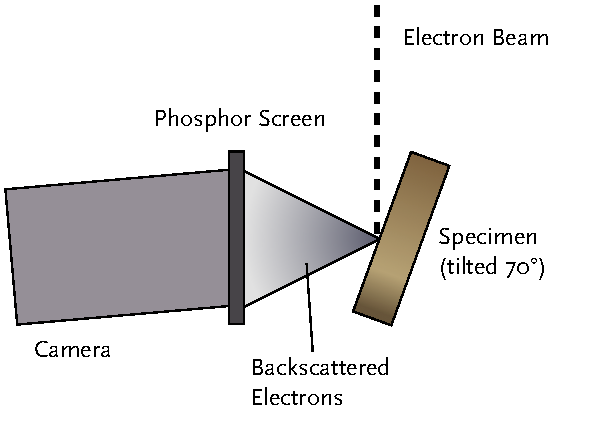
\includegraphics[width=0.8\textwidth]{ebsdsetup.pdf}
	\caption[Interior \abbr{SEM} arrangement for \abbr{EBSD} analysis]{%
	Schematic showing the interior arrangement of a scanning 
	electron microscope equipped with an \abbr{EBSD} detector.}
	\label{fig:ebsdsetup}
\end{figure}

\begin{figure}
\begin{center}
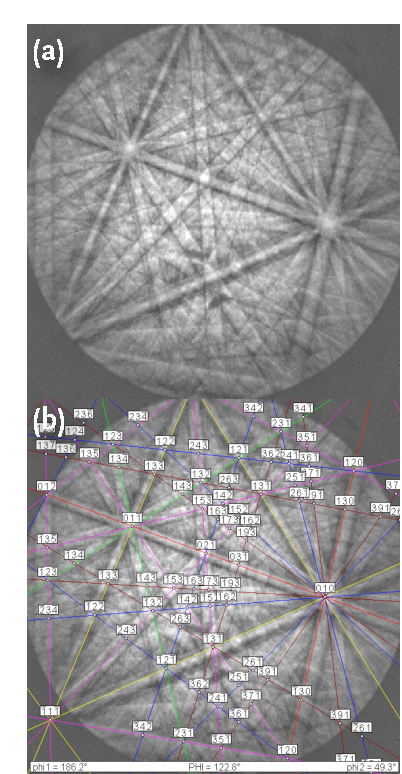
\includegraphics[width=0.4\textwidth]{ebsdsamples.pdf}
\caption[Electron backscatter diffraction patterns]{%
	Unindexed (a) and indexed (b) electron backscatter patterns 
	for a (111) oriented \ce{BiFeO3} grain.}
\label{fig:ebsdsamples}
\end{center}
\end{figure}
%\sidefigure[Electron backscatter diffraction patterns]{%
%	Unindexed (a) and indexed (b) electron backscatter patterns 
%	for a (111) oriented \ce{BiFeO3} grain.
%	\label{fig:ebsdsamples}
%	}{%
%	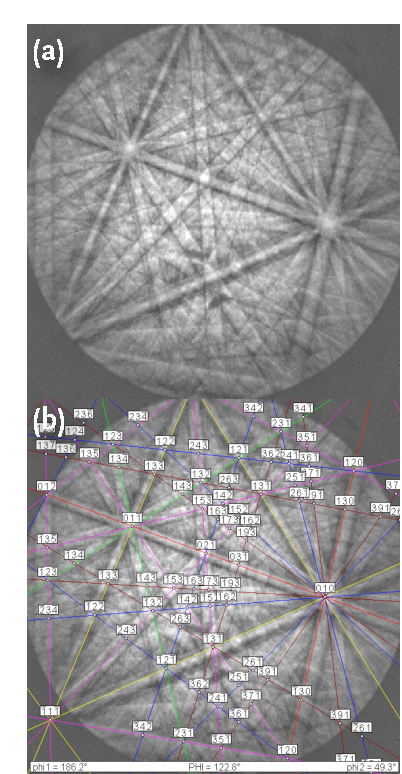
\includegraphics[width=\marginparwidth]{ebsdsamples.pdf}
%}{-21}
Computer software (\abbr{TSL}, \abbr{EDAX}, Mahwah, \abbr{NJ}), is used to then analyze
the location, intensity, and width of the bands. From this information, a set of Euler
angles is obtained that describes the orientation of the crystal. The Euler angles
represent the rotations that would rotate a crystal of a reference orientation to the
sample orientation. From the Euler angles, a set of Miller indices are generated
describing the local surface orientation in the crystal reference frame. A sample pattern
for a (111)-oriented \ce{BiFeO3} grain and the computer-generated band indexing is shown
in Figure \ref{fig:ebsdsamples}.


This procedure, if repeated across a raster pattern of points, can be used to map
orientations across a wide area of the sample. A computer can automate electron beam and
stage control, pattern acquisition, and pattern indexing. This technique has a benefit of
particular importance over other texture analysis techniques such as X-ray pole figures.
Orientation data is locally determined at each point, rather than over a wide area of the
sample simultaneously. This grants a great deal of flexibility when analyzing the
orientation data. Maps of grains, grain boundaries characterization, pole figures, and
inverse pole figures can be generated not just for the entirety  of the dataset, but also
for partitioned data of interest to a particular experiment. A representative map of grain
orientations for a \ce{SrTiO3} polycrystal is presented in Figure
\ref{fig:representativemap}.


\abbr{EBSD} was used in this work for analysis of \ce{Fe2O3} films grown on single crystal
and polycrystalline substrates. It was used for film phase identification, film
orientation measurement, and determination of epitaxial relationships between the film and
substrate. All electron backscatter experiments were performed in a Quanta 200
\abbr{FE-SEM} (\abbr{FEI} Company, Mahwah, \abbr{NJ}) equipped with and \abbr{EBSD}
detector using TSL software (\abbr{EDAX}) for pattern acquisition and data analysis.
\begin{figure}
\begin{center}
\includegraphics[width=0.75\textwidth]{representativemap.png}
\caption[Representative \abbr{EBSD} inverse pole map]{%
	Representative \abbr{EBSD} inverse pole map. This map depicts the 
	microstructure of a \ce{SrTiO3} polycrystal.}
\label{fig:representativemap}
\end{center}
\end{figure}
%\sidefigure[Representative \abbr{EBSD} inverse pole map]{%
%	Representative \abbr{EBSD} inverse pole map. This map depicts the 
%	microstructure of a \ce{SrTiO3} polycrystal.
%	\label{fig:representativemap}
%	}{%
%	\includegraphics[width=\marginparwidth]{representativemap.png}
%}{0}
All experiments were performed in a low-vacuum atmosphere in the presence of water vapor.
This allows for analysis of weakly conducting samples such as those used in this
experiment without the complications of sample charging from the electron beam. In all
cases, clearly indexable electron backscatter diffraction patterns were obtained, even
under low-vacuum conditions. The working distance was \SI{15}{\milli\meter}. The tilt
angle was always within \SI{0.1}{\degree} of of \SI{70}{\degree} from horizontal.
Accelerating voltage was 20.0-25.0~\si{\kilo\volt}. Exposure parameters for the \abbr{CCD}
camera were adjusted as needed for each scan. Generally, the exposure time was adjusted to
achieve a frame rate of 50-100~frames~per~second. Other parameters were then adjusted to
obtain diffraction patterns with good contrast and accurate indexing of diffraction bands,
as determined by manual inspection and computer-generated confidence index (\abbr{CI}). 
Computer image processing was used to improve the pattern quality. An average background
signal was collected while scanning the beam over the sample. This background is
subtracted by the computer for all collected patterns, to increase the contrast of the
pattern. In some cases, additional processing such as dynamic background subtraction and
normalizing of the intensity histogram were required to obtain good patterns. Scan
parameters such as the scan area and distance between points were changed from sample to
sample, and were dependent upon grain size, frame rate, and available microscope time.


\subsection{X-ray}
\label{subsec:exp.xray}


Conventional X-ray diffraction (\abbr{XRD}) characterization was used to verify the phase
of polycrystalline samples and to determine the phase and orientation of thin film
samples. In the experiments presented in this document, X-ray diffraction was used to
verify the presence of a desired phase in synthesized materials. X-ray scans were
performed using a Panalytical X'Pert Pro \abbr{MPD} diffractometer (Panalytical,
Westborough, \abbr{MA}). After the diffraction pattern was collected, the results were
compared with tabulated diffraction data from the International Center for Diffraction
Data database. 

X-ray reflectometry\cite{birkholz2006thin} was used to measure film thickness and
calibrate growth rate. X-ray reflectivity relies upon interference between reflected beams
from layers of material with different density. In this technique, the incident angle of
the X-ray beam is slowly varied. As the reflected angle is changed, interaction between
the reflected beam switches between constructive and destructive interference, causing
fringes in the collected intensity data. Software is then used to calculate film
thickness, given information about the composition and density of the materials under
investigation. X-ray reflectometry scans were carried out on a Panalytical diffractometer.
Using this data, the growth rate for films under the deposition conditions used in this
document was determined. This growth rate was then used to select the appropriate
deposition duration to deposit films of desired thicknesses. 


\subsection{Scanning Probe Microscopy}
\label{subsec:exp.scanningprobe}


Sample surface profiles before and after photochemical reaction were examined using
contact mode atomic force microscopy (\abbr{AFM}). \abbr{AFM} determines nanoscale
displacements by measuring the deflection of a laser beam reflected off a microscopic
cantilever.\cite{Murphy:1987wc} Attached to the cantilever is a tip that moves along the
surface of the sample. Piezoelectric elements are used to scan the tip across the sample.
As the height of the sample changes, the tip is deflected, changing the measured intensity
of the reflected beam. The microscope adjusts the height of the tip to account for the
deflection, recording the magnitude of the adjustment. The records for the entire scanned
area are constructed into an image corresponding to the topography of the sample. 

\abbr{AFM} micrographs of sample surfaces were recorded before and after photochemical
marker reactions. Conventional contact and semicontact methods were
used.\cite{Anonymous:YBI-TQ6H} All scans were collected on either an \abbr{NT}egra or
Solver Next \abbr{AFM} (\abbr{NT-MDT}, Moscow, Russia). For contact mode images, aluminum
coated silicon tips with a force constant of 0.11~\si{\newton\per\meter} were used
(\abbr{CSG10, NT-MDT}). For semicontact images, aluminum coated silicon tips with a rated
resonant frequency of 240~\si{\hertz} were used (\abbr{NSG10, NT-MDT}). Scan rates were
chosen based on the size of the scan area, and were in the range of 0.5-2~\si{\hertz}.  

The local surface polarization of \ce{BiFeO3} was examined using piezoresponse force
microscopy (\abbr{PFM}). Piezoresponse force is a contact mode technique used to determine
the local polarization direction of ferroelectric
materials.\cite{Kalinin:2002hq,Kalinin:2006bg,Jungk:2006he,Rodriguez:2004bu} While
scanning the surface in contact mode, an \abbr{AC} bias is applied to the tip. Because
ferroelectric materials are also piezoelectric, the applied bias causes a local expansion
or contraction of the material. A lock-in amplifier is used to measure the phase of the
expansion and contraction. From this data, the out of plane direction of polarization of
the surface is determined. \abbr{PFM} measurements were collected using a
Solver\abbr{NEXT} \abbr{AFM}. Titanium nitride coated tips with a force constant of
11.8~\si{\newton\per\meter} were used (\abbr{NSG10}/Au, \abbr{NT-MDT}).

	\part{Experiments on Photochemical Activity}
		% !TEX root = base.tex 

\chapter{Orientation Dependent Hematite Reactivity}
\label{ch:fe2o3orientation}


\chintro{Bulk and surface orientation have been shown to affect the photochemical
reactivity of semiconductor surfaces. Orientation dependent photochemical reactivity has
been observed for oxide semiconductors. For example, rutile and anatase \ce{TiO2}
microcrystals,\cite{Ohno:2002fn} thin film rutile \ce{TiO2},\cite{Anonymous:YQSV8dnc} and
polycrystalline rutile \ce{TiO2}\cite{Lowekamp:1998ks} have been shown to exhibit
anisotropic activity. Microcrystals of \ce{BaTiO3},\cite{Giocondi:2008ja}
\ce{SrTiO3},\cite{Giocondi:2007fa} and \ce{Sr2Nb2O7}\cite{Giocondi:2008ja} also exhibit
different levels of reactivity for different crystal faces, as does bulk \ce{SrTiO3}
single crystals\cite{Giocondi:2003wc} and polycrystals.\cite{Giocondi:2003wn} Existing
literature on the anisotropic photochemical activity of hematite differentiates between
the basal and prismatic faces of hematite crystals.\cite{Eggleston:2009ic} There are no
reports that differentiate the properties of various prismatic faces and high index
orientations. The results presented in this chapter further our understanding of the
anisotropic photochemical properties of \ce{Fe2O3}, including high index orientations.
In order to accurately decouple effects reported in subsequent chapters from
microstructure, substrate charge, and film orientation on photochemical activity, the
dependence of photochemical activity on crystallite orientation was examined.  These
results provide the baseline information for interpretation of other photochemical
experiments on \ce{Fe2O3} presented in this document.}



\section{Experimental Details}
\label{sec:ch9experimental}


Electron backscatter diffraction (\abbr{EBSD}) was used to determine grain orientations of
a polycrystalline \textalpha-\ce{Fe2O3} pellet. By using a polycrystalline sample, a wide
variety of orientations, covering the entire range of the standard stereographic triangle
representing all possible surface orientations, can be examined in a single experimental
run. 

A polished \ce{Fe2O3} pellet was prepared as described in Chapter~\ref{ch:experimental}.
To promote grain growth, the pellet was sintered for at \SI{1200}{\degreeCelsius} for
\SI{48}{\hour} in air, rather than the sintering procedure in Chapter
\ref{ch:experimental}. No other changes from the established sample synthesis procedure
were made. An orientation map of the sample was obtained using electron backscatter
diffraction. Backscatter patterns were of consistent high quality over the entire examined
area. Acquisition was performed under high vacuum with an accelerating voltage of
\SI{20}{\kilo\volt}. 

Photochemical activity was measured using the established reaction of the reduction of
aqueous silver ions to neutral solid silver. Reactions were carried out under illumination
from a narrow spectrum blue \abbr{LED} (Philips Lumiled, \textlambda$_\text{peak}$ =
\SI{470}{\nano\meter} and broad spectrum Xe arc lamp (\SI{150}{\watt}, Newport, Bozeman,
\abbr{MT}). The reaction time was varied depending on the light source and characterization
technique. Table \ref{tab:reactiontimes} lists the reaction times used for this work.
\begin{table}
\begin{center}
  \begin{tabular}{lrr}

   Characterization Method & Xe Lamp  & Blue \abbr{LED}  \\
  
   \cmidrule(lr){1-1}
   \cmidrule(lr){2-2}
   \cmidrule(lr){3-3}
   
   Optical & \SI{5}{\minute} & \SI{15}{\minute} \\
   \abbr{SEM} & \SI{5}{\minute} &  --\\
   \abbr{AFM} & \SI{30}{\second} & -- \\

\end{tabular}
\end{center}
  \caption[Reaction times for photochemical experiments]{Reaction times for photochemical
experiments presented in this chapter. Reaction time varied depending on illumination
source and observational technique. These times were selected to provide optimal imaging
conditions for each technique.}
  \label{tab:reactiontimes}
\end{table}
Reaction times were chosen to provide the best level of reaction product for the
respective observation technique. For example, for optical microscopy, a large amount of
reaction product will provide maximum contrast, but for atomic force microscopy, too many
solid silver particles on the surface will cause difficulty in accurately measuring the
topography of the surface. 

The surface of the sample was examined before and after photochemical reaction with
scanning electron (\abbr{SEM}), atomic force (\abbr{AFM}), and Kelvin probe force
(\abbr{KFM}) microscopy. Scanning electron microscopy allow for rapid analysis of many
grains simultaneously, but grains that have low (but nonzero) levels of reactivity may be
missed. Atomic force measurements provide extremely accurate measures of reactivity,
including low and moderate levels of reaction product, but are comparatively time
consuming and difficult to obtain. All methods were used to verify the presence of
reaction product on a wide range of crystallite orientations. Kelvin probe force
microscopy was used to examine the local surface potential of reactive and nonreactive
grains.

Scanning electron microscopy was performed using a Quanta 200 \abbr{FE-SEM} 
(\abbr{FEI} Company, Mahwah,
\abbr{NJ}) with an accelerating voltage of \SI{5.0}{\kilo\volt}. \abbr{AFM} images were
collected using an \abbr{NT}egra \abbr{AFM} (\abbr{NT-MDT}, Moscow) using standard
semicontact techniques. \abbr{KFM} images were obtained using a Solver\abbr{NEXT}
\abbr{AFM} (\abbr{NT-MDT}).


\section{Results}
\label{sec:ch9results}


\subsection{Scanning Electron Microscopy}
\label{subsec:ch9sem}


\figureref{semimages} shows \abbr{SEM} micrographs of the \ce{Fe2O3} surface after
reaction.
\begin{figure}
	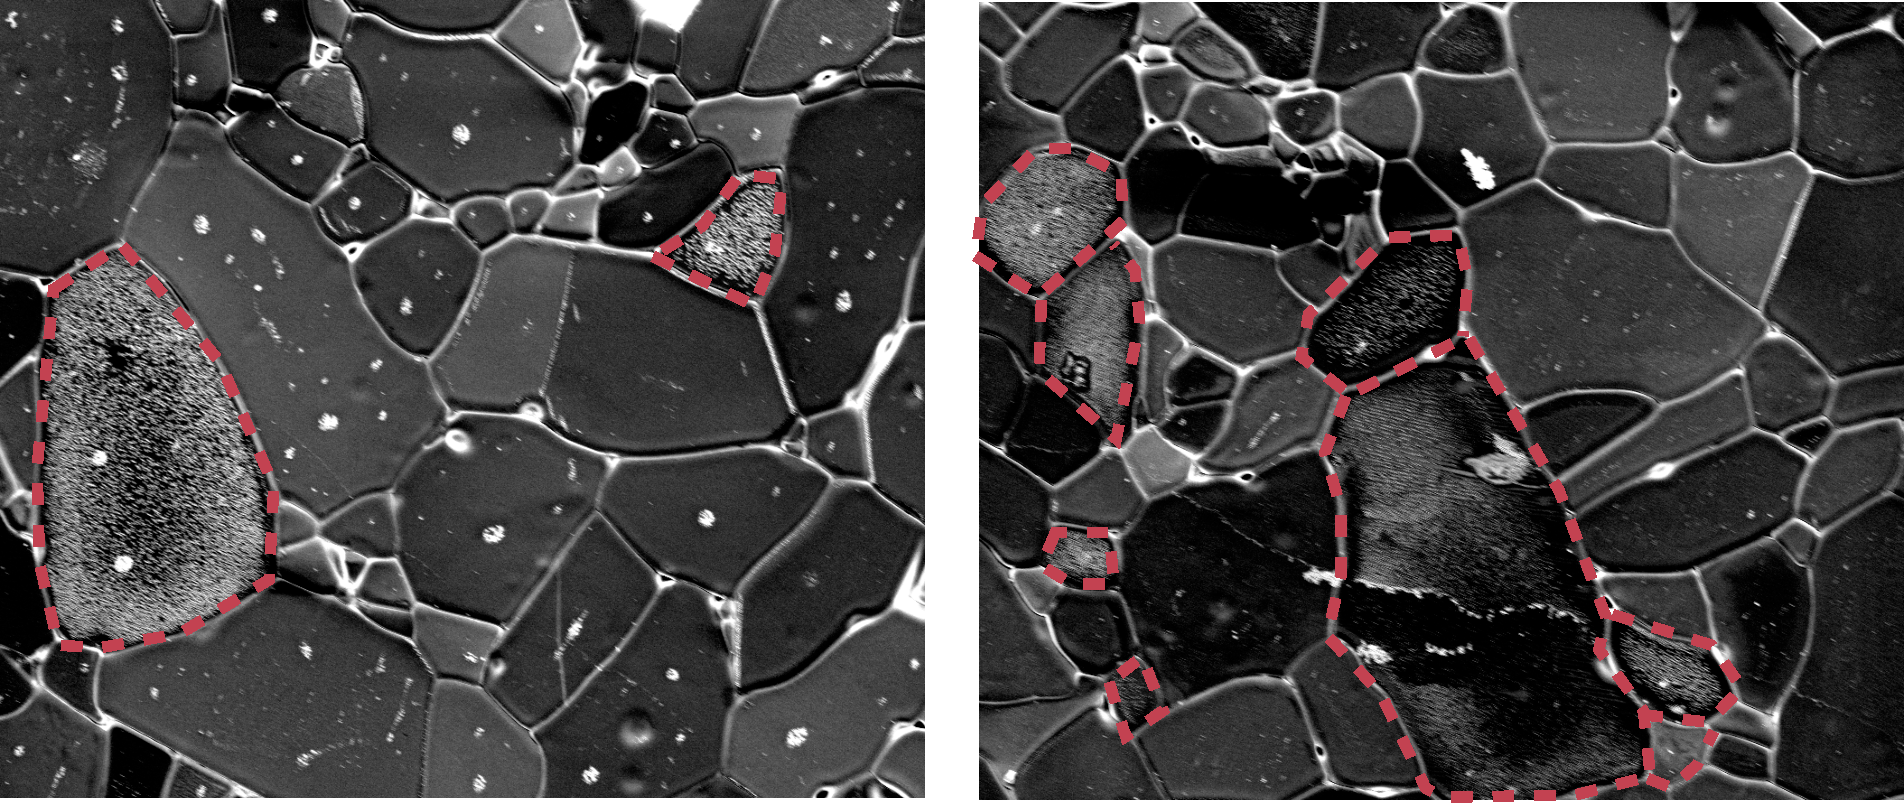
\includegraphics[width=\textwidth]{semimages.pdf}
	\caption[Representative \abbr{SEM} micrographs after photochemical reaction]{%
		Representative \abbr{SEM} micrographs of \ce{Fe2O3} polycrystals taken after
photochemical reaction showing reactive and nonreactive grains. Grains were identified as 
		reactive by manual inspection. Reaction product appears as bright white areas
within a grain. Reactive 
		grains are outlined in red in these micrographs. Other sources of white contrast
include grain boundaries and 
		pores.}
	\label{fig:semimages}
\end{figure}
Reaction product appears as bright areas within grains in the \abbr{SEM} micrographs.
Additional white contrast appears in the form of grain boundaries and pores, presumably
arising from charging of the weakly conducting sample. Reactive grains are outlined on the
micrographs in \figureref{semimages}. Grains were manually identified as reactive or
nonreactive. \abbr{SEM} images were collected to cover a large area of the sample. The
images in \figureref{semimages} are representative of all collected micrographs.

\figureref{ebsdmapsem} shows the complete inverse pole map collected via \abbr{EBSD} and a
subset of the map corresponding to the grains marked as reactive during \abbr{SEM}
observation.
\begin{figure}
	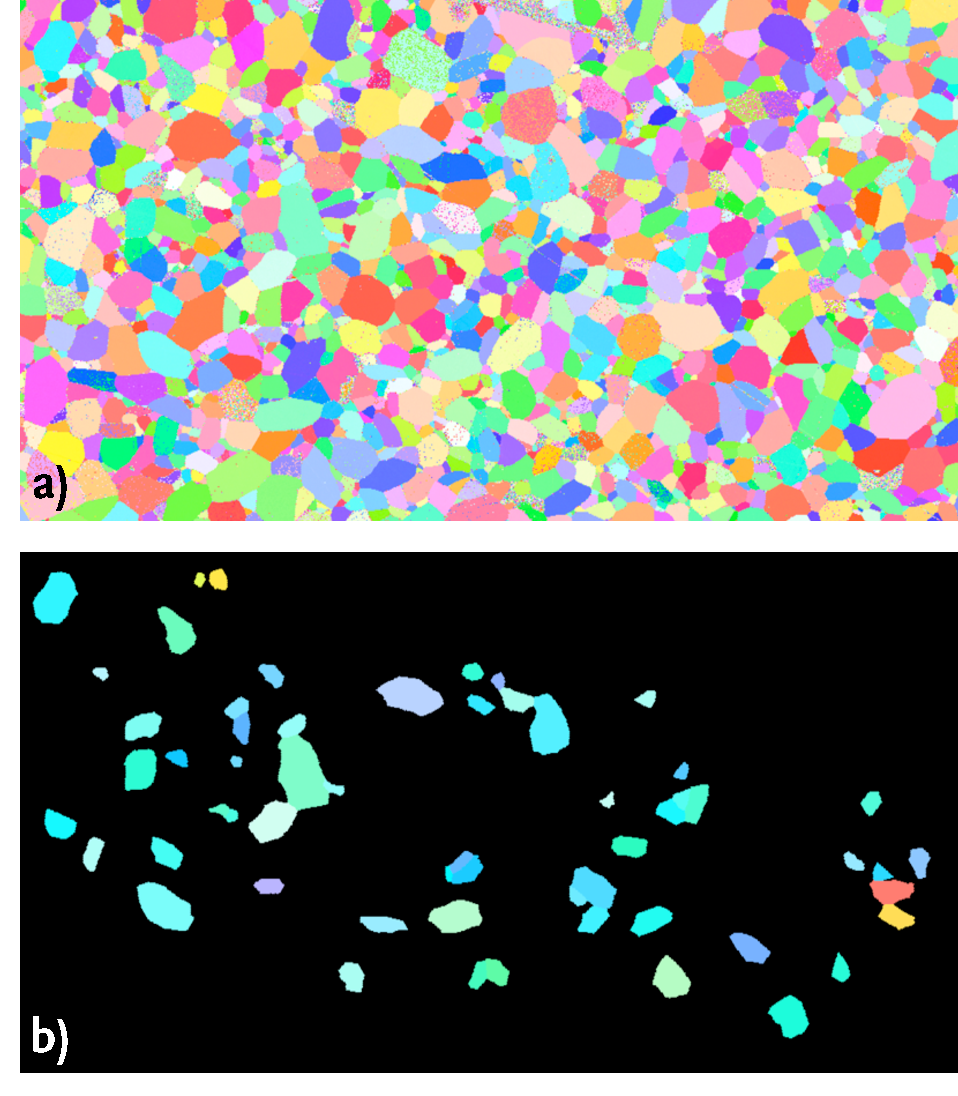
\includegraphics[width=\textwidth]{ebsdmapssem.pdf} %maybe make these side by side and
%then have a wholewidth figure
	\caption[Inverse pole maps of \ce{Fe2O3} surface]{%
		Electron backscatter diffraction inverse pole maps of the 
		observed area of the \ce{Fe2O3} surface. (a) Map including 
		all grains in the observed area. (b) The subset of grains 
		identified as reactive during \abbr{SEM} analysis of the surface 
		after photochemical reaction with \ce{AgNO3}. These grains 
		correspond to the points on the standard stereographic triangle 
		in \figureref{semtriangle}. The similar color of these 
		grains in the inverse pole map suggests that the majority 
		of active grains are similarly oriented. }
\label{fig:ebsdmapsem}
\end{figure}
\begin{figure}
	\centerline{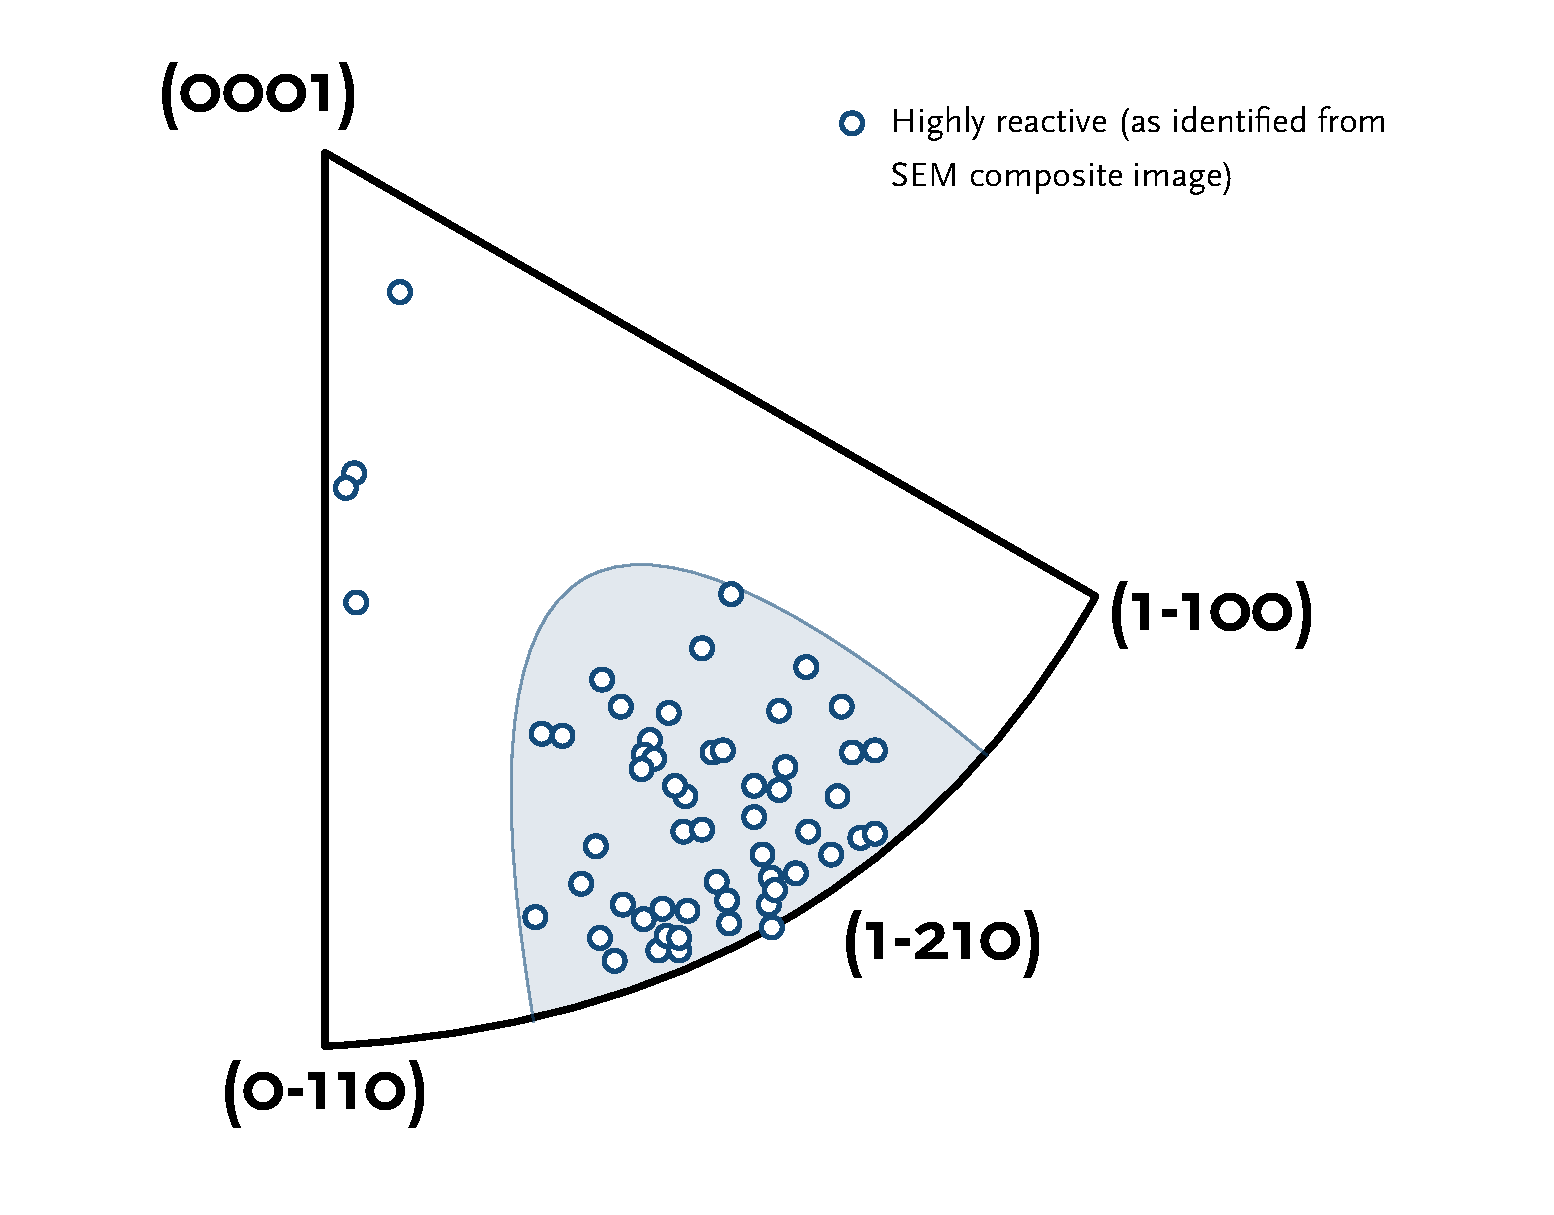
\includegraphics[width=0.6\textwidth]{semtriangle.pdf}}
		\caption[Reactive grains from \figureref{ebsdmapsem}]{%
			Reactive grains from \figureref{ebsdmapsem} plotted on 
			the standard stereographic triangle for hexagonal crystals. Each 
			point in the triangle represents the orientation of a grain 
			identified as reactive. The blue shaded area outlines the cluster 
			of highly reactive grains near the (1\={2}10) orientation. With 
			four exceptions, all observed reactive grains were oriented near 
			this orientation.}
	\label{fig:semtriangle}
\end{figure}
The grains identified as reactive generally fall within a similar color range, suggesting
strong orientation effects on photochemical activity. The difference between reactive and
nonreactive grains was very obvious for most grains; reactive grains were generally
completely or mostly covered with bright reaction product, while nonreactive grains were
completely devoid of any contrast from solid silver on the surface. The points identified
as reactive were plotted on the standard stereographic triangle for hexagonal crystal
systems, presented in \figureref{semtriangle}. This triangle represents the entire
possible set of orientations. Points on the triangle represent observed reactive grains.
With four exceptions, all points lie within about 10-15\degree{} from the (1\={2}10) pole.


\subsection{Atomic Force Microscopy}
\label{subsec:ch9afm}


To verify the rapid but imprecise classifications of reactivity obtained via
scanning electron microscopy, the reacted sample was examined using atomic force
microscopy. The results from the \abbr{SEM} images were used to determine appropriate
locations for study. To increase the amount of data obtained through \abbr{AFM}, scan
locations were selected that contained multiple grains, including both reactive and
nonreactive grains as identified in \abbr{SEM} images. Six scan areas were selected,
comprising a total of approximately 60 grains of varying orientation.
\figureref{fe2o3afmmap} shows an inverse pole map displaying which grains were observed
using \abbr{AFM}.
\begin{figure}
	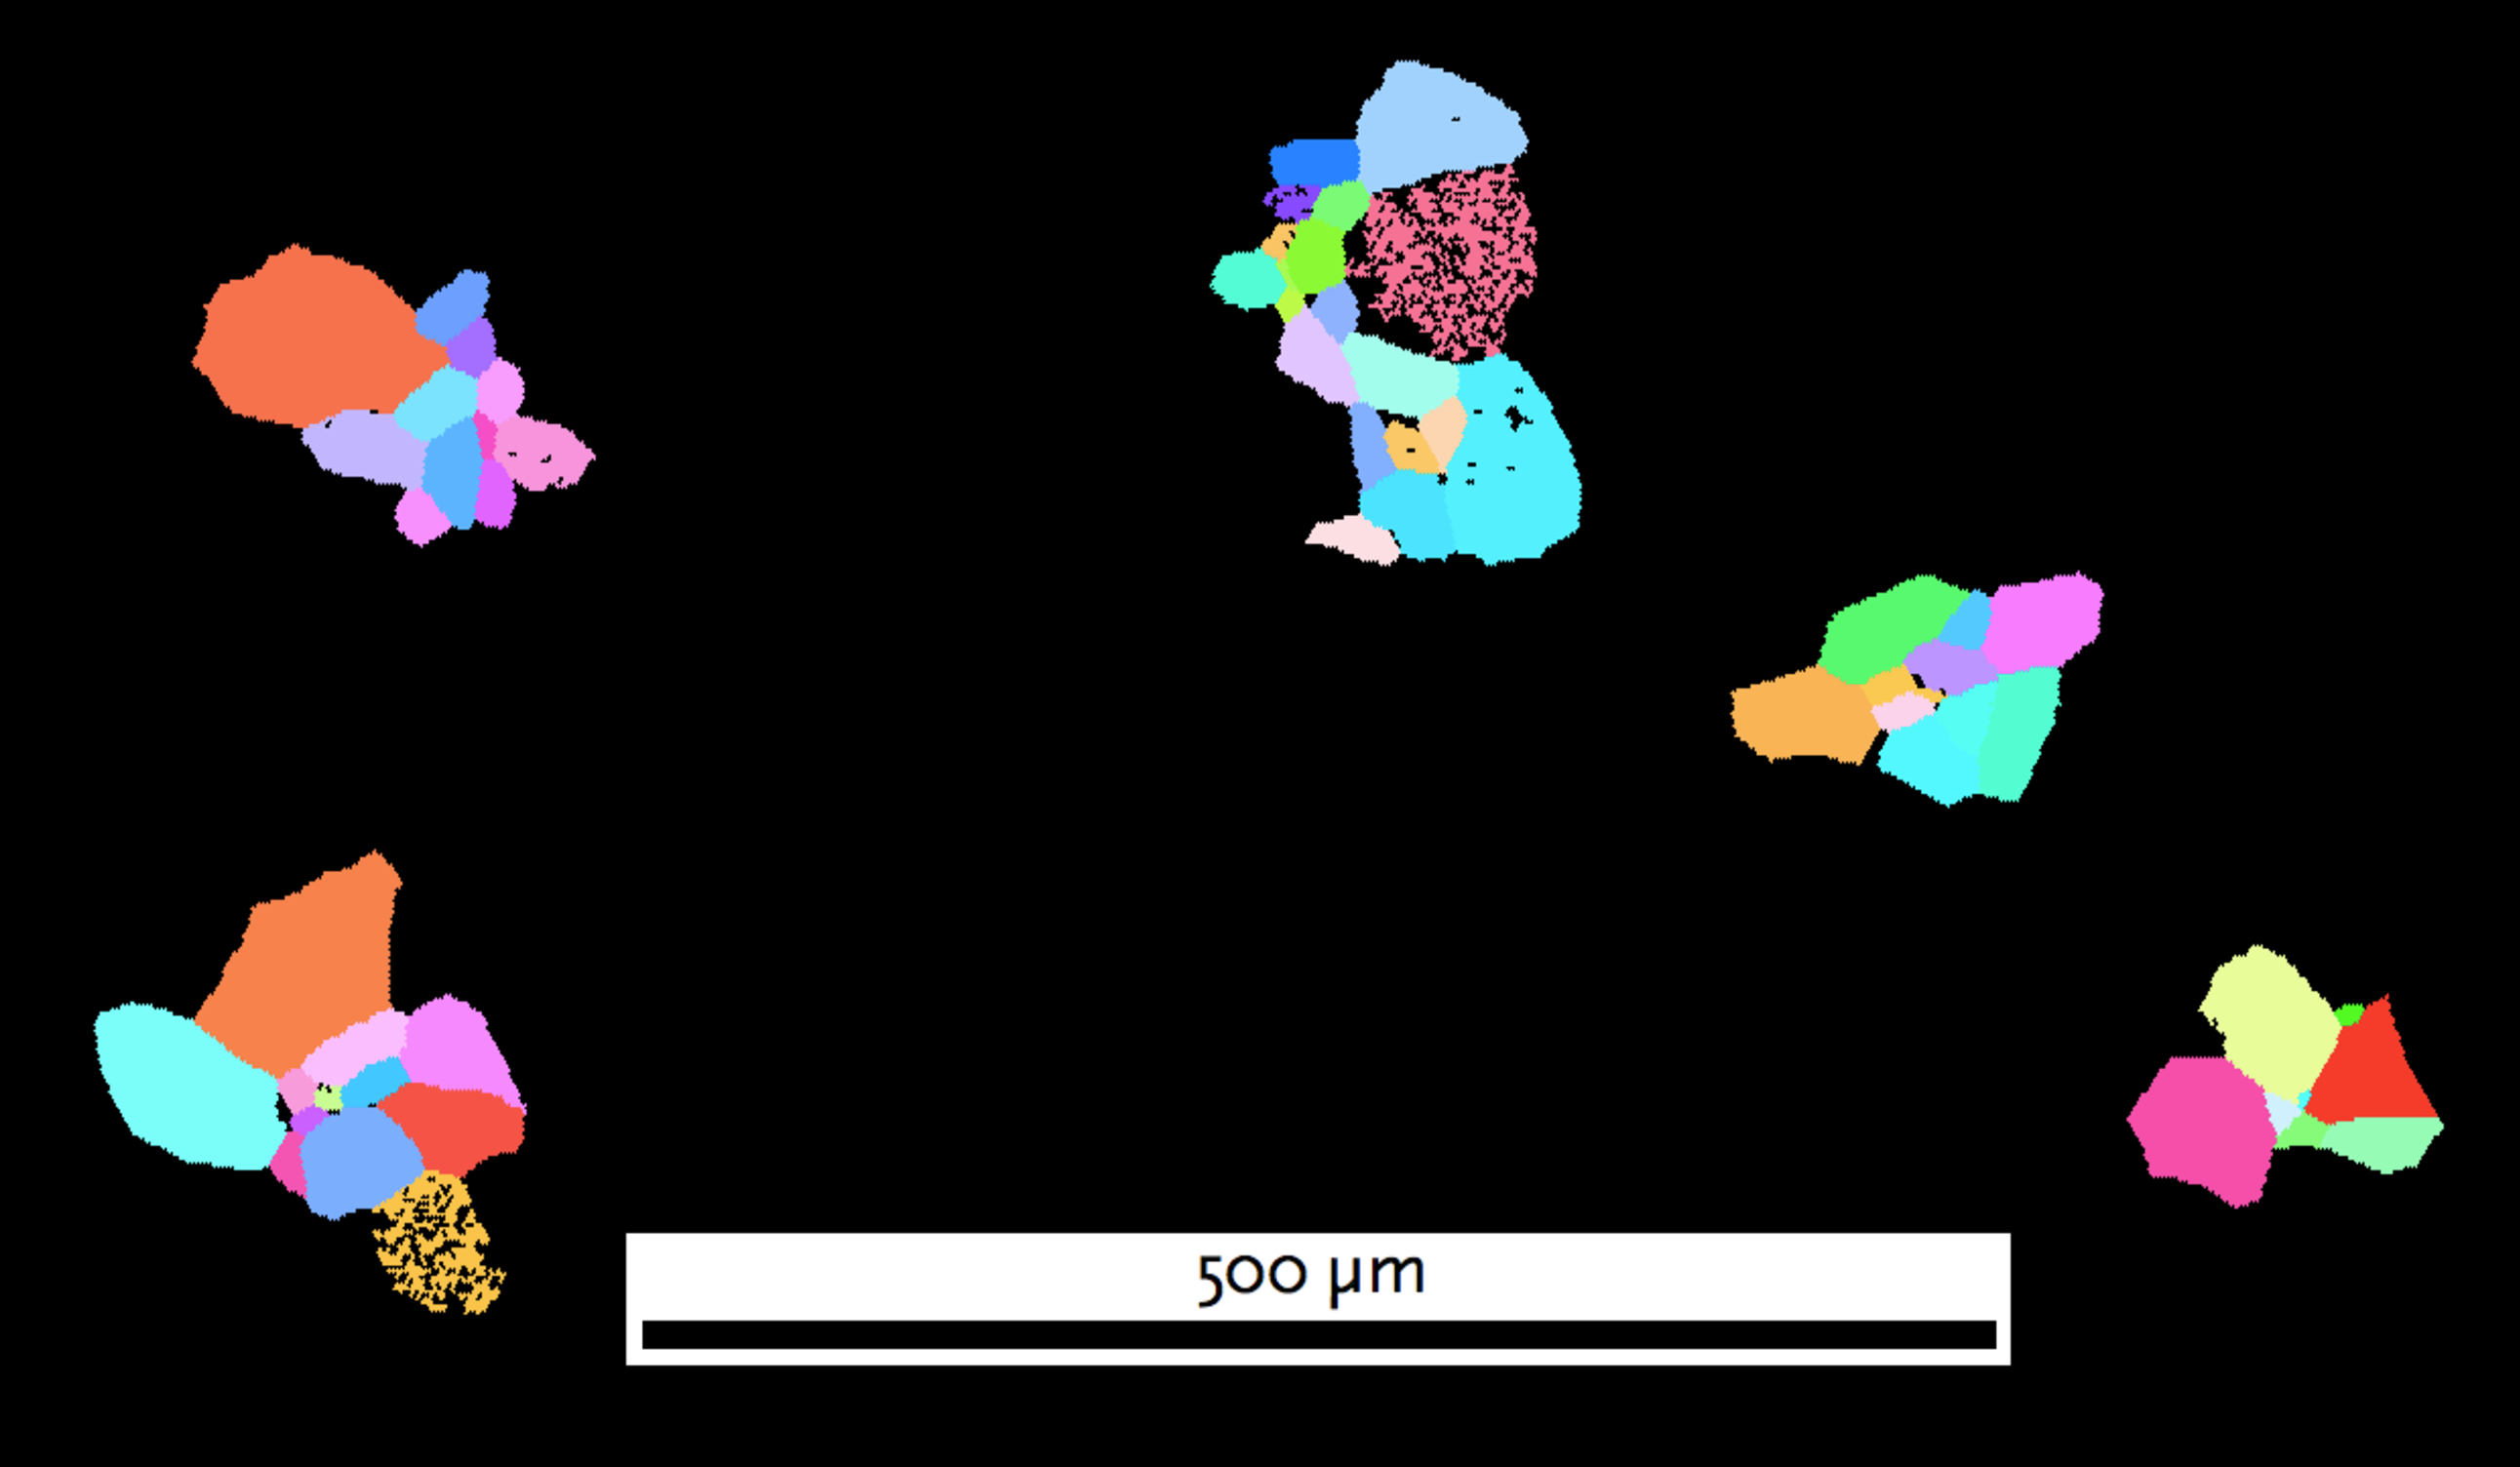
\includegraphics[width=\textwidth]{fe2o3afmmap.pdf}
	\caption[Inverse pole map of grains observed using \abbr{AFM}.]{%
		Inverse pole map showing the portion of grains observed using atomic force
microscopy. This source data for this 
		figure is the same as for \figureref{ebsdmapsem}.}
	\label{fig:fe2o3afmmap}
\end{figure}

Figures \ref{fig:fe2o3afmscans}(a)-(c) show the representative \abbr{AFM} scans of the
sample surface after reaction under illumination from a Xe arc lamp for \SI{30}{\second}.
All scans have dimensions of \SI{50}{\micro\meter} \texttimes{} \SI{50}{\micro\meter}.
Three levels of reactivity were manually assigned to each grain. Grains that were entirely
covered in reaction product were labelled highly reactive. In \figureref{fe2o3afmscans},
these grains are outlined in blue. Grains with partial reactivity, such as reactive areas
or grain edges were labeled moderately reactive. \figureref{fe2o3afmscans}(c) contains a
moderately reactive grain, outlined in green.
\begin{figure}[b]
	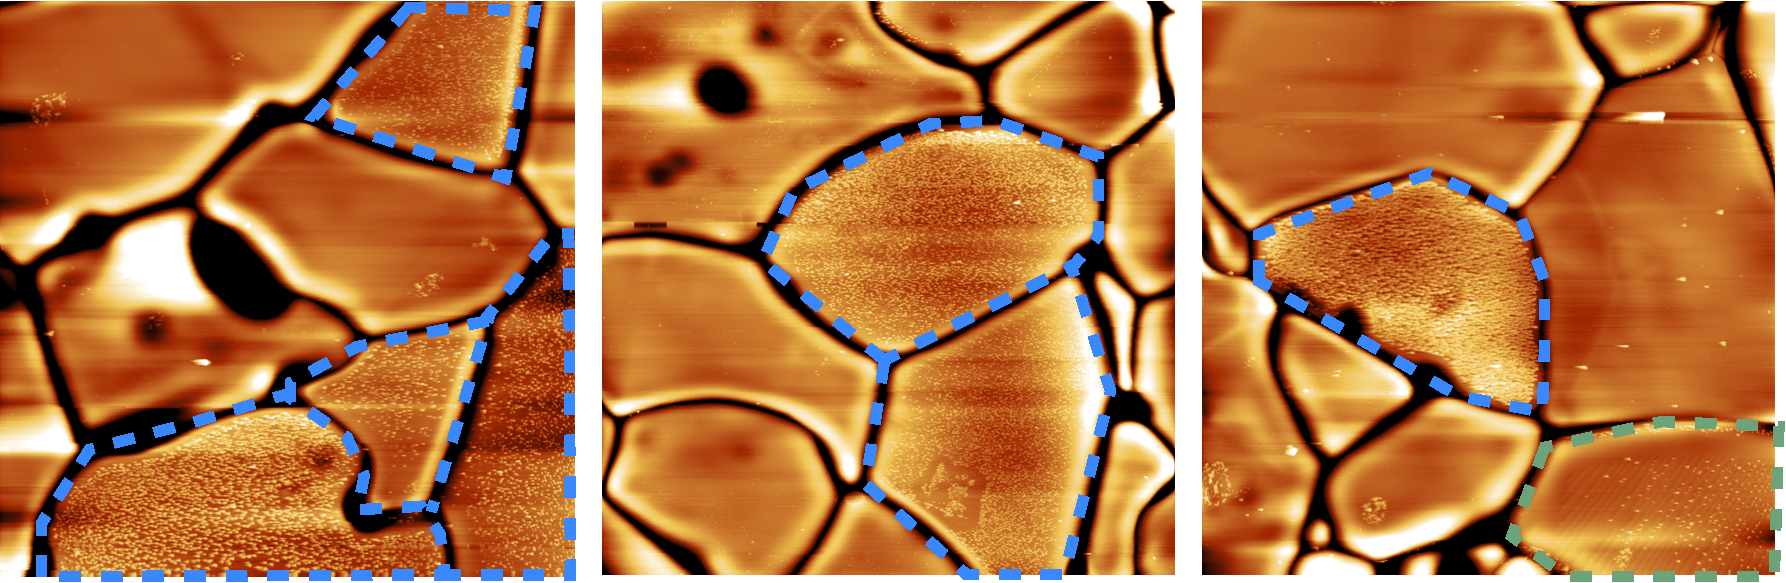
\includegraphics[width=\textwidth]{fe2o3afmscans.pdf}
	\caption[Representative \abbr{AFM} scans of three examined areas]{%
		Representative \abbr{AFM} scans of three examined areas. Highly reactive grains
are outline in blue. 
		Moderately reactive grains are outlined in green. These scans are representative
of all scans 
		obtained via \abbr{AFM}. The size of each image is \SI{50}{\micro\meter}
\texttimes{} \SI{50}{\micro\meter}.}
	\label{fig:fe2o3afmscans}
\end{figure} 

\begin{figure}
	\centerline{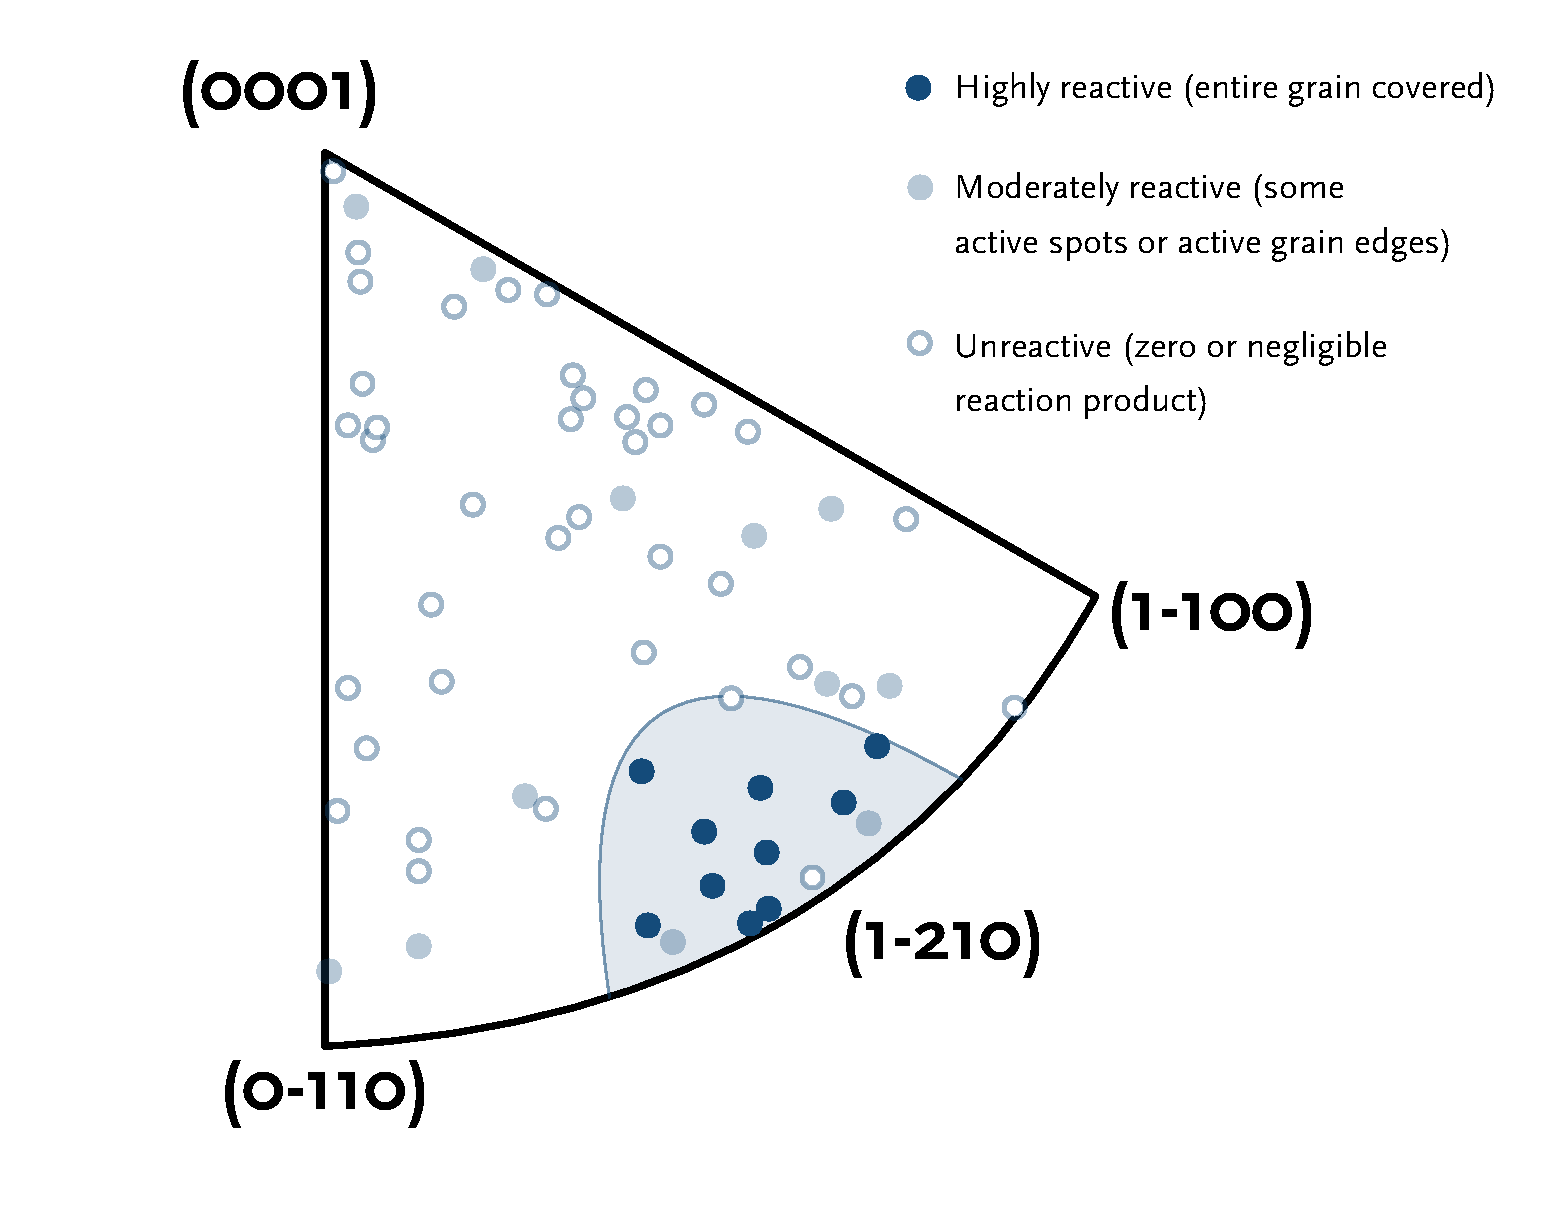
\includegraphics[width=0.6\textwidth]{afmtriangle.pdf}}
		\caption[Reactive grains from \figureref{fe2o3afmmap}]{%
			All grains from \figureref{fe2o3afmscans} plotted on the 
			hexagonal standard sterographic triangle. Highly reactive grains 
			are dark blue, moderately reactive grains are light blue, and 
			nonreactive grains are open circles. All highly reactive grains 
			are located near the (1\={2}10) orientation.}
	\label{fig:afmtriangle}	
\end{figure}
After classifying all grains contained in the full set of \abbr{AFM} scans, each point was
plotted on the standard stereographic triangle for hexagonal crystal systems, similar to
\figureref{semtriangle}. The resulting triangle for \abbr{AFM} classification is depicted
in \figureref{afmtriangle}. As compared to \figureref{semtriangle}, the including of
nonreactive and moderately reactive points provides additional information. Similar to the
triangle constructed for the \abbr{SEM} results, all highly reactive grains are clustered
near the (1\={2}10) orientation. However, some moderately reactive or nonreactive grains
are observed in this area as well. The data presented here suggest that not all grains
oriented near (1\={2}10) are highly reactive. At the same time, no highly reactive grains
are observed far away from the (1\={2}10) orientation. In summary, the data in this figure
suggests that a reactive grain is likely near the (1\={2}10) orientation, but that a grain
having this orientation is not a guaranteed to exhibit high reactivity. It is proposed
that this is a result of the symmetry of hematite. While not unusual to treat hematite as
hexagonal, it is actually trigonal. For trigonal crystals, there are only three
indistinguishable (1\={2}10) surfaces, rather than six. This difference may explain why on
a subset of grains near the hexagonal (1\={2}10) orientation are reactive.


\subsection{Kelvin Probe Force Microscopy}
\label{subsec:ch9kfm}


The local surface potential of reactive and nonreactive grains was obtained using Kelvin
probe force microscopy (\abbr{KFM}). \abbr{KFM} is a two-pass semicontact mode technique.
The first pass acquires the sample topography. During the second pass, the tip is lifted a
user-defined distance above the sample surface. Using the topography data acquired during
the first pass, the tip is kept at this same distance from the surface during the entire
pass. An ac-bias is applied to the tip, causing it to oscillate. A dc-bias is then applied
until the oscillations cease; this dc-bias corresponds to the local potential of the
sample surface.

\figureref{fe2o3kfmscans} shows representative \abbr{KFM} scans of the \ce{Fe2O3} surface.
\begin{figure}
	\includegraphics[width=\textwidth]{fe2o3kfmscans.pdf}
	\caption[Two representative \abbr{KFM} scans]{%
		Two representative \abbr{KFM} scans. Each row shows an optical micrograph of the
scan area, 
		from which grain reactivity was determined. Also depicted in each row are the simultaneously 
		acquired topography and surface potential micrographs. Bright areas in the surface
		potential image correspond to higher surface potential. The topography image is
		included to demonstrate that contrast in the surface potential image is not an artifact of
		topography. The surface potential shows some features not present in topography and also 
		omits features such as certain grain boundaries.}
	\label{fig:fe2o3kfmscans}
\end{figure}
Scan areas were selected to include both reactive and nonreactive grains, as determined in
\sectionref{subsec:ch9sem} and \sectionref{subsec:ch9afm}. Five total scans were obtained,
comprising 29 identified grains. The simultaneously acquired topography and surface
potential images are shown. Brighter contrast in the surface potential image represents
higher surface potential. Consistently across all scans, reactive grains had a higher
surface potential than nonreactive grains. \figureref{fe2o3kfmplots} plots the surface
potentials of the grains within each scan, as well as one plot of all combined data. The
surface potential for each grain was calculated using the average potential with a 10
\texttimes{} 10 pixel box at the center of each grain. Previously obtained optical images,
also included in \figureref{fe2o3kfmscans} were used to categorize each grain as reactive
or nonreactive. This classification is reflected in the plots in
\figureref{fe2o3kfmplots}.
\begin{figure}
\centering
$\begin{array}{cc}
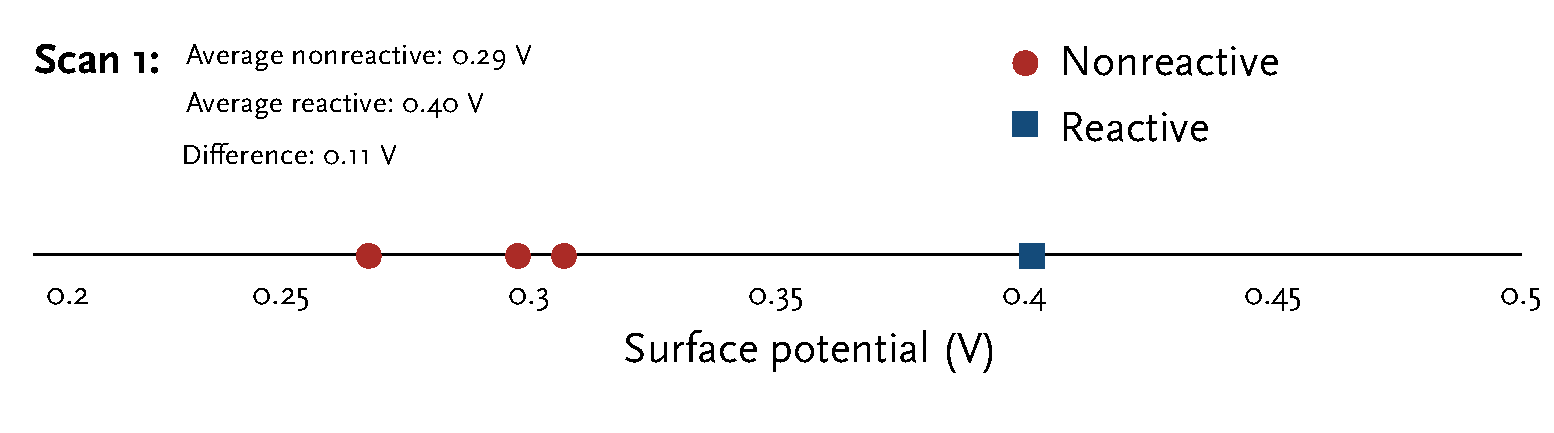
\includegraphics[width=0.8\textwidth]{Scan1.pdf} \\ 
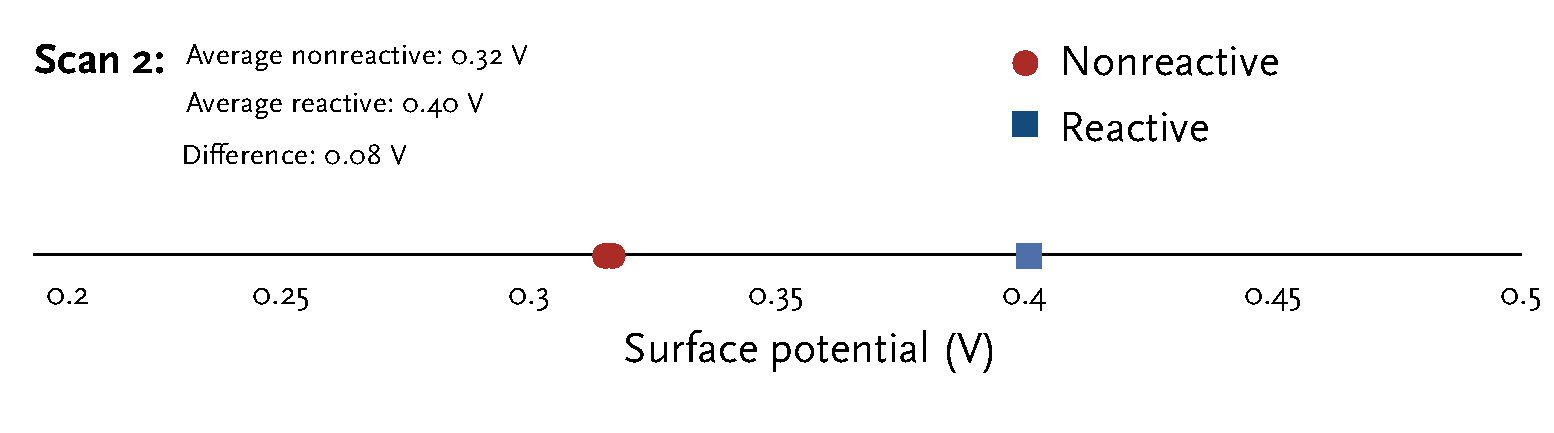
\includegraphics[width=0.8\textwidth]{Scan2.pdf} \\ 
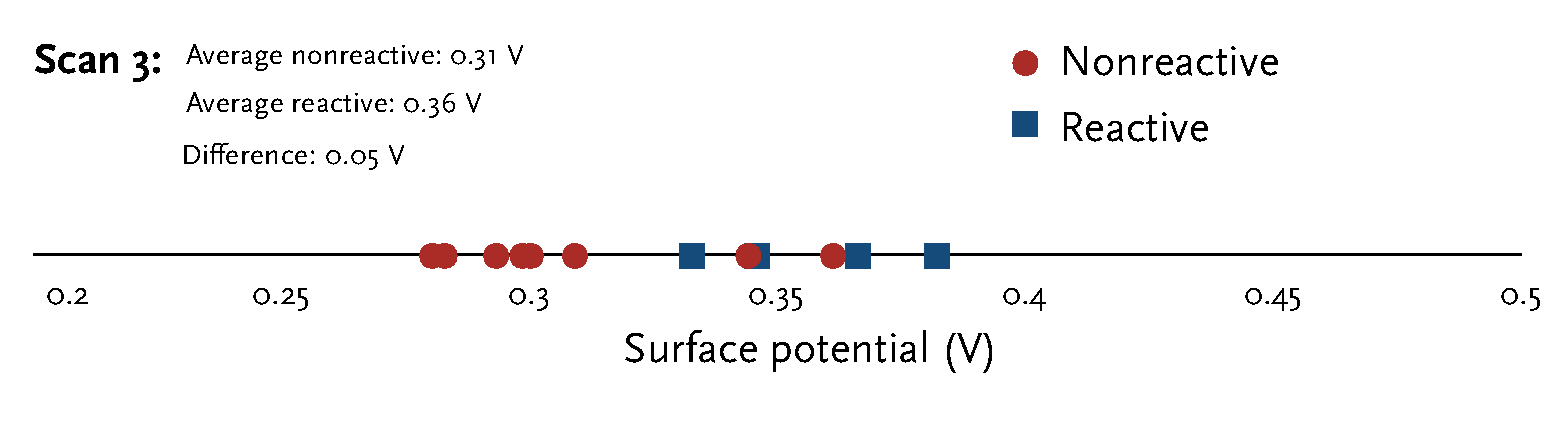
\includegraphics[width=0.8\textwidth]{Scan3.pdf} \\ 
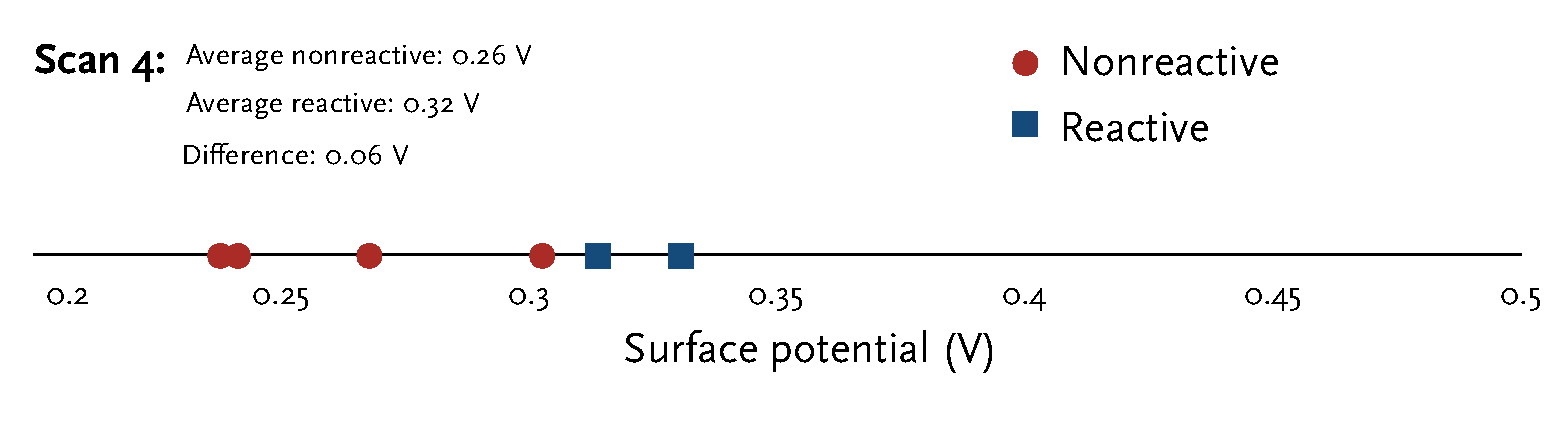
\includegraphics[width=0.8\textwidth]{Scan4.pdf} \\ 
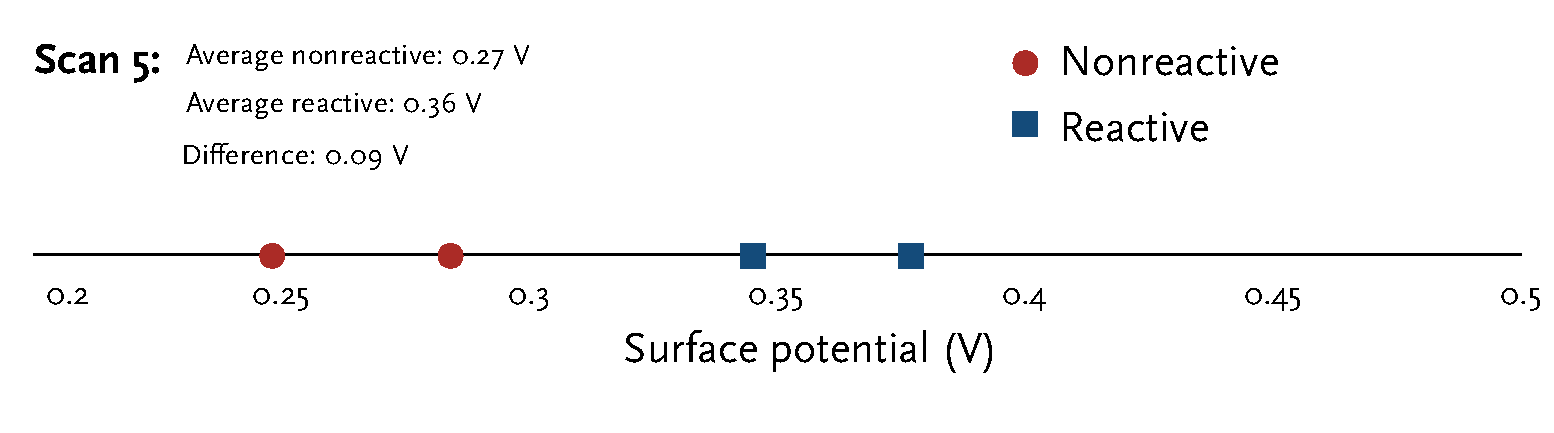
\includegraphics[width=0.8\textwidth]{Scan5.pdf} \\ 
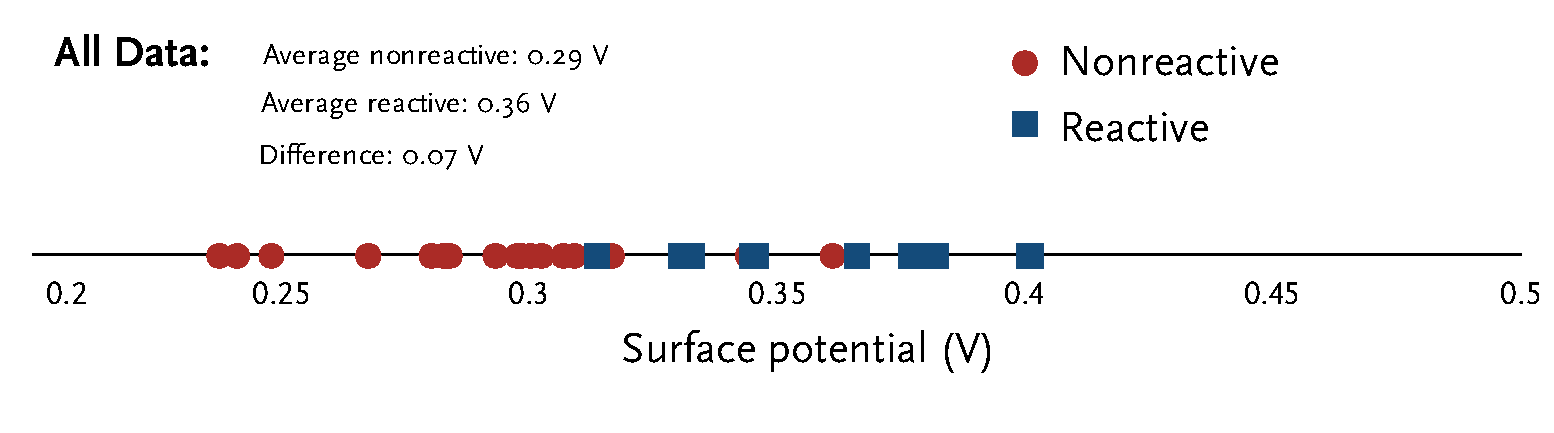
\includegraphics[width=0.8\textwidth]{AllData.pdf}
\end{array}$
\caption[Average surface potential for each grain]{Plots of the average surface potential
for each grain within each scan, as well as the amalgamated data from all scans. Reactive
grains appear as blue boxes and nonreactive grains appear as read circles on the plots.
With two exceptions, the grains with the highest surface potential in each scan were the
most reactive. The average difference in surface potential between reactive and
nonreactive grains was \SI{70}{\milli\volt}.}
\label{fig:fe2o3kfmplots}
\end{figure}
On average, reactive grains had a surface potential \SI{70}{\milli\volt} higher than
nonreactive grains. The correlation between highly reactive grains and a higher surface
potential was clear for all scans. With only a few exceptions, the grains with the highest
surface potential within each scan were the reactive grains.

\section{Discussion}\label{sec:ch9discussion}

The data show that hematite polycrystals exhibit extremely anisotropic photochemical
activity. Grains oriented near the (1\={2}10) orientation are significantly more reactive
than other grains at the surface. This remains true both under ultraviolet and visible
light illumination. \abbr{AFM} images suggest that this is unrelated to the presence of
facets at the surface. Both faceted and nonfaceted grains were observed to be reactive or
nonreactive.

Earlier studies of photochemical anisotropic behavior of oxide polycrystals have
attributed the effect to both surface and bulk properties. For example, Giocondi et
al.\cite{Giocondi:2007fa} attributed the photochemical activity of \ce{SrTiO3}
polycrystals to differences in the energy levels of the band dispersion. The authors
suggested that higher rates of reactivity were the result of an increased generation of
carriers with momentum along certain crystal directions. On the other hand, Lowekamp et
al.\cite{Lowekamp:1998ks} suggest that the increased reactivity of \ce{TiO2} polycrystals
arises from the presence of highly active surface planes, rather than from a bulk
property. Because of the lack of conclusive evidence supporting the bulk or surface cause
of anisotropic photochemical reactivity for oxide polycrystals, both possibilities will be
examined here.

For hexagonal crystal systems, studies of anisotropic properties often focus on property
differences between basal and prismatic planes. The basal plane is defined as the plane
perpendicular to the c-axis of the unit cell. The prismatic planes are the set of planes
parallel to the c-axis, intersecting the a-axis directions of the unit cell. For example,
in corundum-type materials, which includes \textalpha-\ce{Fe2O3}, the structure consists
of close-packed oxygen planes stacked along the c-axis, with \ce{Fe^{3+}} ions filling two
thirds of the interstitial sites. As a result, electron travel within the basal plane
occurs within planes of iron ions, while travel perpendicular to the plane results in
traversing layers basal layers of oxygen ions.\cite{Iordanova:2005ha} As a result,
anisotropic electrical properties have been observed when comparing these
directions.\cite{Benjelloun:1984cq}

For \ce{Fe2O3}, differences in electron conductivity between the basal plane and the
prismatic planes are observed. Conductivity along the c-axis direction in \ce{Fe2O3} is
lower than along perpendicualr directions.\cite{Huda:2010kx,Iordanova:2005ha}
Photochemical experiments determined that the onset of photocurrent for hematite basal
planes is different than that of prismatic planes.\cite{Eggleston:2009ic} Prismatic faces
of the crystal showed an earlier onset of photocurrent than basal planes. That study only
differentiated between properties of the basal plane and the prismatic planes, and did not
study differences in properties between the prismatic faces. The work presented here shows
a strong difference in photochemical properties not only between the basal and prismatic
orientations, but also determined that one prismatic orientation is significantly more
reactive than the others. 

\begin{figure}
\begin{center}
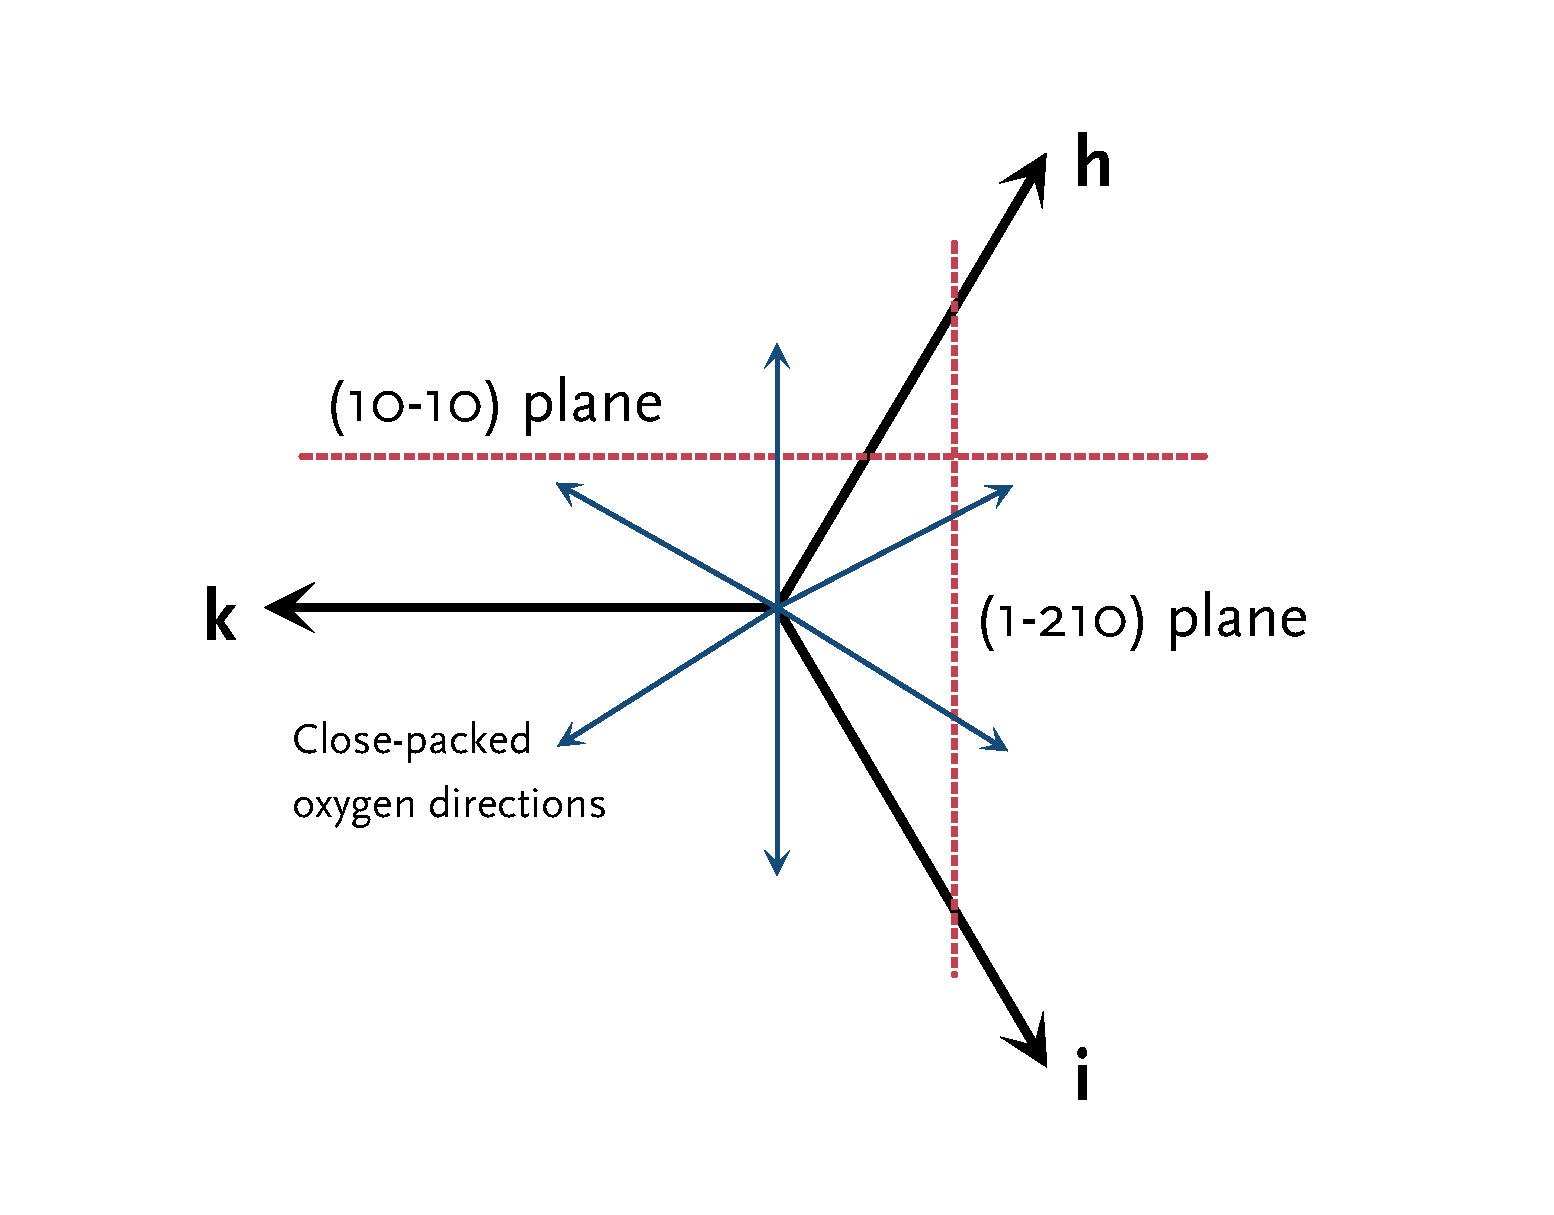
\includegraphics[width=0.6\textwidth]{fe2o3axes.pdf}
\caption[(1\={2}10) and (10\={1}0) planes in relation to in-plane crystal axes]{%
	Schematic showing the (1\={2}10) and (10\={1}0) planes in 
	relation to the in-plane hexagonal crystal axes. Also shown 
	are the close-packed directions of the close packed oxygen 
	network of the basal plane. These close packed directions are 
	located \SI{30}{\degree} from the in-plane crystal axes. The 
	(1\={2}10) planes are perpendicular to the axes of the unit 
	cell, while the (10\={1}0) planes are perpendicular to the 
	close packed directions.
}
\label{fig:fe2o3axes}
\end{center}
\end{figure}
%\sidefigure[(1\={2}10) and (10\={1}0) planes in relation to in-plane crystal axes]{%
%	Schematic showing the (1\={2}10) and (10\={1}0) planes in 
%	relation to the in-plane hexagonal crystal axes. Also shown 
%	are the close-packed directions of the close packed oxygen 
%	network of the basal plane. These close packed directions are 
%	located \SI{30}{\degree} from the in-plane crystal axes. The 
%	(1\={2}10) planes are perpendicular to the axes of the unit 
%	cell, while the (10\={1}0) planes are perpendicular to the 
%	close packed directions.
%	\label{fig:fe2o3axes}
%	}{%
%	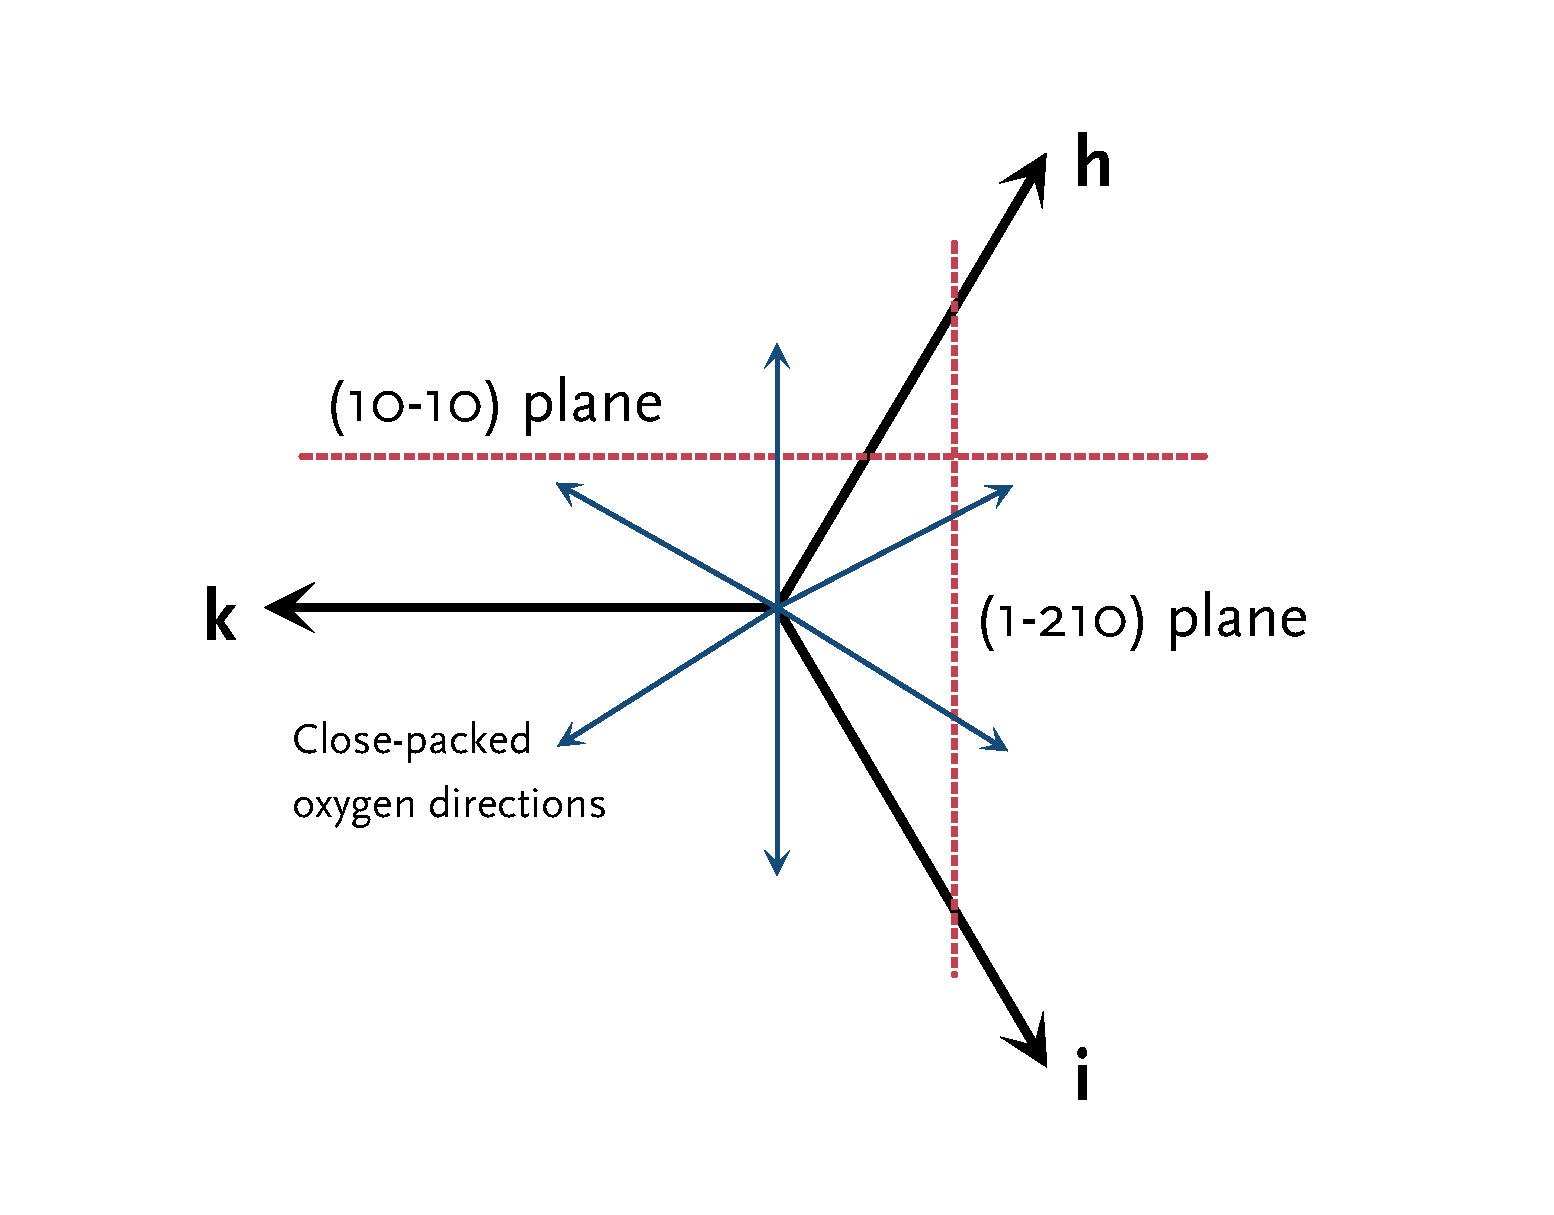
\includegraphics[width=\marginparwidth]{fe2o3axes.pdf}
%}{-20}	
			
The two low-index prismatic orientations  of \ce{Fe2O3} are (in 4-index notation) the
\{1\={2}10\} and the \{10\={1}0\} families. These planes are depicted in
\figureref{fe2o3axes}. Polycrystalline grains near the (1\={2}10) orientation were
significantly more reactive than all other orientations, including the (10\={1}0)
orientation. The data acquired from Kelvin probe force microscopy show that the reactive
orientation are associated with a higher surface potential than the surrounding nonactive
grains. It is logical that grains with a higher surface potential correspond to a higher
reactivity for photochemical reduction reactions, which includes the reduction of aqueous
silver in this work. A more positive potential at the surface would decrease upward or
increase downward band bending at the surface. In this case, reactive grains were an
average of \SI{70}{\milli\volt} more positive than nonreactive grains. 
%The effect of the difference in band bending on photochemical activity is shown
%schematically in the energy level diagram in \figureref{fe2o3bending}.
%\begin{figure}[htbp]
%\begin{center}
%
\includegraphics[width=0.8\textwidth]{fe2o3bending.pdf}
%\caption{Schematic energy level diagram showing the effect of a higher surface potential
%on the band bending and photochemical activity of hematite. The higher surface potential
%decreases upward band bending at the surface of the n-type \ce{Fe2O3}. The reduction in
%upward band bending allows more photogenerated electrons to reach the surface and
%participate in the photochemical reduction of silver ions.}
%\label{fig:fe2o3bending}
%\end{center}
%\end{figure}

An examination of the possible surface terminations of prismatic hematite orientations
gives a possible explanation for the increased reactivity. \figureref{fe2o3terminations}
shows atomic models of the (1\={2}10) and (10\={1}0) planes of \ce{Fe2O3}.
\begin{figure}[htbp]
\begin{center}$
\begin{array}{cc}
\centerline{\includegraphics[width=0.75\textwidth]{1010surface.pdf}} \\ 
\centerline{\includegraphics[width=0.75\textwidth]{1210surface.pdf}}
\end{array}$
\caption[Depiction of the (10\={1}0) and (1\={2}10) terminations of hematite]{Depiction of
the (a) (10\={1}0) and (b) (1\={2}10) terminations of hematite. The (10\={1}0) surface is
terminated by a neutral formula unit. Outlined atoms in (a) represent the neutral
repeating \abbr{2D} unit cell. The (1\={2}10) surface is terminated by a polar termination
of either a layer of iron atoms or oxygen atoms. (c) Side view of the (1\={2}10) surface,
showing alternating layers of O or Fe atoms.}
\label{fig:fe2o3terminations}
\end{center}
\end{figure}
The (10\={1}0) is neutral, terminated by a formula unit of \ce{Fe^{3+}} and \ce{O^{2-}}
ions. On the other hand, the (1\={2}10) surface is terminated by alternating layers of
\ce{O^{2-}} and \ce{Fe^{3+}}. For \ce{Fe2O3} films on single crystal substrates presented
in the following chapter, polar surface terminations are present in the more reactive
case. The basal plane is also terminated by polar planes, but as already stated, mobility
along the c-axis is low, which would account for lack of active orientations along this
direction.

\begin{figure}
    \begin{center}
    \includegraphics[width=0.6\textwidth]{fe2o3dispersion.pdf}
    \caption[Calculated hematite band electronic band structure]{%
        Calculated hematite band electronic band structure. The bands were reproduced from
        Huda et al.,\cite{Huda:2010kx} but have been rigidly shifted to reflect the experimentally
        observed band gap. The shaded region represents the momentum states where vertical
        transitions are possible with the energy of light from the blue \abbr{LED} used in these
        experiments.}
    \label{fig:fe2o3dispersion}
    \end{center}
\end{figure}
%\sidefigure[Calculated hematite band electronic band structure]{%
%	Calculated hematite band electronic band structure, reproduced from reference
%\citet{Huda:2010kx}.
%	\label{fig:fe2o3dispersion}
%	}{%
%	\includegraphics[width=\marginparwidth]{fe2o3dispersion.pdf}
%}{0}	
Giocondi et al.\cite{Giocondi:2007fa} hypothesized that differences in photochemical
reactivity of \ce{SrTiO3} arise from preferred charge carrier generation along certain
crystallographic directions. \figureref{fe2o3dispersion} presents a calculated band
dispersion for hematite \ce{Fe2O3}. For hexagonal crystals, {\textGamma} represents the
center of the Brillouin zone. \textGamma$\rightarrow${\textAlpha} represents charge
carriers generated along the c-axis direction (parallel to the [0001] direction).
\textGamma$\rightarrow${\textMu} represents carriers generated perpendicular to the
(1\={2}10) plane (parallel to a prismatic axis). \textGamma$\rightarrow${\textKappa}
represents the generation of carriers perpendicular to the (10\={1}0) orientation,
traveling in a direction \SI{30}{\degree} offset from a prismatic axis, along a close
packed oxygen direction.

The band structure gives another explanation for the low reactivity of (0001) faces of
bulk hematite. The direct band gap for electrons traveling perpendicular to this face is
on the order of 0.3-0.5 \si{\electronvolt} larger than for electrons traveling toward the
prismatic faces. The larger band gap is expected to result in fewer charge carriers
generated in that direction than for the other faces. This is particularly true in the
case of illumination by the wide spectrum Xe lamp, which generates more low energy photons
than the blue \abbr{LED}. However, the band dispersion shows little difference in the band
gap when comparing the M and K points, which correspond to the (1\={2}10) and (10\={1}0)
zones respectively.
%The \SI{470}{\nano\meter} peak of the blue \abbr{LED} corresponds to a photon energy of
%\SI{2.6}{\electronvolt}, which is of sufficient to generate charge carriers in all
%directions. 



\section{Conclusions and Context}\label{sec:ch9conclusion} 

The (1\={2}10) orientated grains of polycrystalline \ce{Fe2O3} are significantly more
reactive than all other orientations, including other low index prismatic orientations.
Reactive grains correspond to grains with a higher surface potential, as determined
through Kelvin probe force microscopy. The anisotropy in photochemical activity is the
same for reactions performed under wide spectrum light including ultraviolet light as well
as for narrow spectrum visible light from a blue \abbr{LED}. The reactive orientation
corresponds to a prismatic direction terminated by polar surface planes with a significant
number of low energy electrons having momentum in that direction. 

In the context of the other work presented in this document, these results serve to
clarify some of the complicated results presented in later chapters and introduce the
effect of polar surface terminations on photochemical reactivity. This work provides 
information on base reactivity of bulk, polycrystalline hematite. It also correlates
reactivity with grain orientation. These results provide a context for future results. 
For example, for bulk hematite, the c-axis (0001) orientation is consistently not as 
reactive as the (1\={2}10) face, and orientation is not a key factor driving the results 
for films on single crystals presented in \chapterref{single.crystal.reactivity}. Similar 
interpretations can be applied to the results for films on polycrystalline substrates 
presented in \chapterref{polycrystalline.reactivity}. 
		% !TEX root = base.tex 

\chapter{Hematite Reactivity on Single Crystal Substrates}
\label{ch:single.crystal.reactivity}


\chintro{The majority of the text in this chapter appears in \emph{Chemical
Communications}, 2012, 48 (14), 2012-2014.\cite{Schultz:2012cr} This chapter describes the
reactivity of thin films of \textalpha-\ce{Fe2O3} on various single crystal substrates.
The key discovery reported in this section is that thin films of \textalpha-\ce{Fe2O3}
show drastically differing levels of photochemical reactivity when supported on different
substrates. (0001)-oriented \ce{Fe2O3} on (111)-oriented \ce{SrTiO3} substrates are
significantly more reactive than films supported on (0001)-\ce{Al2O3} or even bulk
polycrystalline \ce{Fe2O3}. Previous work in the \ce{SrTiO3}/\ce{Fe2O3} system has focused 
on improving the activity of \ce{SrTiO3} through the incorporation of \ce{Fe2O3} as an electron
scavenger.\cite{Luo:2006kg,Wang:2007fp} Those experiments tested the activity of the
heterostructures towards photochemical oxidation (with \ce{SrTiO3} acting as a
photoanode). Here, the behavior of \ce{Fe2O3}/\ce{SrTiO3} heterostructures is tested in
the reverse configuration. \ce{Fe2O3} is the active material, supported on \ce{SrTiO3},
and acts as a photocathode for reducing aqueous \ce{Ag+} to solid Ag.}
 
 
\section{Experimental Details}
\label{sec:single.crystal.experimental}

 
\ce{Fe2O3} films were deposited on various substrates using pulsed laser deposition. Basic
procedures outlined in Chapter~\ref{ch:experimental} were followed for pulsed laser
deposition and synthesis of a polycrystalline hematite target. Films were deposited on
single crystal \ce{SrTiO3} (111) and \ce{Al2O3} (0001) substrates. Both films were
verified as (0001) oriented via X-ray diffraction. Bulk \ce{Fe2O3} was prepared as
described in \S \ref{subsec:exp.solidstate}.


\section{Results}
\label{sec:single.crystal.results}


\figureref{thinfilmresults} shows \abbr{AFM} images of the film surfaces before and after
reaction with the AgNO3 solution.  
\begin{figure}
	\includegraphics[width=\textwidth]{thinfilmresults.pdf}
	\caption[Images of thin film surfaces after reaction]{%
		Topographic \abbr{AFM} images of sample surfaces before (a-c) and 
		after (d-f) the photochemical reduction of Ag from an aqueous 
		\ce{AgNO3} solution. (a) and (d) show the surface of the 
		\ce{Fe2O3} film supported on \ce{Al2O3}, (b) and (e) show 
		the \ce{Fe2O3} film on \ce{SrTiO3}, and (c) and (f) show bulk 
		polycrystalline \ce{Fe2O3}. The arrows next to the micrographs 
		in (d-f) indicate the location of the horizontal line used for 
		\figureref{lineprofiles}.}
	\label{fig:thinfilmresults}
\end{figure}
\figureref{thinfilmresults}(a) and \figureref{thinfilmresults}(b) show the clean surface
of the \ce{Fe2O3} films on \ce{SrTiO3} and \ce{Al2O3}, respectively. 
\figureref{thinfilmresults}(c) shows the clean surface of bulk \ce{Fe2O3}. The
corresponding surfaces after reaction are shown in Figures
\figureref{thinfilmresults}(c)-(e). All areas are \SI{10}{\micro\meter} x
\SI{10}{\micro\meter}, but the vertical scales differ. After reaction, the surface of the
film on alumina, \figureref{thinfilmresults}(d), shows occasional small silver deposits,
visible as bright spots on the micrograph.  The surface of the film on the
\ce{SrTiO3}(111) substrate, shown in \figureref{thinfilmresults}(e), is covered in a
thick, inhomogeneous layer of reaction product.  The amount of silver present after
reaction on the film supported on the \ce{SrTiO3} substrate is much greater than for the
film on alumina or for the bulk sample in \figureref{thinfilmresults}(f).  Of particular
note is the difference in vertical scales for the micrographs after the photochemical
reduction of Ag.  The vertical scale for the reaction on the \ce{SrTiO3} supported film is
\SI{290}{\nano\meter}, as compared to \SI{100}{\nano\meter} and \SI{68}{\nano\meter} for
the film on alumina and the bulk hematite, respectively. The (0001) oriented film on
\ce{SrTiO3} is significantly more reactive than the (0001) grains observed for bulk
\ce{Fe2O3}, reported in \chapterref{fe2o3orientation}.

\begin{figure}
\begin{center}
\includegraphics[width=0.8\textwidth]{lineprofiles.pdf}
\caption[Line profiles from \figureref{thinfilmresults}]{%
	Topography along lines from the \abbr{AFM} micrographs in \figureref{thinfilmresults}.

	The arrows next to the micrographs in \figureref{thinfilmresults}(d)-(f) 
	indicate the location of the horizontal line used for \figureref{lineprofiles}.}
\label{fig:lineprofiles}
\end{center}
\end{figure}
%\sidefigure[Line profiles from \figureref{thinfilmresults}]{%
%	Topography along lines from the \abbr{AFM} micrographs in
\figureref{thinfilmresults}. 
%	The arrows next to the micrographs in \figureref{thinfilmresults}(d)-(f) 
%	indicate the location of the horizontal line used for \figureref{lineprofiles}.
%	\label{fig:lineprofiles}
%	}{%
%	\includegraphics[width=\marginparwidth]{lineprofiles.pdf}
%}{0}
The differences in the heights of the Ag on the three surfaces are shown quantitatively in
\figureref{lineprofiles}, which compares the topography along lines from the three
micrographs in \figureref{thinfilmresults}(d)-(f). The heights of the Ag deposits on the
\textalpha-\ce{Fe2O3}/\ce{SrTiO3}(111) heterostructure range from 100 to
\SI{250}{\nano\meter}.  On the other two surfaces, all of the deposits are less than
\SI{100}{\nano\meter}.  The images in \figureref{thinfilmresults} are characteristic of
all areas that were examined.

The results presented in this chapter were consistently observed over multiple samples. In
all cases, the film on \ce{SrTiO3}(111) was significantly more reactive than the film on
alumina. The reactivity difference was so extreme that it could be used to visually
distinguish the films after reaction. After longer reaction times (on the scale of minutes
to an hour), the entire surface of the film supported on \ce{SrTiO3}(111) was covered with
silver reaction product, and excess silver was visible floating in the reaction solution.
On the film on alumina after the same reaction time, little to no reaction product could
be observed with the naked eye.


\section{Discussion}
\label{sec:single.crystal.discussion}


The results presented in \figureref{thinfilmresults} and \figureref{lineprofiles}
demonstrate that the \textalpha-\ce{Fe2O3} film on \ce{SrTiO3}(111) has a much higher
photochemical reactivity for the reduction of silver ions than a comparable film on
\ce{Al2O3} and even bulk hematite.  The images in \figureref{thinfilmresults} reveal that
the film on \ce{SrTiO3} has the greatest silver surface coverage. The data in
\figureref{lineprofiles} show that the silver deposits are larger for films on \ce{SrTiO3}
than for films on alumina or for bulk \ce{Fe2O3}. 

This result is surprising for multiple reasons.  The structure of both films does not vary
enough to cause the marked difference in reactivity. Both films are (0001)-oriented
\textalpha-\ce{Fe2O3} of nominally equal thickness.  \abbr{AFM} scans show that the
morphology of the films is similar. The thickness of the films used in this experiment was
\texttildelow\SI{50}{\nano\meter}. Based solely on the depth of light absorption in
\ce{Fe2O3}, one could expect the bulk sample to be much more reactive than the films.  The
penetration depth of \SI{470}{\nano\meter} photons in hematite reported to be
approximately \SI{450}{\nano\meter}.\cite{Marusak:1980gc}  The films were of a sufficient
thickness to absorb only a fraction of the incident light, in contrast to the bulk sample,
which was much thicker than the absorption depth. Furthermore, based on the index of
refraction mismatch, the \ce{Al2O3}/\ce{Fe2O3} interface is more reflective than the
\ce{SrTiO3}/\ce{Fe2O3} interface, so internal reflection leading to an increase in path
length in the film cannot account for the difference in reactivity.  In both cases, the
band gap of the substrate (> \SI{8}{\electronvolt} for \ce{Al2O3},\cite{French:1998wj} and
\SI{3.2}{\electronvolt}  for \ce{SrTiO3}\cite{Cardona:1965vw}) is too large for the light
used in this experiment to generate a significant number of electron-hole pairs.  We can
therefore conclude that the majority of the electron hole pairs were generated in the
films. Neither substrate was able to participate in photochemical reactions by absorbing
light and shuttling generated charge carriers to the surface of the film, as seen in
previous experiments with UV light and \ce{TiO2}/\ce{BaTiO3}
heterostructures.\cite{Burbure:2010ti,Burbure:2010go}  Despite the fact that it absorbs
less light, the film supported by \ce{SrTiO3} was more reactive than the bulk sample.

One possible explanation for the increased reactivity of the film supported on \ce{SrTiO3}
lies in the band structure of the substrate materials. Previous authors investigating the
\ce{SrTiO3}/\ce{Fe2O3} system have suggested that the \ce{Fe2O3} layer acts as an electron
acceptor transferring holes to the active \ce{SrTiO3} photoanode.\cite{Wang:2007fp} If
\ce{Fe2O3} acts as a sink for electrons at the back of the active layer, more holes can
reach the surface without recombining.  One could make the reverse argument here to
explain the current observations.  In this case, the \ce{SrTiO3} layer can act as a hole
acceptor, increasing the number of photogenerated electrons that reach the \ce{Fe2O3}
surface to participate in the photocathodic reaction.  This could explain why the thin
film sample has a much higher reactivity than the bulk material, even though less light is
absorbed.  Because the band gap of alumina is significantly larger than that of the
\ce{Fe2O3} film, there exists a significant barrier to charge transfer across the
interface.  As a result, the alumina substrate cannot accept holes, and the recombination
rate within the film is not decreased.

Assuming \ce{SrTiO3} acts as a hole acceptor and this is responsible for the increased
reactivity, we must also consider what happens to these holes.  In our experimental
set-up, there is no path to ground or to complete the circuit with the solution.  If the
holes were to build up in the substrate, the heterostructure would become charged and the
reaction would stop.

A second explanation is that uncompensated charge at the \ce{SrTiO3}(111) acts to separate
electrons and holes, reducing recombination.  The individual (111) atomic planes in the
\ce{SrTiO3} structure have alternate positive (\ce{Ti^{4+}}) and negative charges
(\ce{SrO3^{4-}}).  Terminating the surface in a single charge is energetically costly, so
the surface breaks up into positive domains with Ti termination and negative domains with
\ce{SrO3} termination.  Giocondi\cite{Giocondi:2003wc} has shown that the oppositely
charge surface domains have different photochemical properties, with one favoring
reduction and the other favoring oxidation.  Note that \textalpha-\ce{Fe2O3} also has
planes of alternating charge parallel to the interfaces plane.  However, the trivalent
charges of the (0001) planes cannot completely compensate the charge from the
\ce{SrTiO3}(111) surface.  These charges can, however, exactly compensate the charges on
the isostructural, isoelectronic \ce{Al2O3}(0001) surface.
\begin{figure}
\begin{center}
\includegraphics[width=0.6\textwidth]{polarterms.pdf}
\caption[Charges at internal interface between \ce{SrTiO3} and \ce{Fe2O3}]{%
		Schematic depiction of the charges at the internal interface 
		between \ce{SrTiO3}(111) and \textalpha-\ce{Fe2O3}. There are 
		alternating planes of charge along the [111] direction and some 
		areas are positively terminated (upper) and others have a negative 
		termination (lower). The charged termination will cause the bands 
		in the film to bend in a way that will move carriers in opposite 
		direction. E$_C$ and E$_V$ label the conduction and valence band 
		edges, respectively.}
\label{fig:polarterms}
\end{center}
\end{figure}
%\sidefigure[Charges at internal interface between \ce{SrTiO3} and \ce{Fe2O3}]{%
%		Schematic depiction of the charges at the internal interface 
%		between \ce{SrTiO3}(111) and \textalpha-\ce{Fe2O3}. There are 
%		alternating planes of charge along the [111] direction and some 
%		areas are positively terminated (upper) and others have a negative 
%		termination (lower). The charged termination will cause the bands 
%		in the film to bend in a way that will move carriers in opposite 
%		direction. E$_C$ and E$_V$ label the conduction and valence band 
%		edges, respectively.
%	\label{fig:polarterms}
%	}{%
%	\includegraphics[width=\marginparwidth]{polarterms.pdf}
%}{-4}
\figureref{polarterms} illustrates a schematic view of our proposed explanation for the
enhanced reactivity of \textalpha-\ce{Fe2O3}/\ce{SrTiO3}(111) heterostructures. In the
hematite film above positively terminated domains, bands bend downward and draw
photogenerated electrons to the internal interface while holes are drawn to the
hematite/solution interface.  The opposite occurs in negative domains and this is where
the reduction of silver occurs.  In each case, the complementary carriers can recombine
within \ce{SrTiO3}, so there is no charge accumulation.  Note that the previous work
showed that charged domains on the \ce{SrTiO3}(111) surface have dimensions on the order
1-2~\si{\micro\meter} (refer to \figureref{giocondi}).  This may account for the highly
heterogeneous distribution of Ag on the surface of the heterostructure in
\figureref{thinfilmresults}(e).

Finally, it is noted that the lattice parameter mismatch is significantly larger for 
films on alumina than films on \ce{SrTiO3}. The mismatch between the 
a-axis lattice parameter for \ce{Fe2O3} and the atomic spacing of 
(111)-\ce{SrTiO3} is 3.2\%. The mismatch between alumina and hematite is 
\texttildelow{}20\%. As a result, the films on alumina are expected to 
have a much higher defect concentration than films on \ce{SrTiO3}. 
Defects are known to act as recombination sites for charge carriers. 
The higher concentration of defects in the film on alumina could help 
explain the low activity of this film.


\section{Conclusions}
\label{sec:single.crystal.conclusions}


In summary, \ce{Fe2O3} films on \ce{SrTiO3} substrates show greatly enhanced reactivity
when compared to films on \ce{Al2O3} substrates. The reactivities of \ce{SrTiO3} supported
films are also greater than the reactivity of bulk \ce{Fe2O3} samples.  The results show
that the visible light photochemical activity of hematite, \textalpha-\ce{Fe2O3}, can be
enhanced through the proper choice of substrate material. If polar terminations of the
\ce{SrTiO3}(111) surface are responsible for the increased reactivity, then the enhanced
reactivity of the heterostructure should not occur on nonpolar substrate orientations. 
For example, the \ce{SrTiO3}(100) surface is nonpolar and does not have charged domains or
spatially selective reactivity.\cite{Giocondi:2003wc} Results of photochemical activity of
\ce{Fe2O3} films on polycrystalline perovskite substrates are included later in this
document.
		% !TEX root = base.tex 

\chapter{Hematite Film Reactivity on Polycrystalline Substrates}
\label{ch:polycrystalline.reactivity}


\chintro{This chapter reports on the photochemical activity of the hematite films supported on polycrystalline \ce{SrTiO3} substrates. The area examined for reactivity experiments was the same area used to determine the orientation relationships, discussed later in \chapterref{polycrystalline.growth}. After reaction with the silver nitrate solution, the reactivity of film grains was correlated to substrate and film reactivity.}


\section{Experimental Details}
\label{sec:poly.reac.experimental}


The photochemical activity of \ce{Fe2O3} films grown on polycrystalline \ce{SrTiO3} substrates is reported in this chapter. An analysis of film growth and orientation relationships is reported later in \chapterref{polycrystalline.growth}. Details on film growth can be found in \sectionpageref{sec:poly.growth.experimental}. Electron backscatter diffraction (\abbr{EBSD}) data from \figureref{subfilmmaps} was used to correlate reactivity with orientation. Details for data collection can be found in \sectionpageref{sec:poly.growth.experimental}. Before the removal of the film to analyze substrate grain orientations, the photochemical marker reaction was performed on the film and analyzed using optical and atomic force microscopy (\abbr{AFM}). Marker reactions were performed as described in \sectionpageref{subsec:exp.markerreactions}. The light source was a blue \abbr{LED}, and the reaction time was one minute. This time was selected after trials with reaction times, and was found to result in some grains that were bare, while other grains were highly reactive. Longer reaction times resulted in the entire surface covered in reaction product. After these longer reaction times, silver colored material visibly coated the reaction surface, without the aid of microscope analysis. Because the light source was the \abbr{LED}, only visible light was available to excite electrons to the conduction band. Because the band gap of \ce{SrTiO3} requires ultraviolet light to generate charge carriers, all photochemical activity was attributed to the film. It was assumed that a negligible number of charge carriers were generated in the substrate.

\section{Results}
\label{sec:poly.reac.results}

After reaction with the silver nitrate solution, the film was examined using optical and atomic force microscopy. Optical microscopy provided a rapid, high throughput classification of the entire area. \abbr{AFM} then confirmed the interpretation of the optical micrograph, and provided a detailed look at small subsections of the examined area.


\subsection{Optical Microscopy}
\label{subsec:poly.reac.optical}


\figureref{filmoptical} shows an optical micrograph of an area of the sample surface after reaction. Dark areas on the micrograph generally indicate areas with a large amount of reaction product. Pores are also responsible for some areas of dark contrast. Any pores could be identified by comparison with an image of the clean sample surface. The image of the clean surface also served as a reference, verifying that dark contrast was not present. The clean surface is uniformly bright, with the exception of pores, cracks, and grain boundaries. These areas appear as dark spots on the micrograph. Some grains appear slightly darker than others. This is a result of differing interaction with the polarized light, and does not represent reaction product on the surface. \figureref{filmclean} shows the surface after reaction product was cleaned, for comparison with the image in \figureref{filmoptical}.
\begin{figure}
	\includegraphics[width=0.8\textwidth]{filmoptical.pdf}
		\caption[Film surface after reaction]{%
			Surface of \ce{Fe2O3} film on polycrystalline
			\ce{SrTiO3} substrate after marker reaction. Areas
			of dark contrast correspond to portions of the surface
			covered with a large amount of reaction product.
			Bright areas are bare areas, with little reaction
			product.}
	\label{fig:filmoptical}
\end{figure}
%
%
\begin{figure}
\begin{center}
\includegraphics[width=0.8\textwidth]{filmclean.jpg}
\caption[Cleaned film surface]{%
	Surface of \ce{Fe2O3} film on polycrystalline \ce{SrTiO3} 
	substrate after cleaning. The surface shows uniform contrast, exception pores, cracks, and the affect of light polarization,
	supporting the interpretation of contrast in \figureref{filmoptical}.}
\label{fig:filmclean}
\end{center}
\end{figure}
%\sidefigure[Cleaned film surface.]{%
%	Surface of \ce{Fe2O3} film on polycrystalline \ce{SrTiO3} 
%	substrate after cleaning. The surface shows uniform contrast,
%	supporting the interpretation of contrast in \figureref{filmoptical}.
%	\label{fig:filmclean}
%	}{%
%	\includegraphics[width=\marginparwidth]{filmclean.jpg}
%}{0} % Last argument is number of lines to move up or down

Using the electron backscatter diffraction maps in \figureref{subfilmmaps} as a guide, each individual film grain was identified in the optical image in \figureref{filmoptical}. The identified grains were manually classified as highly reactive, moderately reactive, or nonreactive. Grains that were uniformly dark were classified as highly reactive. Conversely, grains that were uniformly bright were nonreactive. Grains that appeared a medium gray color, or were otherwise not uniformly covered by reaction product were labelled moderately reactive.

\figureref{labeledgrains} shows a digram of the resulting classifications. The grain boundaries were taken from the \abbr{EBSD} map of the substrate. Dark blue portions of this map correspond to highly reactive grains, medium blue to moderately reactive grains, and light blue areas are nonreactive grains. White corresponds to areas where no assignment was made. This occurred when it was unclear the reactivity level of a grain, owing to image artifacts or difficulty distinguishing grains. Also, some white grains in \figureref{labeledgrains} were outside the field of view of the microscope image in \figureref{filmclean}.
\begin{figure}
	\includegraphics[width=\textwidth]{labeledgrains.pdf}
		\caption[Reactivity assignments for film]{%
			Grain boundary network taken from \abbr{EBSD} data in 
			\figureref{subfilmmaps}(b) with assignments of reactivity
			observed in \figureref{filmclean}. Dark blue represents 
			highly reactive grains, medium blue represents moderately
			reactive grains, and light blue represents nonreactive 
			grains. White grains are those that were not assigned a 
			reactivity level.}
	\label{fig:labeledgrains}
\end{figure}

The orientation of the substrate and film grains was plotted on the standard stereographic triangles for cubic and hexagonal crystal structures respectively. These plots are depicted in \figureref{substrateplot} and \ref{fig:filmplots}. Both film and substrate orientations were examined to determine whether any reactivity differences were a result of substrate or film orientation alone, or a combination of the two.

\begin{figure}
	\begin{center}
	\includegraphics[width=0.6\textwidth]{substrateplot.pdf}
	\caption[Orientation of substrate grains]{%
	Standard cubic stereographic triangle showing the orientation of
	substrate grains classified in \figureref{labeledgrains}. Dark points are
	highly reactive grains, light points are moderately reactive grains,
	and empty points are nonreactive grains.}
	\label{fig:substrateplot}
	\end{center}
\end{figure}
%\sidefigure[Orientation of substrate grains]{%
%	Standard stereographic triangle showing the orientation of
%	grains classified in \figureref{labeledgrains}. Dark points are
%	highly reactive grains, light points are moderately reactive grains,
%	and empty points are nonreactive grains.
%	\label{fig:substrateplot}
%	}{%
%	\includegraphics[width=\marginparwidth]{substrateplot.pdf}
%}{-8} % Last argument is number of lines to move up or down
In the plot of the substrate grains in \figureref{substrateplot}, highly reactive grains are represented by dark points, moderately reactive grains by light points, and nonreactive grains by empty points. The figure doesn't show a strong relation between substrate orientation and grain reactivity. Highly reactive and moderately reactive points are spread throughout the standard stereographic triangle. Nonreactive grains are weakly clustered near the (111) orientation and along the axis between the (001) and (101) orientations.

The reactivity of the film grains are plotted on the three hexagonal triangles in \figureref{filmplots}. 
\begin{figure}2
	\includegraphics[width=\textwidth]{filmplots.pdf}
		\caption[Orientation of film grains]{%
			Standard stereographic triangles showing the orientation
			of (a) highly reactive (dark points), (b) moderately reactive
			(light points), and (c) nonreactive grains (empty points).}
	\label{fig:filmplots}

\end{figure}
The points are plotted in separate triangles to better illustrate trends in the data. Because of the large number of film grains, with each substrate grain supporting multiple film grains,\footnote{For more information on film growth, see \chapterpageref{polycrystalline.growth}.} plotting all data on the same triangle obscures analysis. When all points are on the same triangle, it becomes difficult to observe individual points. The range of orientations contained in this film does not cover the entire stereographic triangle. \figureref{filmplots} shows the entire range of orientations for the film grains on this sample. Grains that were labeled moderately reactive are scattered throughout the entire orientation spread. No clear orientation preference is observed. When examining the plots for highly reactive and nonreactive grains, the situation becomes more complicated. Highly reactive grains are clustered along axis between the (0001) and (1\={2}13) orientations. Conversely, nonreactive grains are clustered near the (0001) orientation and near the axis between (0001) and (0\={1}12)/(10\={1}2) orientations. This suggests and orientation preference for \ce{Fe2O3} films on polycrystalline \ce{SrTiO3} substrates. This is discussed further in \sectionref{sec:poly.reac.discussion}.


\subsection{Atomic Force Microscopy}
\label{subsec:poly.reac.afm}


After optical microscopy, \abbr{AFM} was then used to confirm the interpretation of the optical image. Five individual areas of the sample surface were scanned, each comprising multiple substrate grains. These areas were selected to contain all reactivity classes and a variety of substrate orientations. Representative \abbr{AFM} micrographs of the examined areas are shown in \figureref{filmafm}.
\begin{figure}
\centering
	\includegraphics[width=0.8\textwidth]{filmafm.pdf}
		\caption[Representative \abbr{AFM} images of film]{%
			Representative \abbr{AFM} images of the film surface after
			reaction, showing highly reactive and nonreactive grains.}
	\label{fig:filmafm}
\end{figure}
Reaction product appears as bright contrast in the \abbr{AFM} images. Varying levels of reactivity are seen in each of the micrographs. In \figureref{filmafm}(a), grains identified as highly reactive are outlined.

The \abbr{AFM} micrographs verify the interpretation of the optical images. Grains that were dark on the optical micrograph were the grains with the largest amount of silver product on the surface. Grains that were bright on the optical image had the least amount of reaction product. These results verify the broader but less detailed results from the optical micrograph, and give increased reliability to the reactivity assignments in \figureref{labeledgrains}. \abbr{AFM} analysis did not show a difference in roughness between grains to account for the order of magnitude reactivity difference observed in these results.


\section{Discussion}
\label{sec:poly.reac.discussion}


Overall, the film is more reactive than the bulk hematite. Grains with orientations that demonstrated low reactivity in the bulk were highly reactive in the film. For similar reaction times, the film showed more reactive grains than the bulk, as well as more reaction product on the surface. Especially considering that the film is only \SI{50}{\nano\meter} thick, and so is only absorbing a small portion of the incident light before the interface with the substrate,\footnote{The penetration depth of the light in this experiment (\textlambda = \si{470}{\nano\meter}), reported in \sectionref{sec:single.crystal.discussion}, is \texttildelow\SI{450}{\nano\meter}, significantly larger than the thickness of the film in this experiment.} the film exhibits high reactivity when compared to bulk \ce{Fe2O3}. Once again, the \ce{SrTiO3} substrate improves the photochemical activity of hematite films when compared to the bulk material.

The observed trends in photochemical reactivity in this chapter represent combined effects from \ce{Fe2O3} orientation and substrate/film interaction, each presented the previous to chapters. In \chapterref{fe2o3orientation}, it was observed that \ce{Fe2O3} reactivity is highly anisotropic, with c-axis oriented crystallites showing low reactivity. Conversely, the c-axis oriented films on \ce{SrTiO3} substrates presented in \chapterref{single.crystal.reactivity} were highly reactive. The films on polycrystalline substrates observed here expose varying film orientations while retaining the orientation relationship between film and substrate observed for the films in \chapterref{single.crystal.reactivity}.\footnote{A complete description of the orientation relationship for \ce{Fe2O3} films on polycrystalline \ce{SrTiO3} substrates can be found in \chapterpageref{polycrystalline.growth}.}.

The optical micrograph presented in \figureref{filmoptical} shows clear signs of reactivity differences between grains. Some grains are dark, completely covered in silver reaction product. Other grains are completely devoid of reaction product. The boundaries between areas of high reactivity and low reactivity correlate with \abbr{EBSD} maps of the substrate grains. Qualitatively, the \ce{Fe2O3} film on the \ce{SrTiO3} substrate is overall significantly more reactive than the polycrystalline sample discussed in \chapterref{fe2o3orientation}. 

The results presented in Figures \ref{fig:substrateplot} and \ref{fig:filmplots} suggest that while the film orientation has an effect on reactivity, the substrate orientation does not. Only the mild clustering of non reactive grains found along the axis between (001) and (101) oriented grains suggests any direct affect of substrate orientation on reactivity. On the other hand, the plots for highly reactive, moderately reactive, and nonreactive films differ from each other. Highly reactive grains are clustered along the center of the standard stereographic triangle, along the axis between (0001) and (1\={2}10). Areas along the edge of the triangle, located at orientations between (0001) and (10\={1}0) do have few active grains. The reverse distribution is seen for the nonreactive grains. Nonreactive grains are clustered near the (0001) orientation, and along the axes between (0001) and (0\={1}10)/(10\={1}0). Grains described as moderately reactive were spread over the entire space of film orientations. 

The results here show similar trends to the anisotropic behavior of bulk hematite crystallites.%
\footnote{%
	The discussion in this chapter is a brief overview of the results for photochemical activity of bulk hematite polycrystals. See \chapterpageref{fe2o3orientation} for a detailed description of the results of this experiment.
} 
It is shown in this document that bulk \ce{Fe2O3} grains located near the (1\={2}10) orientation are the most reactive. Grains far away from this orientation exhibited negligible reactivity. This includes (0001) (c-axis) oriented grains, and also grains at any degree of tilt away from (0001) orientation with the [10\={1}0] direction located out of the sample plane. 

For bulk hematite, the grains that were the most reactive were located relatively near to to the (1\={2}10) orientation. The reactive grains in \figureref{filmplots}(a) are tilted considerably closer to (0001) than any of the reactive grains in that study. However, the results here do follow the general trend observed for that work; hematite grains become reactive as they tilt away from the (0001) orientation, \emph{so long as the [1\={2}10] direction is pointing out of the surface}. In other words, if the axis of rotation away from (0001) is a [10\={1}0] direction, the [1\={2}10] direction will be pointing out of the surface, and the grain is likely to be reactive.\footnote{\figurepageref{fe2o3axes} provides a helpful schematic of the relative orientation of the [10\={1}0] and [1\={2}10] directions and planes in the hematite crystal system.} If the tilt axis is the [1\={2}10] direction, the grain is not likely to be reactive, as the orientation will lie along the nonreactive region between (0001) and (10\={1}0). The results for the film materials show the same trend, however the film becomes reactive and a much lower tilt away from (0001). Compare the distribution of reactive grains in \figureref{filmplots} to the distribution in Figures \ref{fig:semtriangle} or \ref{fig:afmtriangle} in \chapterref{fe2o3orientation}.

For the films on single crystal substrates in \chapterref{single.crystal.reactivity}, (0001)-oriented films on (111)-oriented substrates were highly reactive. Here, many grains close to this substrate orientation were marked as nonreactive or moderately reactive. The contradictory results can be understood through the anisotropic reactivity of hematite. For all \ce{Fe2O3} films on \ce{SrTiO3} substrates, the reactivity of the film was improved compared to the bulk material. When grown on single crystal substrates, the only film orientation observed is (0001)  basal plane oriented \ce{Fe2O3}. This orientation is nonreactive for bulk crystals. When films are grown on polycrystalline substrates, more reactive \ce{Fe2O3} orientations are exposed to the surface. If single crystal substrates existed that could be used to stabilize the reactive faces of \ce{Fe2O3}, it is expected that those films would be even more reactive than the films in the previous chapter. However, the low-index orientations available for \ce{SrTiO3} substrates do not stabilize such films. The results in this chapter suggest that the anisotropic reactivity of \ce{Fe2O3} overwhelms effects from substrate/film interactions.

And interesting phenomenon observed for this experiment is that reactivity in some cases appears to be different between film grains on the same substrate. One set of grains is sometimes more reactive than the other. Reactivity following the lamellar structure of the film grains is observed in multiple instances in \figureref{filmoptical}. These cases were generally those of moderate reactivity, and all film grains on that substrate grain were plotted as mildly reactive in \figureref{filmplots}. It may be that further refinement in the orientation depends of hematite reactivity could be observed through an analysis of these grains. However the detail of the optical image was not enough to accurately determine which grains followed this reactivity pattern. 

Additionally, \figureref{labeledgrains} suggests that grains with similar levels of reactivity are clustered near each other. The highly reactive grains are all located near each other, as are many of the nonreactive grains. This could suggest that the high reactivity on some parts of the sample is not directly related to individual crystallite orientation. However, the boundaries between highly active grains and nonreactive grains do sharply follow the grain boundaries identified using \abbr{EBSD}. The results presented in this document do not entirely prove that another affect could be responsible for the high reactivity and resulting clustering of reactive grains. However, the clear demarcation in reactivity across grain boundaries suggest that there is some affect related to individual crystallite properties.
 



\section{Conclusions}
\label{sec:poly.reac.conclusions}

Hematite films on polycrystalline substrates showed clear signs of reactivity differences between grains. Substrate orientation does not appear to drive this reactivity difference, except in that it also is responsible for resulting film orientation. The film orientation shows a correlation between orientation and high and low reactivity. Highly reactive grains were found in the region between (0001) and (1\={2}13) on the standard stereographic triangle. Nonreactive grains were clustered near (0001) and in the region between (0001) and (10\={1}2)/(01\={1}2). This pattern is similar to the orientation dependent reactivity observed in \chapterref{fe2o3orientation}. Additionally, the film on average was significantly more reactive than bulk hematite. 


	\part{Experiments on Film Growth}
		% !TEX root = base.tex 


\chapter{Hematite Film Growth on Single Crystal Substrates}
\label{ch:single.crystal.growth}


\chintro{This section describes the results for studies of \ce{Fe2O3} film growth on single crystal substrates. Film orientation and phase determination was carried out using electron backscatter diffraction analysis and x-ray diffraction. Films were grown on \ce{Al2O3} (0001), \ce{SrTiO3} (111), and \ce{SrTiO3} (001) substrates. The films were epitaxial on \ce{Al2O3} and \ce{SrTiO3} (111). The films on \ce{SrTiO3} (001) were polycrystalline, but show significant texture. }


\section{Film Growth on Strontium Titanate (111) Substrates}
\label{sec:single.growth.111}


\figureref{111maps} shows EBSD maps of a film grown on \ce{SrTiO3} (111) substrate. 
\begin{figure}
	\includegraphics[width=\textwidth]{111maps.pdf}
	\caption[EBSD maps for film on \ce{SrTiO3} (111)]{%
		(a) EBSD phase map for an \ce{Fe2O3} film on \ce{SrTiO3} 
		(111). Red points represent hematite grains and green points 
		represent magnetite. (b) An inverse pole map of the same area 
		of the sample, showing only hematite grains. (c) The selection 
		of points used for the generation of pole figures.}
	\label{fig:111maps}
\end{figure}
\figureref{111maps}(a) is a phase map of all recorded points in the scan. During the automated scan, the EBSD software was allowed to assign either magnetite or hematite phase for each recorded pattern. In this map, points indexed as hematite phase appear red, while points indexed as magnetite are green. The red points (hematite) comprise 97.5 percent of the total data, while only 2.5 percent of points were indexed as magnetite (green). Additionally, the points indexed as magnetite don't appear in any perceivable pattern. Instead, they appear to be distributed randomly over the scan area. These two facts together suggest that the magnetite points can be attributed to errors in the EBSD process, such as poor pattern quality, surface contamination, or areas of poor film quality, such as the macroscopic particles resulting from the pulsed laser deposition process. Within the experimental limit, the film is considered to be comprised of solely hematite phase. 

\figureref{111maps}(b) depicts an inverse pole map of the same dataset, with the exception that all magnetite points (green in \figureref{111maps}(a)) have been removed from the set. An inverse pole map depicts the crystallographic direction normal to the sample surface at each measured point. A color gradient is assigned to the stereographic unit triangle, which through symmetry represents all possible surface orientations for a given crystal system. Each point in the inverse pole map is colored according to its surface normal's position in the crystallographic triangle. A point with a surface normal of (0001) would appear as red on this map, while a point with (1\={1}00) appears as blue. The majority of points in this scan lie near the (0001) orientation, appearing red on the map. The remaining points are randomly distributed across the surface and in orientation space. As a result, the same factors that result in magnetite points are assumed to be responsible for these points on the inverse pole map. Even if this attribution is incorrect, and small portions of magnetite phase or non-epitaxial hematite exist in the film, a large majority of the points were indexed as hematite. Further optimization of the deposition parameters could improve film quality and reduce these undesired portions. \figureref{111maps}(c) depicts in inverse pole map containing only the points within 15\si{\degree} the (0001) orientation. This data was used to generate the following pole figures for analysis of film/substrate orientation relationships.

%\sidefigure[Pole figures for the data represented in \figureref{111maps}]{%
%	Pole figures for the data represented in \figureref{111maps}. 
%	(a) (0001) reflection showing c-axis out of plane. (b) (10\={1}0) 
%	reflection showing 6-fold symmetry in the plane. (c) (1\={2}10) 
%	reflection showing 6-fold symmetry in the plane.
%	\label{fig:111polefigures}
%	}{%
%	\includegraphics[width=\marginparwidth]{111polefigures.pdf}
%}{-8}
\begin{figure}
	\centerline{\includegraphics[width=0.5\textwidth]{111polefigures.pdf}}
		\caption[Pole figures for the data represented in \figureref{111maps}]{%
			Pole figures for the data represented in \figureref{111maps}. 
	(a) (0001) reflection showing c-axis out of plane. (b) (10\={1}0) 
	reflection showing 6-fold symmetry in the plane. (c) (1\={2}10) 
	reflection showing 6-fold symmetry in the plane.}
	\label{fig:111polefigures}
\end{figure}
Pole figures represent a distribution of specific crystal orientations in the reference frame of the sample. The center of the pole figure represents the direction normal to the sample surface. Points on the edges are directions in the plane of the sample. A crystallographic plane is chosen, and the distribution of that direction in space is plotted on the pole figure. A color gradient is used to depict which directions in the sample reference frame that crystallographic plane normal is most prevalent. For the data plotted in \figureref{111polefigures}, red represents sample directions with high population of the chosen crystal orientation. Blue represents sample directions with a low population. These pole figures allow for the examination of both in plane and out of plane crystal orientation relationships. For all pole figures presented in this document, texture calculations were performed using the built in discrete binning method with a bin size of \SI{5.0}{\degree}.

\figureref{111polefigures}(a) is the pole figure for the (0001) plane (the hexagonal c-axis). As might be guessed from the inverse pole maps, the (0001) zone is only found directly out of plane of the sample. From this, the out of plane orientation can be determined to be \ce{Fe2O3}(0001)||\ce{SrTiO3}(111). Figures \ref{fig:111polefigures}(b) and \ref{fig:111polefigures}(c) are pole figure for (10\={1}0) and (1\={2}10) planes (prismatic directions in the hexagonal unit cell, orthogonal to the c-axis). These pole figures show that the prismatic directions are parallel to the sample surface. They also show 6-fold  symmetry. This suggests that the in a-axis directions are preferentially lining up with specific substrate directions. In this work, the orientation of the sample in the EBSD chamber was not tracked. It is not known which direction the <1\={1}0> substrate directions lie in the sample reference frame. The 6-fold symmetry suggests the <1\={1}0> family of substrate directions as a likely candidate for determining the in plane orientation of the \ce{Fe2O3} film. The set of substrate <1\={1}0> directions that lie in the (111) plane shows 6-fold symmetry around the [111] direction. A comparison of the lattice parameters for the film and substrate gives further support to this hypothesis. The lattice parameter for the a-axis of \ce{Fe2O3} is \SI{5.035}{\angstrom}. The length of the <1\={1}0> direction in the cubic substrate is \SI{5.225}{\angstrom}. This gives a lattice mismatch of 3.8\%. From this analysis, it is proposed that the in-plane orientation relationship for \ce{Fe2O3} films on \ce{SrTiO3} (111) substrates is \ce{Fe2O3}[100]||\ce{SrTiO3}[1\={1}0]. 

The pole figures presented in \figureref{111polefigures} have allowed for the determination of the orientation relationship for epitaxial films of \ce{Fe2O3} on \ce{SrTiO3} substrates. It is determined that for the out of plane relationship, \ce{Fe2O3}(0001)||\ce{SrTiO3}(111). For the in plane relationship, \ce{Fe2O3}[100]||\ce{SrTiO3}[1\={1}0].


\section{Film Growth on Strontium Titanate (001) Substrates}
\label{sec:single.growth.001}


\subsection{EBSD Mapping}
\label{subsec:single.growth.mapping}


\ce{Fe2O3} film growth on \ce{SrTiO3}(001) substrates is significantly more complicated than growth on \ce{SrTiO3}(111) substrates. X-ray diffraction immediately shows that films on \ce{SrTiO3}(001) are not singly-textured. Multiple film peaks appear in the \texttheta-2\texttheta{} scan of the \ce{Fe2O3} film on \ce{SrTiO3}(001) shown in \figureref{001xray}. 
\begin{figure}
\centering
	\includegraphics[width=0.8\textwidth]{001xray.pdf}
	\caption[XRD pattern for \ce{Fe2O3} film on \ce{SrTiO3}]{%
		X-ray diffraction pattern for \ce{Fe2O3} film grown on 
		\ce{SrTiO3} (001) substrate. Points marked with a blue 
		square are substrate peaks. Points marked with a red 
		circle are film peaks.}
	\label{fig:001xray}
\end{figure}
After initial X-ray analysis, the film was examined using electron backscatter diffraction. \figureref{001map} shows an inverse pole map of the as EBSD data. While scanning the film, the EBSD software was once again allowed to index each film point as either hematite, magnetite, or strontium titanate. The map in \figureref{001map} only shows points indexed as hematite. 
\begin{figure}
	\includegraphics[width=\textwidth]{001map.pdf}
	\caption[EBSD map of \ce{Fe2O3} film on \ce{SrTiO3} (001)]{%
		Inverse pole EBSD map of an \ce{Fe2O3} film on \ce{SrTiO3} (001) 
		substrate. Five distinct color bins, labeled red, purple, white, 
		cyan, and yellow, are observed.}
	\label{fig:001map}
\end{figure}
Points indexed as either of the other two possible phases appear black on the map. It is noted that the majority of the points in the scan area indexed as hematite, indicating that the film was hematite phase \ce{Fe2O3}, and that the collected diffraction patterns were from the film, not the substrate. It is apparent that the texture of the film on \ce{SrTiO3}(001) is not random. The inverse pole map shows grains falling into five distinct color bins. These bins will be referred to as red, cyan, purple, white, and yellow. Table \ref{tab:sto001summary} lists the fraction of points in the scan that make up each color bin. 

\begin{table}
  \centering 
  \begin{tabular}{lrr}
	
  		 &  
		\multicolumn{1}{c}{Number} & 
		\multicolumn{1}{c}{Area}   \\
		
		&  
		\multicolumn{1}{c}{of Points} & 
		\multicolumn{1}{c}{Fraction}   \\


		\cmidrule(lr){2-2}
    	\cmidrule(lr){3-3}
	
   		Red & 
		45,072 & 
		0.105 \\
		
		Cyan & 
		37,497 & 
		0.088 \\
		
		Purple & 
		55,640 & 
		0.130 \\
		
		White & 
		103,881 & 
		0.244 \\
		
		Yellow & 
		14,914 & 
		0.035 \\
		
		\textsc{all data} & 
		425,917 & 
		1.000 \\

	\end{tabular}
  	\caption[Summary of color area fractions from \figureref{001map}]{%
	Summary of the area fraction of points falling into the 
	five color bins from the map in \figureref{001map}. The total number of points falling into one of the five color bins is 257,004, representing a 60.4\% fraction of the total number of points.}
	\label{tab:sto001summary}
\end{table}

%\sidetable[Summary of color area fractions from \figureref{001map}]{%
%	Summary of the area fraction of points falling into the 
%	five color bins from the map in \figureref{001map}.
%	\label{tab:sto001summary}}{%
%  	\vspace{-3.5in}
%	\begin{tabular}{lrr}
%	
%  		 &  
%		\multicolumn{1}{c}{Number} & 
%		\multicolumn{1}{c}{Area}   \\
%		
%		&  
%		\multicolumn{1}{c}{of Points} & 
%		\multicolumn{1}{c}{Fraction}   \\
%
%
%		\cmidrule(lr){2-2}
%    	\cmidrule(lr){3-3}
%	
%   		Red & 
%		45,072 & 
%		0.087 \\
%		
%		Cyan & 
%		37,497 & 
%		0.096 \\
%		
%		Purple & 
%		55,640 & 
%		0.108 \\
%		
%		White & 
%		103,881 & 
%		0.202 \\
%		
%		Yellow & 
%		14,914 & 
%		0.029 \\
%		
%		\textsc{all data} & 
%		513,205 & 
%		1.000 \\
%
%	\end{tabular}
%}
The fractions do not add up to 1, as the color bins do not include any of the black points in the map, nor the points on the map falling outside these color bins. When the entire scan area is shown, outlying points are not visible on the map. When zoomed in, individual outlier points are clearly visible, and account for the points not used in calculating the following pole figures. The total area fraction represented on this map represents a  majority (60.4\%) of the collected points.


\begin{figure}
\begin{center}
\includegraphics[width=0.5\textwidth]{allpointsipf.pdf}
\caption[Inverse pole figure of dataset represented in \figureref{001map}]{%
	Inverse pole figure of the entire dataset represented in \figureref{001map}.}
\label{fig:allpointsipf}
\end{center}
\end{figure}
%\sidefigure[Inverse pole figure of dataset represented in \figureref{001map}]{%
%	Inverse pole figure of the entire dataset represented in \figureref{001map}.
%	\label{fig:allpointsipf}
%	}{%
%	 \includegraphics[width=\marginparwidth]{allpointsipf.pdf}
%}{-5}
\figureref{allpointsipf} is an inverse pole figure of the points on the map in \figureref{001map}. Similar to the pole figures presented earlier, inverse pole shows the distribution of crystallographic directions normal to the sample surface in the crystal reference frame. While the pole figure shows the distribution of a given crystallographic direction in the sample reference frame, the inverse pole figure shows the distribution of all crystallographic directions in a given sample direction. In this case, the figure shows the distribution of crystallographic directions that lie in the sample normal direction. Once again, red represents areas of high population, while blue represents areas of low population. Five distinct maxima are observed, correlating with each of the colors observed on the inverse pole map. Each maximum occurs at a low index plane. Table \ref{tab:orientationsummary} summarizes the crystal direction corresponding to each color bin.
\begin{table}
	\centering 
	\begin{tabular}{lrc}

		&  
		\multicolumn{1}{c}{Orientation}  \\
		
		\cmidrule(lr){2-2}

   		Red & 
		(0001)    \\
		
		Cyan & 
		(1\={2}10)   \\
		
		Purple & 
		(10\={1}2) \\
		
		White & 
		(1\={2}13) \\
		
		Yellow & 
		(0\={1}14) \\
		
	\end{tabular}
	\caption[Summary of Miller indices]{%
	Miller indices for the orientation represented by each of 
	the color bins seen in the inverse pole map in \figureref{001map}.}
	\label{tab:orientationsummary}
\end{table}
%\sidetable[Summary of Miller indices]{%
%	Miller indices for the orientation represented by each of 
%	the color bins seen in the inverse pole map in \figureref{001map}.
%	\label{tab:orientationsummary}}{%
%	\vspace{-1.5in} %to move the table
%	
%    \begin{tabular}{lrc}
%
%		&  
%		\multicolumn{1}{c}{Orientation}  \\
%		
%		\cmidrule(lr){2-2}
%
%   		Red & 
%		(0001)    \\
%		
%		Cyan & 
%		(1\={2}10)   \\
%		
%		Purple & 
%		(10\={1}2) \\
%		
%		White & 
%		(1\={2}10) \\
%		
%		Yellow & 
%		(0\={1}14) \\
%		
%	\end{tabular}
%}
These zones represent the planes that will be analyzed using pole figures.

The data was manually partitioned into subsets corresponding to  each color bin. This allows for texture analysis of each set of orientations independent of the other sets. This is a distinct advantage of using the EBSD technique over x-ray diffraction pole figure analysis. Unlike X-ray diffraction, which examines the entire scan area simultaneously,  EBSD ties each piece of orientation data back to a location on the sample. After measurement, data can be partitioned and manipulated; subsets of data can be extracted for further analysis. Data partitioning was performed by clicking on a point on the map, after which the software highlights all points within a specific tolerance angle (typically 15\si{\degree}). Additional points were clicked until all points within a specific color bin were highlighted, as determined by manual inspection. Once all points of a specific color were highlighted, the data was extracted into a new dataset. 

\figureref{partitionmaps} shows the resulting inverse pole maps from this procedure. 
\begin{figure}
	\includegraphics[width=\textwidth]{partitionmaps.pdf}
	\caption[EBSD figure maps for five data partitions]{%
		Pole figure maps representing the five data partitions 
		used for texture analysis. Each map is a subset of the 
		data presented in \figureref{001map}.}
	\label{fig:partitionmaps}
\end{figure}
The spacial distribution of the color bins across the scan area is nonuniform. Portions of the scan area have a much higher distribution of grains of a certain orientation. For example, the upper left and upper right portions of the scan area show a much higher percentage of grains colored purple or white. At this point, it is unknown why the distribution between the observed orientation groups is not homogeneous across the scan surface. Possible explanations could include local temperature differences, surface roughness differences (increased or decreased step concentration), or surface impurities. Each of these factors could lead to different surface diffusion and nucleation rates, causing differing nucleation and growth rates than for other areas of the sample, which in turn affects orientation preferences.


\subsection{Pole Figure Analysis}
\label{subsec:single.growth.polefigureanalysis}


From the previous section, there are five distinct orientation relationships to determine. The partitioned data was used to determine what these relationships are for each set of grains. Pole figures were then generated for each of the datasets. The following is an analysis of each set of pole figures. Unlike for the data presented for growth on \ce{SrTiO3}(111) substrates, in this case the substrate crystal directions and sample orientation in the microscope were tracked. For all of the following pole figures, the x- and y-axes represent the substrate (100) and (010) directions, and the substrate (001) is normal to the plane of the figure.


\subsubsection{Red Partition}
\label{subsubsec:single.growth.red}


%\sidefigure[Orientation analysis for red partition]{%
%	(a) Inverse pole figure for the data in the red partition. (b) Pole 
%	figure for the (0001) reflection of the red partition.
%	\label{fig:red0001}
%	}{%
%	\includegraphics[width=\marginparwidth]{red0001.pdf}
%}{-5}
The partition colored red on the inverse pole map represents film grains with a c-axis orientation. This is reflected in the inverse pole figure and (0001) pole figure found in \figureref{red0001}. This pole figure verifies that the (0001) zone is orthogonal to the sample surface. 

%\sidefigure[Pole figures for prismatic reflections]{%
%	Pole figures for the prismatic reflections showing 12-fold 
%	symmetry in the plane of the sample.
%	\label{fig:redinplanepole}
%	}{%
%	\includegraphics[width=\marginparwidth]{redinplanepole.pdf}
%}{0}
Both of these planes are perpendicular to the c-axis, and are expected to have plane normals parallel to the sample surface. The pole figures in \figureref{redinplanepole} verify this to be the case. Both pole figures show 12-fold symmetry, with maxima occurring at the edge of the pole figure at regular \SI{30}{\degree} intervals. Four of the maxima occur in alignment along the substrate <110> direction. This is consistent with the previously observed in plane orientation relationships for growth on \ce{SrTiO3}(111) substrates. The \ce{SrTiO3} [110] lattice distance shows 3.8\% mismatch with the \ce{Fe2O3} a-axis lattice parameter. The (10\={1}0), (1\={1}00),  (01\={1}0) are all crystallographically equivalent planes, separated by 60\si{\degree}. Alignment of three equivalent film directions along four possible <110> substrate directions gives rise to the twelve fold symmetry seen in the pole figure. The same logic extends to the (1\={2}10) pole figure.

\begin{figure}
	\centering
	\includegraphics[width=0.5\textwidth]{red0001.pdf}
	\caption[Orientation analysis for red partition]{%
		(a) Inverse pole figure for the data in the red partition. (b) Pole 
		figure for the (0001) reflection of the red partition.}
	\label{fig:red0001}
\end{figure}
\begin{figure}
	\centering
	\includegraphics[width=0.5\textwidth]{redinplanepole.pdf}
	\caption[Pole figures for prismatic reflections]{%
		Pole figures for the prismatic reflections showing 12-fold 
		symmetry in the plane of the sample.}
	\label{fig:redinplanepole}

\end{figure}

For this partition, the orientation relationships can be defined as \ce{Fe2O3}(0001)||\ce{SrTiO3}(001) and \ce{Fe2O3}(10\={1}0)||\ce{SrTiO3}(110). Equivalent prismatic planes in the \ce{Fe2O3} crystal structure give rise to the 12-fold symmetry observed for the (10\={1}0) and (1\={2}10) pole figures. Each of the three equivalent <10\={1}0> directions aligns with one of the four substrate <110> directions. This combination results in the 12-fold symmetry.


\subsubsection{Cyan Partition}
\label{subsubsec:single.growth.cyan}



%\sidefigure[Inverse pole figure for cyan partition]{%
%	Inverse pole figure for the cyan partition, representing grains with 
%	a (1\={2}10) orientation.
%	\label{fig:cyanipf}
%	}{%
%	\includegraphics[width=\marginparwidth]{cyanipf.pdf}
%}{0}			
%
%
%\sidefigure[Pole figure for (0001) reflection of cyan partition]{%
%	Pole figure for the (0001) reflection of the cyan partition.
%	\label{fig:cyan0001pole}
%	}{%
%	\includegraphics[width=\marginparwidth]{cyan0001pole.pdf}
%}{0}	
			
This partition represents grains near  the (1\={2}10) orientation, as shown in the inverse pole figure depicted in \figureref{cyanall}(a). The hexagonal unit cell is aligned with its c-axis in the plane of the sample surface. The pole figure for the (0001) plane in \figureref{cyanall}(b) demonstrates this alignment. It shows that the (0001) zone lies in plane, with maxima along the <110> directions, and secondary maxima spaced at 30 degree intervals.

%\sidefigure[(1\={2}10) pole figure for cyan partition]{%
%	(1\={2}10) pole figure for the cyan partition. The four maxima near 
%	the substrate <111> directions were unexpected, based on the inverse 
%	pole figure.
%	\label{fig:cyan1210pole}
%	}{%
%	\includegraphics[width=\marginparwidth]{cyan1210pole.pdf}
%}{-3}	
			
Given that this partition represents points with the (1\={2}10) zone out of the surface, it is expected that the pole figure for the (1\={2}10) reflection would show a single maximum at the center of the pole figure. The actual pole figure, shown in \figureref{cyanall}(c), is slightly more complicated. As expected, the most prevalent orientation for the (1\={2}10) zone in this partition is directly out of the plane of the sample. However four secondary maxima are observed, aligned along the <111> substrate directions, tilted ~57\si{\degree} away from the sample normal direction. This orientation is explored in more detail for the purple and white partitions, which both share this alignment of the film c-axis with a substrate <111> direction.

\begin{figure}
	\includegraphics[width=\textwidth]{cyanall.pdf}
		\caption[Pole figure for cyan partition]{%
			(a) Inverse pole figure for the cyan partition, representing grains with 
	a (1\={2}10) orientation. (b) Pole figure for the (0001) reflection of the cyan partition. (c) (1\={2}10) pole figure for the cyan partition. The four maxima near 
	the substrate <111> directions were unexpected, based on the inverse 
	pole figure.}
	\label{fig:cyanall}
	
\end{figure}

The reasons for the c-axis alignment along the (110) direction, and for the (1\={2}10) peaks along the substrate (111) directions are not yet understood. The orientation relationships are \ce{Fe2O3}(0001)||\ce{SrTiO3}(110) and \ce{Fe2O3}(1\={2}10)||\ce{SrTiO3}(001).


\subsubsection{Purple and White Partitions}
\label{subsubsec:single.growth.purplewhite}

\begin{figure}
\begin{center}
\includegraphics[width=0.5\textwidth]{purplewhiteipf.pdf}
\caption[Inverse pole figures for purple and white grains]{%
	Inverse pole figures showing (a) the (1\={1}02) orientation of the purple 
	grains and (b) the (1\={2}13) orientation of the white grains.}
\label{fig:purplewhiteipf}
\end{center}
\end{figure}
%\sidefigure[Inverse pole figures for purple and white grains]{%
%	Inverse pole figures showing the (1\={1}02) orientation of the purple 
%	grains (a) and the (1\={2}13) orientation of the white grains (b)
%	\label{fig:purplewhiteipf}
%	}{%
%	\includegraphics[width=\marginparwidth]{purplewhiteipf.pdf}
%}{-2}				
The white and purple partitions represent the most interesting orientation relationship between the film grains and the substrate. These partitions represent grains with (1\={1}02) and (1\={2}13) orientations respectively. Inverse pole figures verifying these orientations are shown in \figureref{purplewhiteipf}. The inverse pole figures suggest that both of these orientations represent grains that have a c-axis tilted roughly the same angle away from normal to the sample surface. The surface orientation differs by a rotation around this tilted c-axis.

\begin{figure}
\begin{center}
\includegraphics[width=0.5\textwidth]{purplewhite0001pole.pdf}
\caption[(0001) pole figures for purple and white grains]{%
	Pole figures for the (0001) reflection for the purple partition (a) 
	and the white partition (b). The (0001) zone is located directly in 
	line with the substrate <111> directions.}
\label{fig:purplewhite0001pole}
\end{center}
\end{figure}
%\sidefigure[(0001) pole figures for purple and white grains]{%
%	Pole figures for the (0001) reflection for the purple partition (a) 
%	and the white partition (b). The (0001) zone is located directly in 
%	line with the substrate <111> directions.
%	\label{fig:purplewhite0001pole}
%	}{%
%	\includegraphics[width=\marginparwidth]{purplewhite0001pole.pdf}
%}{8}	
Pole figures for the (0001) planes for these partitions are shown in \figureref{purplewhite0001pole}. Both pole figures show the same orientation preference for the (0001) reflection. Four maxima are observed, located ~57-60\si{\degree} from the center of the pole figure. The four maxima are observed in line with the (111) cubic substrate directions. The substrate (111) direction is located 54.7\si{\degree} away from the out of plane (001) direction. The angle between the (0001) and (1\={1}02) planes for the \ce{Fe2O3} film is 57.6\si{\degree}, and the angle between the (0001) and (1\={2}13) directions is 61\si{\degree}. If the orientation relationship for these film grains and the substrate is driven by the alignment of the substrate (111) direction with the film (0001) direction, this would lead to (1\={2}13) and (1\={1}02) planes parallel to the sample surface, as observed in the inverse pole figure. 

For these grains, the orientation relationship can be summarized with the relation \ce{Fe2O3}(0001)||\ce{SrTiO3}(111).  This is the same relationship determined for films on \ce{SrTiO3}(111) substrates. However in that case, the (111) direction was directly out of the plane of the sample, and an in plane direction with low lattice mismatch was identified to explain the in plane alignment. In this case, the 2-D lattice parameters at the sample surface don't appear to be the driving force for the film's orientation relationship. Instead, substrate directions drive the relationship. More vectors than just the substrate and film normal and in plane directions must be taken into account to predict the structure of the film. The same epitaxial relationship of the film c-axis aligning with the substrate (111) direction, even when that substrate direction is tilted to high angles away from the surface.

In some ways, this is similar to the idea of axiotaxial film growth. Axiotaxy is defined as a fiber-like film growth mode, with a film direction aligning along a substrate direction, though not necessarily the substrate direction orthogonal to the substrate surface. In both axiotaxy and the purple and white partitions of the films reported here, crystal directions appear as the dominant driver of orientation relationship, rather than lattice match between the substrate and the film. However, axiotaxial growth exhibits a rotational degree of freedom around the film growth axis.  If these partitions showed true axiotaxial growth, the pole figures for the prismatic planes of the film would be expected to show circular patterns around the rotation axis. This is not the case. \figureref{purplewhiteprismatic} shows pole figures for the prismatic (1\={2}10) and (10\={1}0) planes.
\begin{figure}
	\includegraphics[width=\textwidth]{purplewhiteprismatic.pdf}
	\caption[Prismatic pole figures for white and purple grains]{%
		Pole figure for the prismatic zones of the white and purple partitions. 
		These pole figures suggest a three fold rotation around the film c-axis 
		(which is aligned along the substrate [111] direction, as seen in 
		\figureref{purplewhite0001pole}).}
	\label{fig:purplewhiteprismatic}
\end{figure}
Instead of circular bands, these faces demonstrate 3-fold symmetry when rotated around the film (0001) direction. In the case of the white partition, the (10\={1}0) film direction appears to line up with the substrate (110) directions. For the purple partition, the substrate (110) direction lines up with the film (1\={2}10) direction. The maxima along the rolling direction (RD) and the transverse direction (TD) in these pole figures are located 45\si{\degree} away from the center of the figure. This supports the idea that these maxima are in line with the (011) directions. 

For all data represented in these pole figures, the orientation relation \ce{Fe2O3}(0001)||\ce{SrTiO3}(111) holds true. For the white partition, that is, grains with the direction normal to the film (1\={2}13) plane normal to the surface, the (10\={1}0) planes are in line with the substrate (110) planes. For the purple partition, grains with a (1\={1}02) orientation, the (1\={2}10) planes are in line with the substrate (110) planes. 


\subsubsection{Yellow Partition}
\label{subsubsec:single.growth.yellow}

\begin{figure}
\centering
\includegraphics[width=0.5\textwidth]{yellowipf.pdf}
\caption[Inverse pole figure showing orientation of  yellow grains]{%
Inverse pole figure showing the (01\={1}4) orientation of yellow grains.}
\label{fig:yellowipf}

\end{figure}
%\sidefigure[Inverse pole figure showing orientation of  yellow grains]{%
%	Inverse pole figure showing the (01\={1}4) orientation of yellow grains.
%	\label{fig:yellowipf}
%	}{%
%	\includegraphics[width=\marginparwidth]{yellowipf.pdf}
%}{-8}		
The final partition of this dataset is not yet understood. The yellow partition represents a significantly smaller portion of the original scan than the other datasets, and doesn't lend itself to easy interpretation either through lattice mismatch or an analysis of c-axis tilt angles, as were used for previous orientation relationship determination. This partition represents (01\={1}4) oriented grains, as determined from the inverse pole figure and (01\={1}4) pole figure shown in Figures \ref{fig:yellowipf} and \ref{fig:yellow0114pole}.

\begin{figure}
\begin{center}
\includegraphics[width=0.5\textwidth]{yellow0114pole.pdf}
\caption[(01\={1}4) pole figure for yellow grains]{%
	Pole figure for the (01\={1}4) reflection of the (01\={1}4)-oriented yellow partition.}
\label{fig:yellow0114pole}
\end{center}
\end{figure}
%\sidefigure[(01\={1}4) pole figure for yellow grains]{%
%	Pole figure for the (01\={1}4) reflection of the (01\={1}4)-oriented yellow partition.
%	\label{fig:yellow0114pole}
%	}{%
%	\includegraphics[width=\marginparwidth]{yellow0114pole.pdf}
%}{-5}	
			
\begin{figure}
\begin{center}
\includegraphics[width=0.5\textwidth]{yellow0001pole.pdf}
\caption[(0001) pole figure for yellow grains]{%
	Pole figure for the (0001) reflection of the yellow partition.}
\label{fig:yellow0001pole}
\end{center}
\end{figure}
%\sidefigure[(0001) pole figure for yellow grains]{%
%	Pole figure for the (0001) reflection of the yellow partition.
%	\label{fig:yellow0001pole}
%	}{%
%	\includegraphics[width=\marginparwidth]{yellow0001pole.pdf}
%}{7}				
\figureref{yellow0001pole} shows a pole figure for the (0001) plane. The maxima for this pole figure are less easily understood.  The pole doesn't show the same qualities seen in the previous figures; the (0001) zone isn't located in alignment with easily identified low-index substrate directions, and doesn't show the 4-fold or 12-fold symmetry seen in previous cases. The maxima in the southern hemisphere of the pole figure do suggest the beginnings of twelve fold symmetry. The lack of highly evident maxima corresponding to the remaining points of the 12-fold rotation could be a result of the small size of this dataset. The low number of points could mean that this pole figure shows an incomplete picture, and more scan data would fill in the rest of the symmetry.

From the inverse pole figure in \figureref{yellowipf}, the orientation relationship between the substrate and film normal is \ce{Fe2O3}(01\={1}4)||\ce{SrTiO3}(001). The in plane relationship is not yet determined. At this point no clear explanation for this set of grains has been determined. Future work will look to discover orientation relationships or in plane lattice match that would explain the nucleation of (01\={1}4) oriented film grains.


\subsection{Discussion}
\label{subsec:single.growth.discussion}

For each orientation group,\footnote{With the exception of the yellow grains, for which a clear orientation relationship could not be determined.} the orientation relationship was determined. In some cases the same alignment of a vector or plane was found, even though the out of plane orientation differed. For example, the cyan, white, and purple orientations all share the relationship \ce{Fe2O3}[10\={1}0]||\ce{SrTiO3}[1\={1}0]. The purple and white orientations both have their (0001) planes parallel to the substrate (111) planes.

An interesting way to understand the observed epitaxial relationships is to consider the arrangement of close-packed (eutactic)\cite{OKeeffe:1977vx} networks.\footnote{\chapterref{polycrystalline.growth} also discusses \ce{Fe2O3} thin film growth and the concept of eutactic arrangements in the context of growth on high index surfaces of polycrystalline substrates.} The hematite structure is a hexagonal close packed (hcp) network of oxygen atoms, with iron atoms filling \slantfrac{2}{3} of the interstitial sites. The close packed oxygen plane is the (0001) plane, and the close packed direction within this plane is the <1\={1}00> family of directions. The \ce{SrTiO3} substrate is a cubic close packed (ccp) network of \ce{SrO3} atoms, with titanium atoms in \slantfrac{1}{4}{ of} the octahedral interstitial sites. The close packed planes are the \{111\} family of planes, and the close packed directions within that plane are <1\={1}0>. 

Each orientation group is represented by the alignment of one or both of the close packed plane or close packed direction between film and substrate. The white partition, oriented at (1\={2}13), represent grains with both the close packed planes and directions forming the orientation relationships. In this partition, the  (0001) planes of the film is parallel to the substrate (111) planes. The film [10\={1}0] film direction is parallel to the substrate [1\={1}0] direction. This orientation represents a continuation of the eutactic network between the substrate and film.

Other partitions have at least one close packed alignment. The cyan orientation represents the alignment of the close packed directions. The red orientation also matches the close packed direction. The purple orientation shares the alignment of the close packed planes exhibited by the white partition, but the close packed directions are not aligned. Instead, the close packed direction of the film is rotated \texttildelow30\degree{} from the substrate close packed direction.

These results suggest that an analysis of the eutactic network can provide a useful guide for the prediction and analysis of film textures, especially in the case of heteroepitaxy with poor lattice parameter matching. In this case, it is difficult to find and arrangement for hexagonal film that matches well with cubic substrate. Instead, those close packed network suggests the alignments seen in these results.


\section{Conclusions}
\label{sec:single.growth.conclusions}


Hematite \ce{Fe2O3} films were grown on single crystal \ce{SrTiO3} substrates. On (111) oriented substrates, the orientation relationships between film and substrates were determined to be  \ce{Fe2O3}(0001)||\ce{SrTiO3}(111) and \ce{Fe2O3}(10\={1}0)||\ce{SrTiO3}(1\={1}0). Polycrystalline films grew on (001) oriented substrates. The film grains showed preferred orientations, falling into five orientation groups. A portion grains were (0001) oriented, a second group was oriented with the (0001) zone parallel to the sample surface, and a portion retained the \ce{Fe2O3}(0001)||\ce{SrTiO3}(111) relationship, despite the (001) orientation of the substrate.
		% !TEX root = base.tex 

\chapter{Hematite Film Growth on Polycrystalline Substrates}
\label{ch:polycrystalline.growth}


\chintro{This chapter presents results for the growth of \ce{Fe2O3} films on
polycrystalline \ce{SrTiO3} substrates. Film growth on polycrystalline substrates allows
for interesting, high throughput explorations of orientation effects on film growth and
photochemical activity. The polycrystalline substrate exposes a much wider range of
orientation conditions than are available for single crystal substrates. Additionally, a
single film deposition results in thousands of individual orientation relationships. By
using electron backscatter diffraction, local orientation relationships can be observed
and determined. }


\section{Film Growth and Orientation Data Collection}
\label{sec:poly.growth.experimental}


Following the deposition parameters in \sectionref{subsec:exp.pld}, a \SI{50}{\nano\meter}
film was deposited on a polycrystalline \sto{} pellet.  The substrate pellet was prepared
as described in \sectionref{subsec:exp.solidstate}. The substrate was approximately
\SI{2}{\milli\meter} thick and \SI{8}{\milli\meter} in diameter. Depositions parameters
were as described in \tableref{pldparameters}. After deposition, an area of the film was
mapped using electron backscatter diffraction (\abbr{EBSD}). The film was polished away by
hand using \SI{0.3}{\micro\meter} colloidal silica. The film and substrate were easily
differentiated, as the film was red and the substrate was tan. Polishing was stopped when
no more red material was visible on the surface of the pellet, after
\texttildelow\SI{30}{\second}. The sample was returned to the \abbr{sem}, and the same
area of the surface was mapped. The relatively large size of the polishing abrasive used
to remove the film reduced the pattern quality of the diffraction patterns, however image
acquisition parameters could be adjusted to obtain sufficient image quality (\abbr{IQ})
and confidence index (\abbr{CI}) parameters. The data was processed with one iteration of
a grain dilation algorithm, and subsequently assigning a single average orientation to
each grain. In the grain dilation cleanup method, points not belonging to an already
identified grain (based on misorientation angle and grain size) are changed to the
orientation of the nearest grain.  For this procedure, the minimum grain size was 5 pixels
and the grain tolerance angle was 5\si{\degree}. The grain averaging procedure uses a
tolerance angle to identify grains, and then assigns a single orientation to that grain,
averaging the orientation of all points within the identified grain. The results of these
two cleanup procedures are maps with clearly identified grains of a single orientation.


\begin{figure}
\begin{center}
	\includegraphics[width=\textwidth]{subfilmmaps.pdf}
		\caption[\abbr{EBSD} maps of film and substrate]{%
			\abbr{EBSD} maps of the same area of a \SI{50}{\nano\meter}
			\ce{Fe2O3} film on a polycrystalline \ce{SrTiO3} substrate.
			Outlined areas represent the same area of the sample.}
	\label{fig:subfilmmaps}
\end{center}
\end{figure}

The substrate and film maps are shown in \figureref{subfilmmaps}. The map in
\figureref{subfilmmaps}(a) is the film, while \figureref{subfilmmaps}(b) depicts the the
same area of the substrate after film removal. The outlined regions in each map represents
pairs of film and substrate grains. For most substrate grains, a similar clearly
distinguishable set of film grains can be outlined, with borders matching the shape of the
corresponding substrate grain. In general, each substrate grain nucleates a set of film
grains, often corresponding to two distinct orientations. Even film grains that appear to
be a single red color are actually multiple film grains, as determined by the \abbr{EBSD}
software. 
\begin{figure}
\begin{center}
	\includegraphics[width=0.4\textwidth]{zoommap.pdf}
		\caption[Detail of \abbr{EBSD} map]{%
			High resolution \abbr{EBSD} detail showing the lamellar
			structure of \ce{Fe2O3} film grains within a single substrate
			grain.}
	\label{fig:zoommap}
\end{center}
\end{figure}
%\sidefigure[Detail of \abbr{EBSD} map]{%
%	High resolution \abbr{EBSD} detail showing the lamellar
%	structure of \ce{Fe2O3} film grains within a single substrate
%	grain.
%	\label{fig:zoommap}
%	}{%
%	\includegraphics[width=\marginparwidth]{zoommap.pdf}
%}{-9} 
These sets of film grains typically appear in lamellar formations, shown in the high
resolution scan detail in \figureref{zoommap}.

The colors used in inverse pole maps such as those presented in \figureref{subfilmmaps}
represent the orientation of each point on the map. The orientation assignment for each
color is determined using the color filled standard stereographic triangle. The substrate
map represents grains representing the entire color space of the key, suggesting a random
arrangement of orientations. Conversely, the inverse pole figure for the film shows grains
that are varying shades red, orange, pink, and yellow. These colors represent film grains
located near the (0001) orientation, which is represented by solid red on the inverse pole
maps. This suggests that the film grains are all nearer each other in orientation compared
to the substrate. This doesn't take into account differences between the film and
substrate phases when describing the orientation of their respective grains. Because of
its higher symmetry, the entire range of orientations of the cubic substrate can be
represented in a smaller standard stereographic triangle than the hexagonal film material.
The angle between the red, (001)-oriented and blue, (111)-oriented substrate grains (the
maximum misorientation for cubic crystals) is \SI{54.7}{\degree}. For the hexagonal \feo,
the angle between red grains and blue grains is \SI{90}{\degree}. 
\begin{figure}
	\begin{center}
	\includegraphics[width=0.5\textwidth]{stereotriangles.pdf}
		\caption[Relationship of stereographic triangles]{%
			Relationship of the standard stereographic triangles for hexagonal
			and cubic systems to each other and the complete stereographic 
			projection.}
	\label{fig:stereotriangles}
	\end{center}
\end{figure}
%\sidefigure[Relationship of stereographic triangles]{%
%	Relationship of the standard stereographic triangles for hexagonal
%	and cubic systems to each other and the complete stereographic 
%	projection.
%	\label{fig:stereotriangles}
%	}{%
%	\includegraphics[width=\marginparwidth]{stereotriangles.pdf}
%}{-15}
\figureref{stereotriangles} shows the relationship of the cubic and hexagonal
stereographic triangles to each other and the entire stereographic projection. The same
color scale represents a wider set of orientations in the hexagonal system. As a result, a
simple comparison of the color variance between these two images doesn't accurately
reflect the differences in orientation spread for the two maps.


\section{Orientation Relationship Analysis}
\label{sec:poly.growth.orients}


For \ce{Fe2O3} films on single crystal \ce{SrTiO3} (001) substrates, the orientation
relationship was \ce{Fe2O3}(0001)||\-\ce{SrTiO3}(111) for a significant portion of film
grains (\texttildelow90\%), even though the \ce{SrTiO3} (111) direction was not the out of
plane direction. It was hypothesized that a similar relationship could be determined for
the substrate grains tilted away from the (111) direction on the polycrystalline
substrate. The \ce{Fe2O3}(0001)||\ce{SrTiO3}(111) orientation relationship would persist,
even for grains tilted away from (111) orientation. To test this hypothesis, data from
these maps was exported in the form of a text file containing a single line for each
identified grain of the scan. Each grain was assigned a unique number ID. This ID was
included, along with the Euler angles corresponding to the angle of that grain.  The grain
ID for each film grain was manually paired with the grain ID for its corresponding
substrate grain. This was done through visible inspection of the maps depicted in Figure
\ref{fig:subfilmmaps}. Only film grains that could clearly be assigned to a substrate
grain were included in the pairing list. Because multiple film grains exist on a single
substrate grain, in many cases multiple pairings exist for a single substrate grain. A
program was then used to calculate the minimum angle between a film direction and a
substrate direction, taking into account symmetry operations for the film and substrate
crystal structures. 

117 such film/substrate pairs were analyzed to determine their orientation relationships.
Because each substrate grain corresponds to multiple film grains, the 117 substrate grains
represent 501 distinct film grains. \figureref{subfilmipfs} shows standard stereographic
triangles for the film and substrate, with each point within the triangles representing a
substrate or film grain used for orientation relationship calculations.
\begin{figure}
	\includegraphics[width=\textwidth]{subfilmipfs.pdf}
		\caption[Orientation of film and substrate grains]{%
			Standard stereographic triangles representing the orientations
			of all grains in \figureref{subfilmmaps}. Each point on the 
			triangles represents a grain used for orientation calculations.
			Shaded points in the hexagonal film triangle represent film grains
			with an outlier ``out of plane'' orientation relationship.}
	\label{fig:subfilmipfs}
\end{figure}
The substrate grains range widely over the entire area of the cubic standard stereographic
triangle. The film grains are clustered near the (0001) point of the triangle. Once again,
the same caveat as for the inverse pole maps comes into play. The angle between the (001)
point and the edge for the cubic triangle ranges from \SI{45}{\degree} for the (101)
corner and \SI{54.7}{\degree} for the (111) corner. Then angle between the (001) point and
all edge points for the hexagonal triangle is \SI{90}{\degree}. The angular spread of the
points represented in the film triangle is close to the same angular spread represented by
the entire area of the cubic substrate triangle.
\begin{table}
	
	\begin{center}
\begin{tabular}{lr}
	
		Min &
		0.26 \\
		
		Q1 &
		1.86 \\
		
		Median &
		2.77 \\
		
		Q3 &
		3.64 \\
		
		Mean &
		4.22 \\
		
		Std. Dev. &
		6.50 \\
		
		Lower Fence &
		-3.46 \\
		
		Upper Fence &
		8.96 \\
		
	\end{tabular}

\end{center}	\caption[Statistical descriptors of orientation relationship
data]{Statistical descriptors of \feo[0001]/\sto[111] orientation relationship data.}
	\label{tab:outofplanestats}


\end{table}

%\sidetable[Statistical descriptors of orientation relationship data]{%
%	Statistical descriptors of \feo[0001]/\sto[111] orientation relationship data.
%	\label{tab:outofplanestats}}{%
%	\vspace{-2in} %to move the table
%	\begin{tabular}{lr}
%	
%		Min &
%		0.26 \\
%		
%		Q1 &
%		1.86 \\
%		
%		Median &
%		2.77 \\
%		
%		Q3 &
%		3.64 \\
%		
%		Mean &
%		4.22 \\
%		
%		Std. Dev. &
%		6.50 \\
%		
%		Lower Fence &
%		-3.46 \\
%		
%		Upper Fence &
%		8.96 \\
%		
%	\end{tabular}
%}
When the angle between the substrate [111] direction and the film [0001] direction is
calculated for the 501 identified pairs in these scans, the average angle between the
substrate [111] and the film [0001] is \SI{4.22}{\degree}. If outliers, defined as
\begin{gather}
\text{Lower Outlier} < \text{Lower Fence} = Q_{1}-3(Q_{3}-Q_{1})\\
\text{Upper Outlier} > \text{Upper Fence}=  Q_{3}+3(Q_{3}-Q_{1})
\end{gather}
where $Q_{1}$ is the lower quartile, $Q_{3}$ is the upper quartile, and $Q_{3}-Q_{1}$ is
the interquartile range, the average angle is \SI{2.62}{\degree}.
\tableref{outofplanestats} lists the statistical descriptors of the orientation
relationship calculations. For the majority of substrate/film pairs, the film c-axis grew
parallel to the substrate [111] direction, regardless of that direction's angle away from
the surface normal. This orientation relationship is labeled as the ``out of plane''
relationship, mirroring the results for film growth on single crystal (111) oriented \sto
substrates.

The same orientation program was used to calculated the angle between the substrate [110]
direction and the film [10\={1}0] direction. This proposed relation reflects observed
alignment of the prismatic directions for films grown on single crystal substrates. The
average angle between the calculated directions was \SI{2.45}{\degree}. By the same
analogy to growth on \sto (111) substrates as for the \ce{Fe2O3}[0001]||\ce{SrTiO3}[111],
this alignment of the film [10\={1}0] direction and the substrate [110] direction is
labeled as the ``in plane'' relationship.

\begin{figure}

	\begin{center}
\includegraphics[width=0.6\textwidth]{orplots.pdf}
		\caption[Plot of film-substrate misorientations]{%
			Plot of the angle of misorientation between the film
			[0001] direction and the substrate [111] direction (out of plane, 
			blue) and the film [10\={1}0] direction and substrate [1\={1}0] 
			direction (red).}
	\label{fig:orplots}
\end{center}
\end{figure}
\figureref{orplots} tabulates the results for the orientation relationship calculations
including all calculations for both alignments, the ``out of plane''
\ce{Fe2O3}[0001]||\ce{SrTiO3}[111] and the ``in plane''
\ce{Fe2O3}[10\={1}0]||\ce{SrTiO3}[1\={1}0]. For each plot, the majority of calculated
relationships fall within the calculated upper fence. In general, points that were
outliers (beyond the upper fence) for the ``out of plane'' relationship were also outliers
for the ``in plane'' relationship. It is important to note here that the description of
these points as outliers does not imply an error in data collection, or that the values
calculated for these points don't represent the actual orientation relationships. This is
shown here for six example substrate grains, on which outlier film orientation were found.
Each identified film grain had consistent ``out of plane'' and ``in plane'' orientation
relationships. These relationships are listed in \tableref{weirdgrains}.
\begin{table}
	
\centering
	\begin{tabular}{rrrr}

Substrate ID & Film ID &  [0001]$_{\text{Film}}$/[111]$_{\text{Sub}}$
(\degree)		&	[10\={1}0]$_{\text{Film}}$/[110]$_{\text{Sub}}$ (\degree)		\\

\cmidrule(lr){1-1}
\cmidrule(lr){2-2}
\cmidrule(lr){3-3}
\cmidrule(lr){4-4}

652		&	645		&	37.59	&	18.39	\\
		&	747		&	37.62	&	18.35	\\
		&	764		&	37.88	&	18.16	\\[4pt]
804		&	914		&	32.45	&	25.11	\\
		&	915		&	32.52	&	25.20	\\
		&	1020	&	32.67	&	25.21	\\
		&	922		&	32.73	&	25.22	\\[4pt]
828		&	1081	&	12.10	&	25.74	\\
		&	1089	&	12.80	&	26.11	\\
		&	1100	&	12.84	&	26.13	\\[4pt]
946		&	1409	&	33.78	&	8.59	\\
		&	1422	&	38.32	&	16.55	\\
		&	1393	&	38.43	&	12.53	\\
		&	1395	&	39.41	&	12.75	\\[4pt]
1468	&	2044	&	19.73	&	20.29	\\
		&	2058	&	19.79	&	20.48	\\
		&	2175	&	19.84	&	20.60	\\
	
	\end{tabular}

	\caption[Outlier misorientations]{%
		List of misorientation angles for grains that do not follow
		the observed orientation relationship between substrate and 
		film.}
	\label{tab:weirdgrains}
\end{table}
While within each grain, the orientation relationship is consistent, there is no single
alignment that would describe all of these points. Three substrate grains %652, 804, and 946
promoted films with the c-axis angled 30-40\degree from the substrate [111] direction.
Two additional grains prompted film grains with a \texttildelow\ang{12} misorientation and
a \texttildelow\ang{20} misorientation. Similarly, the ``in plane'' orientation relations
are generally consistent within each substrate grain, but no single orientation
relationship describes all the outlier grains.





\section{Discussion}
\label{sec:poly.growth.discussion}
		
		
Similar to the previously discussed growth of polycrystalline \ce{Fe2O3} films on
\ce{SrTiO3} (001) substrates, the orientation relationship between the substrate and film
is more complicated than the typical lattice parameter or interface plane view of epitaxy.
A 2\textsc{d} description of the lattice matching wouldn't necessarily predict the
consistent orientation relationship seen over a wide range of substrate orientations.
Similarly, a description of the orientation relationship relying solely on out of plane
and in plane vectors in the sample reference frame doesn't show the underlying consistent
orientation relationship for these films on polycrystalline substrates. If the
conventional sample normal vector were to be used to describe each substrate grain
orientation relationship, the result would be 117 different orientation relationship
descriptions, rather than the one consistent descriptor from the lattice reference frame
used here to describe the majority of film-substrate pairs.

Across wide ranges of substrate orientations, the orientation relationship of the film
[0001] and [10\={1}0] directions aligned with the substrate [111] and [1\={1}0] directions
respectively. This relationship matches that observed for films on (111)-oriented single
crystal substrates, as well as for 2 of the observed classes of film grains on
(001)-oriented single crystal substrates (the purple and white partitions reported in
\sectionpageref{subsubsec:single.growth.purplewhite}.) Based on single crystal substrate
results, grains oriented very near the (111) orientation would be expected to show this
relationship from a simple 2\textsc{d} lattice parameter analysis.\footnote{See
\sectionpageref{sec:single.growth.111}.}

An analysis of the close packed (eutactic)\cite{OKeeffe:1977vx} crystal directions of the
film and substrate leads to a proposed mechanism for the persistent orientation
relationship. The hematite structure is a hexagonal close packed (hcp) network of oxygen
atoms, with iron atoms filling \slantfrac{2}{3} of the interstitial sites. The close
packed oxygen plane is the (0001) plane, and the close packed direction within this plane
is the <1\={1}00> family of directions. The \ce{SrTiO3} substrate is a cubic close packed
(ccp) network of \ce{SrO3} atoms, with titanium atoms in \slantfrac{1}{4} of the
octahedral interstitial sites. The close packed planes are the \{111\} family of planes,
and the close packed directions within that plane are <1\={1}0>. The close placed planes,
\ce{Fe2O3}[0001] and \ce{SrTiO3}[111], are also the planes that represent the ``out of
plane'' orientation relationship. The close packed planes are consistently aligned between
substrate and film grains. The close packed directions match the determined ``in plane''
orientation relationship. For \ce{Fe2O3} films grown on \ce{SrTiO3} substrates, the close
packed network is aligned between film and substrate over a wide spread of substrate
orientation conditions.

It is noted that the use of multiple film/substrate pairs for each substrate grain affects
the validity of the statistical analysis of the data. Because each substrate grain
resulted in an average of \texttildelow{}4 calculated orientation relationships, much of
the data can be thought to represent redundant information. Each additional film grain
doesn't represent an entirely unique substrate-grain pair. Despite this, the decision was
made to include all data for orientation relationship calculations. In all cases, at least
two different film orientation bins were observed on a single substrate grain, regardless
of the actual number of film grains. Manually selecting just one of these orientation
families could leave out important differences between the film grains. Additionally, in
some cases, some film grains showed a very small misorientation between the selected
substrate and film directions, while other film grains \emph{on the same substrate grain}
showed a much larger misoriention. If only one film grain was selected for each substrate
grain, this effect could be amplified or completely missed, depending on the random
selection of film grain. Finally, the inclusion of all film/substrate orientation
calculations provides a higher sample size. The larger sample size will result in a more
accurate statistical depiction of the total population, so long as the limitations here
are understood.

The use of polycrystalline substrates and electron backscatter diffraction mapping for
film growth analysis represents a technical step forward. The combination of these
techniques, called combinatorial substrate epitaxy (\abbr{CSE}), allows for high
throughput studies of film growth on high and low index orientations. With the inclusion
of a local probe property measurement technique, such as the marker reactions used in this
document or \abbr{AFM} probing of electronic properties, effects of orientation on
material properties can be investigated. Using \abbr{CSE}, a single film deposition
results in hundreds of individual substrate/film pairs. Each of these pairs can be thought
to represent a single growth experiment. Even if single crystal substrates could be
obtained in all of these orientations, the deposition time alone would prohibit such
wide-ranging epitaxy analyses.


\section{Conclusion}
\label{sec:poly.growth.conclusion}

\ce{Fe2O3} films were grown on polycrystalline \ce{SrTiO3} substrates. The film-substrate
orientation relationship was consistent for most substrate grains. The close packed
(eutactic) network of the film grains aligned with that of the substrate grains. For the
\ce{Fe2O3}/\ce{SrTiO3} system, this results in an arrangement described by
\ce{Fe2O3}[0001]||\ce{SrTiO3}[111] and \ce{Fe2O3}[10\={1}0]||\ce{SrTiO3}[1\={1}0]. This
orientation relationship is the same as observed for films on (111)-oriented single
crystal substrates, however in this case, the (111) plane is not parallel to the surface
for most substrate crystallites. The eutactic orientation relationship persisted, even
when the close packed plane was tilted away from the surface normal.



	\part{Experiments on Bismuth Ferrite}	
		

\chapter{Photochemical Reactivity of Bismuth Ferrite Ceramics}
\label{ch:bfo}


\chintro{The majority of the text in this chapter appears in \emph{ACS Applied Materials
\& Interfaces}, 2011, 3 (5), pp 1562-1567.\cite{Schultz:2011dl} It represents the
culmination of experimental work from the initial stages of Ph.D. research. The
interaction of visible light absorbing films on ferroelectric substrates provided the
initial research questions that lead to the research that makes up the bulk of this
document. It also represents further experiments regarding the effects of built-in
electric fields at the surface of ferroelectric semiconductors on photochemical
performance.}


\section{Background}
\label{sec:ch7background}


Spatially selective photochemical reactivity on the surfaces of ferroelectrics, initiated
by the absorption of \abbr{UV} light, has been used to make nanoscale patterns of reduced
metal.\cite{Giocondi:2001gz,Hanson:2006bq,Kalinin:2002iw,Tiwari:2009jv} The mechanism of
the spatially selective reactivity is thought to be the spontaneous polarization in the
ferroelectric domains, which bends the bands of electronic states so that photogenerated
electrons and holes are transported in opposite
directions.\cite{Anonymous:2011wc,FRIDKIN:1984tg} As a result, electrons are transported
to the surfaces of positive domains where reduction products form and holes are
transported to the surfaces of negative domains where oxidation products
form.\cite{Giocondi:2001gz,Burbure:2010go,Giocondi:2001bi,Burbure:2010ti,Bhardwaj:2010eh,Dunn:2007ja}

Spatially selective reactivity induced by ferroelectric polarization may also be
beneficial for water photolysis. The recombination of photogenerated charge carriers and
the back reaction of intermediate species are major factors that limit the efficiency of
water photolysis catalysts,\cite{Kudo:2008fk,Domen:1996um} and it is possible that these
processes will be mitigated by band bending in the domains. This concept has led to a
number of studies involving water
photolysis\cite{Inoue:2009bh,Inoue:1990vc,Anonymous:lTM5YSKy} and spatially selective
reactivity on ferroelectric
surfaces.\cite{Giocondi:2001gz,Burbure:2010go,Giocondi:2001bi,Burbure:2010ti,Bhardwaj:2010eh,%
Giocondi:2008ja,Bhardwaj:2010ef} However, because the ferroelectrics used in the
past have had relatively wide band gaps, they absorbed only a small fraction of the solar
spectrum in the \abbr{UV} range. Therefore, even if losses due to recombination and back
reaction are reduced, the overall efficiency suffers from the poor match of the energy
levels with the solar spectrum.

The spatial selectivity of photochemical reactivity has been studied on
\ce{BaTiO3},\cite{Giocondi:2001gz,Burbure:2010go,Burbure:2010ti,Bhardwaj:2010eh}
\ce{LiNbO3},\cite{Hanson:2006bq} and \ce{Pb(Zr_{x}T_{1-x})O3}
(\abbr{PZT}),\cite{Kalinin:2002iw,Tiwari:2009jv} all of which have band gaps larger then
\SI{3.0}{\electronvolt}. Here, we investigate the spatial selectivity of ferroelectric and
semiconducting \ce{BiFeO3}, which has a band gap of about
\SI{2.5}{\electronvolt}.\cite{Basu:2008hd,Choi:2009gh,Gao:2006fg} It has been reported
\ce{BiFeO3} can photochemically degrade organic compounds in visible
light\cite{Cho:2008ki,Gao:2007eb} and thin films of \ce{BiFeO3} are photoconductive in
visible light.\cite{Basu:2008hd} Polycrystalline \ce{BiFeO3} ceramics have a polarization
of \SI{6.1}{\micro\coulomb\per\centi\meter\squared} along the <111> directions of the
pseudo-cubic perovskite cell.\cite{Anonymous:2011wx} The purpose of this chapter is to
report on the spatially selective photochemical behavior of \ce{BiFeO3} surfaces activated
by visible light and the relative effects of grain orientation and domain orientation. The
products of the reduction reaction correlated with the positions of ferroelectric domains
with a positive component of the polarization perpendicular the \ce{BiFeO3} surface. On
the basis of this and other observations reported below, it is concluded that the
ferroelectric polarization decreases electron drift to the surface in domains with a
negative component of the polarization perpendicular the surface, causing spatially
selective photochemical behavior that is more sensitive to domain orientation than crystal
orientation. Further work on the photochemical properties of \ce{BiFeO3} and
\ce{BiFeO3}/\ce{TiO2} heterostructures was carried out by Zhang.\cite{Zhang:2011cj} Work
on \ce{Fe2O3} that comprise the bulk of this document results from the exploration of
\ce{Fe2O3} as a potential overlayer to iron-based ferroelectric substrates such as
\ce{BiFeO3}.


\section{Experimental Details}
\label{sec:ch7experimental}


All general procedures described in Chapter~\ref{ch:experimental} were followed. Specific
experimental details are described in this section. Polycrystalline pellets of \ce{BiFeO3}
were prepared from \ce{Bi2O3} and \ce{Fe2O3} starting powders. Powder X-ray diffraction
indicated that the majority phase was \ce{BiFeO3}. Small amounts of \ce{Bi2Fe4O9},
\ce{Bi25FeO40}, and \ce{Fe2O3} were also detected in the diffraction pattern and will be
referred to collectively as minority phases. The grain orientations within a
\SI{1}{\milli\meter} $\times$ \SI{1}{\milli\meter} area were determined by electron
backscatter diffraction (\abbr{EBSD}) mapping. All patterns were indexed using a cubic
reference frame, as the small rhombohedral distortion\cite{Luo:2006kg} of \ce{BiFeO3} is
difficult to distinguish using \abbr{EBSD}. When analyzing the \abbr{EBSD} data,
orientations with a confidence index less than 0.1 were removed and appear black in the
resulting \abbr{EBSD} maps. Any collection of neighboring orientation points that were
misoriented from each other by less than 5\si{\degree} were assumed to belong to a single
grain. The orientation of the grain was then determined by averaging the collection of
individual orientation points associated with that grain.

Photochemical behavior was examined using the reduction of silver ions to neutral silver,
depositing the insoluble silver on the surface.\cite{CLARK:1965ct,HERRMANN:1988do} The
assembly was illuminated for \SI{30}{\minute} by a commercially available blue \abbr{LED}
(\textlambda$_\text{peak}$ = \SI{470}{\nano\meter}, Philips Lumileds, San Jose,
\abbr{CA}). The \abbr{LED} was powered by a DC supply, set to deliver a constant current
of \SI{100}{\milli\ampere}, corresponding to a power of \SI{0.37}{\watt}. The locations of
the reaction products were then determined by \abbr{AFM} imaging. Only samples illuminated
by the \abbr{LED} showed evidence of silver reduction; the surfaces of control samples
left in the dark remained clean. X-ray diffraction of a sample illuminated for several
hours (to increase the amount of reaction product) confirmed that metallic silver had been
formed, consistent with previous findings on other
oxides.\cite{Giocondi:2001gz,Lowekamp:1998ks}

Scanning probe characterization was performed using either an \abbr{NT-MDT} NTegra or
Solver Next \abbr{AFM}/\abbr{STM} (\abbr{NT-MDT}, Moscow, Russia). Sample topography
before and after photochemical reaction was determined using conventional contact or
semicontact modes with similar results. Conventional methods were used for piezoresponse
force microscopy (\abbr{PFM}) measurements.\cite{Christman:1998vu} In this case, a
conductive TiN coated cantilever was used. For scanning tunneling spectroscopy
measurements, a 80/20 PtIr tip was used.


\section{Results}
\label{sec:ch7results}


An inverse pole figure map of the area of the sample used in this study is shown in Figure
\ref{fig:bfofig1}.
	\begin{figure}
		\includegraphics[width=\textwidth]{bfofig1.pdf}
		\caption[Orientation data for examined \ce{BiFeO3} grains]{%
			(a) Inverse pole figure map showing the grain orientations 
			in the area of the polycrystalline \ce{BiFeO3} surface where 
			the surface reactivity was determined. Each color corresponds 
			to an orientation in (b). The orientations of the 24 grains 
			that were studied in detail are illustrated in (c). The grains 
			with orientations marked by the triangle, square, and diamond 
			are discussed in more detail below.}
		\label{fig:bfofig1}
\end{figure}
Each pixel is colored by orientation according to the legend in Figure
\ref{fig:bfofig1}(b). Typically, the undetermined orientations (black points) occur
because there was a grain boundary, pore, or minority phase at that position. The regions
of constant color correspond to grains of constant orientation. Twenty-four of these
grains were selected for closer examination and their orientations are illustrated in
Figure \ref{fig:bfofig1}(c). Each point in Figure \ref{fig:bfofig1}(c) represents an
orientation in the standard stereographic triangle of distinguishable crystal
orientations.

\abbr{AFM} images of the grain with the orientation marked by the triangle in Figure
\ref{fig:bfofig1}(c) are shown in Figure \ref{fig:bfofig2}.
\begin{figure}
	\includegraphics[width=\textwidth]{bfofig2.pdf}
	\caption[Topographic \abbr{AFM} images of \ce{BiFeO3} grain surface]{%
		Topographic \abbr{AFM} images of \ce{BiFeO3} grain surface 
		with a (001) orientation (a) before and (b) after the 
		photochemical reduction of Ag. The topographic contrast 
		in both images is \SI{60}{\nano\meter} from bright to 
		dark. (c) Height profile corresponding to the lines drawn 
		in a and b demonstrating the height of silver deposits 
		and the spatially selective nature of silver deposition. 
		(d) Out-of-plane \abbr{PFM} phase image of the same area of the 
		sample. Dark contrast in the image corresponds to regions 
		with a -180\si{\degree} phase shift (positive polarization) 
		and bright regions correspond to a phase shift of 0\si{\degree} 
		(negative polarization).}
	\label{fig:bfofig2}
\end{figure}
The surface orientation of this grain is, within the experimental uncertainty, (001). The
same location is shown before and after the photochemical reduction of silver in images
(a) and (b) in Figure 2, respectively. Topographic contrast in the \abbr{AFM} images
arises from pores (\abbr{P}), residual polishing scratches (\abbr{PS}), minority phases
(\abbr{MP}), surface contamination \abbr{SC}), and boundaries between ferroelectric
domains (\abbr{DB});\cite{Catalan:2009ca} examples of each feature are labeled on the
micrographs. \label{minorityphase}Regions of minority phase were assigned to round
features within grains in the \abbr{AFM} images. The presence of minority phase in the
bulk was confirmed from the results of X-ray diffraction. These areas are clearly visible
in polarized light optical microscopy and in \abbr{AFM} images. The combination of the
appearance in optical and \abbr{AFM} microscopy and X-ray diffraction results suggests
this assignment as minority phases is appropriate. In Figure \ref{fig:bfofig2}(b), the
reduced silver corresponds to areas of bright contrast in the \abbr{AFM} images. The areas
of silver deposition follow the areas of ferroelectric domains visible on the images of
the clean surface and the heights of the silver deposits vary between 20 and 130 nm.
Height profiles are depicted in Figure \ref{fig:bfofig2}(c) for the lines drawn in the
\abbr{AFM} images shown in images (a) and (b) in Figure \ref{fig:bfofig2} before and after
the reaction. This direct comparison of the same area of the sample shows a clear
distinction in heights for domains before and after the reduction of silver.

After the silver was removed from the sample surface, the sample was returned to the
microscope and the same area was examined using piezoresponse force microscopy
(\abbr{PFM}). The silver was removed by wiping the surface with a cotton swab and rinsing
with deionized water. \abbr{AFM} scans after cleaning show that all silver was removed
from the sample. Figure \ref{fig:bfofig2}(d) shows a \abbr{PFM} phase image for the same
area of the sample surface depicted in images (a) and (b) in Figure \ref{fig:bfofig2}. The
direction of the polarization vector determines the phase lag between the AC bias of the
tip and the deflection. Throughout this chapter, domains with a positive out-of-plane
polarization will be referred to as "positive" domains and domains with a negative
out-of-plane polarization will be referred to as "negative" domains. In the \abbr{PFM}
images, the phase lag is 180\si{\degree} for positive domains and 0\si{\degree} for
negative domains.\cite{Kalinin:2002hq,Kalinin:2006bg,Kalinin:2001jg,Kalinin:2004hu} Areas
of silver deposition correspond to domains that appear dark in the \abbr{PFM} image. These
areas correspond to a phase lag of 180\si{\degree}, consistent with positive domains.
Bright areas in the \abbr{PFM} image, consistent with negative domains, correspond to
areas without significant silver reduction.

The domain polarization is along <111> type directions and the orientations of the
boundaries between domains are {110} and {100} type planes for 71\si{\degree} and
109\si{\degree} domain boundaries, respectively.\cite{Catalan:2009ca} For 180\si{\degree}
boundaries, where the polarization vectors are anti-parallel, the plane can take any
orientation in the zone of [111]. Therefore, in the general case, we can expect to see
both straight and wavy boundaries. When the 71\si{\degree} and 109\si{\degree} domain
boundaries intersect the (001) surface, they create traces that intersect at
45\si{\degree} and 90\si{\degree}. Note that all of the straight lines that appear to be
domain boundaries in Figure \ref{fig:bfofig2} are consistent with these expected angles.
Grains of other orientations consistently showed either straight lines traversing the
entire grain, or combinations of straight and curved boundaries, as illustrated in Figure
\ref{fig:bfofig3}.

Figure \ref{fig:bfofig3} shows \abbr{AFM} topography, \abbr{PFM} phase, and height profile
comparisons for two additional grains of the 24 orientations in Figure
\ref{fig:bfofig1}(c).
\begin{figure}
		\includegraphics[width=\textwidth]{bfofig3.pdf}
		\caption[Scanning probe data for additional grains]{%
			(a, d) Topographic images of \ce{BiFeO3} grains after the 
			photochemical reduction of silver. Light to dark contrast 
			for both images is \SI{60}{\nano\meter}. (b, e) Out-of-plane 
			\abbr{PFM} phase images for the same areas. Dark contrast corresponds 
			to a positive out of plane polarization. (c, f) Height profiles 
			corresponding to the line drawn in a and d. The green lines 
			show the topography before the reaction.}
		\label{fig:bfofig3}
\end{figure}
The orientation of the grain in Figure \ref{fig:bfofig3}(a) is indicated by the diamond in
Figure \ref{fig:bfofig1}(c) and the orientation of the grain in Figure
\ref{fig:bfofig3}(d) is indicated by the square. These results, and those shown in Figure
\ref{fig:bfofig2}, are representative of all of the orientations. Silver was reduced on
the surface in patterns corresponding to the underlying domain structure. Positive domains
promoted silver reduction and negative domains had little to no solid product on the
surface after reaction. The amounts of silver reduced on the surfaces shown in Figure
\ref{fig:bfofig3} are similar to the amounts in Figure \ref{fig:bfofig2} and are
characteristic of all of the grain orientations in Figure \ref{fig:bfofig1}(c). In other
words, no systematic variation in reactivity could be detected as a function of
orientation in this work. However, later studies of a larger number of grains has shown
some variation in the reactivity as a function of orientation, though the correlation with
domain structure was always observed. In other words, the domain pattern reactivity still
dominates the spatial selectivity, but certain orientations did have increased reactivity
on the locally reactive domains.



To probe the electronic properties of the sample, current-voltage curves were acquired in
the scanning tunneling spectroscopy mode. Because this was done in air, we assume that the
tip is actually in weak contact with the sample. Current-voltage curves were acquired at
periodic positions on the surface and all appeared similar. A typical curve is shown in
Figure \ref{fig:bfofig4},
\begin{figure}
\begin{center}
	\includegraphics[width=0.5\textwidth]{bfofig4.pdf}
		\caption[Scanning tunneling spectroscopy measurement of \ce{BiFeO3}]{%
			Current versus tip bias measured in a scanning tunneling spectroscopy 
	experiment on the surface of \ce{BiFeO3}.}
	\label{fig:bfofig4}
\end{center}
\end{figure}
%\sidefigure[Scanning tunneling spectroscopy measurement of \ce{BiFeO3}]{%
%	Current versus tip bias measured in a scanning tunneling spectroscopy 
%	experiment on the surface of \ce{BiFeO3}.
%	\label{fig:bfofig4}
%	}{%
%	\includegraphics[width=\marginparwidth]{bfofig4.pdf}
%}{-2}
where rectifying behavior is observed; current flows from the sample to the tip at all
positive biases but no current flows from the tip to the sample until the tip is at least
one volt more negative than the sample. This behavior is characteristic of a p-type
semiconductor where the Fermi level is near the lower edge of the band gap. When the tip
is positive with respect to the sample, electrons flow from occupied states in the valence
band to the tip. When the tip is made more negative than the sample, the Fermi level of
the tip moves through the band gap of the sample until it reaches empty states near the
conduction band edge, and electrons can then flow from the tip to the sample. This is
illustrated with schematic energy level diagrams in \figureref{stsdiagram}. A simple
two-point resistivity measurement showed that the sample was only weakly conductive and
had a resistivity of approximately \SI{1e7}{\ohm\centi\meter}.
%\sidefigure[theory of scanning tunneling spectroscopy measurements]{%
%	Diagram showing the theory of scanning tunneling spectroscopy measurements.
%	When the tip is within the band gap, current cannot flow. As the tip is
%	moved to a more positive voltage than the Fermi level, current begins to flow 
%	from the sample to the tip. When the tip is moved to a voltage more negative
%	than the Fermi level, electrons flow from the tip to the sample. The voltage
%	difference between the onsets of current flow is roughly equal to the band gap.
%	The horizontal position of the curve determines the carrier type.
%	\label{fig:stsdiagram}
%	}{%
%	\includegraphics[width=\marginparwidth]{stsdiagram.pdf}
%}{0} %
\begin{figure}
	\centerline{\includegraphics[width=0.6\textwidth]{stsdiagram.pdf}}
		\caption[Theory of scanning tunneling spectroscopy measurements]{%
			Diagram showing the theory of scanning tunneling spectroscopy 
			measurements. When the tip is within the band gap, current cannot
			 flow. As the tip is moved to a more positive voltage than the 
			 Fermi level, current begins to flow from the sample to the tip. 
			 When the tip is moved to a voltage more negative than the Fermi 
			 level, electrons flow from the tip to the sample. The voltage 
			 difference between the onsets of current flow is roughly equal 
			 to the band gap. The horizontal position of the curve determines 
			 the carrier type.}
	\label{fig:stsdiagram}
\end{figure}

\section{Discussion}\label{sec:ch7discussion}

The results presented here indicate that the photochemical reduction of silver, initiated
by visible light, is spatially selective on the \ce{BiFeO3} surface. This is similar to
what has been observed previously on \ce{BaTiO3}, \ce{SrTiO3}, and \abbr{PZT} when
illuminated under \abbr{UV}
light.\cite{Burbure:2010go,Giocondi:2001bi,Giocondi:2003wc,Lowekamp:1998ks,Dunn:2007ja}
Here we propose a model for the surface electronic band structure of \ce{BiFeO3}, and how
it is affected by ferroelectric polarization, to explain the observed reactivity. The
proposed energy level structure, shown in Figure \ref{fig:bfofig5}, is based upon a number
of assumptions. First, the electron affinity of the \ce{BiFeO3} (\SI{4.6}{\electronvolt})
was approximated using the method described by Morrison.\cite{Morrison:1980va} The band
gap of \ce{BiFeO3} has been reported over a wide range (2.2-\SI{2.7}{\electronvolt}) in
different sources;\cite{Basu:2008hd,Choi:2009gh,Gao:2006fg} in the construction of Figure
\ref{fig:bfofig5}, we assumed a band gap of \SI{2.5}{\electronvolt}. Most reports in the
literature indicate that \ce{BiFeO3} is p-type\cite{Vengalis:2008vi,Yang:2008fo} and this
is consistent with the current-voltage response shown in Figure~\ref{fig:bfofig4}.
\begin{figure}[htbp]
\begin{center}
\includegraphics[width=\textwidth]{bfofig5.pdf}
\caption[Schematic band diagrams for \ce{BiFeO3}]{Schematic band diagrams for \ce{BiFeO3}.
In the figure,  is the work function, E$_0$, E$_c$, E$_F$, and E$_v$ are the energy levels
of a free electron, the conduction band edge, the Fermi level, and the valence band edge,
respectively. (a) Bands in bulk \ce{BiFeO3}. (b) Bands of \ce{BiFeO3} in contact with
solution, with the standard redox potential for \ce{Ag+}/Ag labeled vs the normal hydrogen
electrode. (c) Bands in contact with solution and a positive out-of-plane polarization.
(d) Bands in contact with solution and a negative out-of-plane polarization.}
\label{fig:bfofig5}
\end{center}
\end{figure}

Figures \ref{fig:bfofig5}(a) and \ref{fig:bfofig5}(b) compare the band positions in bulk
\ce{BiFeO3} with those near the surface when in contact with solution, with no
out-of-plane polarization. Interface states cause downward band bending at the surface of
a p-type semiconductor in contact with water.\cite{Morrison:1980va} In this case,
electron-hole pairs generated within the depletion region are driven apart by the electric
field. Electrons are driven towards the surface and holes are driven away from the
surface. When electrons reach the surface, they can reduce adsorbed species. Panels (c)
and (d) in Figure \ref{fig:bfofig5} show the effect of ferroelectric polarization on the
band bending near the surface. The polarization vector in positive domains, depicted in
Figure \ref{fig:bfofig5}(c), causes an increased accumulation of negative charge just
below the surface. Band edge energies are driven further downward and the driving force
for electrons to reach the surface and participate in photochemical reduction is
increased. The opposite is true for a negative domain, which is depicted in Figure
\ref{fig:bfofig5}(d). The negative out-of-plane component of polarization causes an
increase in positive charge just below the surface and this reduces the downward band
bending. If the magnitude of the polarization vector is large enough, the bands bend
upwards. We take the experimental observation that silver does not reduce on the surfaces
of negative domains as evidence that the bands are bent upward and depict them as such in
Figure \ref{fig:bfofig5}(d), creating a barrier for electrons. In other words,
photogenerated electrons within the band bending region are driven away from the surface
and this shuts off the silver reduction reaction in these domains. Because electrons and
holes are driven to different areas of the surface, the chances of charge carrier
recombination are reduced. Additionally, intermediate species produced during the reaction
are located in physically separate areas of the surface, reducing back reaction. Because
of this, the fields generated by the ferroelectric polarization might improve the
efficiency of photochemical reactions. Finally, we note that throughout this discussion,
we have ignored the effect of adsorption from the solution. In this case, we would expect
aqueous \ce{Ag+} cations to enrich or adsorb at the surfaces of negative domains and be
repelled from positive domains. Because reduced silver is found only on the positive
domains, the observed spatially selective reactivity is not consistent with adsorption
processes.

There are two proposed mechanisms for the orientation dependence of the reactivity of a
ferroelectric material. The first is that photochemical reactions on metal oxides are
anisotropic.\cite{Giocondi:2003wc,Lowekamp:1998ks,MorrisHotsenpiller:1998jq,Ohno:2002fn,
Taguchi:2003hs} While the origins of this anisotropy have not been clearly established,
they are presumably connected to the orientation dependence of surface structure,
composition, and the exact positions of band edges on the surface.
\cite{Giocondi:2003wc,Giocondi:2007fa} This phenomenon is potentially important in the
design of a photolysis catalyst.\cite{Sosnowchik:2010jr}

The second mechanism by which crystal orientation might affect reactivity relates to the
crystallographic restrictions on domain polarization. For a given ferroelectric material,
the direction of ferroelectric polarization is limited to a distinct set of crystal
directions. In the case of \ce{BiFeO3}, the polarization occurs along the 111 family of
directions.\cite{Anonymous:2011wx} The out-of-plane component of the polarization vector
is thought to play the most significant role in affecting photochemical activity. Varying
the grain orientation changes the possible values of the out-of-plane component of each of
the possible polarization directions. For example, a (111)-oriented crystal can have two
antiparallel polarization vectors pointing perpendicular to the surface. The remaining six
directions point 29\si{\degree} above or below the surface plane, greatly reducing the out
of plane component of polarization. In the case of a (001)-oriented grain, all of the
polarization vectors point 54\si{\degree} above or below the surface, resulting in an
equal out-of-plane magnitude of polarization for all directions. Dunn and
co-workers\cite{Dunn:2007cx} reported on differences in the photochemical reduction of Ag
on (001) and (111) oriented \abbr{PZT}, finding that that positive domains in films of
both orientations have a similar reactivity, but that negative domains completely stop the
reactivity only on the (111) orientation where the polarization is perpendicular to the
surface. Burbure and co-workers(10) reported on the relative reactivity of (001), (011),
and (111) \ce{BaTiO3} (which is polarized along [100]), and found comparable activity for
reduction on all three surfaces.

In the current study, spatially selective reactivity was observed for all grain
orientations. Contrary to the observations on \abbr{PZT} thin films, even grains with the
(001) orientation strongly suppress the reduction of silver in the negative domains (see
Figure \ref{fig:bfofig2}). This difference cannot be explained by differences in the
polarization: \abbr{PZT} is reported to have a larger remnant polarization than
\ce{BiFeO3} and that would favor increased spatial selectivity in \abbr{PZT}, counter to
what is observed.\cite{Kobayashi:2005wx} It is possible that differences in the
microstructure might account for differences in the reactivity. The \ce{BiFeO3} crystals
studied here were many tens of micrometers in extent, while the \abbr{PZT} was a
\SI{70}{\nano\meter} thick film with grains of similar sizes.\cite{Dunn:2007cx} Because
there are geometric constraints on the development of space charges in nano-sized grains,
it is possible that the band bending regions are larger in the microcrystalline
\ce{BiFeO3} samples studied here.\cite{ALBERY:1984tu}

While the differences between \ce{BiFeO3} and \abbr{PZT} cannot be resolved from the
present observations, the results presented here demonstrate that the ferroelectric domain
structure is more important than grain orientation in determining surface reactivity. In
grains where ferroelectric domains are present, reactivity was observed to be selective
and the heights of reduced silver on the reactive domains did not systematically depend on
grain orientation. This lack of a strong anisotropy in reactivity indicates that the
relative orientation of the polarization vector is sufficient in \ce{BiFeO3} to control
the spatial selectivity, consistent with previously published results for
\ce{BaTiO3}.\cite{Burbure:2010tt} If the relative magnitude of the polarization normal to
the surface determined local reactivity, then (111) oriented \ce{BiFeO3} grains should
have the greatest reactivity in domains with a positive polarization points toward the
outer surface. However, the reactive domains on grains oriented near (111) were not
noticeably more reactive than reactive domains on grains with different orientations. The
same is true for the unreactive, negative domains, where the bands bend upward. A possible
explanation for this behavior is found by comparing the depletion layer width and the
penetration depth of the illumination. If the photon penetration depth is smaller than the
space charge region that results from the ferroelectric polarization, increasing the width
of the space charge layer causes no increase in reactivity. All photogenerated charge
carriers are already created within the space charge region and driven to or from the
surface. Yang et al.\cite{Yang:2009hl} estimate a depletion layer width of
\SI{300}{\nano\meter} for \ce{BiFeO3}. The penetration depth for 460 nm light in
\ce{BiFeO3} is approximately \SI{36}{\nano\meter}, using the extinction coefficient data
from Kumar et al. \cite{Kumar:2008fr} In this case, the space charge region is much larger
than the penetration depth, and any increase in the width of the space charge region will
not increase the photochemical reactivity of the material. As a result, in any domains
where the bands are bend downward, silver is reduced, and in any domains where they are
bent upward, no silver is reduced.

It has recently been shown that thin titania films supported by \ce{BiFeO3} are also
active for silver reduction using the same light source.\cite{Zhang:2011cj} This indicates
that it should be possible to create a heterostructured core-shell photocatalyst of
\ce{BiFeO3} particles coated by a thin layer of titania that will combine the favorable
band edge positions and stability of the titania surface with the light absorbing and
charge separating characteristics of the \ce{BiFeO3} core. The present results suggest
that in such a composite material, the shape of the \ce{BiFeO3} crystals will not be
important, but the size will. To effectively absorb light, the cores will have to be at
least twice the absorption depth and to effectively separate charge, they should be large
enough to sustain a ferroelectric polarization that promotes band bending, and this is
twice the width of the space charge region. Because these two lengths will not generally
be the same, the reactivity may be size dependent.

\section{Conclusion}\label{sec:ch7conclusion}

\ce{BiFeO3} surfaces exhibit spatially selective visible-light photochemical activity.
Silver ions in solution were photochemically reduced by the \ce{BiFeO3}, depositing solid
silver on the surface in patterns corresponding to positive ferroelectric domains. Upward
band bending in the negative domains prevents electrons from reaching the surface and
these locations do not reduce silver. Electric fields arising from ferroelectric domains
at the surface overwhelm anisotropy in the photochemical activity that might arise from
grain orientation alone.	

	\part{Summary, Conclusions, \oldand Future Paths}
		

\chapter{Conclusions \oldand Future Work}
\label{ch:conclusions}


\section{Summary of Photochemical Activity
Results}\label{sec:conclusions.photochemc.summary}


The visible light photochemical activity of \ce{Fe2O3} in different structures has been
studied. Anisotropic photochemical reactivity was observed for bulk hematite polycrystals. 
Two identical \ce{Fe2O3} films supported on different substrates showed highly
different photochemical activities. The film supported on the \ce{SrTiO3}(111) surface was
much more reactive than the film on Al2O3(0001). These films were even more reactive than
for bulk \ce{Fe2O3} polycrystals, even though significantly less light was absorbed in the
film structure, owing to the thinness of the film. 

The same was true for films on polycrystalline \ce{SrTiO3} substrates. The reactive grains
of films on polycrystalline substrate were significantly more reactive than the bulk
material. The orientation dependence of reactivity for these films echoed that of bulk
\ce{Fe2O3}, but increased the range of orientations that promoted reactive grains. For the
bulk material, only grains located relatively near the (1\={2}10) orientation were
observed to be reactive. For the film, grains significantly farther from this orientation
were observed to be reactive, and grains that were completely nonreactive in the bulk
material were at least moderately reactive for the film.

The orientation dependence of the photochemical reactivity of \ce{Fe2O3} itself is a new
observation. Previous studies of anisotropic photochemical activity for hematite crystals
were much narrower in scope, focusing only on differentiating basal and prismatic
surfaces. The work in this document was able to differentiate levels of reactivity between
different prismatic surfaces, as well as the reactivity of high index surfaces.
Additionally, Kelvin probe force microscopy showed that the surface potential of reactive
grains was higher than that for nonreactive grains.


\section{Summary of Film Growth Results}
\label{sec:conclusions.growth.summary}


In the process of examining the photochemical activity of \ce{Fe2O3} films, \ce{Fe2O3}
film growth was also studied. Electron backscatter diffraction was used to map the
orientation of substrates and their corresponding films. From this data, orientation
relationships between the substrate and film were determined. Polycrystalline films on
\ce{SrTiO3}(001) substrates showed unusual texture. It was determined that for a
significant portion of film grains, the grain orientation was a result of the alignment of
crystal directions far away from the surface normal. For \ce{SrTiO3}(001) substrates, the
alignment of the substrate [111] direction with the film [0001] direction was observed.
The corresponds with the orientation relationship observed on \ce{SrTiO3}(111) substrates.
The idea of epitaxy on high index orientations was also examined through \abbr{EBSD}
studies of film growth on polycrystalline substrates. For films on polycrystalline
substrates, it was observed that the film accepted its orientation according to the
eutactic arrangement of the substrate grains. As the arrangement of the close packed
network of the substrate tilted in space, the arrangement of the close packed network of
the film followed. The close packed network of the film consistently lined up with that of
the substrate over a wide spread of substrate orientations.

Together, this work represents a step forward in the understanding of mechanisms for
creating charged interfaces. It also represents progress in the incorporation of visible
light active materials into these heterostructures. In the experiments presented in this
document, visible light illumination drives most photochemical reactions. Charge carriers
are only generated in the film, different from earlier studies on heterostructures with
charged interfaces. \abbr{EBSD} has previously been used to study the orientation
relationships between substrate and film. However the analysis presented in this document
is significantly more complicated. Unlike earlier studies, entire maps of film
orientations could be obtained. This allows for the analysis of a much larger dataset. The
study of polycrystalline film growth and texture on single crystal substrates, and the use
of \abbr{EBSD} to measure epitaxy at high index orientations is an interesting new
development.

\section{Summary of Bismuth Ferrite Results}
\label{sec:conclusions.bfo.summary}

\ce{BiFeO3} surfaces exhibit spatially selective visible-light photochemical activity.
Silver ions in solution were photochemically reduced by the \ce{BiFeO3}, depositing solid
silver on the surface in patterns corresponding to positive ferroelectric domains. Upward
band bending in the negative domains prevents electrons from reaching the surface and
these locations do not reduce silver. Electric fields arising from ferroelectric domains
at the surface overwhelm anisotropy in the photochemical activity that might arise from
grain orientation alone.

\section{Future Paths}
\label{sec:conclusions.future.paths}

The work presented in this document provides numerous research paths for future
exploration. The results presented here are not entirely consistent with the hypothesis 
that the presence of
polar surface terminations are responsible for the increased photochemical activity. The
comparison of photochemical activity for \ce{Fe2O3} films on \ce{SrTiO3}(001) and
\ce{SrTiO3}(111) surfaces is not yet complete. This comparison removes other possibilities
for the explanation of the higher reactivity of films on \ce{SrTiO3}(111) substrates. The
difficulty in this comparison lies in the differing microstructures of films on
\ce{SrTiO3}(001) and \ce{SrTiO3}(111). This comparison would test the hypothesis that the
polar \ce{SrTiO3}(111) surface is responsible for the increased reactivity. Aditionally,
experiments designed to explicitly isolate the presence and effects of polar surfaces
would help reinforce this interpretation of the results reported within this document.

The use of electron backscatter diffraction  and polycrystalline substrates to perform
combination substrate epitaxy (CSE) experiments is still in its infancy. So far, this
technique has been used to study \ce{TiO2} film growth on \ce{BaTiO3} and \ce{BiFeO3} and,
within this document, \ce{Fe2O3} films on \ce{SrTiO3} substrates. These leave a huge
range of film and substrate materials open for future exploration with this technique.
Additionally, the idea of eutactic epitaxy arrangements offers an opportunity to predict
and develop models for film growth on high index surfaces or for complex heteroepitaxial
systems. Future results could be used to develop a model for the thermodynamic and kinetic
factors influencing the relative rates of nucleation and growth for eutactic orientations.

Finally, the use of the marker reactions in this document provides initial evidence
regarding the photochemical activity of the materials presented in this document. However,
the marker reactions are significantly different in nature than those involved in the
practical applications of photochemically active materials. Implementing conventional
photoelectrochemical testing methods for the analysis of the heterostructures presented in
this document would help compare the structures here to other reports of photochemical
activity. 
 


\phantomsection

	\bibliographystyle{cmuthesis.bst}
	\renewcommand{\bibname}{References}
	\bibliography{thesis-cited}
	

\addcontentsline{toc}{part}{\appendixtocname}

	\appendixpage*

	\begin{appendices}
		

\chapter{Hematite Films on Polycrystalline Barium Titanate Substrates}
\label{ch:polycrystalline.reactivity.old}


\chintro{This chapter presents results photochemical activity of 
\ce{Fe2O3} films deposited on polycrystalline \ce{BaTiO3} substrates. 
\ce{BaTiO3} was initally selected as the substrate material for its 
ferroelectric properties. Photochemical activity under visible and 
ultraviolet illumination was tested using the marker reaction of the 
reduction of aqueous silver to solid silver. However, photochemical 
properties were the primary driver of this investigation, leading to 
the choice of \ce{BaTiO3}. Following a suggestion of the dissertation 
committee, the work was repeated on a polycrystalline \ce{SrTiO3} 
substrate to provide better comparison with results on single crystal 
\ce{SrTiO3} substrates. Those results are presented in Chapters~
\ref{ch:polycrystalline.reactivity} and \ref{ch:polycrystalline.growth}. The results for \ce{BaTiO3} 
substrates are included here to better show the research progression, 
and to provide initial results for the effect of ferroelectric 
substrates on the reactivity of \ce{Fe2O3} films.}



\section{Experimental Details}
\label{sec:ch6experimental}


Polycrystalline \ce{BaTiO3} pellets were prepared following the 
method described by 
Giocondi.\cite{Giocondi:2003ub} \ce{Fe2O3} films were deposited on 
these substrates following the procedures described in Chapter 
\ref{ch:experimental} for pulsed laser deposition. For film growth 
analysis, the film thickness was \SI{180}{\nano\meter} to ensure EBSD 
signals were representative the film, rather than the substrate. For 
photochemical activity measurements, the same \SI{180}{\nano\meter} 
thick film sample was used, as well as \SI{60}{\nano\meter} and 
\SI{7}{\nano\meter} thick films on different \ce{BaTiO3} pellets.



%\section{Film Growth on Polycrystalline Barium Titanate}
%\label{sec:ch6filmgrowth}
%
%
%\subsection{EBSD Analysis}
%\label{subsec:ch6ebsd}
%
%
%Electron backscatter diffraction was used to determine the 
%orientation relationships for \ce{Fe2O3} films deposited on 
%polycrystalline \ce{BaTiO3} substrates. \ce{BaTiO3} pellets were 
%prepared, polished, and annealed as described in the experimental 
%section of this document. Prior to film deposition, and electron 
%backscatter diffraction was used to map the orientation of the BTO 
%substrate grains. After film deposition, the same area of the sample 
%was mapped again with EBSD. Figure \ref{fig:orientationmaps} shows 
%orientation maps of the same area of the sample before and after film 
%deposition.%
%\begin{figure} \centering
%	\includegraphics[width=0.6\textwidth]{orientationmaps.pdf}
%		\caption[EBSD maps of substrate and film]{%
%			a) EBSD inverse pole map of a polycrystalline \ce{BaTiO3} substrate. 
%			(b) EBSD inverse pole map of the same area of the sample after 
%			\ce{Fe2O3} film deposition. Black points represent points of low 
%			confidence index and pattern quality.}
%	\label{fig:orientationmaps}
%\end{figure}
%The large area of black, unindexed points in the substrate map corresponds to a large crack in the sample. This crack was used as a fiduciary mark to assist in relocating the same area of the sample, and for alignment of the two orientation maps. The substrate EBSD data was processed with one iteration of a grain dilation algorithm, and subsequently assigning a single average orientation to each grain. In the grain dilation cleanup method, points not belonging to an already identified grain (based on misorientation angle and grain size) are changed to the orientation of the nearest grain.  For this procedure, the minimum grain size was 5 pixels and the grain tolerance angle was 5\si{\degree}. The grain averaging procedure uses a tolerance angle to identify grains, and then assigns a single orientation to that grain, averaging the orientation of all points within the identified grain. The results of these two cleanup procedures are a map with clearly identified grains of a single orientation. Manual inspection of the orientation map shows that the identified grains of the map correspond to the size and shapes of grains as viewed through an optical microscope. Because the sample was annealed after polishing, the grain boundaries are grooved, and clearly visible in the optical microscope. Because each grain now has a single orientation, it is possible to use this angle to calculate the misorientation between the substrate grain and its corresponding film grain. The grain tolerance angle while assigning a single orientation to each grain was 5\si{\degree}. The film scan only shows points that were indexed with a high degree of certainty, according to the EBSD software. These points were partitioned by manually selecting a minimum pattern image quality value. All of the points visible on this map had a significantly higher image quality value than the points appearing as black on this map. Before partitioning, the, dataset was cleaned using the same grain dilation and average orientation algorithms as for the substrate. 
%
%Film grains demonstrate (0001) texture. All film grains that were indexed with high confidence by the automated software are oriented near the (0001) orientation, and appear as red, orange, or pink on the inverse pole map. Figure \ref{fig:overlaymap} shows the two maps overlaid, illustrating the alignment of film grains on substrate grains. 
%\begin{figure} \centering
%	\includegraphics[width=0.6\textwidth]{overlaymap.pdf}
%		\caption[Film and substrate maps overlaid]{%
%			Film and substrate maps overlaid, showing the correlation 
%			between film grains and substrate grains.}
%	\label{fig:overlaymap}
%\end{figure}
%This shows the correlation between the areas of indexed film grains and the substrate grains. In most cases, it is possible to establish a relationship between film grains and their corresponding substrate grains. For many substrate grains, multiple film grains are supported on the single substrate grain. For these film grains, it is observed that all the grains supported on a single substrate grain share a common set of Miller indices (hkil), with different permutations of the first three being responsible for the differing orientation. This suggests that the multiple film grains exist as twins on the single substrate grain.
%
%The points on the inverse pole figure seen in Figure \ref{fig:polyipfs}(a) represent the substrate grains on which film grains were identified. The corresponding film grains are shown in Figure \ref{fig:polyipfs}(b).
%\begin{figure}
%	\includegraphics[width=\textwidth]{polyipfs.pdf}
%		\caption[Orientations of film and substrate grains]{%
%			(a) Each point on this inverse pole figure represents the orientation of a \ce{BaTiO3} substrate grain that nucleated epitaxial film grains. (b) Each point on this inverse pole figure represents the orientation of an \ce{Fe2O3} film grain.}
%	\label{fig:polyipfs}
%\end{figure}
%These inverse pole figures show the already observed preference for film grains to be oriented near the (0001) direction. What wasn't clear from a preliminary inspection of the orientation maps is the preferred orientation of the substrate grains. The only substrate grains which promoted the growth if indexable film grains were located away from the cubic (001) direction. Grains located near (111) or (110) orientations were much more likely to correspond to identified film grains. Given the previously observed behavior of films grown in single crystal substrates, this is not entirely surprising. In the single crystal case, epitaxial films of (0001) orientation were grown on (111) oriented \ce{SrTiO3} substrates. On single crystal (001) substrates, textured polycrystalline \ce{Fe2O3} films were formed. In the case of the polycrystalline substrate however, no clear film grains were indexed on substrate grains near the (001) orientation. A possible explanation for the difference in behavior lies in the different surface quality of the polycrystalline substrate as compared to the single crystal. The polycrystalline surface is considerably rougher than the surface of the single crystal. Facets, pores, and steps exist on the surface of the polycrystal. As a result surface diffusion of atoms during the deposition process is expected to be much lower. This changes the nucleation and growth of the film on the polycrystal, possibly resulting in grains that are much smaller than on single crystals. These small grains are considerably more difficult to index during EBSD, especially in the automated process.
%
%\subsection{Orientation Relationship Calculations}\label{subsec:ch6orientations}
%
%In the case of film growth on the polycrystal, many of the grains which formed films were tilted away from (111). Yet these grains still show single crystal films. For \ce{Fe2O3} films on single crystal \ce{SrTiO3} (001) substrates, the \ce{Fe2O3}(0001)||\ce{SrTiO3}(111) orientation relationship persisted, even though the \ce{BaTiO3} (111) direction was not the out of plane direction. It was hypothesized that a similar relationship could be determined for the substrate grains tilted away from the (111) direction on the polycrystalline substrate. The \ce{Fe2O3}(0001)||\ce{SrTiO3}(111) orientation relationship would persist, even for grains tilted away from (111) orientation. To test this hypothesis, data from these maps was exported in the form of a text file containing a single line for each identified grain of the scan. Each grain was assigned a unique number ID. This ID was included, along with the Euler angles corresponding to the angle of that grain.  The grain ID for each film grain was manually paired with the grain ID for its corresponding substrate grain. This was done through visible inspection of the overlaid maps depicted in Figure \ref{fig:overlaymap}. Only film grains that could clearly be assigned to a substrate grain were included in the pairing list. Because multiple film grains exist on a single substrate grain, in many cases multiple pairing exist for a single substrate grain. A Fortran program\footnote{Developed by Gregory S. Rohrer.} was then used to calculate the minimum angle between a film direction and a substrate direction, taking into account symmetry operations for the crystal structure of the film and substrate. 
%
%When the angle between the substrate [111] direction and the film [0001] direction is calculated for the 399 identified pairs in these scans, the average angle between the substrate [111] and the film [0001] is 2.4\si{\degree}, well within the experimental variance of the EBSD technique. The same orientation program was used to calculated the angle between the substrate [110] direction and the film [10\={1}0] direction. For this relationship, the average misorientation was 1.7\si{\degree}. These directions were chosen because they are both located in the basal plane of the film and the (111) plane of the substrate. They serve as directions for ``in plane'' alignment, even when they are no longer in the plane of the sample surface. Figures \ref{fig:inplane} and \ref{fig:outofplane} show the distribution of the misorientation angles for these two pairs of directions. 
%\begin{figure}\centering
%	\includegraphics[width=0.6\textwidth]{outofplane.pdf}
%		\caption[Distribution of out of plane misalignment]{%
%			Distribution of out of plane misalignment between the 
%			substrate (111) direction and the film (001) direction 
%			for the points depicted in Figure \ref{fig:polyipfs}.}
%	\label{fig:outofplane}
%\end{figure} 
%\begin{figure}\centering
%	\includegraphics[width=0.6\textwidth]{inplane.pdf}
%		\caption[Distribution of in plane misalignment]{%
%			Distribution of in plane misalignment between the 
%			substrate (110) direction and the film (210) direction 
%			for the points depicted in Figure \ref{fig:polyipfs}.}
%	\label{fig:inplane}
%\end{figure}
%In most cases, the c-axis of the hexagonal film is directly in line with the [111] axis of the cubic substrate. As the [111] substrate direction tilts away from being perfectly normal to the surface, the film c-axis tilts by the same orientation. Not only did the c-axis of the film align with the [111] direction of the substrate, even when that direction was tilted far away from normal to the sample surface, but alignments orthogonal to the c-axis also persisted.  


%\section{Reactivity Results for Films on Polycrystalline Substrates}\label{sec:ch6reactivity}


\section{Domain-selective Reactivity}
\label{subsec:ch6domain}


Earlier work studying the photochemical activity of thin titania films supported on ferroelectric substrates has shown that photochemical reaction with aqueous salts occurs on spatially selective regions of the film surface, corresponding to the ferroelectric domains of the substrate.\cite{Burbure:2010go,Burbure:2006cq,Burbure:2010ti} Burbure \cite{Burbure:2010go} attempted to qualitatively describe the band structure of these heterostructures, and the resulting band diagrams are depicted in Figure \ref{fig:ninabending}. 
\begin{figure}[htbp]
\begin{center}
\includegraphics[width=0.4\textwidth]{ninabending.pdf}
\caption[Proposed band bending of a \ce{TiO2}/\ce{BaTiO3} heterostructure]{Schematic showing the proposed band bending of a \ce{TiO2}/\ce{BaTiO3} heterostructure owing to the ferroelectric \ce{BaTiO3} substrate.\cite{Burbure:2010go}}
\label{fig:ninabending} % 6.6
\end{center}
\end{figure}
Burbure proposed that the band bending in the substrate arising from the ferroelectric field is responsible for driving charge carriers in opposite directions, and that domains of opposite polarization will drive opposite charge carriers to the surface of the film. The film material was assumed to be too thin to allow for total equilibrium between the film bands, the substrate bands, and the solution. The scheme in Figure \ref{fig:ninabending} suggests that charge carriers in the film experience an electric field in the opposite direction of the field experienced in the substrate. It was assumed that the charge carriers reaching in the film would arrive with enough energy to reach the surface of the film. But the question of what happens to charge carriers generated in the film remains. The scheme in Figure \ref{fig:ninabending} suggests that if charge carriers were generated solely in the film material, domain-selective reactivity would persist, but would occur on domains of the opposite polarization. In the \ce{TiO2}/\ce{BaTiO3} system, this effect couldn't be tested. Because the film is so thin, it is stated that the majority of the charge carriers involved in photochemical reaction are generated in the substrate. Additionally, the band gaps of the substrate (\texttildelow\SI{3.2}{\electronvolt}) and film (\texttildelow\SI{3.0}{\electronvolt}) materials were too similar to use optical filters to prevent charge carriers from being generated in the substrate. 

The use of \ce{Fe2O3} as a film material presents the opportunity to overcome those limitations, and test the photochemical behavior of charge carriers generated in the film. Under the visible light illumination used for earlier photochemical experiments, charge carriers would only be generated in the film of an \ce{Fe2O3}/\ce{BaTiO3} heterostructure. The band gap of the substrate is too large for the absorption of blue light to excite an electron from the valence band to the conduction band. The marker reaction of the reduction of aqueous silver was used to test the spatial selectivity of reaction for charge carriers generated in the visible light absorbing film.

A 60 nm hematite film was deposited on a polycrystalline \ce{BaTiO3} substrate. The substrate was prepared, polished, and annealed as described in the experimental chapter of this document. Deposition procedures and conditions were the same as described previously for the growth of \ce{Fe2O3} films. Figure \ref{fig:btoblue} shows the AFM micrographs surface of the film after the photochemical marker reaction with \ce{AgNO3} under blue LED illumination. 
\begin{figure}[htbp]
\begin{center}
\includegraphics[width=\textwidth]{btoblue.pdf}
\caption[Surface of an \ce{Fe2O3} film on \ce{BaTiO3} after reaction]{Surface of an \ce{Fe2O3} film on \ce{BaTiO3} after reaction with \ce{AgNO3} solution under visible light illumination. No patterns corresponding to the ferroelectric domains of the substrate are observed.}
\label{fig:btoblue} % Figure 6.7
\end{center}
\end{figure}
Illumination time was \SI{30}{\minute}, and the current through the LED was \SI{500}{\milli\ampere}. Unlike the \ce{TiO2}/\ce{BaTiO3} heterostructures, the reaction product on the surface of \ce{Fe2O3} films on \ce{BaTiO3} substrates do not appear in patterns corresponding to the ferroelectric domains of the substrate. This was true for all examined grains of the sample. This suggests that under visible light illumination, when charge carriers are only generated in the film, spatially selective reactivity does not occur.

The selectivity of photochemical reactions on \ce{Fe2O3}/\ce{BaTiO3} heterostructures under ultraviolet illumination was also tested. Under UV light, the majority of the charge carriers are expected to be generated in the substrate, and the behavior of the heterostructure is expected to be similar of that of \ce{TiO2} films on \ce{BaTiO3} substrates. AFM scans of the surface of the \SI{7}{\nano\meter} thick film before and after reaction under UV light are shown in Figure \ref{fig:btouv}.
\begin{figure}[htbp]
\begin{center}
\includegraphics[width=0.5\textwidth]{btouv.pdf}
\caption[AFM deflection image reaction on \SI{7}{\nano\meter} thick \ce{Fe2O3} film]{AFM deflection image of the surface of a \SI{7}{\nano\meter} thick \ce{Fe2O3} film on \ce{BaTiO3} after reaction with \ce{AgNO3} under UV light. The heterostructure does not show the same behavior as \ce{TiO2}/\ce{BaTiO3} heterostructures.}
\label{fig:btouv} % Figure 6.8
\end{center}
\end{figure}
No domain-specific spatially-selective reactivity is observed in these micrographs. No other examined areas of the sample showed spatially selective reactivity.

Burbure observed that spatially-selective reactivity could be turned off by increasing the thickness of the film, or by increasing the density of charge carriers in the film. It was hypothesized that both of these factors resulted in a completely screened space charge-region within the film. By increasing the film thickness without changing the charge carrier concentration in the film, eventually the film is thicker than the space-charge region in the film. The film is able to completely screen the electric fields arising from the buried ferroelectric interface, and spatially-selective reactivity no longer occurs. As the width of the space charge region is inversely proportional to the carrier concentration in the film. If the carrier concentration in the film is increased, the space-charge width is decreased, and even very thin films are able to completely screen the fields from ferroelectric polarization. A possible explanation for the lack of spatially-selective reactivity on the \ce{Fe2O3} films is the possibility of a much higher film charge carrier density than for \ce{TiO2} films. If this is the case, it is possible even the \SI{7}{\nano\meter} \ce{Fe2O3} film could be completely screening the ferroelectric polarization. 

For all \ce{Fe2O3} films on \ce{BaTiO3} substrates, spatially selective photochemical reactivity was never observed. This suggests that \ce{Fe2O3} films behave fundamentally differently than \ce{TiO2} films on the same substrates. Film quality and interface quality are possible explanations for the differing behavior. Chemical similarity between \ce{TiO2} and \ce{BaTiO3} could result in higher quality films, with fewer defects in the film. As defects are scattering centers, acting as obstacles to charge carrier transport, a lower quality film would hinder the movement of charge carriers from the substrate to the surface of the film. The results on \ce{Fe2O3} film growth presented earlier in this chapter show that a significant fraction of the substrate grains nucleated epitaxial film grains of high enough crystallinity for automated EBSD indexing. This suggests that poor film quality is not the explanation for the lack of selective reactivity. The nature of the interface between the film and substrate is not known. If the interface is composed of a thin layer of highly disordered material, this could prevent charge carriers from leaving the substrate and entering the film. This would explain the overall low levels of reactivity observed, and the lack of selective reactivity. A final explanation would be that the charge carrier concentration in the film is high enough that even a \SI{5}{\nano\meter} film completely screen the charge of the ferroelectric substrate. Currently, the charge carrier density of the \ce{Fe2O3} films is unknown. An accurate measurement of the film charge carrier density will help determine whether this is the cause of the lack of spatially-selective reactivity.


\section{Grain-selective Reactivity}
\label{subsec:ch6grain}


While testing for selective reactivity resulting from the ferroelectric domains of the substrate, and it was observed that certain film grains of an \ce{Fe2O3} film on polycrystalline \ce{BaTiO3} were much more reactive than other grains. Figure \ref{fig:btoreacted} shows a screen capture of the optical viewing system taken during AFM measurements of the film surface after reaction with \ce{AgNO3}.
\begin{figure}[htbp]
\begin{center}
\includegraphics[width=0.8\textwidth]{btoreacted.pdf}
\caption[Optical image showing grain selective reactivity]{Screenshot of the optical viewing system of an AFM showing grain selective reactivity. Brown grains correspond to regions with a high concentration of photochemical reaction product on the surface.}
\label{fig:btoreacted} % Figure 6.9
\end{center}
\end{figure}
Some grains appear brown in the image. These grains correspond to grains with a high amount of reaction product on the surface. After the surface of the sample was cleaned, as shown in Figure \ref{fig:btoclean}, all the grains appeared similar, and the reaction product was no longer visible.
\begin{figure}[htbp]
\begin{center}
\includegraphics[width=0.8\textwidth]{btoclean.pdf}
\caption[Area of the surface depicted in Figure \ref{fig:btoreacted} after cleaning]{The same area of the surface depicted in Figure \ref{fig:btoreacted} after cleaning, showing that the brown material was indeed reaction product, and could be cleaned from the surface.}
\label{fig:btoclean} % Figure 6.10
\end{center}
\end{figure}
A difference in photochemical reactivity high enough to be so easily observed in the optical viewing system of the AFM has not typically been observed in previous experiments on other material systems.

The area of the sample shown in this figure corresponds to the same area of the sample used to determine the orientation relationships between the substrate grains and the film grains. As a result, the orientations of the substrate and film grains are known. Figure \ref{fig:btooverlay} shows the optical microscopy image overlaid on the inverse pole map, clearing showing that the grains with a consistent, easily indexed orientation were the grains with the high photochemical activity.
\begin{figure}[htbp]
\begin{center}
\includegraphics[width=0.8\textwidth]{btooverlay.pdf}
\caption[Inverse pole map overlaid on the image from Figure \ref{fig:btoreacted}]{Inverse pole map from Figure \ref{fig:orientationmaps}(b) overlaid on the image from Figure \ref{fig:btoreacted}. In many cases, the grains that showed high photochemical activity are also grains that nucleated high quality \ce{Fe2O3} films.}
\label{fig:btooverlay} % Figure 6.11
\end{center}
\end{figure}
What is striking is that the grains with high photochemical activity correspond to grains that indexed well during the EBSD scan. 

Two explanations are proposed for the increased reactivities of these grains. All of the film grains with high reactivity are oriented near the (0001) direction, with the c-axis pointing out of the sample surface. The substrate grains are predominately (111) and (011) oriented grains. All of the film grains that did not demonstrate high reactivity were also grains that were not indexed during the automated EBSD process. This suggests that the grains are either amorphous, or polycrystalline with grain sizes much smaller than the electron probe. 

It has been demonstrated previously that c-axis oriented \ce{Fe2O3} supported on single crystal (111) oriented \ce{SrTiO3} substrates are highly reactive. The highly active grains in this sample show the same orientation relationship, and have similar planes oriented out of the surface. If the charged interface hypothesis presented in Chapter~\ref{ch:single.crystal.reactivity} is correct, this could be the same mechanism responsible for the highly reactive nature of these grains. The (001) perovskite surface is neutral, existing as termination of BaO and \ce{TiO2} layers. The (111) and (110) surfaces of \ce{BaTiO3} are polar, consisting of (111) terminations here, and BaTiO and \ce{O2} layers for the (110) surface. The fact that the highly active film grains are all supported on substrate grains with orientations near the polar (111) or (110) surface suggests that the polar surface is responsible for the increased reactivity.

However, as described previously, grains with poor crystallinity and a high concentration of structural defects such as grain boundaries and dislocations are associated with decreased photochemical reactivity. The grains that were not highly active were also the grains believed to be of poor crystalline quality. They were not automatically indexed during EBSD scanning, and manual inspection of the EBSD pattern quality for these locations showed that patterns were extremely poor or non existent for these areas of the sample. As a result, these experiments are not conclusive evidence that the charged surface hypothesis is solely responsible for the differing reactivities of the grains in this sample. 


\section{Conclusions for Polycrystalline Substrates}
\label{sec:ch6conclusions}


%The orientation relationship for \ce{Fe2O3} films on perovskite \ce{BaTiO3} substrates was determined. Single film grains, or in some cases twinned film grains, grew on the entire area of single substrate grains located away from the (001) cubic orientation. These film grains were oriented near the hexagonal (0001) orientation. It was determined that the film [0001] direction was parallel to the substrate [111] direction, even when the [111] direction was located far away from normal to the sample surface. The substrate [1\={1}0] direction also determined to be parallel to the film [10\={1}0] direction, even when these directions did not lie in the plane of the sample. 

Heterostructures of \ce{Fe2O3} films on polycrystalline \ce{BaTiO3} substrates do not show the same photochemical behavior as for \ce{TiO2} films on \ce{BaTiO3} substrates. No spatially selective reactivity corresponding to ferroelectric domains was observed, even for very thin films. High reactivity was observed on film grains with films near the (0001) orientation, though whether this is because of the film orientation, substrate surface polarity, or higher crystalline quality of the film is unknown.

	\end{appendices}
	\cleardoublepage
	
	\makecolophon

\end{document}
